% Inherit from report

% Default to the notebook output style

    


% Inherit from the specified cell style.




    
\documentclass{book}
\setcounter{chapter}{0}
\usepackage{pmboxdraw}
\usepackage{verbatim}
\usepackage{listings}


\lstset{
language={}, 
basicstyle=\ttfamily,
stringstyle=\color{cm-string},
commentstyle=\color{cm-comment},
keywordstyle=\color{cm-keyword}\bfseries,
%keywordstyle = {[3]\color{cm-operator}},
%morekeywords = [3]{>>>,+,-,/,*,**,%},
showstringspaces=false,
}
\newcommand{\passthrough}[1]{#1}

    
    
    \usepackage[T1]{fontenc}
    % Nicer default font (+ math font) than Computer Modern for most use cases
    \setlength{\parskip}{0.5em} %for a space between paragraphs that is not a full space
    \setlength{\parindent}{0em} %for no indentation between paragraphs
    \usepackage{mathpazo}

    % Basic figure setup, for now with no caption control since it's done
    % automatically by Pandoc (which extracts ![](path) syntax from Markdown).
    \usepackage{graphicx}
    % We will generate all images so they have a width \maxwidth. This means
    % that they will get their normal width if they fit onto the page, but
    % are scaled down if they would overflow the margins.
    \makeatletter
    \def\maxwidth{\ifdim\Gin@nat@width>\linewidth\linewidth
    \else\Gin@nat@width\fi}
    \makeatother
    \let\Oldincludegraphics\includegraphics
    % Set max figure width to be 80% of text width, for now hardcoded.
    \renewcommand{\includegraphics}[1]{\Oldincludegraphics[width=.8\maxwidth]{#1}}
    % Ensure that by default, figures have no caption (until we provide a
    % proper Figure object with a Caption API and a way to capture that
    % in the conversion process - todo).
    \usepackage{caption}
    \DeclareCaptionLabelFormat{nolabel}{}
    \captionsetup{labelformat=nolabel}

    \usepackage{adjustbox} % Used to constrain images to a maximum size
    \usepackage{xcolor} % Allow colors to be defined

%custom colors
\definecolor{stringred}{RGB}{186,33,33}
\definecolor{commentteal}{RGB}{64,128,128}
\definecolor{darkgreen}{RGB}{0,128,0}
\definecolor{cm-keyword}{HTML}{008000}  %jupyter notebook keyword color
\definecolor{cm-builtin}{HTML}{008000}  %jupyter notebook built-in function color
\definecolor{cm-number}{HTML}{008800}   %jupyter notebook number color
\definecolor{cm-string}{HTML}{BA2121}   %jupyter notebook string color
\definecolor{cm-operator}{HTML}{AA22FF} %jupyter notebook operator color
\definecolor{cm-comment}{HTML}{408080}  %jupyter notebook comment color




    \usepackage{enumerate} % Needed for markdown enumerations to work
    \usepackage{geometry} % Used to adjust the document margins
    \geometry{
        verbose,
        papersize={8in,10in},
        tmargin=1in,
        bmargin=0.75in,
        lmargin=1.0in,
        rmargin=1.0in}
    \usepackage{amsmath} % Equations
    \usepackage{amssymb} % Equations
    \usepackage{textcomp} % defines textquotesingle
    % Hack from http://tex.stackexchange.com/a/47451/13684:
    \AtBeginDocument{%
        \def\PYZsq{\textquotesingle}% Upright quotes in Pygmentized code
    }
    \usepackage{upquote} % Upright quotes for verbatim code
    \usepackage{eurosym} % defines \euro
    \usepackage[mathletters]{ucs} % Extended unicode (utf-8) support
    \usepackage[utf8x]{inputenc} % Allow utf-8 characters in the tex document
    \usepackage{fancyvrb} % verbatim replacement that allows latex
    \usepackage{grffile} % extends the file name processing of package graphics
                         % to support a larger range
    % The hyperref package gives us a pdf with properly built
    % internal navigation ('pdf bookmarks' for the table of contents,
    % internal cross-reference links, web links for URLs, etc.)
    \usepackage{hyperref}
    \usepackage{longtable} % longtable support required by pandoc >1.10
    \usepackage{booktabs}  % table support for pandoc > 1.12.2
    \usepackage[inline]{enumitem} % IRkernel/repr support (it uses the enumerate* environment)
    \usepackage[normalem]{ulem} % ulem is needed to support strikethroughs (\sout)
                                % normalem makes italics be italics, not underlines
    \usepackage{titlesec}
    \setcounter{secnumdepth}{1} %only chapter and sections are numbered, subsections and subsubsections are not numbered
    \setcounter{tocdepth}{1}    %only chapter and sections in TOC, subsections and subsubsections are not in TOC
    \usepackage{multicol} % need multicols for end of chapter key terms and end of chapter questions
    \newenvironment{problems}{\begin{multicols}{2}}{\end{multicols}} %an environment for the review question sections, where two columns are shown instead of one column everywhere else. Depends on the logic looking for latex environment problems in notebook cell metadata.

% in cell metadata
%{
%  "latex": {
%    "environment": "problems"
%  }
%}


    \newenvironment{key_terms}{\begin{multicols}{3}}{\end{multicols}} %an environment for the key_terms and concepts sections, where three columns are shown instead of one column everywhere else. Depends on the logic looking for latex environment key terms in notebook cell metadata.

% in cell metadata
%{
%  "latex": {
%    "environment": "key_terms"
%  }
%}

% to put a \new page before the cell in question. Add the json below to the cell metadata.

% in cell metadata
%{
%  "latex": {
%    "before_cell": "newpage"
%  }
%}


% to put a \newpage after the cell in question. Add the json below to the cell metadata.
% in cell metadata
%{
%  "latex": {
%    "after_cell": "newpage"
%  }
%}

    

    
    
    % Colors for the hyperref package
    \definecolor{urlcolor}{rgb}{0,.145,.698}
    \definecolor{linkcolor}{rgb}{.71,0.21,0.01}
    \definecolor{citecolor}{rgb}{.12,.54,.11}

    % ANSI colors
    \definecolor{ansi-black}{HTML}{3E424D}
    \definecolor{ansi-black-intense}{HTML}{282C36}
    \definecolor{ansi-red}{HTML}{E75C58}
    \definecolor{ansi-red-intense}{HTML}{B22B31}
    \definecolor{ansi-green}{HTML}{00A250}
    \definecolor{ansi-green-intense}{HTML}{007427}
    \definecolor{ansi-yellow}{HTML}{DDB62B}
    \definecolor{ansi-yellow-intense}{HTML}{B27D12}
    \definecolor{ansi-blue}{HTML}{208FFB}
    \definecolor{ansi-blue-intense}{HTML}{0065CA}
    \definecolor{ansi-magenta}{HTML}{D160C4}
    \definecolor{ansi-magenta-intense}{HTML}{A03196}
    \definecolor{ansi-cyan}{HTML}{60C6C8}
    \definecolor{ansi-cyan-intense}{HTML}{258F8F}
    \definecolor{ansi-white}{HTML}{C5C1B4}
    \definecolor{ansi-white-intense}{HTML}{A1A6B2}

    % commands and environments needed by pandoc snippets
    % extracted from the output of `pandoc -s`
    \providecommand{\tightlist}{%
      \setlength{\itemsep}{0pt}\setlength{\parskip}{0pt}}
    \DefineVerbatimEnvironment{Highlighting}{Verbatim}{commandchars=\\\{\}}
    % Add ',fontsize=\small' for more characters per line
    \newenvironment{Shaded}{}{}
    \newcommand{\KeywordTok}[1]{\textcolor[rgb]{0.00,0.44,0.13}{\textbf{{#1}}}}
    \newcommand{\DataTypeTok}[1]{\textcolor[rgb]{0.56,0.13,0.00}{{#1}}}
    \newcommand{\DecValTok}[1]{\textcolor[rgb]{0.25,0.63,0.44}{{#1}}}
    \newcommand{\BaseNTok}[1]{\textcolor[rgb]{0.25,0.63,0.44}{{#1}}}
    \newcommand{\FloatTok}[1]{\textcolor[rgb]{0.25,0.63,0.44}{{#1}}}
    \newcommand{\CharTok}[1]{\textcolor[rgb]{0.25,0.44,0.63}{{#1}}}
    \newcommand{\StringTok}[1]{\textcolor[rgb]{0.25,0.44,0.63}{{#1}}}
    \newcommand{\CommentTok}[1]{\textcolor[rgb]{0.38,0.63,0.69}{\textit{{#1}}}}
    \newcommand{\OtherTok}[1]{\textcolor[rgb]{0.00,0.44,0.13}{{#1}}}
    \newcommand{\AlertTok}[1]{\textcolor[rgb]{1.00,0.00,0.00}{\textbf{{#1}}}}
    \newcommand{\FunctionTok}[1]{\textcolor[rgb]{0.02,0.16,0.49}{{#1}}}
    \newcommand{\RegionMarkerTok}[1]{{#1}}
    \newcommand{\ErrorTok}[1]{\textcolor[rgb]{1.00,0.00,0.00}{\textbf{{#1}}}}
    \newcommand{\NormalTok}[1]{{#1}}
    
    % Additional commands for more recent versions of Pandoc
    \newcommand{\ConstantTok}[1]{\textcolor[rgb]{0.53,0.00,0.00}{{#1}}}
    \newcommand{\SpecialCharTok}[1]{\textcolor[rgb]{0.25,0.44,0.63}{{#1}}}
    \newcommand{\VerbatimStringTok}[1]{\textcolor[rgb]{0.25,0.44,0.63}{{#1}}}
    \newcommand{\SpecialStringTok}[1]{\textcolor[rgb]{0.73,0.40,0.53}{{#1}}}
    \newcommand{\ImportTok}[1]{{#1}}
    \newcommand{\DocumentationTok}[1]{\textcolor[rgb]{0.73,0.13,0.13}{\textit{{#1}}}}
    \newcommand{\AnnotationTok}[1]{\textcolor[rgb]{0.38,0.63,0.69}{\textbf{\textit{{#1}}}}}
    \newcommand{\CommentVarTok}[1]{\textcolor[rgb]{0.38,0.63,0.69}{\textbf{\textit{{#1}}}}}
    \newcommand{\VariableTok}[1]{\textcolor[rgb]{0.10,0.09,0.49}{{#1}}}
    \newcommand{\ControlFlowTok}[1]{\textcolor[rgb]{0.00,0.44,0.13}{\textbf{{#1}}}}
    \newcommand{\OperatorTok}[1]{\textcolor[rgb]{0.40,0.40,0.40}{{#1}}}
    \newcommand{\BuiltInTok}[1]{{#1}}
    \newcommand{\ExtensionTok}[1]{{#1}}
    \newcommand{\PreprocessorTok}[1]{\textcolor[rgb]{0.74,0.48,0.00}{{#1}}}
    \newcommand{\AttributeTok}[1]{\textcolor[rgb]{0.49,0.56,0.16}{{#1}}}
    \newcommand{\InformationTok}[1]{\textcolor[rgb]{0.38,0.63,0.69}{\textbf{\textit{{#1}}}}}
    \newcommand{\WarningTok}[1]{\textcolor[rgb]{0.38,0.63,0.69}{\textbf{\textit{{#1}}}}}
    
    
    % Define a nice break command that doesn't care if a line doesn't already
    % exist.
    \def\br{\hspace*{\fill} \\* }
    % Math Jax compatability definitions
    \def\gt{>}
    \def\lt{<}
    % Document parameters
    
\title{Problem Solving with Python}
\author{Peter D. Kazarinoff, PhD}
\date{}

    
    
    

    % Pygments definitions
    
\makeatletter
\def\PY@reset{\let\PY@it=\relax \let\PY@bf=\relax%
    \let\PY@ul=\relax \let\PY@tc=\relax%
    \let\PY@bc=\relax \let\PY@ff=\relax}
\def\PY@tok#1{\csname PY@tok@#1\endcsname}
\def\PY@toks#1+{\ifx\relax#1\empty\else%
    \PY@tok{#1}\expandafter\PY@toks\fi}
\def\PY@do#1{\PY@bc{\PY@tc{\PY@ul{%
    \PY@it{\PY@bf{\PY@ff{#1}}}}}}}
\def\PY#1#2{\PY@reset\PY@toks#1+\relax+\PY@do{#2}}

\expandafter\def\csname PY@tok@w\endcsname{\def\PY@tc##1{\textcolor[rgb]{0.73,0.73,0.73}{##1}}}
\expandafter\def\csname PY@tok@c\endcsname{\let\PY@it=\textit\def\PY@tc##1{\textcolor[rgb]{0.25,0.50,0.50}{##1}}}
\expandafter\def\csname PY@tok@cp\endcsname{\def\PY@tc##1{\textcolor[rgb]{0.74,0.48,0.00}{##1}}}
\expandafter\def\csname PY@tok@k\endcsname{\let\PY@bf=\textbf\def\PY@tc##1{\textcolor[rgb]{0.00,0.50,0.00}{##1}}}
\expandafter\def\csname PY@tok@kp\endcsname{\def\PY@tc##1{\textcolor[rgb]{0.00,0.50,0.00}{##1}}}
\expandafter\def\csname PY@tok@kt\endcsname{\def\PY@tc##1{\textcolor[rgb]{0.69,0.00,0.25}{##1}}}
\expandafter\def\csname PY@tok@o\endcsname{\def\PY@tc##1{\textcolor[rgb]{0.40,0.40,0.40}{##1}}}
\expandafter\def\csname PY@tok@ow\endcsname{\let\PY@bf=\textbf\def\PY@tc##1{\textcolor[rgb]{0.67,0.13,1.00}{##1}}}
\expandafter\def\csname PY@tok@nb\endcsname{\def\PY@tc##1{\textcolor[rgb]{0.00,0.50,0.00}{##1}}}
\expandafter\def\csname PY@tok@nf\endcsname{\def\PY@tc##1{\textcolor[rgb]{0.00,0.00,1.00}{##1}}}
\expandafter\def\csname PY@tok@nc\endcsname{\let\PY@bf=\textbf\def\PY@tc##1{\textcolor[rgb]{0.00,0.00,1.00}{##1}}}
\expandafter\def\csname PY@tok@nn\endcsname{\let\PY@bf=\textbf\def\PY@tc##1{\textcolor[rgb]{0.00,0.00,1.00}{##1}}}
\expandafter\def\csname PY@tok@ne\endcsname{\let\PY@bf=\textbf\def\PY@tc##1{\textcolor[rgb]{0.82,0.25,0.23}{##1}}}
\expandafter\def\csname PY@tok@nv\endcsname{\def\PY@tc##1{\textcolor[rgb]{0.10,0.09,0.49}{##1}}}
\expandafter\def\csname PY@tok@no\endcsname{\def\PY@tc##1{\textcolor[rgb]{0.53,0.00,0.00}{##1}}}
\expandafter\def\csname PY@tok@nl\endcsname{\def\PY@tc##1{\textcolor[rgb]{0.63,0.63,0.00}{##1}}}
\expandafter\def\csname PY@tok@ni\endcsname{\let\PY@bf=\textbf\def\PY@tc##1{\textcolor[rgb]{0.60,0.60,0.60}{##1}}}
\expandafter\def\csname PY@tok@na\endcsname{\def\PY@tc##1{\textcolor[rgb]{0.49,0.56,0.16}{##1}}}
\expandafter\def\csname PY@tok@nt\endcsname{\let\PY@bf=\textbf\def\PY@tc##1{\textcolor[rgb]{0.00,0.50,0.00}{##1}}}
\expandafter\def\csname PY@tok@nd\endcsname{\def\PY@tc##1{\textcolor[rgb]{0.67,0.13,1.00}{##1}}}
\expandafter\def\csname PY@tok@s\endcsname{\def\PY@tc##1{\textcolor[rgb]{0.73,0.13,0.13}{##1}}}
\expandafter\def\csname PY@tok@sd\endcsname{\let\PY@it=\textit\def\PY@tc##1{\textcolor[rgb]{0.73,0.13,0.13}{##1}}}
\expandafter\def\csname PY@tok@si\endcsname{\let\PY@bf=\textbf\def\PY@tc##1{\textcolor[rgb]{0.73,0.40,0.53}{##1}}}
\expandafter\def\csname PY@tok@se\endcsname{\let\PY@bf=\textbf\def\PY@tc##1{\textcolor[rgb]{0.73,0.40,0.13}{##1}}}
\expandafter\def\csname PY@tok@sr\endcsname{\def\PY@tc##1{\textcolor[rgb]{0.73,0.40,0.53}{##1}}}
\expandafter\def\csname PY@tok@ss\endcsname{\def\PY@tc##1{\textcolor[rgb]{0.10,0.09,0.49}{##1}}}
\expandafter\def\csname PY@tok@sx\endcsname{\def\PY@tc##1{\textcolor[rgb]{0.00,0.50,0.00}{##1}}}
\expandafter\def\csname PY@tok@m\endcsname{\def\PY@tc##1{\textcolor[rgb]{0.40,0.40,0.40}{##1}}}
\expandafter\def\csname PY@tok@gh\endcsname{\let\PY@bf=\textbf\def\PY@tc##1{\textcolor[rgb]{0.00,0.00,0.50}{##1}}}
\expandafter\def\csname PY@tok@gu\endcsname{\let\PY@bf=\textbf\def\PY@tc##1{\textcolor[rgb]{0.50,0.00,0.50}{##1}}}
\expandafter\def\csname PY@tok@gd\endcsname{\def\PY@tc##1{\textcolor[rgb]{0.63,0.00,0.00}{##1}}}
\expandafter\def\csname PY@tok@gi\endcsname{\def\PY@tc##1{\textcolor[rgb]{0.00,0.63,0.00}{##1}}}
\expandafter\def\csname PY@tok@gr\endcsname{\def\PY@tc##1{\textcolor[rgb]{1.00,0.00,0.00}{##1}}}
\expandafter\def\csname PY@tok@ge\endcsname{\let\PY@it=\textit}
\expandafter\def\csname PY@tok@gs\endcsname{\let\PY@bf=\textbf}
\expandafter\def\csname PY@tok@gp\endcsname{\let\PY@bf=\textbf\def\PY@tc##1{\textcolor[rgb]{0.00,0.00,0.50}{##1}}}
\expandafter\def\csname PY@tok@go\endcsname{\def\PY@tc##1{\textcolor[rgb]{0.53,0.53,0.53}{##1}}}
\expandafter\def\csname PY@tok@gt\endcsname{\def\PY@tc##1{\textcolor[rgb]{0.00,0.27,0.87}{##1}}}
\expandafter\def\csname PY@tok@err\endcsname{\def\PY@bc##1{\setlength{\fboxsep}{0pt}\fcolorbox[rgb]{1.00,0.00,0.00}{1,1,1}{\strut ##1}}}
\expandafter\def\csname PY@tok@kc\endcsname{\let\PY@bf=\textbf\def\PY@tc##1{\textcolor[rgb]{0.00,0.50,0.00}{##1}}}
\expandafter\def\csname PY@tok@kd\endcsname{\let\PY@bf=\textbf\def\PY@tc##1{\textcolor[rgb]{0.00,0.50,0.00}{##1}}}
\expandafter\def\csname PY@tok@kn\endcsname{\let\PY@bf=\textbf\def\PY@tc##1{\textcolor[rgb]{0.00,0.50,0.00}{##1}}}
\expandafter\def\csname PY@tok@kr\endcsname{\let\PY@bf=\textbf\def\PY@tc##1{\textcolor[rgb]{0.00,0.50,0.00}{##1}}}
\expandafter\def\csname PY@tok@bp\endcsname{\def\PY@tc##1{\textcolor[rgb]{0.00,0.50,0.00}{##1}}}
\expandafter\def\csname PY@tok@fm\endcsname{\def\PY@tc##1{\textcolor[rgb]{0.00,0.00,1.00}{##1}}}
\expandafter\def\csname PY@tok@vc\endcsname{\def\PY@tc##1{\textcolor[rgb]{0.10,0.09,0.49}{##1}}}
\expandafter\def\csname PY@tok@vg\endcsname{\def\PY@tc##1{\textcolor[rgb]{0.10,0.09,0.49}{##1}}}
\expandafter\def\csname PY@tok@vi\endcsname{\def\PY@tc##1{\textcolor[rgb]{0.10,0.09,0.49}{##1}}}
\expandafter\def\csname PY@tok@vm\endcsname{\def\PY@tc##1{\textcolor[rgb]{0.10,0.09,0.49}{##1}}}
\expandafter\def\csname PY@tok@sa\endcsname{\def\PY@tc##1{\textcolor[rgb]{0.73,0.13,0.13}{##1}}}
\expandafter\def\csname PY@tok@sb\endcsname{\def\PY@tc##1{\textcolor[rgb]{0.73,0.13,0.13}{##1}}}
\expandafter\def\csname PY@tok@sc\endcsname{\def\PY@tc##1{\textcolor[rgb]{0.73,0.13,0.13}{##1}}}
\expandafter\def\csname PY@tok@dl\endcsname{\def\PY@tc##1{\textcolor[rgb]{0.73,0.13,0.13}{##1}}}
\expandafter\def\csname PY@tok@s2\endcsname{\def\PY@tc##1{\textcolor[rgb]{0.73,0.13,0.13}{##1}}}
\expandafter\def\csname PY@tok@sh\endcsname{\def\PY@tc##1{\textcolor[rgb]{0.73,0.13,0.13}{##1}}}
\expandafter\def\csname PY@tok@s1\endcsname{\def\PY@tc##1{\textcolor[rgb]{0.73,0.13,0.13}{##1}}}
\expandafter\def\csname PY@tok@mb\endcsname{\def\PY@tc##1{\textcolor[rgb]{0.40,0.40,0.40}{##1}}}
\expandafter\def\csname PY@tok@mf\endcsname{\def\PY@tc##1{\textcolor[rgb]{0.40,0.40,0.40}{##1}}}
\expandafter\def\csname PY@tok@mh\endcsname{\def\PY@tc##1{\textcolor[rgb]{0.40,0.40,0.40}{##1}}}
\expandafter\def\csname PY@tok@mi\endcsname{\def\PY@tc##1{\textcolor[rgb]{0.40,0.40,0.40}{##1}}}
\expandafter\def\csname PY@tok@il\endcsname{\def\PY@tc##1{\textcolor[rgb]{0.40,0.40,0.40}{##1}}}
\expandafter\def\csname PY@tok@mo\endcsname{\def\PY@tc##1{\textcolor[rgb]{0.40,0.40,0.40}{##1}}}
\expandafter\def\csname PY@tok@ch\endcsname{\let\PY@it=\textit\def\PY@tc##1{\textcolor[rgb]{0.25,0.50,0.50}{##1}}}
\expandafter\def\csname PY@tok@cm\endcsname{\let\PY@it=\textit\def\PY@tc##1{\textcolor[rgb]{0.25,0.50,0.50}{##1}}}
\expandafter\def\csname PY@tok@cpf\endcsname{\let\PY@it=\textit\def\PY@tc##1{\textcolor[rgb]{0.25,0.50,0.50}{##1}}}
\expandafter\def\csname PY@tok@c1\endcsname{\let\PY@it=\textit\def\PY@tc##1{\textcolor[rgb]{0.25,0.50,0.50}{##1}}}
\expandafter\def\csname PY@tok@cs\endcsname{\let\PY@it=\textit\def\PY@tc##1{\textcolor[rgb]{0.25,0.50,0.50}{##1}}}

\def\PYZbs{\char`\\}
\def\PYZus{\char`\_}
\def\PYZob{\char`\{}
\def\PYZcb{\char`\}}
\def\PYZca{\char`\^}
\def\PYZam{\char`\&}
\def\PYZlt{\char`\<}
\def\PYZgt{\char`\>}
\def\PYZsh{\char`\#}
\def\PYZpc{\char`\%}
\def\PYZdl{\char`\$}
\def\PYZhy{\char`\-}
\def\PYZsq{\char`\'}
\def\PYZdq{\char`\"}
\def\PYZti{\char`\~}
% for compatibility with earlier versions
\def\PYZat{@}
\def\PYZlb{[}
\def\PYZrb{]}
\makeatother


    % Exact colors from NB
    \definecolor{incolor}{rgb}{0.0, 0.0, 0.5}
    \definecolor{outcolor}{rgb}{0.545, 0.0, 0.0}



    
    % Prevent overflowing lines due to hard-to-break entities
    \sloppy 
    % Setup hyperref package
    \hypersetup{
      breaklinks=true,  % so long urls are correctly broken across lines
      colorlinks=true,
      urlcolor=urlcolor,
      linkcolor=linkcolor,
      citecolor=citecolor,
      }
    % Slightly bigger margins than the latex defaults
    

    

    \begin{document}
    
    
    
    \maketitle
    
    
    \tableofcontents


    

    
        \chapter{Preface}\label{preface}
    




    
        \section{Motivation}\label{motivation}
    




    
        The motivation for writing this book is that many undergraduate
engineering students have to take a programming course based on MATLAB.
MATLAB is a great piece of software, but it currently costs \$49.00 for
a student license and requires a site license to be used on school
computers. Subsequently, it is costly for a student to use MATLAB and it
is costly for a college to support a course that uses MATLAB. In
addition, this site license expires eventually and students need to
purchase another copy often before they finish their degree.

The Python programming language, on the other hand, is open source and
free. To download and use Python, the cost to both the student and the
college is zero (minus time spent). By moving an undergraduate
engineering programming class to Python, students will save money and
have greater access to the software they use in class. Further in their
engineering education, students can continue to use Python for free.
    




    
        \section{Acknowledgments}\label{acknowledgments}
    




    
        The creation of this book and supporting material would not be possible
without the gracious support of my wife and family. Students at Portland
Community College continue to give me hope that the next generation of
engineers will be a diverse group of team problem solvers.

\emph{The Python Data Science Handbook} and \emph{Machine Learning in
Python} as well as \emph{Reiman Equations in Python} served as
inspiration and examples of using Jupyter notebooks to construct a book.
The \emph{bookbook} repository on GitHub provided a starting point for
the tooling used to convert this book from Jupyter notebooks into a
website and into LaTeX for printing.
    




    
        \section{Supporting Materials}\label{supporting-materials}
    




    
        Supporting materials for this text can be found on the textbook website:

\begin{quote}
\url{https://problemsolvingwithpython.com}
\end{quote}

The textbook website contains all of the text in web format. Code
examples and Jupyter notebooks for the text can be found in the GitHub
repository for the book:

\begin{quote}
\url{https:github.com/ProfessorKazarinoff/Problem-Solving-with-Python}
\end{quote}

Live notebooks, where code examples found in the text can be run without
installing any software, are available at:

\begin{quote}
\url{https://mybinder.org/v2/gh/ProfessorKazarinoff/Problem-Solving-with-Python/master}
\end{quote}

If you are an instructor and using this book in a course with students-
please send me an email using your school email address. In the email,
include the course you are teaching and the term, approximate
enrollment, and a link to the course listing on your school website.

\begin{quote}
peter.kazarinoff@problemsolvingwithpython.com
\end{quote}

I am happy to reply with a solution key for the end of chapter review
problems as well as quiz and exam question banks.
    




    
        \section{Formatting Conventions}\label{formatting-conventions}
    




    
        This book and supporting materials use the following formatting
conventions:
    




    
        \subsection{Web Address}\label{web-address}

Web address will be shown as:

https://github.com/professorkazarinoff/Problem-Solving-with-Python
    




    
        \subsection{Import terms and
vocabulary}\label{import-terms-and-vocabulary}

Important terms and vocabulary are shown in \emph{italic text}

There is a difference between \emph{local variables} and \emph{global
variables} in Python code
    




    
        \subsection{File Names}\label{file-names}

File Names are shown in \textbf{\emph{bold and italic text}}

After completing the code, save the file as \textbf{\emph{hello.py}} in
the current directory.
    




    
        \subsection{Module and Package Names}\label{module-and-package-names}

Module and Package names will be shown in \textbf{bold text}

\textbf{Numpy} and \textbf{matplotlib} are two useful packages for
problem solvers.
    




    
        \subsection{Inline code}\label{inline-code}

Inline code including variable names and extensions are shown in
\lstinline!monospace font!

To compare a variable use \lstinline!var == 'string'! and make sure to
include \lstinline!==!, the double equals sign.
    




    
        \subsection{Separate code blocks}\label{separate-code-blocks}

Separate code blocks will appear in their own sections in
\lstinline!monospaced font!

\begin{lstlisting}
import numpy as np
import pandas as pd
import matplotlib.pyplot as plt
\end{lstlisting}
    




    
        \subsection{Anaconda Prompt Commands}\label{anaconda-prompt-commands}

Commands typed into the \textbf{Anaconda Prompt} are shown in separate
boxes which contain the prompt symbol \lstinline!>! before each line.
Note the prompt \lstinline!>! should not be typed. It is included to
indicate \textbf{Anaconda Prompt}, not a character for the user to
enter.

\begin{lstlisting}
> conda create -n newenv pyton=3.6
> conda activate newenv
\end{lstlisting}
    




    
        \subsection{Terminal Commands}\label{terminal-commands}

Commands typed into the terminal appear in separate boxes which contain
the dollar symbol \lstinline!$! before each line. Note the dollar symbol
\lstinline!$! should not be typed. It is included to indicate a terminal
prompt, not a character for the user to enter.

\begin{lstlisting}
$ pip install pint
$ cd pint_srcipts
\end{lstlisting}
    




    
        \subsection{Python REPL Commands}\label{python-repl-commands}

Commands typed into the \textbf{Python REPL}, or Python Interpreter
appears in separate code boxes, which contain the triple arrow prompt
\lstinline!>>>! . Note the triple arrow \lstinline!>>>! sign should not
be typed. Triple arrows are included to indicate the Python REPL prompt,
not a character for the user to enter. The output from the Python REPL
is shown on a separate line below the command, without the
\lstinline!>>>! prompt.

\begin{lstlisting}[language=Python]
>>> 2 + 2
4
>>> print('Problem Solving with Python')
Problem Solving with Python
\end{lstlisting}
    




    
        \subsection{Jupyter Notebook cells}\label{jupyter-notebook-cells}

Commands typed into Jupyter notebook cells will appear with the label
\lstinline!In [#]:!. The output from Jupyter notebook cells is shown
after the input cell. Only code in the input cells needs to be typed.
Output cell are be produced automatically by clicking the run button or
typing \lstinline![shift]+[Enter]!
    



    \begin{Verbatim}[commandchars=\\\{\}]
{\color{incolor}In [{\color{incolor}1}]:} \PY{n}{A} \PY{o}{=} \PY{l+m+mi}{2}
        \PY{n}{B} \PY{o}{=} \PY{l+m+mi}{3}
        \PY{n}{C} \PY{o}{=} \PY{n}{A} \PY{o}{+} \PY{n}{B}
        \PY{n+nb}{print}\PY{p}{(}\PY{n}{C}\PY{p}{)}
\end{Verbatim}


    \begin{Verbatim}[commandchars=\\\{\}]
5

    \end{Verbatim}


    
        \subsection{Keystrokes and Buttons}\label{keystrokes-and-buttons}

Keystrokes directly entered by the keyboard or buttons that are
indicated on programs or web pages will be shown inside square brackets
and in \lstinline![monospaced font]!.

\begin{quote}
In order to delete a line use the \lstinline![Backspace]! key. To exit
the shell type \lstinline![shift]+[c]!
\end{quote}    




    
        \section{Errata}\label{errata}
    




    
        Errata including any typos, code errors and formatting inconsistencies
can be submitted to:

\begin{quote}
errata@problemsolvingwithpython.com
\end{quote}

Please include the chapter number and section number in your email.
Thank-you in advance for helping improve this text for future readers.
    




    
        \chapter{Orientation}\label{orientation}
    




    
        \section{Introduction}\label{introduction}
    




    
        Welcome to the world of problem-solving with Python. This first
Orientation Chapter will help you get started by guiding you through the
process of installing Python on your computer.
    




    
        \subsection{By the end of this chapter, you will be able
to:}\label{by-the-end-of-this-chapter-you-will-be-able-to}

\begin{itemize}
\tightlist
\item
  Describe why Python is a good programming language for undergraduate
  engineers
\item
  Describe applications where Python is used
\item
  Detail advantages of Python over other programming languages
\item
  Know the cost of Python
\item
  Know the difference between Python and Anaconda
\item
  Install Python on your computer
\item
  Install Anaconda on your computer
\end{itemize}
        \newpage



    




    
        \section{Why Python?}\label{why-python}
    




    
        You might be wondering ``Why should I solve problems with Python?''
There are other programming languages in the world such as MATLAB,
LabView, C++ and Java. What makes Python useful for solving problems?
    




    
        \subsection{Python is a powerful programming
language}\label{python-is-a-powerful-programming-language}

Python defines the types of objects you build into your code. Unlike
some other languages such as C, you do not need to declare the object
type. The object type is also mutable, you can change the type of object
easily and on the fly. There is a wide array of object types built into
Python. Objects can change in size. Python objects can also contain
mixed data types. Strings and floating point numbers can be part of the
same list.

Python has an extensive standard library. A huge number of object types,
functions and methods are available for use without importing any
external modules. These include math functions, list methods, calls to a
computer's system. There is a lot that can be done with the standard
library. The first couple of chapters of this book will just use the
standard library. It can do a lot.

Python has over 100,000 external packages available for download and
use. They are easy to install off of the python package index, commonly
called PyPI (``pie pee eye''). There is a python package for just about
everything. There are packages which can help you: interact with the
web, make complex computations, do unit conversions, plot data, work
with .csv, .xls, and .pdf files, manipulate images and video, read data
from sensors and test equipment, train machine learning algorithms,
design web apps, work with GIS data, work with astronautical data, and
many more added every day. In this book, we will use some of the more
useful Python packages for engineers such as numpy, matplotlib, pandas,
and scipy.
    




    
        \subsection{Python is easy to learn and
use}\label{python-is-easy-to-learn-and-use}

Engineers solve the world's problems in teams. One way Python helps
solve these problems faster than other programming languages is that it
is easy to learn and use. Python programs tend to be shorter and quicker
to write than a program that does a similar function in other languages.
In the rapid design, prototype, test, iterate cycle programming
solutions can be spun up quickly. Python is also an easy language for
fellow engineers on your team to learn. It is also quite human readable.
While programmers can become preoccupied with a program's runtime, it is
development time that takes the longest.

\subsubsection{Python is transportable}\label{python-is-transportable}

Python can be installed and run on each of the three major operating
systems: Windows, Mac and Linux. On Mac and Linux Python comes installed
out of the box. Just open up a terminal in on a Mac OSX or Linux machine
and type \texttt{python}. That's it, you are now using Python. On
Windows, I recommend downloading and using the Anaconda distribution.
The Anaconda distribution is free and can be installed on all three
major operating systems. The same programming environment can be
replicated across the three different operating systems.

\subsubsection{Python is free}\label{python-is-free}

MATLAB and LabView cost students to use and cost companies and colleges
even more. Python is free to download and use. It is also open source
and free to modify, contribute to, and propose improvements. All of the
packages available for download on the Python Package Index, PyPI
(pronounced pie-pee-eye) are free to download and install. Many more
packages, scripts and utilities can be found in open source repos on
GitHub and bitbucket.

\subsubsection{Python is growing}\label{python-is-growing}

Python is growing in popularity. Python is particularly growing in the
data sciences and in use with GIS systems, physical modeling, machine
learning and computer vision. These are growing team problem-solving
areas for engineers.
    




    
        \subsection{Python has an extensive standard library of modules and a
vast array of external
modules}\label{python-has-an-extensive-standard-library-of-modules-and-a-vast-array-of-external-modules}
    




    
        \subsubsection{The Python Standard
Library}\label{the-python-standard-library}

The Python Standard Library includes:

math, statistics, os, urllib, table for what they are used for. More can
be found on Read-the-docs

\subsubsection{External Modules available on
PyPI}\label{external-modules-available-on-pypi}

There are over 100,000 external modules available for Python on PyPI.
Ones useful for engineers include

\textbf{numpy}, \textbf{matplotlib} and \textbf{jupyter} table for what
they are used for

installing Python modules can be done on the command line or at the
Anaconda Prompt using;

\begin{lstlisting}
$ pip install <module_name>
\end{lstlisting}

where \lstinline!<module_name>! is the name of the module you want to
install.
    




    
        \section{The Anaconda Distribution of
Python}\label{the-anaconda-distribution-of-python}
    




    
        I recommend problem solvers install the \emph{Anaconda Distribution of
Python}. The following section details the differences between the
Anaconda distribution of Python and the version of Python you can
download from \href{https://python.org}{Python.org}
    




    
        \subsection{How is Anaconda different from
Python?}\label{how-is-anaconda-different-from-python}

When you download Python from Python.org, you get the \emph{Python
Interpreter}, a little text editing program called IDLE and all of the
Python Standard Library modules. The Python Interpreter is an
application or program that runs your Python code. A program written in
the Python programming language is run with the Python Interpreter. So
Python corresponds to both the language that a program is written in as
well as the application that runs the program.

When you download Anaconda from Anaconda.com, you get a Python
Interpreter, Anaconda Prompt (a command line program), Spyder (a code
editor) and about 200 extra Python modules that aren't included in The
Standard Library. The Anaconda distribution of Python also includes a
program called Anaconda Navigator that allows you to launch Jupyter
Notebooks quickly.
    




    
        \subsection{Why download Anaconda, if I want to use is
Python?}\label{why-download-anaconda-if-i-want-to-use-is-python}

Regardless if you download Python from Python.org or if you download
Anaconda (with all the extra stuff it comes with) from Anaconda.com, you
will be able to write and execute Python code. However, there are a
couple of advantages to using the Anaconda distribution of Python.

\subsubsection{Anaconda includes Python plus about 200 additional Python
packages}\label{anaconda-includes-python-plus-about-200-additional-python-packages}

Anaconda is advantageous because it includes Python as well as about 200
additional Python packages. These other packages are all free to use.
The packages that come with Anaconda includes many of the most common
Python packages use to solve problems. If you download Anaconda, you get
Python including The Standard Library plus 200 extra packages. If you
download Python from Python.org, you just get Python and The Standard
Library but no additional modules. You could install the extra modules
that come with Anaconda (that don't come with plain old Python), but why
not save a step (or 200 steps) and download one thing (Anaconda) instead
of downloading 201 and one things (200 extra modules + 1 Python
download).

\subsubsection{Anaconda installs without administrator
privileges}\label{anaconda-installs-without-administrator-privileges}

Even if you don't have the ability to install programs on a computer,
like a computer in a school computer lab, you can still download and use
Anaconda. The Anaconda distribution of Python will also allow you to
install additional modules from the Python package index
(\href{https://pypi.org/}{PyPI.org}) and conda-forge, the conda package
index.

\subsubsection{Anaconda works on MacOS}\label{anaconda-works-on-macos}

If you use MacOS, you probably already have Python installed on your
computer. Most MacOS installations come with Python included. The
problem is that the version of Python that comes with MacOS is old
(usually legacy Python, Python 2) and the version of Python that comes
with MacOS is locked up behind a set of administrator privileges.
Because the pre-installed version of Python can require administrator
privileges, you can have trouble using the version of Python that comes
on MacOS. Some things will seem to work fine, and then other things
won't run at all, or you will keep getting asked for an administrator
password over and over. Downloading and installing Anaconda (separate
from the version of Python that came with MacOS) prevents most of these
problems.

\subsubsection{Anaconda makes package management and virtual
environments
easier}\label{anaconda-makes-package-management-and-virtual-environments-easier}

Another advantage of Anaconda is that package management and virtual
environments are a lot easier when you have Anaconda. Virtual
environments and package handling might not seem to make a huge
difference right now. If you just downloaded Anaconda for the first
time, you are probably not dealing with package management and virtual
environments yet. (It's OK if you don't even know what those two things
are yet). After you write a couple of Python programs and start
downloading a couple of extra modules from PyPI or conda-forge, dealing
with package management and virtual environments becomes more critical.
    




    
        \section{Installing Anaconda on
Windows}\label{installing-anaconda-on-windows}
    




    
        For problem solvers, I recommend installing and using the Anaconda
Distribution of Python.
    




    
        This section details the installation of the Anaconda Distribution of
Python on Windows 10. I think the Anaconda distribution of Python is the
best option for problem solvers who want to use Python. Anaconda is free
(although the download is large which can take time) and can be
installed on school or work computers where you don't have administrator
access or the ability to install new programs. Anaconda comes bundled
with over 100 packages pre-installed including \textbf{numpy},
\textbf{matplotlib} and \textbf{sympy}. These three packages are very
useful for problem solvers and will be discussed in subsequent chapters.

\subsubsection{Steps:}\label{steps}

\begin{enumerate}
\def\labelenumi{\arabic{enumi}.}
\item
  Visit
  \href{https://www.anaconda.com/download/}{Anaconda.com/downloads}
\item
  Select Windows
\item
  Download the .exe installer
\item
  Open and run the .exe installer
\item
  Open the Anaconda prompt and run some Python code
\end{enumerate}
    




    
        \subsubsection{1. Visit the Anaconda downloads
page}\label{visit-the-anaconda-downloads-page}

Go to the following link:
\href{https://www.anaconda.com/download/}{Anaconda.com/downloads}

The Anaconda Downloads Page will look something like this:

\begin{figure}
\centering

\includegraphics{images/anaconda_download_page.png}
\caption{anaconda download page}
\end{figure}
    




    
        \subsubsection{2. Select Windows}\label{select-windows}

Select Windows where the three operating systems are listed.

\begin{figure}
\centering

\includegraphics{images/anaconda_select_windows.png}
\caption{anaconda select Windows}
\end{figure}
    




    
        \subsubsection{3. Download}\label{download}

Download the most recent Python 3 release. At the time of writing, the
most recent release was the Python 3.6 Version. Python 2.7 is legacy
Python. For problem solvers, select the Python 3.6 version. If you are
unsure if your computer is running a 64-bit or 32-bit version of
Windows, select 64-bit as that is most common.

\begin{figure}
\centering
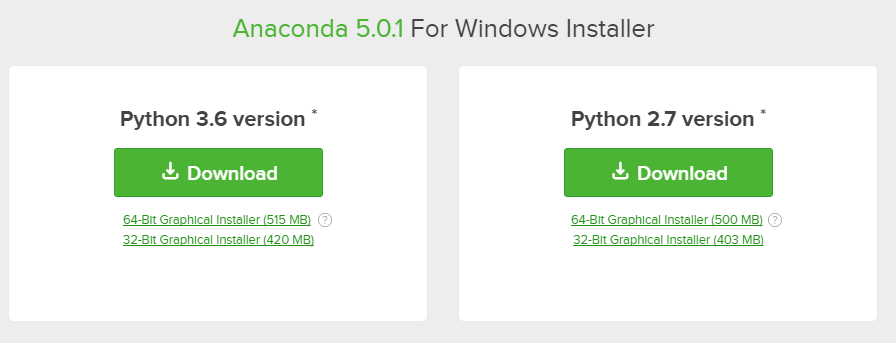
\includegraphics{images/anaconda_python3_or_python2.png}
\caption{Anaconda select Python 3.6}
\end{figure}

You may be prompted to enter your email. You can still download Anaconda
if you click \lstinline![No Thanks]! and don't enter your Work Email
address.

\begin{figure}
\centering
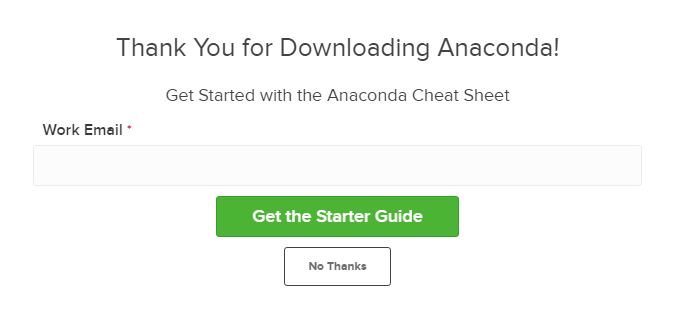
\includegraphics{images/anaconda_enter_email.png}
\caption{anaconda}
\end{figure}

The download is quite large (over 500 MB) so it may take a while to
complete

\begin{figure}
\centering

\includegraphics{images/anaconda_downloading.png}
\caption{anaconda downloading}
\end{figure}
    




    
        \subsubsection{4. Open and run the
installer}\label{open-and-run-the-installer}

Once the download completes, open and run the \textbf{\emph{.exe}}
installer

\begin{figure}
\centering
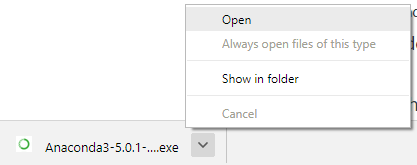
\includegraphics{images/anaconda_run_installer.png}
\caption{anaconda installer}
\end{figure}

At the beginning of the install, you need to click \textbf{Next} to
confirm the installation.

\begin{figure}
\centering
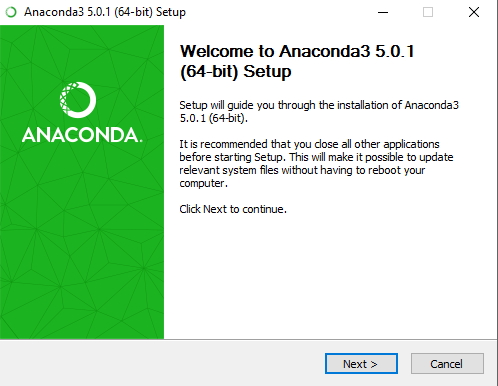
\includegraphics{images/anaconda_installer_click_next.png}
\caption{anaconda installer click next}
\end{figure}

Then agree to the license.

\begin{figure}
\centering
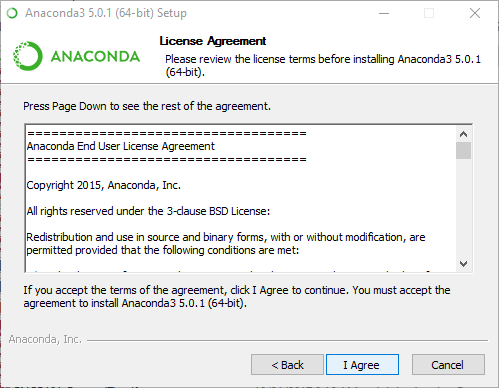
\includegraphics{images/anaconda_agree_to_license.png}
\caption{anaconda license}
\end{figure}

At the Advanced Installation Options screen, I recommend that you
\textbf{do not check} ``Add Anaconda to my PATH environment variable''

\begin{figure}
\centering
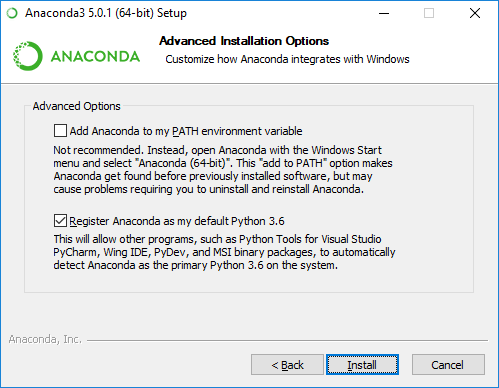
\includegraphics{images/anaconda_path2.png}
\caption{anaconda path variable}
\end{figure}
    




    
        \subsubsection{5. Open the Anaconda Prompt from the Windows start
menu}\label{open-the-anaconda-prompt-from-the-windows-start-menu}

After the installation of Anaconda is complete, you can go to the
Windows start menu and select the Anaconda Prompt.

\begin{figure}
\centering
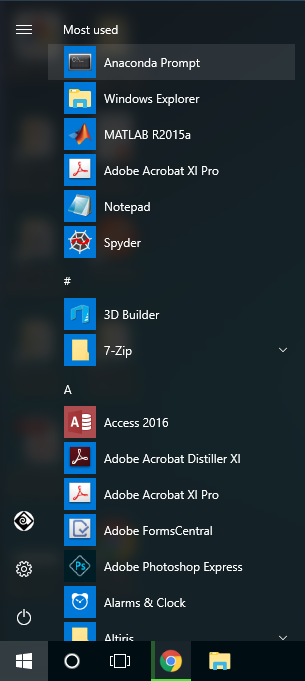
\includegraphics{images/anaconda_from_start_menu.png}
\caption{anaconda in start menu}
\end{figure}

This will open up the \textbf{Anaconda Prompt}, which is often called
the \textbf{conda prompt}. \textbf{Anaconda} is the Python distribution
and the \textbf{Anaconda Prompt} is a command line shell (a program
where you type in your commands instead of using a mouse). The black
screen and text that makes up the \textbf{Anaconda Prompt} doesn't look
like much, but it is really helpful for an undergraduate engineer using
Python.

At the Anaconda prompt, type \lstinline!python!. This will start the
Python interpreter, also called the Python REPL (for Read Evaluate Print
Loop).

\begin{lstlisting}
> python
\end{lstlisting}

\begin{figure}
\centering
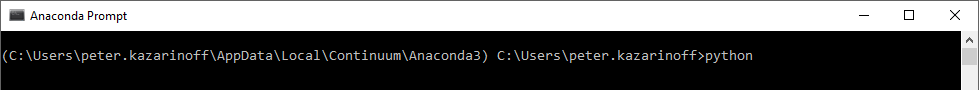
\includegraphics{images/conda_prompt_type_python.png}
\caption{conda prompt type python}
\end{figure}

Note the Python version. You should see something like
\lstinline!Python 3.6.1!. With the interpreter running, you will see a
set of greater-than symbols \lstinline!>>>! before the cursor.

\begin{figure}
\centering
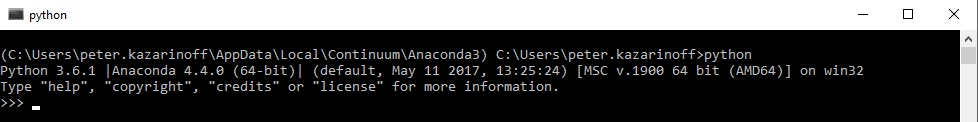
\includegraphics{images/conda_type_python.png}
\caption{anaconda prompt}
\end{figure}

Now you can type Python commands. Try typing \lstinline!import this!.
You should see the \textbf{\emph{Zen of Python}} by Tim Peters

\begin{figure}
\centering
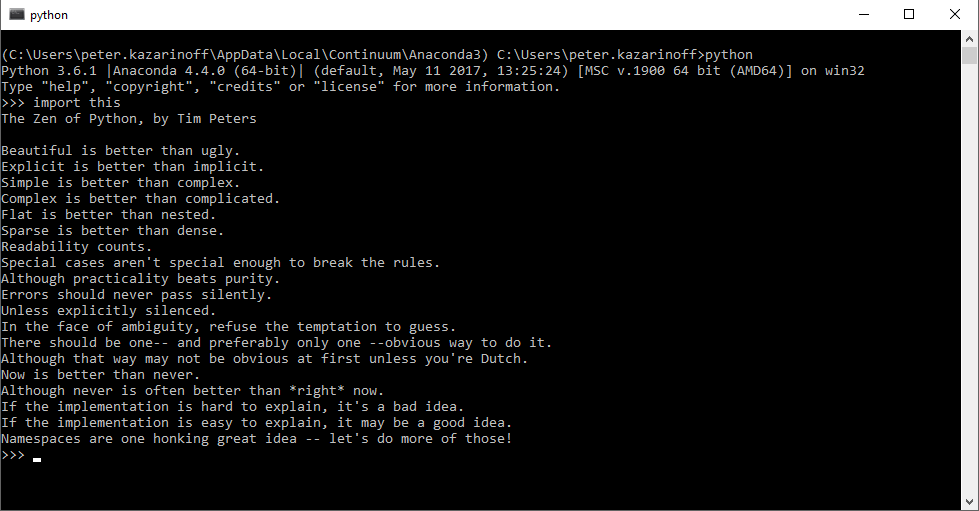
\includegraphics{images/conda_import_this_output.png}
\caption{anaconda\_import\_this}
\end{figure}

To close the Python interpreter, type \lstinline!exit()! at the prompt
\lstinline!>>>!. Note the double parenthesis at the end of the
\lstinline!exit()! command. The \lstinline!()! is needed to stop the
Python interpreter and get back out to the \textbf{Anaconda Prompt}.

To close the \textbf{Anaconda Prompt}, you can either close the window
with the mouse, or type \lstinline!exit!, no parenthesis necessary.

When you want to use the Python interpreter again, just click the
Windows Start button and select the \textbf{Anaconda Prompt} and type
\lstinline!python!.
    




    
        \section{Installing Anaconda on
MacOS}\label{installing-anaconda-on-macos}
    




    
        This section details the installation of the Anaconda Distribution of
Python on MacOS. Most versions of MacOS come pre-installed with legacy
Python (Version 2.7). You can confirm this legacy version of Python is
installed by opening and running a command at the MacOS
\textbf{terminal}. To open the MacOS terminal use
\lstinline![command]+[Space Bar]! and type \lstinline!terminal! in the
Spotlight Search bar.

In the MacOS Terminal type (note: the dollar sign \lstinline!$! is used
to indicate the terminal prompt. The dollar sign \lstinline!$! does not
need to be typed):

\begin{lstlisting}
$ python
\end{lstlisting}

You will most likely see version 2.7 is installed. An issue for MacOS
users is that the installed system version of Python has a set of
permissions that will not always allow Python to run and may not allow
Python to install external packages. Therefore, I recommend the Anaconda
Distribution of Python is installed alongside the system version of
Python that comes with MacOS. You will be able to run Python code using
the Anaconda Distribution of Python, and you will be able to install
external packages on the Anaconda Distribution of Python.

To install the Anaconda Distribution of Python, follow the steps below:

\subsubsection{Steps:}\label{steps}

\begin{enumerate}
\def\labelenumi{\arabic{enumi}.}
\item
  Visit
  \href{https://www.anaconda.com/download/}{Anaconda.com/downloads}
\item
  Select MacOS and Download the \textbf{\emph{.pkg}} installer
\item
  Open the \textbf{\emph{.pkg}} installer
\item
  Follow the installation instructions
\item
  Source your \textbf{\emph{.bash-rc}} file
\item
  Open a terminal and type \lstinline!python! and run some code.
\end{enumerate}
    




    
        \subsubsection{1. Visit the Anaconda downloads
page}\label{visit-the-anaconda-downloads-page}

Go to the following link:
\href{https://www.anaconda.com/download/}{Anaconda.com/downloads}

The Anaconda Downloads Page will look something like this:

\begin{figure}
\centering

\includegraphics{images/anaconda_download_page.png}
\caption{anaconda download page}
\end{figure}
    




    
        \subsubsection{2. Select MacOS and download the .pkg
installer}\label{select-macos-and-download-the-.pkg-installer}

In the operating systems box, select \lstinline![MacOS]!. Then download
the most recent Python 3 distribution (at the time of this writing the
most recent version is Python 3.6) graphical installer by clicking the
Download link. Python 2.7 is legacy Python. For problem solvers, select
the most recent Python 3 version.

\begin{figure}
\centering
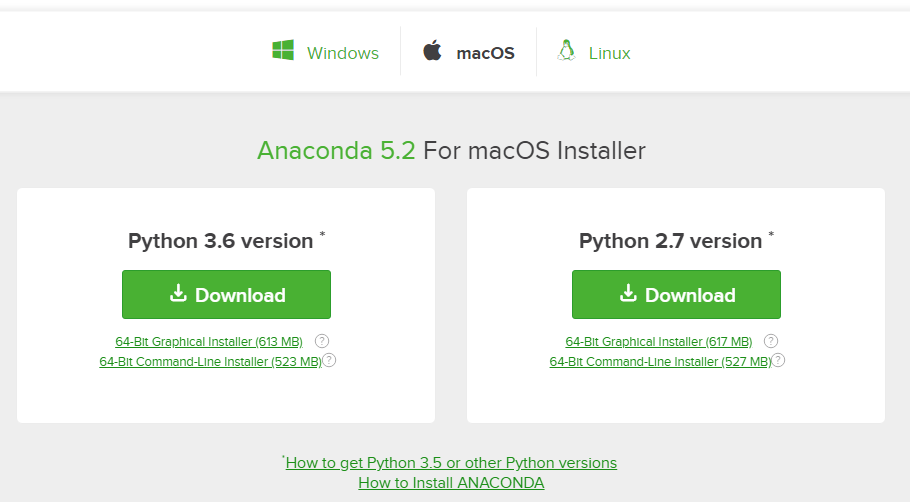
\includegraphics{images/anaconda_download_mac.png}
\caption{Anaconda Select Python 3.6}
\end{figure}

You may be prompted to enter your email. You can still download Anaconda
if you click \lstinline![No Thanks]! or \lstinline![x]! and don't enter
your Work Email address.

\begin{figure}
\centering
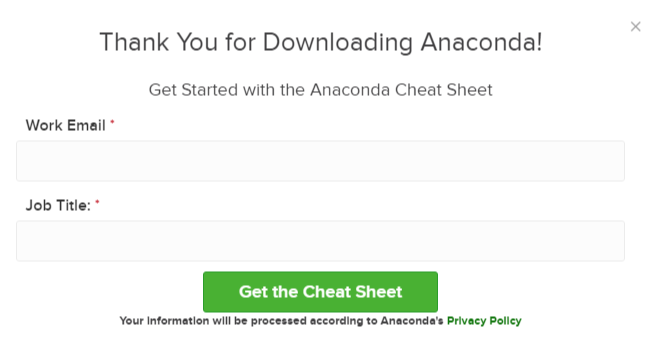
\includegraphics{images/anaconda_download_mac_ask_for_email.png}
\caption{Anaconda ask for email}
\end{figure}
    




    
        \subsubsection{3. Open the .pkg
installer}\label{open-the-.pkg-installer}

Using the MacOS Finder, navigate to the downloads folder and
double-click the \textbf{\emph{.pkg}} installer file you just
downloaded. It may be helpful to order your downloads by date to find
the \textbf{\emph{.pkg}} file.
    




    
        \subsubsection{4. Follow the installation
instructions}\label{follow-the-installation-instructions}

Follow the installation instructions. It is advised that you install
\textbf{Anaconda} for the current user and that \textbf{Anaconda}
\textbf{is added to your PATH}.
    




    
        \subsubsection{5. Source your .bash-rc
file}\label{source-your-.bash-rc-file}

Once Anaconda is installed, you need to load the changes to your
\lstinline!PATH! environment variable in the current terminal session.

Open the MacOS Terminal and type:

\begin{lstlisting}
$ cd ~
$ source .bashrc
\end{lstlisting}
    




    
        \subsubsection{\texorpdfstring{6. Open a terminal and type
\texttt{python} and run some
code.}{6. Open a terminal and type python and run some code.}}\label{open-a-terminal-and-type-python-and-run-some-code.}

Open the MacOS Terminal and type:

\begin{lstlisting}
$ python
\end{lstlisting}

You should see something like

\begin{lstlisting}
Python 3.6.3 | Anaconda Inc. |
\end{lstlisting}

At the Python REPL (the Python \lstinline!>>>! prompt) try:

\begin{lstlisting}
>>> import this
\end{lstlisting}

If you see the Zen of Python, the installation was successful. Exit out
of the Python REPL using \lstinline!>>> exit()!. Make sure to include
the double parenthesis \lstinline!()! after the \lstinline!exit!
command.
    




    
        \section{Installing Anaconda on
Linux}\label{installing-anaconda-on-linux}
    




    
        This section details the installation of the Anaconda distribution of
Python on Linux, specifically Ubuntu 16.04, but the instructions should
work for other Debian-based Linux distributions as well.

Ubuntu 16.04 comes pre-installed with Python (Version 3.3) and legacy
Python (Version 2.7). You can confirm the legacy version of Python is
installed by opening up a terminal.

In the terminal type:

\begin{lstlisting}
$ python
\end{lstlisting}

You will most likely see version 2.7 is installed. If you enter:

\begin{lstlisting}
$ python3
\end{lstlisting}

You will most likely see version 3.3 is installed. You can use this
version of Python, but each time a new package needs to be downloaded,
the \lstinline!$ pip3 install! command must be used.

Install the Anaconda distribution of Python to follow the examples in
the book without the need to install additional third-party packages.
    




    
        \subsubsection{Steps:}\label{steps}

\begin{enumerate}
\def\labelenumi{\arabic{enumi}.}
\item
  Visit
  \href{https://www.anaconda.com/download/}{Anaconda.com/downloads}
\item
  Select Linux
\item
  Copy the bash (.sh file) installer link
\item
  Use \lstinline!wget! to download the bash installer
\item
  Run the bash script to install \textbf{Anaconda3}
\item
  \lstinline!source! the \lstinline!.bash-rc! file to add Anaconda to
  your \lstinline!PATH!
\item
  Start the Python REPL
\end{enumerate}
    




    
        \subsection{1. Visit the Anaconda downloads
page}\label{visit-the-anaconda-downloads-page}

Go to the following link:
\href{https://www.anaconda.com/download/}{Anaconda.com/downloads}

The Anaconda Downloads Page will look something like this:

\begin{figure}
\centering

\includegraphics{images/anaconda_download_page.png}
\caption{Anaconda Downloads Page}
\end{figure}
    




    
        \subsection{2. Select Linux}\label{select-linux}

On the downloads page, select the Linux operating system

\begin{figure}
\centering

\includegraphics{images/Anaconda_download_linux.png}
\caption{anaconda\_install\_linux}
\end{figure}
    




    
        \subsection{3. Copy the bash (.sh file) installer
link}\label{copy-the-bash-.sh-file-installer-link}

In the \textbf{Python 3.6 Version* } box, right-click on the
{[}64-Bit(x86) Installer{]} link. Select {[}copy link address{]}.

\begin{figure}
\centering
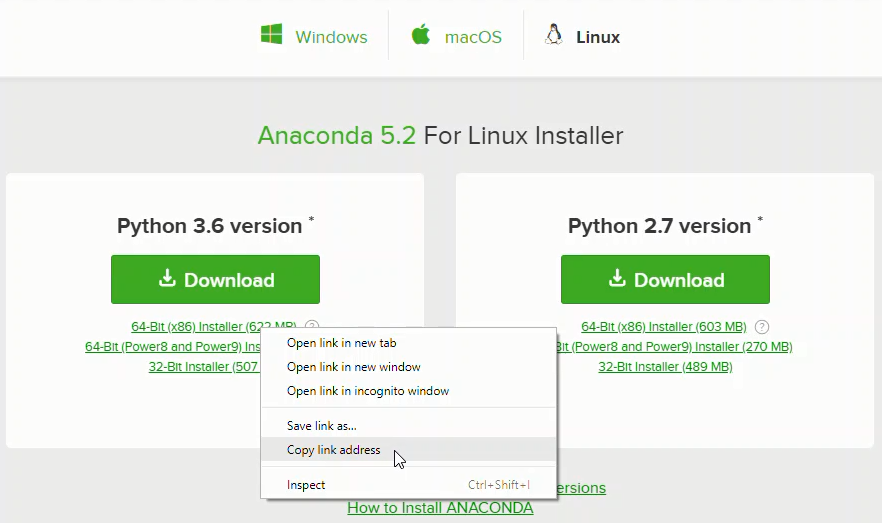
\includegraphics{images/anaconda_install_linux_copy_link_address.png}
\caption{Anaconda installation on Linux copy link address}
\end{figure}
    




    
        \subsection{\texorpdfstring{4. Use \texttt{wget} to download the bash
installer}{4. Use wget to download the bash installer}}\label{use-wget-to-download-the-bash-installer}

Now that the bash installer (.sh file) link is stored on the clipboard,
use \lstinline!wget! to download the installer script. In a terminal,
\lstinline!cd! into the home directory and make a new directory called
\lstinline!tmp!. \lstinline!cd! into \lstinline!tmp! and use
\lstinline!wget! to download the installer. Although the installer is a
bash script, it is still quite large and the download will not be
immediate.

\begin{lstlisting}
$ cd ~
$ mkdir tmp
$ cd tmp
$ wget https://repo.anaconda.com/archive/Anaconda3-5.2.0-Linux-x86_64.sh 
\end{lstlisting}
    




    
        \subsection{\texorpdfstring{5. Run the bash script to install
\textbf{Anaconda3}}{5. Run the bash script to install Anaconda3}}\label{run-the-bash-script-to-install-anaconda3}

With the bash installer script downloaded, run the \textbf{\emph{.sh}}
script to install \textbf{Anaconda3}. Ensure you are in the directory
where the installer script downloaded:

\begin{lstlisting}
$ ls
Anaconda3-5.2.0-Linux-x86_64.sh
\end{lstlisting}

Run the installer script with bash

\begin{lstlisting}
$ bash Anaconda3-5.2.0-Linux-x86_64.sh
\end{lstlisting}

Accept the Licence Agreement and allow Anaconda to be added to your
\lstinline!PATH!. By adding Anaconda to your \lstinline!PATH! the
Anaconda distribution of Python will be called when you type
\lstinline!$ python!.
    




    
        \subsubsection{\texorpdfstring{6. \texttt{source} the \texttt{.bash-rc}
file to add Anaconda to your
\texttt{PATH}}{6. source the .bash-rc file to add Anaconda to your PATH}}\label{source-the-.bash-rc-file-to-add-anaconda-to-your-path}

Now that \textbf{Anaconda3} is installed and \textbf{Anaconda3} is added
to our \lstinline!PATH!, \lstinline!source! the \lstinline!.bashrc! file
to load the new \lstinline!PATH! environment variable into the current
terminal session. Note the \lstinline!.bashrc! file is in the home
directory. You can see it with \lstinline!$ ls -a!.

\begin{lstlisting}
$ cd ~
$ source .bashrc
\end{lstlisting}
    




    
        \subsubsection{7. Start the Python REPL}\label{start-the-python-repl}

To verify the installation is complete, open Python from the command
line:

\begin{lstlisting}
$ python

Python 3.6.5 |Anaconda, Inc.| (default, Mar 29 2018, 18:21:58)
[GCC 7.2.0] on linux
Type "help", "copyright", "credits" or "license" for more information.
>>>
\end{lstlisting}

If you see Python 3.6 from Anaconda listed, your installation is
complete. To exit the Python REPL, type:

\begin{lstlisting}
>>> exit()
\end{lstlisting}
    




    
        \section{Installing Python from
Python.org}\label{installing-python-from-python.org}
    




    
        Below are the recommended ways to install a new version of Python from
Python.org on the three major operating systems: Windows, MacOS and
Linux. This book is based on Python version 3.6. Some of the problems
may not work properly on legacy Python (version 2.7). I recommend using
the Anaconda Distribution of Python on Windows and MacOSX. The
installation of Anaconda on these operating systems was detailed in
previous sections.
    




    
        \subsection{Installing Python on
Windows}\label{installing-python-on-windows}

Go to \url{https://www.python.org/downloads/} and download the latest
release. Make sure to select the box {[}add Python to my path{]}.

\begin{figure}
\centering
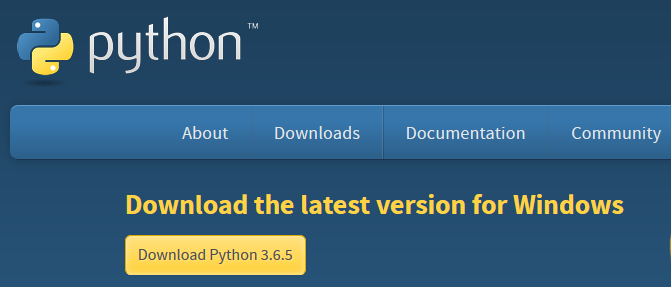
\includegraphics{images/python_dot_org_windows_download.PNG}
\caption{Python.org download for Windows}
\end{figure}
    




    
        \subsection{Installing Python on Mac
OSX}\label{installing-python-on-mac-osx}

Go to \url{https://www.python.org/downloads/mac-osx/} and download the
latest release.

\begin{figure}
\centering

\includegraphics{images/python_dot_org_macos_download.PNG}
\caption{Python.org download for MacOS}
\end{figure}
    




    
        \subsection{Installing Python on
Linux}\label{installing-python-on-linux}

Open a terminal and enter \lstinline!$ python! to see if a version of
Python is already installed on the system.

\begin{lstlisting}
$ python
Python 2.7.12 (default, Dec  4 2017, 14:50:18)
[GCC 5.4.0 20160609] on linux2
Type "help", "copyright", "credits" or "license" for more information.
>>> exit()
\end{lstlisting}

In the code block above the version of Python is
\lstinline!Python 2.7.12!. If the Python version is 2.7 or below, try
the command \lstinline!$ python3!.

\begin{lstlisting}
$ python3
Python 3.5.2 (default, Nov 23 2017, 16:37:01) 
[GCC 5.4.0 20160609] on linux
Type "help", "copyright", "credits" or "license" for more information.
>>> exit()
\end{lstlisting}

If no version of Python is shown, you can download a release of Python
3.6 from the deadsnakes package repository.

\begin{lstlisting}
$ sudo add-apt-repository ppa:deadsnakes/ppa
$ [Enter]
$ sudo apt-get update
$ sudo apt-get install python3.6
\end{lstlisting}

After installation, you may need to append your PATH environment
variable to ensure the newly installed Python 3.6 version is the version
of Python called when using the terminal. The commands below will add
\lstinline!/usr/bin! to \lstinline!PATH!, and add an alias in
\textbf{\emph{.bashrc}} so that the command \lstinline!$ python3.6!
produces the Python 3.6 REPL. Take care to ensure the double chevron
\lstinline!>>! is used, as a single chevron \lstinline!>! will overwrite
the \textbf{\emph{.bashrc}} file.

\begin{lstlisting}
$ cd ~
$ echo  'PATH=/usr/bin:$PATH' >> ~/.bashrc 
$ echo "alias python3.6='/usr/bin/python3.6'" >> ~/.bashrc
$ source .bashrc
$ python3.6
Python 3.6.6 (default, Jun 28 2018, 04:42:43)
[GCC 5.4.0 20160609] on linux
Type "help", "copyright", "credits" or "license" for more information.
>>> exit()
\end{lstlisting}
    




    
        \newpage
        \section{Summary}\label{summary}

    




    
        In this chapter, you learned how to install the \textbf{Anaconda}
distribution of Python on your computer.
    




    
        \subsection{Key Terms and Concepts}\label{key-terms-and-concepts}
    




    
        \begin{key_terms}
        Anaconda

Download

Install

Python

Operating System

Windows

MacOS

Linux

Terminal

PATH
        \end{key_terms}

    




    
        \section{Review Questions}\label{review-questions}
    




    
        \begin{problems}
        Q1.01 What is Python? How is the Python language different than the
Python Interpreter?

Q1.02 What is the difference between the version of Python at Python.org
and the version of Python at Anaconda.com?

Q1.03 Why does the text advise that undergraduate engineers use

Q1.04

Q1.05

Q1.06

Q1.07
        \end{problems}

    




    
        \chapter{The Python REPL}\label{the-python-repl}
    




    
        \section{Introduction}\label{introduction}
    




    
        By the end of this chapter, you will be able to:

\begin{itemize}
\item
  Open and close the Python REPL
\item
  Compute mathematical calculations using the Python REPL
\item
  Use the output from Python REPL as input in another problem
\item
  Import the math and statistics modules from the standard library and
  use their functions
\item
  Combine \lstinline!True! and \lstinline!False! in logical statements
\end{itemize}
        \newpage



    




    
        \section{Python as a Calculator}\label{python-as-a-calculator}
    




    
        Python can be used as a calculator to compute arithmetic operations like
addition, subtraction, multiplication and division. Python can also be
used for trigonometric calculations and statistical calculations.
    




    
        \subsection{Arithmetic}\label{arithmetic}

Python can be used as a calculator to make simple or complex
calculations.

We can do this easily with Python at the Python Prompt, also called the
\lstinline!Python REPL!. REPL stands for Read Evaluate Print Loop. The
Python REPL shows three arrow symbols \lstinline!>>>! after which you
will see a blinking cursor. Programmers type commands at the prompt then
hit {[}ENTER{]} to see the results. The commands are \emph{read} by the
interpreter, results of running the commands are \emph{evaluated}, then
\emph{printed} to the command window. After the output is printed, a new
\lstinline!>>>! prompt appears on a new line. This process repeats over
and over again in a continuous \emph{loop}.

Try the following commands at the Python REPL:

Suppose the mass of a battery is 5 kg and the mass of the battery cables
is 3 kg. What is the mass of the battery cable assembly?

\begin{lstlisting}[language=Python]
>>> 5 + 3
8
\end{lstlisting}

Suppose one of the cables above is removed and it has a mass of 1.5 kg.
What is the mass of the leftover assembly

\begin{lstlisting}[language=Python]
>>> 8 - 1.5
6.5
\end{lstlisting}

If the battery has a mass of 5000 g and a volume of 2500 \(cm^3\) What
is the density of the battery? The formula for density is below, where D
is density, m is mass and v is volume.

\[ D = \frac{m}{v} \]

In the problem above \(m = 5000\) and \(v=2500\)

Let's solve this with Python.

\begin{lstlisting}[language=Python]
>>> 5000 / 2500
2.0
\end{lstlisting}

What is the total mass if we have 2 batteries, that each weight 5 kg?

\begin{lstlisting}[language=Python]
>>> 5 * 2
2.0
\end{lstlisting}

The length, width, and height of each battery is 3 cm. What is the area
of the base of the battery? To complete this problem, use the double
asterisk symbol \lstinline!**! to raise a number to a power.

\begin{lstlisting}[language=Python]
>>> 3 ** 2
9
\end{lstlisting}

What is the volume of the battery if each the length, width, and height
of the battery are all 3 cm?

\begin{lstlisting}[language=Python]
>>> 3 ** 3
27
\end{lstlisting}

Find the mass of the two batteries and two cables.

We can use Python to find the mass of the batteries and then use the
answer, which Python saves as an underscore \_ to use in our next
operation. (The underscore \lstinline!_! in Python is comparable to the
\lstinline!ans! variable in MATLAB)

\begin{lstlisting}[language=Python]
>>> 2 * 5 
10
>>> _ + 1.5 + 1
12.5
\end{lstlisting}
    




    
        \subsubsection{Section Summary}\label{section-summary}

A summary of the arithmetic operations in Python is below:

\begin{longtable}[]{@{}lllll@{}}
\toprule
operator & name & description & example & result\tabularnewline
\midrule
\endhead
\lstinline!+! & addition & adds two numbers & \lstinline!2 + 3! &
\lstinline!5!\tabularnewline
\lstinline!-! & subtraction & subtracts two numbers & \lstinline!8 - 6!
& \lstinline!2!\tabularnewline
\lstinline!-! & negation & negative number & \lstinline!-4! &
\lstinline!-4!\tabularnewline
\lstinline!*! & multiplication & multiplies two numbers &
\lstinline!5 * 2! & \lstinline!10!\tabularnewline
\lstinline!/! & division & divides two numbers & \lstinline!6 / 3! &
\lstinline!2!\tabularnewline
\lstinline!**! & exponents & raises a number to a power &
\lstinline!10**2! & \lstinline!100!\tabularnewline
\lstinline!_! & underscore & returns last saved value &
\lstinline!_ + 7! & \lstinline!107!\tabularnewline
\bottomrule
\end{longtable}
    




    
        \subsection{Trigonometry: sine, cosine, and
tangent}\label{trigonometry-sine-cosine-and-tangent}
    




    
        Trig functions such as sine, cosine, and tangent can also be calculated
using the Python REPL.

To use these functions, we need to introduce a new concept:
\emph{importing modules}.

In Python, there are many operations built into the language when it
starts. These include \lstinline!+! , \lstinline!-!, \lstinline!*!,
\lstinline!/! like we saw in the previous section. However, not all
functions will work right away when Python starts. Say we want to find
the sine of an angle. Try the following:

\begin{lstlisting}[language=Python]
>>> sin(60)
Traceback (most recent call last):
  File "<stdin>", line 1, in <module>
NameError: name 'sin' is not defined
\end{lstlisting}

This error results because we have not told Python to include the
\lstinline!sin! function. The \lstinline!sin! function is part of the
\emph{Python Standard Library}. The Python Standard Library comes with
every python installation and includes many functions, but not all of
these functions are available to us when we start a new Python REPL
session. To use the \lstinline!sin! function, first import the
\lstinline!sin! function from the \lstinline!math! \emph{module} which
is part of the Python Standard Library.

Importing modules and functions is easy. Use the following syntax: from
\emph{module name} import \emph{function name}

To import the \lstinline!sin()! function from the \lstinline!math!
module try:

\begin{lstlisting}[language=Python]
>>> from math import sin
>>> sin(60)
-0.3048106211022167
\end{lstlisting}

Success! Multiple modules can be imported at the same time. Say we want
to use a bunch of different trig functions to solve the following
problem.

An angle has a value of \(\pi\)/6 radians. What is the sine, cos, and
tangent of the angle?

To solve this problem we need to import the \lstinline!sin()!,
\lstinline!cos()!, and \lstinline!tan()! functions. It is also useful to
have the value of \(\pi\), rather than having to write
\lstinline!3.14....! We can import all of these functions at the same
time using the syntax
\lstinline!from <module> import <function1>, <function2>, <function3>!.
Note the commas in between the function names.

Try:

\begin{lstlisting}[language=Python]
>>> from math import sin, cos, tan, pi
>>> pi
3.141592653589793
>>> pi/4
0.7853981633974483
>>> sin(pi/4)
0.7853981633974483
>>> sin(2*pi)
\end{lstlisting}
    




    
        \subsubsection{Section Summary}\label{section-summary}

The following trig functions are part of Python's \textbf{math} module:

\begin{longtable}[]{@{}lllll@{}}
\toprule
trig function & name & description & example & result\tabularnewline
\midrule
\endhead
\lstinline!math.pi! & pi & mathematical constant \(\pi\) &
\lstinline!math.pi! & \lstinline!3.14!\tabularnewline
\lstinline!math.sin()! & sine & sine of an angle in radians &
\lstinline!math.sin(4)! & \lstinline!9.025!\tabularnewline
\lstinline!math.cos()! & cosine & cosine of an angle in radians &
\lstinline!cos(3.1)! & \lstinline!400!\tabularnewline
\lstinline!math.tan()! & tangent & tangent of an angle in radians &
\lstinline!tan(100)! & \lstinline!2.0!\tabularnewline
\lstinline!math.asin()! & arc sine & inverse sine, ouput in radians &
\lstinline!math.sin(4)! & \lstinline!9.025!\tabularnewline
\lstinline!math.acos()! & arc cosine & inverse cosine, ouput in radians
& \lstinline!log(3.1)! & \lstinline!400!\tabularnewline
\lstinline!math.atan()! & arc tangent & inverse tangent, ouput in
radians & \lstinline!atan(100)! & \lstinline!2.0!\tabularnewline
\lstinline!math.radians()! & radians conversion & degrees to radians &
\lstinline!math.radians(90)! & \lstinline!1.57!\tabularnewline
\lstinline!math.degress()! & degree conversion & radians to degrees &
\lstinline!math.degrees(2)! & \lstinline!114.59!\tabularnewline
\bottomrule
\end{longtable}
    




    
        \subsection{Exponents and Logarithms}\label{exponents-and-logarithms}

Calculating exponents and logarithms with Python is easy. Note the
exponent and logarithm functions are imported from the \textbf{math}
module just like the trig functions were imported from the \textbf{math}
module above.

The following functions can be imported from the math module:

\begin{itemize}
\tightlist
\item
  \lstinline!log!
\item
  \lstinline!log10!
\item
  \lstinline!exp!
\item
  \lstinline!e!
\item
  \lstinline!pow(x,y)!
\item
  \lstinline!sqrt!
\end{itemize}

Let's try a couple of examples:

\begin{lstlisting}[language=Python]
>>> from math import log, log10, exp, e, pow, sqrt
>>> log(3.0*e**3.4)         # note: natural log
4.4986122886681095
\end{lstlisting}

A right triangle has side lengths 3 and 4. What is the length of the
hypotenuse?

\begin{lstlisting}[language=Python]
>>> sqrt(3**2 + 4**2)
5.0 
\end{lstlisting}

The power function \lstinline!pow()! works like the \lstinline!**!
operator to raise a number to a power.

\begin{lstlisting}[language=Python]
>>> 5**2
25
\end{lstlisting}

\begin{lstlisting}[language=Python]
>>> pow(5,2)
25.0
\end{lstlisting}

\subsubsection{Section Summary}\label{section-summary}

The following exponent and logarithm functions are part of the
\textbf{math} module:

\begin{longtable}[]{@{}lllll@{}}
\toprule
math module function & name & description & example &
result\tabularnewline
\midrule
\endhead
\lstinline!math.e! & euler's number & mathematical constant \(e\) &
\lstinline!math.e! & \lstinline!2.718!\tabularnewline
& & & &\tabularnewline
\lstinline!math.exp()! & exponent & \(e\) raised to a power &
\lstinline!math.exp(2.2)! & \lstinline!9.025!\tabularnewline
\lstinline!math.log()! & natural logerithm & log base e &
\lstinline!math.log(3.1)! & \lstinline!400!\tabularnewline
\lstinline!math.log10()! & base 10 logerithm & log base 10 &
\lstinline!math.log10(100)! & \lstinline!2.0!\tabularnewline
\lstinline!math.pow()! & exponents & raises a number to a power &
\lstinline!math.pow(2,3)! & \lstinline!8.0!\tabularnewline
\lstinline!math.sqrt()! & square root & square root of a number &
\lstinline!math.sqrt(16)! & \lstinline!4.0!\tabularnewline
\bottomrule
\end{longtable}
    




    
        \subsection{Statistics}\label{statistics}

To round out this section, we will look at a couple of statistics
functions. These functions are part of the Python Standard Library, but
not part of the \textbf{math} module. To access Python's statistics
functions, we need to import them from the \textbf{statistics} module
using the statement
\lstinline!from statistics import mean, median, mode, stdev!. Then the
functions \lstinline!mean!, \lstinline!median!, \lstinline!mode! and
\lstinline!stdev!(standard deviation) can be used.

\begin{lstlisting}[language=Python]
>>> from statistics import mean, median, mode, stdev
    
>>> test_scores = [ 60 , 83, 83, 91, 100]
    
>>> mean(test_scores)
83.4

>>> median(test_scores)
83

>>> mode(test_scores)
83
    
>>> stdev(test_scores)
14.842506526863986 
\end{lstlisting}

Alternatively, we can import the entire \textbf{statistics} module using
the statement \lstinline!import statistics!. Then to use the functions,
we need to use the names \lstinline!statistics.mean!,
\lstinline!statistics.median!, \lstinline!statistics.mode!, and
\lstinline!statistics.stdev!. See below:

\begin{lstlisting}[language=Python]
>>> import statistics
    
>>> test_scores = [ 60 , 83, 83, 91, 100]
    
>>> statistics.mean(test_scores)
83.4

>>> statistics.median(test_scores)
83

>>> statistics.mode(test_scores)
83
    
>>> statistics.stdev(test_scores)
14.842506526863986 
\end{lstlisting}
    




    
        \subsubsection{Section Summary}\label{section-summary}

The following functions are part of the \textbf{statistics} module:

\begin{longtable}[]{@{}lllll@{}}
\toprule
statistics module function & name & description & example &
result\tabularnewline
\midrule
\endhead
\lstinline!mean()! & mean & mean or average &
\lstinline!mean([1,4,5,5])! & \lstinline!3.75!\tabularnewline
\lstinline!median()! & median & middle value &
\lstinline!median([1,4,5,5])! & \lstinline!4.5!\tabularnewline
\lstinline!mode()! & mode & most often & \lstinline!mode([1,4,5,5])! &
\lstinline!5!\tabularnewline
\lstinline!stdev()! & standard deviation & spread of data &
\lstinline!stdev([1,4,5,5])! & \lstinline!1.892!\tabularnewline
\lstinline!variance()! & variance & variance of data &
\lstinline!variance([1,4,5,5])! & \lstinline!3.583!\tabularnewline
\bottomrule
\end{longtable}
    




    
        \section{Variables}\label{variables}
    




    
        Variables are assigned in Python using the \lstinline!=! equals sign
also called the assignment operator. The statement:

\begin{lstlisting}[language=Python]
a = 2
\end{lstlisting}

Assigns the integer \lstinline!2! to the variable \lstinline!a!.
    




    
        \begin{lstlisting}[language=Python]
>>> a = 2
>>> a
2
\end{lstlisting}
    




    
        Note the assignment operator \lstinline!=!(equals), is different from
the logical comparison operator \lstinline!==! (equivalent to).
    




    
        \begin{lstlisting}[language=Python]
>>> a == 2
True
\end{lstlisting}
    




    
        Variable names in Python must follow the rules below:

\begin{itemize}
\tightlist
\item
  variable names must start with a letter
\item
  variable names only contain letters, numbers, and the underscore
  character \lstinline!_!
\item
  variable names can not contain spaces
\item
  variable names are not enclosed in quotes or brackets
\end{itemize}
    




    
        The following are valid variable names:
    



    \begin{Verbatim}[commandchars=\\\{\}]
{\color{incolor}In [{\color{incolor}2}]:} \PY{n}{constant} \PY{o}{=} \PY{l+m+mi}{4}
        
        \PY{n}{new\PYZus{}variable} \PY{o}{=} \PY{l+s+s1}{\PYZsq{}}\PY{l+s+s1}{var}\PY{l+s+s1}{\PYZsq{}}
        
        \PY{n}{my2rules} \PY{o}{=} \PY{p}{[}\PY{l+s+s1}{\PYZsq{}}\PY{l+s+s1}{rule1}\PY{l+s+s1}{\PYZsq{}}\PY{p}{,}\PY{l+s+s1}{\PYZsq{}}\PY{l+s+s1}{rule2}\PY{l+s+s1}{\PYZsq{}}\PY{p}{]}
        
        \PY{n}{SQUARES} \PY{o}{=} \PY{l+m+mi}{4}
\end{Verbatim}



    
        The following are invalid variable names:
    



    \begin{Verbatim}[commandchars=\\\{\}]
{\color{incolor}In [{\color{incolor}3}]:} \PY{n}{a} \PY{n}{constant} \PY{o}{=} \PY{l+m+mi}{4}
        
        \PY{l+m+mi}{3}\PY{n}{newVariables} \PY{o}{=} \PY{p}{[}\PY{l+m+mi}{1}\PY{p}{,} \PY{l+m+mi}{2}\PY{p}{,} \PY{l+m+mi}{3}\PY{p}{]}
        
        \PY{o}{\PYZam{}}\PY{n+nb}{sum} \PY{o}{=} \PY{l+m+mi}{4} \PY{o}{+} \PY{l+m+mi}{4}
        
        \PY{c+c1}{\PYZsh{}a\PYZus{}new\PYZus{}variable = 6}
\end{Verbatim}


    \begin{Verbatim}[commandchars=\\\{\}]

          File "<ipython-input-3-d6921874e142>", line 1
        a constant = 4
                 \^{}
    SyntaxError: invalid syntax
    

    \end{Verbatim}


    
        Problem: The Arrhenius relationship states that

\[ n = n_{v}e^{-Q_v/(RT)} \]

We can use variables to assign a value to each one of the constants in
the problem.

\begin{lstlisting}[language=Python]
>>> nv = 2.0**(-0.3)
>>> Qv = 5
>>> R = 3.18
>>> T = 293
>>> n = nv*e**(-1*Qv/(R*T))
>>> n
0.8079052775625613
\end{lstlisting}
    




    
        \section{Boolean Arithmetic}\label{boolean-arithmetic}
    




    
        \emph{Boolean Arithmetic} is the arithmetic of true and false logic. A
\emph{boolean} or logical value can either be \lstinline!True! or
\lstinline!False!. In Python, the keywords \lstinline!True! and
\lstinline!False! denote a boolean variable. Note that assigning
\lstinline!true! or \lstinline!false! to a variable will produce an
error.
    




    
        \begin{lstlisting}[language=Python]
>>> A = True
>>> B = False
\end{lstlisting}

\begin{lstlisting}[language=Python]
>>> A
True
\end{lstlisting}

\begin{lstlisting}[language=Python]
>>> B
False
\end{lstlisting}

\begin{lstlisting}[language=Python]
>>> A or B
True
\end{lstlisting}

\begin{lstlisting}[language=Python]
>>> A and B
False
\end{lstlisting}

\begin{lstlisting}[language=Python]
>>> not A
False
\end{lstlisting}

\begin{lstlisting}[language=Python]
>>> not B
True
\end{lstlisting}

\begin{lstlisting}[language=Python]
>>> A == B
False
\end{lstlisting}

\begin{lstlisting}[language=Python]
>>> A != B
True
\end{lstlisting}

\begin{lstlisting}[language=Python]
>>> C = False
>>> A or (C and B)
True
>>> (A and B) or C
False
\end{lstlisting}
    




    
        \section{String Operations}\label{string-operations}
    




    
        Some operations we can do on strings include indexing, concatenation,
and logical comparisons.
    




    
        \subsection{Indexing}\label{indexing}
    




    
        \begin{lstlisting}[language=Python]
>>> word = 'Solution'
>>> word[0]
'S'
\end{lstlisting}
    




    
        \begin{lstlisting}[language=Python]
>>> word[2]
'1'
\end{lstlisting}
    




    
        \begin{lstlisting}[language=Python]
>>> word[-1]
'n'
\end{lstlisting}
    




    
        \begin{lstlisting}[language=Python]
>>> word[0:3]
'Sol'
\end{lstlisting}
    




    
        \begin{lstlisting}[language=Python]
>>> word[:]
'Solution'
\end{lstlisting}
    




    
        \begin{lstlisting}[language=Python]
>>> word[-3:-1]  #not including ending
'io'
\end{lstlisting}
    




    
        \begin{lstlisting}[language=Python]
>>> word[0:8:2]  #start:stop+1:step
'Slto'
\end{lstlisting}
    




    
        \begin{lstlisting}[language=Python]
>>> word[::-1] # start=not specified :stop=not specified:step=-1
'noituloS'
\end{lstlisting}
    




    
        \section{Print Statements}\label{print-statements}
    




    
        The \lstinline!print()! function useful in Python. Below is a code
example:

\begin{lstlisting}[language=Python]
>>> name = Kendra
>>> print('Your name is: ')
Your name is
>>> print(name)
Kendra
\end{lstlisting}
    




    
        \newpage
        \section{Summary}\label{summary}

    




    
        In this chapter, you learned how to use the Python REPL, also called the
Python prompt, to solve calculation problems. You learned how to do
arithmetic, powers and logarithms, trigonometry and save values to
variables.
    




    
        \subsection{Key Terms and Concepts}\label{key-terms-and-concepts}

\begin{longtable}[]{@{}l@{}}
\toprule
Key Terms and Concepts\tabularnewline
\midrule
\endhead
REPL\tabularnewline
Operator\tabularnewline
Mathematical Operator\tabularnewline
Command Line\tabularnewline
Error\tabularnewline
Module\tabularnewline
Standard Library\tabularnewline
Import\tabularnewline
\bottomrule
\end{longtable}
    




    
        \subsection{Summary of Python Functions and
Commands}\label{summary-of-python-functions-and-commands}

Below is a summary of the functions and operators used in this chapter:

\subsubsection{Arithmetic}\label{arithmetic}

\begin{longtable}[]{@{}ll@{}}
\toprule
Arithmetic Operators & description\tabularnewline
\midrule
\endhead
\lstinline!+! & Addition\tabularnewline
\lstinline!-! & Subtraction\tabularnewline
\lstinline!*! & Multiplication\tabularnewline
\lstinline!/! & Division\tabularnewline
\lstinline!**! & Exponents\tabularnewline
\lstinline!_! & answer in memory\tabularnewline
\bottomrule
\end{longtable}

\subsubsection{Trigonometry}\label{trigonometry}

\begin{longtable}[]{@{}ll@{}}
\toprule
Trig Function & Description\tabularnewline
\midrule
\endhead
\lstinline!from math import *! &\tabularnewline
\lstinline!sin! & sine of angle in radians\tabularnewline
\lstinline!cos! & cosine of angle in radians\tabularnewline
\lstinline!tan! & tangent of angle in radians\tabularnewline
\lstinline!pi! & \(\pi\)\tabularnewline
\lstinline!degrees! & convert radians to degrees\tabularnewline
\lstinline!radians! & convert degrees to radians\tabularnewline
\lstinline!asin! & inverse sine\tabularnewline
\lstinline!acos! & inverse cosine\tabularnewline
\lstinline!atan! & inverse tangent\tabularnewline
\bottomrule
\end{longtable}

\subsubsection{Logarithms and Exponents}\label{logarithms-and-exponents}

\begin{longtable}[]{@{}ll@{}}
\toprule
Logarithms and Exponent Function & Description\tabularnewline
\midrule
\endhead
\lstinline!from math import *! &\tabularnewline
\lstinline!log! & log base e, natural log\tabularnewline
\lstinline!log10! & log base 10\tabularnewline
\lstinline!exp! & \(e^{power}\)\tabularnewline
\lstinline!e! & the math constant \(e\)\tabularnewline
\lstinline!pow(x,y)! & x raised to the y power\tabularnewline
\lstinline!sqrt! & square root\tabularnewline
\bottomrule
\end{longtable}

\subsubsection{Statistics}\label{statistics}

\begin{longtable}[]{@{}ll@{}}
\toprule
Statistical Function & Description\tabularnewline
\midrule
\endhead
\lstinline!from statistics import *! &\tabularnewline
\lstinline!mean! & mean (average)\tabularnewline
\lstinline!median! & median (middle value)\tabularnewline
\lstinline!mode! & (most often)\tabularnewline
\lstinline!stdev! & standard deviation of a sample\tabularnewline
\lstinline!pstdev! & standard deviation of a population\tabularnewline
\bottomrule
\end{longtable}
    




    
        \section{Review Questions}\label{review-questions}
    




    
        \begin{problems}
        Arithmetic

Q2.01 \(2 + \frac{1}{2}\)

Q2.02 \(4 \times 2 + \frac{2}{4}\)

Q2.03 \(\frac{5}{2} \times 3 + 4\)

Q2.04 \(4^2 + 3\)

Q2.05 \(\sqrt{16}\)

Q2.06 \(3^{4-5}\)

Q2.07 \(\frac{1+3+5}{2+4+6}\)

Q2.08 \(1 - 2 + \frac{9}{6} -3 + 5\)

Q2.09 \((3 + 5 -2)^{2/3}\)

Q2.10 \(\frac{5+3}{2 \times 5}\)

Q2.11 \(\sqrt{6^2 + 4}\)

Q2.12 \(1 + 9 \times \frac{8}{4^2} + 1^{3-4} \times \frac{1}{2.5}\)

Variables in Calculations

Q2.20 \(a = 2\), \(b = 3\), calculate \(\frac{4}{5}(a^2 - b^3)\)

Q2.21 The area of a circle, \(a\), is dependent on the circle's radius,
\(r\), according to \(a=\pi r^2\). What is the area of a circle with
radius \(r=4\)?

Q2.21 The area of a circle, \(a\), is dependent on the circle's
diameter, \(d\), according to \(a=\pi (\frac{d}{2})^2\). What is the
area of a circle with diameter \(d=6\)?

Q2.22 The volume of a sphere, \(v\), is dependent on the sphere's
radius, \(r\), according to \(v=(\frac{4}{2})\pi r^3\). What is the
volume of a sphere with radius \(r=1.5\)?

Q2.23 The volume of a cylinder, \(v\), is dependent on the cylinder's
radius, \(r\), and height, \(h\), according to \(v=\pi r^2 h\). What is
the volume of a cylinder with radius \(r=5\) and height \(h=10\)?

Q2.24 The surface area of a sphere, \(a_s\) is related to the sphere's
radius, \(r\), according to \(a_s=4\pi r^2\). What is the surface area
\(a_s\) of a sphere with radius \(r=2.5\)?

Q2.25 The general equation for the distance, \(d\), that a free falling
body travels (neglecting air resistance) is \(d = \frac{1}{2}gt^2\),
where \(g\) is the acceleration due to gravity and \(t\) is the fall
time. Assume the acceleration due to gravity \(g = 9.81\). How far (what
distance) will a ball fall in time \(t = 12\)?

Q2.26 The general equation for the fall time, \(t\), that a free falling
body takes (neglecting air resistance) to cover a distance, \(d\) is
\(t = \sqrt{\frac{d}{0.5g}}\), where \(g\) is the acceleration due to
gravity. Assume the acceleration due to gravity \(g = 9.81\). How long
(what time) will it take a base jumper to fall distance \(d = 2000\)?
        \end{problems}

    




    
        \chapter{Python Data Types and
Variables}\label{python-data-types-and-variables}
    




    
        \section{Introduction}\label{introduction}

Python has many built-in data types. These include integers, floats,
booleans, strings, and lists.

By the end of this chapter you will be able to:

\begin{itemize}
\item
  Use the \lstinline!type()! function to determine an object's type
\item
  Define variables in Python with the assignment operator \lstinline!=!
\item
  Complete mathematical calculations with variables
\item
  Complete logical evaluations with variables
\item
  Convert variables from one data type to another
\end{itemize}
        \newpage



    




    
        \section{Numeric Data Types}\label{numeric-data-types}
    




    
        Python has many useful built-in data types. Python variables can store
different types of data. A variable's data type is created dynamically,
without the need to explicitly define a data type when the variable is
created. It is useful for problem solvers to understand a couple of
Python's core data types in order to write well-constructed code. Below
is a discussion of a few different data types in Python.
    




    
        \subsection{Integers}\label{integers}

Integers are one of the Python data types. An integer is a whole number,
negative, positive or zero. In Python, integer variables are defined by
merely assigning a whole number to a variable. Python's
\lstinline!type()! function can be used to determine the data type of a
variable.

\begin{lstlisting}[language=Python]
>>> a = 5
>>> type(a)
<class 'int'>
>>> b = -2
>>> type(b)
<class 'int'>
>>> z = 0
>>> type(z)
<class 'int'>
\end{lstlisting}
    




    
        \subsection{Floating Point Numbers}\label{floating-point-numbers}

Floating point numbers or \emph{floats} are another Python data type.
Floats are decimals, positive, negative and zero. Floats can also be
numbers in scientific notation which contain exponents. Both a lower
case \lstinline!e! or an upper case \lstinline!E! work to define floats
in scientific notation. In Python, a float can be defined using a
decimal point \lstinline!.! when a variable is assigned.

\begin{lstlisting}[language=Python]
>>> c = 6.2
>>> type(c)
<class 'float'>
>>> d = -0.03
>>> type(d)
<class 'float'>
>>> Na = 6.02e23
>>> Na
6.02e+23
>>> type(Na)
<class 'float'>
\end{lstlisting}

To define a variable is a float instead of an integer, even if it is
assigned a whole number, a trailing decimal point \lstinline!.! is used.
Note the difference when a decimal point \lstinline!.! comes after a
whole number:

\begin{lstlisting}[language=Python]
>>> g = 5
>>> type(g)
<class 'int'>
>>> g = 5.
>>> type(g)
<class 'float'>
\end{lstlisting}
    




    
        \subsection{Complex numbers}\label{complex-numbers}

Another useful data type for problem solvers is the complex number data
type. A complex number is defined in Python using a real component
\lstinline!+! an imaginary component\lstinline!j!. The letter
\lstinline!j! must be used to denote the imaginary component. Using the
letter \lstinline!i! will return an error. Note how imaginary numbers
add to integers and floats.

\begin{lstlisting}[language=Python]
>>> comp = 4 + 2j
>>> type(comp)
<class 'complex'>

>>> comp2 = 4 + 2i
              ^
SyntaxError: invalid syntax
\end{lstlisting}

\begin{lstlisting}[language=Python]
>>> intgr = 3
>>> type(intgr)
<class 'int'>

>>> comp_sum = comp + intgr
>>> print(comp_sum)
(7+2j)

>>> flt = 2.1
>>> comp_sum = comp + flt
>>> print(comp_sum)
(6.1+2j)
\end{lstlisting}
    




    
        \section{Boolean Data Type}\label{boolean-data-type}
    




    
        The \emph{boolean} data type is either True or False. In Python, boolean
variables are defined by the \lstinline!True! and \lstinline!False!
keywords.

\begin{lstlisting}[language=Python]
>>> a = True
>>> type(a)
<class 'bool'>

>>> b = False
>>> type(b)
<class 'bool'>
\end{lstlisting}

Note that \lstinline!True! and \lstinline!False! must have an Upper Case
first letter. Using a lowercase \lstinline!true! returns an error.

\begin{lstlisting}[language=Python]
>> c = true
Traceback (most recent call last):
  File "<input>", line 1, in <module>
NameError: name 'true' is not defined
d = false
Traceback (most recent call last):
  File "<input>", line 1, in <module>
NameError: name 'false' is not defined
\end{lstlisting}
    




    
        \subsection{Integers and Floats as
Booleans}\label{integers-and-floats-as-booleans}

An int, float or complex number set to zero will always return
\lstinline!False!. An int, float or complex number set to any other
number, positive or negative, will return \lstinline!True!.

\begin{lstlisting}[language=Python]
>>> zero_int = 0
>>> bool(zero_int)
False
\end{lstlisting}

\begin{lstlisting}[language=Python]
>>> pos_int = 1
>>> bool(pos_int)
True
\end{lstlisting}

\begin{lstlisting}[language=Python]
>>> neg_flt = -5.1
>>> bool(neg_flt)
True
\end{lstlisting}
    




    
        \section{Strings}\label{strings}
    




    
        Strings are sequences of letters, numbers, symbols, and spaces. In
Python, strings can be almost any length and can contain spaces. String
variables are assigned in Python using quotation marks
\lstinline!'   '!. Strings can contain blank spaces. A blank space is a
valid string character in Python string.

\begin{lstlisting}[language=Python]
>>> string = 'z'
>>>> type(string)
<class 'str'>

>>> string = 'Engineers'
>>> type(string)
<class 'str'>
\end{lstlisting}
    




    
        \subsection{Numbers as Strings}\label{numbers-as-strings}

Numbers and decimals can be defined as strings too. If a decimal number
is defined using quotes \lstinline!'   '!, it will be saved as a string
rather than as a float. Integers defined using quotes will become
strings as well if surrounded by quotes.

\begin{lstlisting}[language=Python]
>>> num = '5.2'
>>> type(num)
<class 'str'>

>>> num = '2'
>>> type(num)
<class 'str'>
\end{lstlisting}
    




    
        \section{Lists}\label{lists}
    




    
        A list is a data structure in Python that can contain multiple elements
of any of the other data type. A list is defined with square brackets
\lstinline![ ]! and commas \lstinline!,! between elements.

\begin{lstlisting}[language=Python]
>>> lst = [ 1, 2, 3 ]
>>> type(lst)
list
\end{lstlisting}

\begin{lstlisting}[language=Python]
>>> lst = [ 1, 5.3, '3rd_Element']
>>> type(lst)
list
\end{lstlisting}
    




    
        \subsection{Indexing Lists}\label{indexing-lists}

Individual elements of a list can be accessed or \emph{indexed} using
bracket \lstinline![ ]! notation. Note that Python lists start with the
index zero, not the index 1. For example:

\begin{lstlisting}[language=Python]
>>> lst = ['statics', 'strengths', 'dynamics']
>>> lst[0]
'statics'

>>> lst[1]
'strengths'

>>> lst[2]
'dynamics'
\end{lstlisting}

Remember! Python lists start indexing at {[}0{]} not at {[}1{]}. To call
the elements in a list with 3 values use: lst{[}0{]}, lst{[}1{]},
lst{[}2{]}.

Colons \lstinline!:! are used inside the brackets to denote \emph{all}

\begin{lstlisting}[language=Python]
>>> lst = [2, 4, 6]
>>> lst[:]
[2, 4, 6]
\end{lstlisting}

Negative numbers can be used as indexes to call the last number of
elements in the list

\begin{lstlisting}[language=Python]
>>> lst = [2, 4, 6]
>>> lst[-1]
6
\end{lstlisting}

The colon operator can also be used to denote \emph{all upto} and
\emph{from thru end}.

\begin{lstlisting}[language=Python]
>>> lst = [2, 4, 6]
>>> lst[:2]
[2, 4]
\end{lstlisting}

\begin{lstlisting}[language=Python]
lst = [2, 4, 6]
lst[2:]
[6]
\end{lstlisting}

The colon operator can also be used to denote \emph{start : end + 1}.
Note that the indexing here in not inclusive. \lstinline!lst[1:3]! will
return the 2nd element, and 3rd element but not the fourth even though
the \lstinline!3! is used in the index.

Remember! Python indexing is not inclusive. The last element called in
an index will not be returned.
    




    
        \section{Dictionaries and Tuples}\label{dictionaries-and-tuples}
    




    
        Besides lists, Python has two additional data structures that can store
multiple objects. These are \textbf{dictionaries} and \textbf{tuples}.
    




    
        \subsection{Dictionaries}\label{dictionaries}
    




    
        Dictionaries are made up of key: value pairs
    




    
        \subsection{Tuples}\label{tuples}
    




    
        Tuples are immutable lists. Elements of a list can be modified, but
elements in a tuple can only be accessed, not modified. The name
\emph{tuple} does not mean that only two values can be stored.
    




    
        \newpage
        \section{Summary}\label{summary}

    




    
        In this chapter, we reviewed a couple of different data types built-in
to Python. These data types include the numeric data types: integers,
floats, and complex numbers. The string data type is composed of
letters, numbers, spaces, and punctuation. Python also has container
data types which can store many values. These container data types are
lists, tuples, and dictionaries.
    




    
        \subsection{Key Terms and Concepts}\label{key-terms-and-concepts}
    




    
        \begin{key_terms}
        variable

integer

floating point number

boolean

dictionary

tuple

list

index

indexing
        \end{key_terms}

    




    
        \subsection{Summary of Python Functions and
Commands}\label{summary-of-python-functions-and-commands}
    




    
        \subsubsection{Built-in Data Types}\label{built-in-data-types}

\begin{longtable}[]{@{}ll@{}}
\toprule
Python Object & Description\tabularnewline
\midrule
\endhead
\lstinline!int! & integer\tabularnewline
\lstinline!float! & floating point number\tabularnewline
\lstinline!bool! & boolean value: True or False\tabularnewline
\lstinline!complex! & complex number, real and imaginary
components\tabularnewline
\lstinline!str! & string, sequence of letters, numbers and
symbols\tabularnewline
\lstinline!list! & a Python list\tabularnewline
\lstinline!dict! & a Python dictionary\tabularnewline
\lstinline!tuple! & an immutable list\tabularnewline
\bottomrule
\end{longtable}

\subsubsection{Python Functions}\label{python-functions}

\begin{longtable}[]{@{}ll@{}}
\toprule
Function & Description\tabularnewline
\midrule
\endhead
\lstinline!type()! & outputs a variable or objects data
type\tabularnewline
\lstinline!len()! & return the length of a string\tabularnewline
\lstinline!str()! & converts a \lstinline!float! or \lstinline!int! into
a \lstinline!str! (string)\tabularnewline
\lstinline!int()! & converts a \lstinline!float! or \lstinline!str! into
an \lstinline!int! (integer)\tabularnewline
\lstinline!float()! & converts an \lstinline!int! or \lstinline!str!
into an \lstinline!float! (floating point number)\tabularnewline
\bottomrule
\end{longtable}

\subsubsection{Python List Operators}\label{python-list-operators}

\begin{longtable}[]{@{}llll@{}}
\toprule
Operator & Description & Example & Result\tabularnewline
\midrule
\endhead
{[} {]} & indexing & \lstinline!lst[1]! & \lstinline!4!\tabularnewline
: & start & \lstinline!lst[:2]! & \lstinline![ 2, 4 ]!\tabularnewline
: & end & \lstinline!lst[2:]! & \lstinline![ 6, 8 ]!\tabularnewline
: & through & \lstinline!lst[0:3]! &
\lstinline![ 2, 4, 6 ]!\tabularnewline
: & start, step, end+1 & \lstinline!lst[0:5:2]! &
\lstinline![2, 6]!\tabularnewline
\bottomrule
\end{longtable}
    




    
        \section{Review Questions}\label{review-questions}
    




    
        \begin{problems}
        \begin{enumerate}
\def\labelenumi{\arabic{enumi}.}
\item
  Question 1
\item
  Question 2
\item
\item
\item
\item
\item
\item
\item
\end{enumerate}
        \end{problems}

    




    
        \chapter{Jupyter Notebooks}\label{jupyter-notebooks}
    




    
        \section{Introduction}\label{introduction}
    




    
        In this chapter you will learn:

\begin{itemize}
\item
  What a Jupyter Notebook is
\item
  How to open a Jupyter Notebook
\item
  How to write code in a Jupyter Notebook
\item
  How to run code in a Jupyter Notebook
\item
  How to write text in a Jupyter Notebook
\item
  How to save and close a Jupyter Notebook
\end{itemize}
        \newpage



    




    
        \section{What is a Jupyter Notebook?}\label{what-is-a-jupyter-notebook}
    




    
        A Jupyter notebook is sort of half way between the Python REPL and a
Python module .py file.

Jupyter notebooks run in a web browser like Google Chrome where as .py
files are edited with a text editor like notepad. Regular .py files only
contain Python commands and comments. Jupyter notebooks contain two
types of cells: code cells and markdown cells. Lines of Python code are
run in code cells. Markdown cells contain comment like descriptions to
describe code cells.
    




    
        \section{Why Jupyter Notebooks?}\label{why-jupyter-notebooks}
    




    
        There is a vast array of editors and IDE's (Integrated Development
Environments) which can be used to edit and run Python code. Why should
engineers learn to use Jupyter Notebooks?

Below is a table of simple text editors and IDE's which can be used to
edit and run Python code:

\begin{longtable}[]{@{}l@{}}
\toprule
Text Editors\tabularnewline
\midrule
\endhead
Notepad\tabularnewline
Idle\tabularnewline
Vim\tabularnewline
Sublime Text\tabularnewline
Atom\tabularnewline
\bottomrule
\end{longtable}

\begin{longtable}[]{@{}l@{}}
\toprule
IDE's\tabularnewline
\midrule
\endhead
PyCharm\tabularnewline
Visual Studio Code\tabularnewline
Spyder\tabularnewline
\bottomrule
\end{longtable}

Jupyter Notebooks provide a quick and streamlined way for engineers to
prototype code and quickly share code. Jupyter notebooks also provide a
way for engineers to share solutions with team members, supervisors and
customers.
    




    
        \section{Installing Juypter}\label{installing-juypter}
    




    
        To install \textbf{Jupyter Notebooks}, the simplest way is to use the
\textbf{Anaconda} distribution of Python. Anaconda has \textbf{Jupyter
Notebooks} pre-installed and no further steps are necessary.
    




    
        \subsection{Installing Jupyter on
Windows}\label{installing-jupyter-on-windows}

To install jupyter on Windows, open the Anaconda prompt and type:

\begin{lstlisting}
> conda install jupyter
\end{lstlisting}

Type \lstinline!y! for yes when prompted.
    




    
        \subsection{Installing Jupyter on Mac
OSX}\label{installing-jupyter-on-mac-osx}

To install jupyter on Mac OSX, open the OSX terminal and type:

\begin{lstlisting}
$ conda install jupyter
\end{lstlisting}

Type \lstinline!y! for yes when prompted.
    




    
        \subsection{Installing Jupyter on Ubuntu
Linux}\label{installing-jupyter-on-ubuntu-linux}

To install jupyter on Ubuntu Linux, open a terminal and type:

\begin{lstlisting}
$ conda install jupyter
\end{lstlisting}

Type \lstinline!y! for yes when prompted.
    




    
        \section{Opening a Jupyter Notebook}\label{opening-a-jupyter-notebook}
    




    
        One simple way to open a jupyter notebook on Windows is to click the
Windows Start Button in the lower left-hand corner, select the Anaconda
Folder, and click Jupyter Notebook.
    




    
        \subsection{Open a Jupyter Notebook from the Anaconda
prompt}\label{open-a-jupyter-notebook-from-the-anaconda-prompt}
    




    
        To Open a Jupyter notebook from the Anaconda prompt, first open the
Anaconda prompt, then type:

\begin{lstlisting}
> jupyter notebook
\end{lstlisting}

This will produce output in the Anaconda Prompt Window which looks
something like:

\begin{figure}
\centering
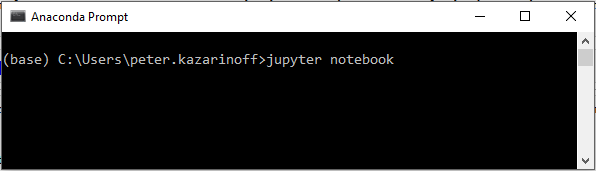
\includegraphics{images/Anaconda_Prompt_Jupyter_Notebook.png}
\caption{Anaconda Prompt Jupyter Notebook}
\end{figure}

A webbrowser will open and something which looks kind of like a file
browser will be shown:

\begin{figure}
\centering
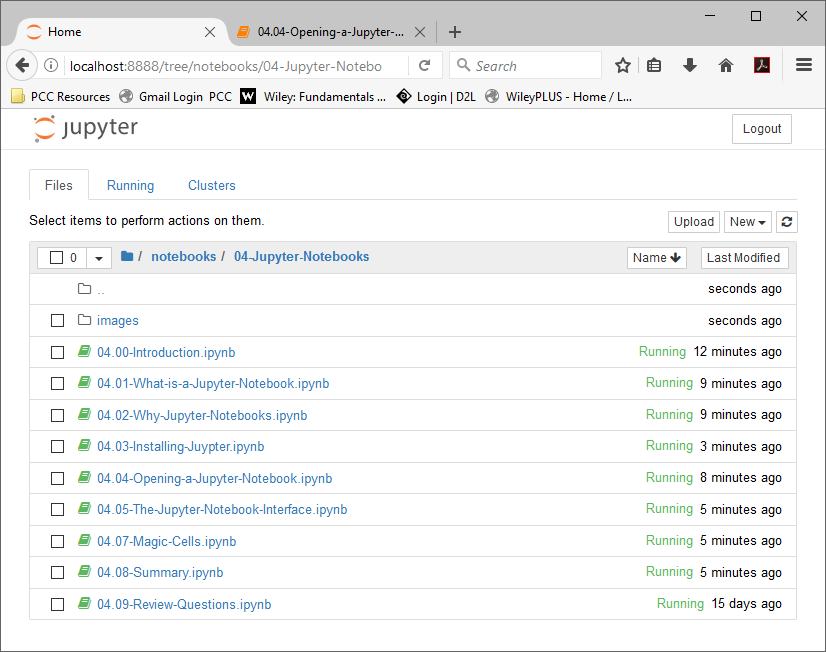
\includegraphics{images/Jupyter_Home_Browser.png}
\caption{Jupyter File Browser}
\end{figure}

Here you can select an exhisting jupyter notebook file which will end
with the \lstinline!.ipynb! extension (which stands for IPython
Notebook). You can also start a new Jupyter Notebook my clicking the
{[}New{]} button in the upper right and selecting {[}Python 3{]}
    




    
        \section{The Jupyter Notebook
Interface}\label{the-jupyter-notebook-interface}

When a new notebook opens, you will see the Jupter Notebook interface.
Accross the top of the notebook will the the Jupyter icon and the
Notebook name. You can click in the notebook name field and change the
name of the notebook. Note that the file extension \lstinline!.ipynb! is
not printed in the file name field, but if you look in the Home tab, you
will see that the notebook is saved with the \lstinline!.ipynb!
extension.
    




    
        \subsection{Menus and Buttons}\label{menus-and-buttons}

A jupyter notebook is comprised of a bunch of cells which are arrayed
one after another in boxes below the menu items and buttons. There are
two main types of cells: Markdown cells and Code cells.
    




    
        \subsection{Code Cells}\label{code-cells}

In code cells you can type Python Code and see the output. An example of
a code cell is shown below. Note that the code cell has an the text
\lstinline!In[ ]! to the left of it.

To run the code in a code cell push the {[}Run{]} button or type
{[}Shift{]}+{[}Enter{]}
    




    
        \subsection{Markdown Cells}\label{markdown-cells}

In markdown cells you can type text and headings. Markdown cells are
used for documentation and explaining your code. The text in a markdown
cell is not executed. Markdown cells can be formatted with a few special
characters

\subsubsection{Headings}\label{headings}

\begin{lstlisting}
# H1 Heading
\end{lstlisting}

\begin{lstlisting}
## H2 Heading
\end{lstlisting}

\begin{lstlisting}
### H3 Heading
\end{lstlisting}

\begin{lstlisting}
#### H4 Heading
\end{lstlisting}

\subsubsection{Code Blocks}\label{code-blocks}

For inline code blocks use the ` left quote character, the character to
the left of the number 1 and above tab on most keyboards.

This is inline code: ` ` ` Inline code block ` ` ` within a paragraph

For seperate code blocks use three ` left quote characters on one line,
followed by the code block on seperate lines. Terminate the seperate
code block with a line of three ` left quote characters.

```

Seperated code blocks

```

\subsubsection{Bold and italics}\label{bold-and-italics}

\textbf{Bold} and \emph{italic font} is diplayed by surrounding text
with a double asterisk for \lstinline!**bold**! and a single underscore
for \lstinline!_italics_!

\lstinline!**bold**! produces \textbf{bold}

\lstinline!_italics_! produces \emph{italics}

\lstinline!**_bold and italic_**! produces \textbf{\emph{bold and
italic}}

\subsubsection{Tables}\label{tables}

Tables are displayed using the pipe \lstinline!|! character, which is
{[}Shift{]}+{[}\textbackslash{}{]} on most keyboards. Columns are
seperated by pipes and rows are seperated by lines. After the header
row, a row of pipes and dashes are needed to define the table.

\begin{lstlisting}
| header1 | header 2 | header 3 |
| --- | --- | --- |
| col 1 | col 2 | col 3 |
| col 1 | col 2 | col 3 |
\end{lstlisting}

produces:

\begin{longtable}[]{@{}lll@{}}
\toprule
header1 & header 2 & header 3\tabularnewline
\midrule
\endhead
col 1 & col 2 & col 3\tabularnewline
col 1 & col 2 & col 3\tabularnewline
\bottomrule
\end{longtable}

\subsubsection{Bullet Points and Lists}\label{bullet-points-and-lists}

Bullet points are produced using the asterisk character \lstinline!*!

\begin{lstlisting}
 * item 1
 * item 2
 * item 3
\end{lstlisting}

produces

\begin{itemize}
\tightlist
\item
  item 1
\item
  item 2
\end{itemize}

Numbered lists are produced using sequential numbers followed by a dot.
Indent sub-items with two spaces.

\begin{lstlisting}
1. First item
2. Second item
3. Third item
  1. sub item
  2. sub item
    1. sub-sub item
    2. sub-sub item
\end{lstlisting}

produces

\begin{enumerate}
\def\labelenumi{\arabic{enumi}.}
\tightlist
\item
  First item
\item
  Second item
\item
  Third item
\item
  sub item
\item
  sub item

  \begin{enumerate}
  \def\labelenumii{\arabic{enumii}.}
  \tightlist
  \item
    sub-sub item
  \item
    sub-sub item
  \end{enumerate}
\end{enumerate}

\subsubsection{Horizontal Rule}\label{horizontal-rule}

A horizontal rule is specified with three asterisks on a single line.

\begin{lstlisting}
***
\end{lstlisting}

produces

\begin{center}\rule{0.5\linewidth}{\linethickness}\end{center}

\subsubsection{Links}\label{links}

Hyperlinks are specified using a set of square brackets \lstinline![ ]!
followed by pair of parenthesis \lstinline!( )! The text inside the
square brackets will be the link, the link address goes in the
parenthesis

\begin{lstlisting}
[link to docs](https://docs.python.org/3/)
\end{lstlisting}

produces

\href{https://docs.python.org/3/}{link to docs}

\subsubsection{Images}\label{images}

Images are embedded in Jupyter Notebook markdown using the exclaimation
point and square brackets \lstinline"![ ]", followed by the image file
path in parenthesis \lstinline!( )!. If the image can not be displayed,
the text in square brackets will be shown. The image can be in the same
directory as the notebook, or a relative path can be specified. In this
case the image \lstinline!engineering.png! is stored in the images
directory, which is a subdirectory of the directory the notebook is
saved in.

\begin{lstlisting}
![Python Logo](images/engineering.png)
\end{lstlisting}

produces

\begin{figure}
\centering

\includegraphics{images/engineering.png}
\caption{Python Logo}
\end{figure}

\subsubsection{LaTeX Math}\label{latex-math}

LaTeX Math equations and symbols are rendered by markdown cells. A more
extensive list of LaTeX commands can be found in the appendix.

\begin{lstlisting}
$$ \int_{a}^{b} \frac{1}{x^2} dx $$
\end{lstlisting}

produces

\[ \int_{a}^{b} \frac{1}{x^2} dx \]

\subsubsection{html}\label{html}

Because jupyter notebooks are rendered by web browsers, just about any
html tag can be included in the markdown portion of a notebook. An
example is the \lstinline!<sup>! \lstinline!</sup>! tags that surround
super script text

\begin{lstlisting}
x<sup>2</sup>
\end{lstlisting}

produces

x2

Text can be colored using html \lstinline!<font>! \lstinline!</font>!
tags

\begin{lstlisting}
<font color=red>Red Text</font>
\end{lstlisting}

produces

Red Text

\subsubsection{warning boxes}\label{warning-boxes}

bootstrap style warning boxes can be included in jupyter notebook
markdown using \lstinline!<div>! tags

\begin{lstlisting}
<div class="alert alert-danger" role="alert">
  <strong>Warning!</strong> Python lists start at 0
</div>
\end{lstlisting}

produces

Warning! Python lists start at 0
    




    
        \subsection{Saving Jupyter Notebooks in Other
Formats}\label{saving-jupyter-notebooks-in-other-formats}

Jupyter notebooks can be saved in other formats besides the native
\lstinline!.ipynb! format. These formats can be acceed on the {[}File{]}
--\textgreater{} {[}Download As{]} menu.

\begin{figure}
\centering
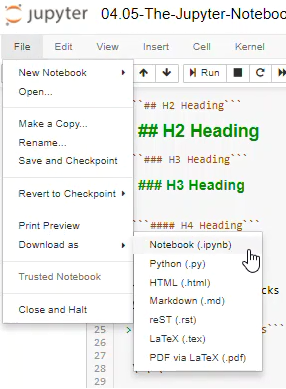
\includegraphics{images/jupyter_notebook_export_options.png}
\caption{Jupyter Notebook Export Optinos}
\end{figure}

The available file types are:

\begin{itemize}
\tightlist
\item
  Notebook (.ipynb) - The native jupyter notebook format
\item
  Python (.py) - The native Python code file type.
\item
  HTML (.html) - A web page
\item
  Markdown (.md) - Markdown format
\item
  reST (.rst) - Restructured text format
\item
  LaTeX (.tex) - LaTeX Artile format
\item
  PDF via LaTeX - a pdf exported from LeTeX, requires a converter
\end{itemize}

When a Notebook is saved as a \lstinline!.py! file, any text in Mardown
Cells are converted to commments, and any code cells are kept as Python
code.

\begin{figure}
\centering
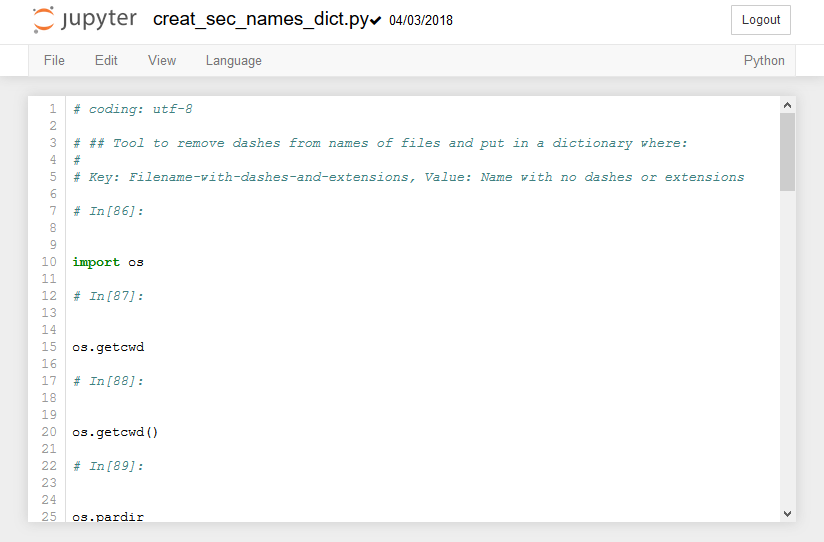
\includegraphics{images/jupyter_notebook_markdown_cells_as_comments.png}
\caption{Markdown Cells as Comments}
\end{figure}

The \lstinline!.py! file after this notebook is
\lstinline!Downloaded as! a \lstinline!Python(.py)! looks like:

\begin{figure}
\centering
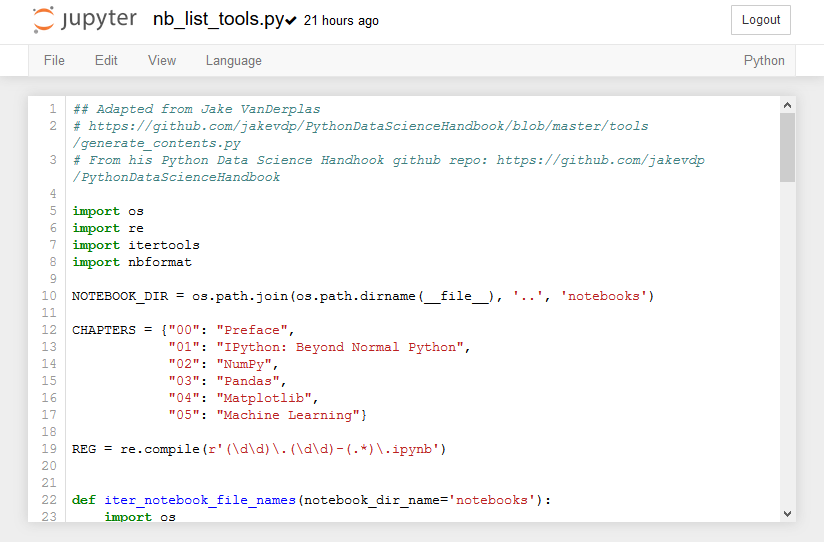
\includegraphics{images/jupyter_notebook_dot_py_file.png}
\caption{Image of Notebook}
\end{figure}
    




    
        \section{Magic Cells}\label{magic-cells}
    




    
        Jupyter notebook code cells can contain special commands which are note
valid Python code, but will affect the behavior of the notebook
    




    
        \subsection{\%matplotlib inline}\label{matplotlib-inline}
    




    
        One of the most popular magic commands is:

\begin{lstlisting}
%matplotlib inline
\end{lstlisting}

Using this command at the top of a jupyter notebook will produce
matplotlib plots in cells of the notebook. Without
\lstinline!%matplotlib inline!, plots will jump out as external windows.
A typical start to a jupyter notebook using \textbf{matplotlib} might
start as:

\begin{lstlisting}
import numpy as np
import pandas as pd
import matplotlib.pyplot as plt
%matplotlib inline
\end{lstlisting}
    




    
        \subsection{\%run}\label{run}
    




    
        The \lstinline!%run! magic command followed by the name of a python file
will run the current python file as a script. Suppose the file
\lstinline!hello.py! is created in the same directory as the running
jupyter notebook. The directory structure will look something like this:

\begin{lstlisting}
| folder
---| notebook.ipynb
---| hello.py
\end{lstlisting}

In the file \lstinline!hello.py! is the code:

\begin{lstlisting}
print('This code was run from a seperate Python file')
print('Hellow from the file hello.py')
\end{lstlisting}

Within our jupyter notebook, if we \lstinline!%run! this file, we will
get the output of or hello.py script in a jupyter notebook output cell.
    



    \begin{Verbatim}[commandchars=\\\{\}]
{\color{incolor}In [{\color{incolor}3}]:} \PY{o}{\PYZpc{}}\PY{k}{run} hello.py
\end{Verbatim}


    \begin{Verbatim}[commandchars=\\\{\}]
This code was run from a seperate Python file
Hellow from the file hello.py

    \end{Verbatim}

    \begin{Verbatim}[commandchars=\\\{\}]
{\color{incolor}In [{\color{incolor}10}]:} \PY{o}{\PYZpc{}}\PY{k}{pwd}
\end{Verbatim}


\begin{Verbatim}[commandchars=\\\{\}]
{\color{outcolor}Out[{\color{outcolor}10}]:} 'C:\textbackslash{}\textbackslash{}Users\textbackslash{}\textbackslash{}peter.kazarinoff\textbackslash{}\textbackslash{}Documents\textbackslash{}\textbackslash{}book\textbackslash{}\textbackslash{}notebooks\textbackslash{}\textbackslash{}04-Jupyter-Notebooks'
\end{Verbatim}
            
    \begin{Verbatim}[commandchars=\\\{\}]
{\color{incolor}In [{\color{incolor}11}]:} \PY{o}{\PYZpc{}}\PY{k}{ls}
\end{Verbatim}


    \begin{Verbatim}[commandchars=\\\{\}]
 Volume in drive C is Windows
 Volume Serial Number is A048-4C53

 Directory of C:\textbackslash{}Users\textbackslash{}peter.kazarinoff\textbackslash{}Documents\textbackslash{}book\textbackslash{}notebooks\textbackslash{}04-Jupyter-Notebooks

04/19/2018  06:01 PM    <DIR>          .
04/19/2018  06:01 PM    <DIR>          ..
04/18/2018  12:24 PM    <DIR>          .ipynb\_checkpoints
04/18/2018  12:17 PM             1,164 04.00-Introduction.ipynb
04/18/2018  12:21 PM             1,125 04.01-What-is-a-Jupyter-Notebook.ipynb
04/18/2018  12:21 PM             1,477 04.02-Why-Jupyter-Notebooks.ipynb
04/18/2018  12:26 PM             1,901 04.03-Installing-Juypter.ipynb
04/18/2018  02:37 PM             2,029 04.04-Opening-a-Jupyter-Notebook.ipynb
04/19/2018  07:23 AM             4,196 04.05-The-Jupyter-Notebook-Interface.ipynb
04/19/2018  06:01 PM            11,102 04.07-Magic-Cells.ipynb
04/18/2018  12:24 PM             1,325 04.08-Summary.ipynb
04/03/2018  04:11 PM               970 04.09-Review-Questions.ipynb
04/19/2018  05:53 PM                94 hello.py
04/18/2018  02:36 PM    <DIR>          images
              10 File(s)         25,383 bytes
               4 Dir(s)  133,241,610,240 bytes free

    \end{Verbatim}


    
        \subsection{Other usefull magic
commands}\label{other-usefull-magic-commands}
    




    
        Other usefull magic commands are:

\begin{longtable}[]{@{}ll@{}}
\toprule
magic command & result\tabularnewline
\midrule
\endhead
\%pwd & print the current working directory\tabularnewline
\%cd & change the current working directory\tabularnewline
\%ls & list the contents of the current directory\tabularnewline
\%history & the history of the \lstinline!In [ ]:!
commands\tabularnewline
\bottomrule
\end{longtable}

You can list all of the available magic commands by typing and running
\lstinline!%lsmagic! in a jupyter notebook code cell:
    



    \begin{Verbatim}[commandchars=\\\{\}]
{\color{incolor}In [{\color{incolor}12}]:} \PY{o}{\PYZpc{}}\PY{k}{lsmagic}
\end{Verbatim}


\begin{Verbatim}[commandchars=\\\{\}]
{\color{outcolor}Out[{\color{outcolor}12}]:} Available line magics:
         \%alias  \%alias\_magic  \%autocall  \%automagic  \%autosave  \%bookmark  \%cd  \%clear  \%cls  \%colors  \%config  \%connect\_info  \%copy  \%ddir  \%debug  \%dhist  \%dirs  \%doctest\_mode  \%echo  \%ed  \%edit  \%env  \%gui  \%hist  \%history  \%killbgscripts  \%ldir  \%less  \%load  \%load\_ext  \%loadpy  \%logoff  \%logon  \%logstart  \%logstate  \%logstop  \%ls  \%lsmagic  \%macro  \%magic  \%matplotlib  \%mkdir  \%more  \%notebook  \%page  \%pastebin  \%pdb  \%pdef  \%pdoc  \%pfile  \%pinfo  \%pinfo2  \%popd  \%pprint  \%precision  \%profile  \%prun  \%psearch  \%psource  \%pushd  \%pwd  \%pycat  \%pylab  \%qtconsole  \%quickref  \%recall  \%rehashx  \%reload\_ext  \%ren  \%rep  \%rerun  \%reset  \%reset\_selective  \%rmdir  \%run  \%save  \%sc  \%set\_env  \%store  \%sx  \%system  \%tb  \%time  \%timeit  \%unalias  \%unload\_ext  \%who  \%who\_ls  \%whos  \%xdel  \%xmode
         
         Available cell magics:
         \%\%!  \%\%HTML  \%\%SVG  \%\%bash  \%\%capture  \%\%cmd  \%\%debug  \%\%file  \%\%html  \%\%javascript  \%\%js  \%\%latex  \%\%perl  \%\%prun  \%\%pypy  \%\%python  \%\%python2  \%\%python3  \%\%ruby  \%\%script  \%\%sh  \%\%svg  \%\%sx  \%\%system  \%\%time  \%\%timeit  \%\%writefile
         
         Automagic is ON, \% prefix IS NOT needed for line magics.
\end{Verbatim}
            

    
        \newpage
        \section{Summary}\label{summary}

    




    
        In this chapter we learned\ldots{}
    




    
        \subsection{Key Terms and Concepts}\label{key-terms-and-concepts}
    




    
        Kernal

Notebook

Jupyter

iPython

Execute

.ipynb file

backend
    




    
        \subsection{Python Commands and
Functions}\label{python-commands-and-functions}
    




    
        \subsubsection{Jupyter Notebook Magic
Commands}\label{jupyter-notebook-magic-commands}

\begin{longtable}[]{@{}ll@{}}
\toprule
Command & Description\tabularnewline
\midrule
\endhead
\lstinline!%matplotlib inline! & Display plots in output
cells\tabularnewline
\lstinline!%run file.py! & Runs file.py and displays
output\tabularnewline
\lstinline!%pwd! & Prints the working directory file path\tabularnewline
\lstinline!%ls! & List contents of the current working
directory\tabularnewline
\lstinline!%precision! & sets float point precision for pretty
printing\tabularnewline
\lstinline!%whos! & lists variables and types in the running kernel
session\tabularnewline
\lstinline!function?! & Display help on a function\tabularnewline
\lstinline!function??! & Display source code of a
function\tabularnewline
\bottomrule
\end{longtable}
    




    
        \section{Review Questions}\label{review-questions}
    




    
        \begin{problems}
        \begin{enumerate}
\def\labelenumi{\arabic{enumi}.}
\item
\item
\item
\item
\item
\item
\item
\item
\end{enumerate}
        \end{problems}

    




    
        \chapter{Functions and Modules}\label{functions-and-modules}
    




    
        \section{Introduction}\label{introduction}
    




    
        By the end of this chapter you will be able to:

\begin{lstlisting}
* import functions and use them in scripts

* create your own functions 

* run functions from other files in your scripts

* create functions with defaut arguments

* provide reusable code for other engineers to use
\end{lstlisting}
        \newpage



    




    
        \section{Why Functions?}\label{why-functions}
    




    
        Functions are reusable pieces of code. Functions are an essention part
of most programming languages. Functions provide a couple of benefits:

\begin{itemize}
\item
  Functions allow the same peice of code to be run multiple times
\item
  Functions can break a long program up into smaller pieces
\item
  Functions can be shared with other programmers
\end{itemize}
    




    
        \section{First Function}\label{first-function}
    




    
        For our first function will create a simple function that adds two to
any number. Functions in Python typically contain at least two lines.
The first line defines the function name and arguments.

\begin{lstlisting}
def function_name(arguments):
    <code>
    return output
\end{lstlisting}

This line contains a couple parts:

\begin{lstlisting}
def
\end{lstlisting}

The key word \lstinline!def! needs to be the start of the line that
declares the function. Def stands for \emph{definition} and indicates to
the Python interpreter that a function definition will follow.

\begin{lstlisting}
function_name
\end{lstlisting}

Each function needs a name. The function name should start with a letter
and is typically all lowercase (in Python names that start with
Uppercase are usually used to define \emph{Classes}). Function names
need to start with a letter and can only contain letters, numbers and
the underscore character. Just about any name will do, but it is best to
avoid using any Python key words such as \lstinline!def!,
\lstinline!class!, \lstinline!if!, \lstinline!else!, \lstinline!for!. A
complete list of reserved Python keywords is in the index.

\begin{lstlisting}
(argument):
\end{lstlisting}

Function names are followed by a set of parenthesis \lstinline!( )!.
Many functions have variable names, called \emph{arguments} in between
the parenthesis. The name used for the function argument should be used
in the body of the function and is only local to that function. After
the parenthesis comes a \lstinline!:! colon. A colon is required to end
the first line of a function.

A colon : is required at the end of the first line of every function. If
the : is not present the code will not run.

\begin{lstlisting}
<code>
\end{lstlisting}

The body of the fuction contains the code that will run when the
function is called. Any variables declared by the function arguments can
be used in the body of the fuction. Any variables used in the body of
the function are \emph{local variables}. Local variables can not be
called or accessed by other scripts.

\begin{lstlisting}
return
\end{lstlisting}

The \lstinline!return! key word is often the last line of a function.
\lstinline!return! indicates that whatever expression that follows will
be the output of the function. The \lstinline!return! keyword is not a
function or a method and parenthesis are not used after
\lstinline!return!, just a space

\begin{lstlisting}
output
\end{lstlisting}

Whatever expression is included after \lstinline!return! will be
\emph{returned} or outputted by the function. The output expression
after \lstinline!return! can be a single variable, value or be a more
complex expression that includes multiple variables.
    




    
        A simple first function, is a function that will add two to any number.
The function will be called \lstinline!plustwo! and have one input
argument, a number. The function will return that number plus
\lstinline!2!. So the function should operate as shown below:

\begin{lstlisting}
plustwo(3)
5
\end{lstlisting}
    



    \begin{Verbatim}[commandchars=\\\{\}]
{\color{incolor}In [{\color{incolor}1}]:} \PY{k}{def} \PY{n+nf}{plustwo}\PY{p}{(}\PY{n}{n}\PY{p}{)}\PY{p}{:}
            \PY{n}{n} \PY{o}{=} \PY{n}{n} \PY{o}{+} \PY{l+m+mi}{2}
            \PY{k}{return} \PY{n}{n}
\end{Verbatim}


    \begin{Verbatim}[commandchars=\\\{\}]
{\color{incolor}In [{\color{incolor}2}]:} \PY{n}{plustwo}\PY{p}{(}\PY{l+m+mi}{3}\PY{p}{)}
\end{Verbatim}


\begin{Verbatim}[commandchars=\\\{\}]
{\color{outcolor}Out[{\color{outcolor}2}]:} 5
\end{Verbatim}
            
    \begin{Verbatim}[commandchars=\\\{\}]
{\color{incolor}In [{\color{incolor}3}]:} \PY{n}{plustwo}\PY{p}{(}\PY{l+m+mi}{10}\PY{p}{)}
\end{Verbatim}


\begin{Verbatim}[commandchars=\\\{\}]
{\color{outcolor}Out[{\color{outcolor}3}]:} 12
\end{Verbatim}
            

    
        \section{Functions with Multiple
Arguments}\label{functions-with-multiple-arguments}
    




    
        Functions can be written to accept multiple arguments. When multiple
arguments are specified, they are listed within the parenthesis after
the fuction name and seperated by a comma:

\begin{lstlisting}
def function_name(argument1, argument2):
    <code>
    return output
\end{lstlisting}

An example function that adds that finds the area of a triangle given
the base and height would accept two arguments \lstinline!base! and
\lstinline!height!.
    



    \begin{Verbatim}[commandchars=\\\{\}]
{\color{incolor}In [{\color{incolor}4}]:} \PY{k}{def} \PY{n+nf}{triarea}\PY{p}{(}\PY{n}{base}\PY{p}{,} \PY{n}{height}\PY{p}{)}\PY{p}{:}
            \PY{n}{area} \PY{o}{=} \PY{l+m+mf}{0.5} \PY{o}{*} \PY{n}{base} \PY{o}{*} \PY{n}{height}
            \PY{k}{return} \PY{n}{area}
\end{Verbatim}


    \begin{Verbatim}[commandchars=\\\{\}]
{\color{incolor}In [{\color{incolor}3}]:} \PY{n}{triarea}\PY{p}{(}\PY{l+m+mi}{10}\PY{p}{,}\PY{l+m+mi}{5}\PY{p}{)}
\end{Verbatim}


\begin{Verbatim}[commandchars=\\\{\}]
{\color{outcolor}Out[{\color{outcolor}3}]:} 25.0
\end{Verbatim}
            

    
        \section{Functions with Default
Arguments}\label{functions-with-default-arguments}
    




    
        Functions can be specified with default arguemnts. If values for these
arguemnts are not supplied when the fuction is called, the default
values will be used. The general format is below:

\begin{lstlisting}
def function_name(arugment1=default_value, arguemnt2=default_value):
    <code>
    return output
\end{lstlisting}
    




    
        An example function is one that calculates the distance an object falls
based on time. The general formula for fall distance \(d\) based on fall
time \(t\) can be modeled as:

\[ d = \frac{1}{2}gt^2 \]

Where \(g\) is the accelleration due to gravity. On earth the value of
\(g\) is 9.81 m/s2. But on the moon, \(g\) is about 1.625 m/s2. Our
function will include the default value for earth's gravity and give
programmers the option of specifying a different value for \(g\) if they
choose.
    



    \begin{Verbatim}[commandchars=\\\{\}]
{\color{incolor}In [{\color{incolor}5}]:} \PY{k}{def} \PY{n+nf}{falldist}\PY{p}{(}\PY{n}{t}\PY{p}{,} \PY{n}{g}\PY{o}{=}\PY{l+m+mf}{9.81}\PY{p}{)}\PY{p}{:}
            \PY{n}{d} \PY{o}{=} \PY{l+m+mf}{0.5} \PY{o}{*} \PY{n}{g} \PY{o}{*} \PY{n}{t}\PY{o}{*}\PY{o}{*}\PY{l+m+mi}{2}
            \PY{k}{return} \PY{n}{d}
\end{Verbatim}



    
        On earth, a ball that falls for three seconds, can be calculated using
\lstinline!falldist(3)! and leaving out a value for \lstinline!g!.
    



    \begin{Verbatim}[commandchars=\\\{\}]
{\color{incolor}In [{\color{incolor}6}]:} \PY{n}{falldist}\PY{p}{(}\PY{l+m+mi}{3}\PY{p}{)}
\end{Verbatim}


\begin{Verbatim}[commandchars=\\\{\}]
{\color{outcolor}Out[{\color{outcolor}6}]:} 44.145
\end{Verbatim}
            

    
        On the moon, gravity is much weaker, an acceleration of 1.625 m/s2. To
calculate how far a ball falls on the moon in three seconds, two
arguments need to be supplied \lstinline!3! and \lstinline!1.625!. If a
second argument is given, this overrides the default value assigned in
the first line of the function.
    



    \begin{Verbatim}[commandchars=\\\{\}]
{\color{incolor}In [{\color{incolor}8}]:} \PY{n}{falldist}\PY{p}{(}\PY{l+m+mi}{3}\PY{p}{,} \PY{l+m+mf}{1.625}\PY{p}{)}
\end{Verbatim}


\begin{Verbatim}[commandchars=\\\{\}]
{\color{outcolor}Out[{\color{outcolor}8}]:} 7.3125
\end{Verbatim}
            

    
        \section{Calling Functions from Other
Files}\label{calling-functions-from-other-files}
    




    
        User-defined functions can be called from other files. A function can be
called and run in a different file than the file the function definition
is written in. If a new file called \textbf{\emph{myfunctions.py}} is
created and contains two function definitions, \lstinline!plustwo()! and
\lstinline!falldist()!, these functions can be used by a separate file
as long as the file and function names are imported first. It is
important that the file which contains the functions ends in the
\textbf{\emph{.py}} extension. Without a \textbf{\emph{.py}} extension,
the file can not be imported.
    




    
        Inside the file \textbf{\emph{myfuctions.py}}, two functions are defined
using the code below.

\begin{lstlisting}[language=Python]
# myfunctions.py

def plustwo(n):
    n = n + 2
    return n


def falldist(t,g=9.81):
    d = 0.5 * g * t**2
    return d
\end{lstlisting}
    




    
        This file, \textbf{\emph{myfunctions.py}} can be imported into another
script (another \textbf{.py} file), or Jupyter Notebook. Remember though
that the file with the functions and the file calling the functions must
be in the same directory. To use the functions written in one file
inside another file include the import line,
\lstinline!from <filename> import <function_name>!. Note that although
the file name must contain a \textbf{\emph{.py}} extension,
\lstinline!.py! is not used as part of the file name during import.
    



    \begin{Verbatim}[commandchars=\\\{\}]
{\color{incolor}In [{\color{incolor}1}]:} \PY{k+kn}{from} \PY{n+nn}{myfunctions} \PY{k}{import} \PY{n}{plustwo}
        \PY{n}{plustwo}\PY{p}{(}\PY{l+m+mi}{3}\PY{p}{)}
\end{Verbatim}


\begin{Verbatim}[commandchars=\\\{\}]
{\color{outcolor}Out[{\color{outcolor}1}]:} 5
\end{Verbatim}
            
    \begin{Verbatim}[commandchars=\\\{\}]
{\color{incolor}In [{\color{incolor}2}]:} \PY{k+kn}{from} \PY{n+nn}{myfunctions} \PY{k}{import} \PY{n}{falldist}
        \PY{n}{falldist}\PY{p}{(}\PY{l+m+mi}{3}\PY{p}{)}
\end{Verbatim}


\begin{Verbatim}[commandchars=\\\{\}]
{\color{outcolor}Out[{\color{outcolor}2}]:} 44.145
\end{Verbatim}
            

    
        \section{Docstrings in Functions}\label{docstrings-in-functions}
    




    
        It is good programming practice to document your code. Reusable chunks
of code are particulary important to document as other programmers may
use the code and you may use the code again at a different time.

Python has a couple different ways for programmers to add documentation.
One way is to use simple comments. Comments are lines of code that do
not get run by the Python interpreter. Comments are meant to be viewed
by humans. In Python, comment lines start with the pound symbol
\lstinline!#!. Any line that starts with a \lstinline!#! will not be run
by the Python Python Interpreter.

Another way to document code is to use \emph{docstrings}. Docstrings are
comments which are surrounded with triple quotation marks and usually
contain multiple lines of explanation. A function containing a docstring
takes the form:

\begin{lstlisting}
def function_name(arguments):
    """"
    Docstring text
    
    
    
    """
    <code>
    
    return <output>
    
\end{lstlisting}

Doc strings are what come up when the \lstinline!help()! function is
called. As an example, running the \lstinline!help()! function on the
built-in function \lstinline!sum! brings up:
    



    \begin{Verbatim}[commandchars=\\\{\}]
{\color{incolor}In [{\color{incolor}4}]:} \PY{n}{help}\PY{p}{(}\PY{n+nb}{sum}\PY{p}{)}
\end{Verbatim}


    \begin{Verbatim}[commandchars=\\\{\}]
Help on built-in function sum in module builtins:

sum(iterable, start=0, /)
    Return the sum of a 'start' value (default: 0) plus an iterable of numbers
    
    When the iterable is empty, return the start value.
    This function is intended specifically for use with numeric values and may
    reject non-numeric types.


    \end{Verbatim}


    
        We can produce the same type of output when a user types types
\lstinline!help()! by adding docstrings to a function.
    




    
        Let's create our own function to convert g to kg. Let's call our
function \lstinline!g2kg!. The first thing to do is make sure that the
name \lstinline!g2kg! is not assigned to another function and is not a
keyword by Python. We can check quick using \lstinline!type()!. We know
that \lstinline!sum()! is a function, how about g2kg?
    



    \begin{Verbatim}[commandchars=\\\{\}]
{\color{incolor}In [{\color{incolor}5}]:} \PY{n+nb}{print}\PY{p}{(}\PY{n+nb}{type}\PY{p}{(}\PY{n+nb}{sum}\PY{p}{)}\PY{p}{)}
        \PY{n+nb}{print}\PY{p}{(}\PY{n+nb}{type}\PY{p}{(}\PY{n}{g2kg}\PY{p}{)}\PY{p}{)}
\end{Verbatim}


    \begin{Verbatim}[commandchars=\\\{\}]
<class 'builtin\_function\_or\_method'>

    \end{Verbatim}

    \begin{Verbatim}[commandchars=\\\{\}]

        ------------------------------------------------------------------------

        NameError                              Traceback (most recent call last)

        <ipython-input-5-487fcfc6eb43> in <module>()
          1 print(type(sum))
    ----> 2 print(type(g2kg))
    

        NameError: name 'g2kg' is not defined

    \end{Verbatim}


    
        Since \lstinline!g2kg! is not defined, we can use \lstinline!g2kg! as
the name of a user-defined function. Once we know that our Remember the
parenthsis, colon and return statment.
    



    \begin{Verbatim}[commandchars=\\\{\}]
{\color{incolor}In [{\color{incolor}6}]:} \PY{k}{def} \PY{n+nf}{g2kg}\PY{p}{(}\PY{n}{g}\PY{p}{)}\PY{p}{:}
            \PY{n}{kg} \PY{o}{=} \PY{n}{g}\PY{o}{/}\PY{l+m+mi}{1000}
            
            \PY{k}{return} \PY{n}{kg}
\end{Verbatim}



    
        Now let's try and use our function. How many kg's is 1300 grams. We
expect the output to be 1.3 kg
    



    \begin{Verbatim}[commandchars=\\\{\}]
{\color{incolor}In [{\color{incolor}7}]:} \PY{n}{g2kg}\PY{p}{(}\PY{l+m+mi}{1300}\PY{p}{)}
\end{Verbatim}


\begin{Verbatim}[commandchars=\\\{\}]
{\color{outcolor}Out[{\color{outcolor}7}]:} 1.3
\end{Verbatim}
            

    
        If we call \lstinline!help()! on our function \lstinline!g2kg()!,
nothing is returned. Our \lstinline!g2kg()! function does not contain a
docstring yet.
    



    \begin{Verbatim}[commandchars=\\\{\}]
{\color{incolor}In [{\color{incolor}8}]:} \PY{n}{help}\PY{p}{(}\PY{n}{g2kg}\PY{p}{)}
\end{Verbatim}


    \begin{Verbatim}[commandchars=\\\{\}]
Help on function g2kg in module \_\_main\_\_:

g2kg(g)


    \end{Verbatim}


    
        Now let's add a docstring to the function. Common components of
docstrings include:

\begin{itemize}
\tightlist
\item
  a summary of the function
\item
  the function inputs
\item
  the function outputs
\item
  an example of the function running including the result
\end{itemize}
    



    \begin{Verbatim}[commandchars=\\\{\}]
{\color{incolor}In [{\color{incolor}10}]:} \PY{k}{def} \PY{n+nf}{g2kg}\PY{p}{(}\PY{n}{g}\PY{p}{)}\PY{p}{:}
             \PY{l+s+sd}{\PYZdq{}\PYZdq{}\PYZdq{}}
         \PY{l+s+sd}{    }
         \PY{l+s+sd}{    Function g2kg converts between g and kg}
         \PY{l+s+sd}{    }
         \PY{l+s+sd}{    input: a measurement in grams, int or float}
         \PY{l+s+sd}{    output: measurment in kg, float}
         \PY{l+s+sd}{    }
         \PY{l+s+sd}{    Example:}
         \PY{l+s+sd}{    }
         \PY{l+s+sd}{        \PYZgt{}\PYZgt{}\PYZgt{} g2kg(1300)}
         \PY{l+s+sd}{            }
         \PY{l+s+sd}{            1.3}
         \PY{l+s+sd}{        }
         \PY{l+s+sd}{    \PYZdq{}\PYZdq{}\PYZdq{}}
             \PY{n}{kg} \PY{o}{=} \PY{n}{g}\PY{o}{/}\PY{l+m+mi}{1000}
             
             \PY{k}{return} \PY{n}{kg}
\end{Verbatim}



    
        Now let's ask for \lstinline!help()! on our function and see if the
docstring is printed back.
    



    \begin{Verbatim}[commandchars=\\\{\}]
{\color{incolor}In [{\color{incolor}11}]:} \PY{n}{help}\PY{p}{(}\PY{n}{g2kg}\PY{p}{)}
\end{Verbatim}


    \begin{Verbatim}[commandchars=\\\{\}]
Help on function g2kg in module \_\_main\_\_:

g2kg(g)
    Function g2kg converts between g and kg
    
    input: a measurement in grams, int or float
    output: measurment in kg, float
    
    Example:
    
        >>> g2kg(1300)
            
            1.3


    \end{Verbatim}


    
        \section{Positional and Keyword
Arguments}\label{positional-and-keyword-arguments}
    




    
        Python functions can contain two types of arguments: \emph{positional
arguments} and \emph{keyword arguments}.
    




    
        \subsection{Positional Arguments}\label{positional-arguments}

An \emph{argument} is a variable, value or object passed to a function
or method. \emph{Positional arguments} are arguments that need to be
included when a function is called in the proper position or order. The
first positional argument always needs to be listed first, the second
positional argument needs to be listed second, the third positional
argument listed third etc.

An example of positional arguments can be seen in Python's
\lstinline!complex()! function. This function returns a complex number
with a real term and an imaginary term. The order that numbers are
passed to the complex function determines which number is the real term
and which term is the imaginary term.

If the complex number \lstinline!3 + 5j! needs to be created, the two
positional arguments are the numbers \lstinline!3! and \lstinline!5!.
The \lstinline!3! must be listed first and the \lstinline!5! must be
listed second.
    



    \begin{Verbatim}[commandchars=\\\{\}]
{\color{incolor}In [{\color{incolor}1}]:} \PY{n+nb}{complex}\PY{p}{(}\PY{l+m+mi}{3}\PY{p}{,} \PY{l+m+mi}{5}\PY{p}{)}
\end{Verbatim}


\begin{Verbatim}[commandchars=\\\{\}]
{\color{outcolor}Out[{\color{outcolor}1}]:} (3+5j)
\end{Verbatim}
            

    
        On the other hand, if the complex number \lstinline!5 + 3j! needs to be
created, the \lstinline!5! needs to be listed first and the
\lstinline!3! listed second. Writing the same arguments in a different
order produces a different result.
    



    \begin{Verbatim}[commandchars=\\\{\}]
{\color{incolor}In [{\color{incolor}2}]:} \PY{n+nb}{complex}\PY{p}{(}\PY{l+m+mi}{5}\PY{p}{,} \PY{l+m+mi}{3}\PY{p}{)}
\end{Verbatim}


\begin{Verbatim}[commandchars=\\\{\}]
{\color{outcolor}Out[{\color{outcolor}2}]:} (5+3j)
\end{Verbatim}
            

    
        \subsubsection{Positional Arguments specified an
iterable}\label{positional-arguments-specified-an-iterable}

Positional arguments can also be passed to functions and methods using
an iterable object. Examples of iterable objects include lists, tuples
and sets. The general syntax to use is:

\begin{lstlisting}
function(*iterable)
\end{lstlisting}

Where \lstinline!function! is the name of the function and
\lstinline!iterable! is the name of the iterable preceded by the
ampersand \lstinline!*! character. An example of using a list to pass
positional arguments to the \lstinline!complex()! function is below:
    



    \begin{Verbatim}[commandchars=\\\{\}]
{\color{incolor}In [{\color{incolor}3}]:} \PY{n}{term\PYZus{}list} \PY{o}{=} \PY{p}{[}\PY{l+m+mi}{3}\PY{p}{,} \PY{l+m+mi}{5}\PY{p}{]}
        \PY{n+nb}{complex}\PY{p}{(}\PY{o}{*}\PY{n}{term\PYZus{}list}\PY{p}{)}
\end{Verbatim}


\begin{Verbatim}[commandchars=\\\{\}]
{\color{outcolor}Out[{\color{outcolor}3}]:} (3+5j)
\end{Verbatim}
            

    
        \subsection{Keyword Arguments}\label{keyword-arguments}

A \emph{keyword argument} is an argument passed to a function or a
method which is preceded by a \emph{keyword} and an equals sign the
general form is:

\begin{lstlisting}
function(keyword=value)
\end{lstlisting}

Where \lstinline!function! is the function name, \lstinline!keyword! is
the keyword argument and value is the value or object passed as that
keyword. Python's complex function can also accept two keyword
arguments. The two keyword arguments are \lstinline!real=! and
\lstinline!imag=!. To create the complex number \lstinline!3 + 5j! the,
\lstinline!3! and \lstinline!5! can be passed to the function as the
values assigned to the keyword arguments \lstinline!real=! and
\lstinline!imag=!.
    



    \begin{Verbatim}[commandchars=\\\{\}]
{\color{incolor}In [{\color{incolor}4}]:} \PY{n+nb}{complex}\PY{p}{(}\PY{n}{real}\PY{o}{=}\PY{l+m+mi}{3}\PY{p}{,} \PY{n}{imag}\PY{o}{=}\PY{l+m+mi}{5}\PY{p}{)}
\end{Verbatim}


\begin{Verbatim}[commandchars=\\\{\}]
{\color{outcolor}Out[{\color{outcolor}4}]:} (3+5j)
\end{Verbatim}
            

    
        \subsubsection{Keyword Arguments specified by a
dictionary}\label{keyword-arguments-specified-by-a-dictionary}

Keyword arguments can also be passed to functions and methods using
dictionary. The dictionary used must contain the keywords as keys and
the values as values. The general form is:

\begin{lstlisting}
keyword_dict = {'keyword1': value1, 'keyword2': value2}
function(**keyword_dict)
\end{lstlisting}

Where \lstinline!function! is the name of the function and
\lstinline!keyword_dict! is the name of the dictionary containing
keywords and values preceded by the double ampersand \lstinline!**!
character. Note that the keywords when assigned as keys in a dictionary
must be surounded by quotes \lstinline!' '!. An example of using a
dictionary to pass keyword arguments to the \lstinline!complex()!
function is below:
    



    \begin{Verbatim}[commandchars=\\\{\}]
{\color{incolor}In [{\color{incolor}6}]:} \PY{n}{keyword\PYZus{}dict} \PY{o}{=} \PY{p}{\PYZob{}}\PY{l+s+s1}{\PYZsq{}}\PY{l+s+s1}{real}\PY{l+s+s1}{\PYZsq{}}\PY{p}{:} \PY{l+m+mi}{3}\PY{p}{,} \PY{l+s+s1}{\PYZsq{}}\PY{l+s+s1}{imag}\PY{l+s+s1}{\PYZsq{}}\PY{p}{:} \PY{l+m+mi}{5}\PY{p}{\PYZcb{}}
        \PY{n+nb}{complex}\PY{p}{(}\PY{o}{*}\PY{o}{*}\PY{n}{keyword\PYZus{}dict}\PY{p}{)}
\end{Verbatim}


\begin{Verbatim}[commandchars=\\\{\}]
{\color{outcolor}Out[{\color{outcolor}6}]:} (3+5j)
\end{Verbatim}
            
    \begin{Verbatim}[commandchars=\\\{\}]
{\color{incolor}In [{\color{incolor}14}]:} \PY{k+kn}{import} \PY{n+nn}{typing}
         \PY{n}{typing}\PY{o}{.}\PY{n}{get\PYZus{}type\PYZus{}hints}\PY{p}{(}\PY{p}{)}
\end{Verbatim}


\begin{Verbatim}[commandchars=\\\{\}]
{\color{outcolor}Out[{\color{outcolor}14}]:} \{\}
\end{Verbatim}
            
    \begin{Verbatim}[commandchars=\\\{\}]
{\color{incolor}In [{\color{incolor}15}]:} \PY{k+kn}{import} \PY{n+nn}{sys}
         \PY{n}{sys}\PY{o}{.}\PY{n}{getrefcount}\PY{p}{(}\PY{n}{keyword\PYZus{}dict}\PY{p}{)}
\end{Verbatim}


\begin{Verbatim}[commandchars=\\\{\}]
{\color{outcolor}Out[{\color{outcolor}15}]:} 2
\end{Verbatim}
            

    
        \newpage
        \section{Summary}\label{summary}

    




    
        \subsection{Key Terms and Concepts}\label{key-terms-and-concepts}

function

function definition

arguments

default arguments

positional arguments

keyword arguments

output

doc string

return

.py file

import

\subsection{Python Commands}\label{python-commands}

\begin{longtable}[]{@{}ll@{}}
\toprule
Command & Description\tabularnewline
\midrule
\endhead
\lstinline!def! & define a function\tabularnewline
\lstinline!return! & define the expression or value a function
outputs\tabularnewline
\lstinline!import! & import a module or .py file\tabularnewline
\lstinline!from! & import a function or class from a module or .py
file\tabularnewline
\lstinline!as! & name an alias for a function, method or
class\tabularnewline
\lstinline!"""! & define a doc string\tabularnewline
\bottomrule
\end{longtable}
    




    
        \section{Review Questions}\label{review-questions}
    




    
        \begin{problems}
        \begin{enumerate}
\def\labelenumi{\arabic{enumi}.}
\item
\item
\item
\item
\item
\item
\end{enumerate}
        \end{problems}

    




    
        \chapter{Plotting with Matplotlib}\label{plotting-with-matplotlib}
    




    
        \section{Introduction}\label{introduction}
    




    
        By the end of this chapter you will be able to:

\begin{itemize}
\item
  Import matplotlib into a Python script or jupyter notebook
\item
  Construct line plots with matplotlib
\item
  Construct bar charts with matplotlib
\item
  Add error bars to bar charts
\item
  Plot histograms
\item
  Plot contours
\item
  Construct 3D mesh grid plots
\end{itemize}
        \newpage



    




    
        \section{What is Matplotlib?}\label{what-is-matplotlib}
    




    
        Matplotlib is a popular Python package used to plot data. Matplotlib
started as a project in the early 2000's partly to to use Python to
visualize the electonic signals in the brain of epilepsy patients.
Matplotlib's creator, John D. Hunter was a neurobilogist. He was looking
for way to replicate MATLAB's plotting capability with Python. In
addition to starting matplotlib, Dr.~Hunter was part of the founding
group that created Numfocus. The Numfocus group oversees some major
Python projects including \textbf{matplotlib}, \textbf{numpy},
\textbf{pandas} and \textbf{jupyter}.
    




    
        \subsection{Why use Matplotlib?}\label{why-use-matplotlib}
    




    
        \textbf{Matplotlib} is useful for creating static 2D plots, the kind of
plots included in scientific publications and presentations. Almost any
plot created in Micrsoft Excel can be created with \textbf{matplotlib}.
\textbf{Matplotlib} can also be used to make 3D plots and animations.
    




    
        \section{Installing Matplotlib}\label{installing-matplotlib}
    




    
        Before \textbf{matplotlib's} plotting functions an be used.
\textbf{Matplotlib} needs to be installed. Depending on which
distribution of Python is installed on your machine, the installation
methods are slightly different.
    




    
        \subsection{Installing Matplotlib with the Anaconda
Prompt}\label{installing-matplotlib-with-the-anaconda-prompt}

To install \textbf{matplotlib}, open the \textbf{Anaconda Prompt} and
type:

\begin{lstlisting}
> conda install matplotlib
\end{lstlisting}

Type \lstinline!y! for yes when prompted.
    




    
        \subsection{Installing Matplotlib with
pip}\label{installing-matplotlib-with-pip}
    




    
        To install \textbf{matplotlib} with pip, bring up a terminal window and
type:

\begin{lstlisting}
$ pip install matplotlib
\end{lstlisting}

This will install \textbf{matplotlib} in the current working python
environment.
    




    
        \subsection{Verify the installation}\label{verify-the-installation}
    




    
        To verify that \textbf{matplotlib} is installed try to invoke
\textbf{matplotlib's} version at the Python REPL using the
\lstinline!.__version__! attribute common to most Python packages.
    



    \begin{Verbatim}[commandchars=\\\{\}]
{\color{incolor}In [{\color{incolor}1}]:} \PY{o}{\PYZgt{}\PYZgt{}}\PY{o}{\PYZgt{}} \PY{k+kn}{import} \PY{n+nn}{matplotlib}
        \PY{o}{\PYZgt{}\PYZgt{}}\PY{o}{\PYZgt{}} \PY{n}{matplotlib}\PY{o}{.}\PY{n}{\PYZus{}\PYZus{}version\PYZus{}\PYZus{}}
\end{Verbatim}


\begin{Verbatim}[commandchars=\\\{\}]
{\color{outcolor}Out[{\color{outcolor}1}]:} '2.2.2'
\end{Verbatim}
            

    
        \section{Line Plots}\label{line-plots}
    




    
        Line plots in \textbf{matplotlib} can be created using
\textbf{matplotlib's} \textbf{pyplot} library
    




    
        To build a line plot, first import \textbf{matplotlib}. It is common
convention to import \textbf{matplotlib's} \textbf{pyplot} library as
\lstinline!plt!. The \lstinline!plt! alias will be familiar to other
Python users.

If using a jupyter notebook include the line
\lstinline!%matplotlib inline! command after the imports.
\lstinline!%matplotlib inline! is a jupyter notebook magic command which
causes \textbf{matplotlib} plots to display directly inside jupyter
notebook output cells.
    



    \begin{Verbatim}[commandchars=\\\{\}]
{\color{incolor}In [{\color{incolor}1}]:} \PY{k+kn}{import} \PY{n+nn}{matplotlib}\PY{n+nn}{.}\PY{n+nn}{pyplot} \PY{k}{as} \PY{n+nn}{plt}
        \PY{k+kn}{import} \PY{n+nn}{numpy} \PY{k}{as} \PY{n+nn}{np}
        \PY{c+c1}{\PYZsh{} include if using a jupyter notebook}
        \PY{o}{\PYZpc{}}\PY{k}{matplotlib} inline
\end{Verbatim}


    \begin{Verbatim}[commandchars=\\\{\}]
{\color{incolor}In [{\color{incolor}2}]:} \PY{n}{x} \PY{o}{=} \PY{n}{np}\PY{o}{.}\PY{n}{arange}\PY{p}{(}\PY{l+m+mi}{0}\PY{p}{,} \PY{l+m+mi}{4} \PY{o}{*} \PY{n}{np}\PY{o}{.}\PY{n}{pi}\PY{p}{,} \PY{l+m+mf}{0.1}\PY{p}{)}
        \PY{n}{y} \PY{o}{=} \PY{n}{np}\PY{o}{.}\PY{n}{sin}\PY{p}{(}\PY{n}{x}\PY{p}{)}
\end{Verbatim}


    \begin{Verbatim}[commandchars=\\\{\}]
{\color{incolor}In [{\color{incolor}3}]:} \PY{n}{plt}\PY{o}{.}\PY{n}{plot}\PY{p}{(}\PY{n}{x}\PY{p}{,} \PY{n}{y}\PY{p}{)}
        \PY{n}{plt}\PY{o}{.}\PY{n}{show}\PY{p}{(}\PY{p}{)}
\end{Verbatim}


    \begin{center}
    \adjustimage{max size={0.9\linewidth}{0.9\paperheight}}{combined_files/combined_274_0.png}
    \end{center}
    { \hspace*{\fill} \\}
    

    
        \subsection{Features of a matplotlib
plot}\label{features-of-a-matplotlib-plot}
    




    
        A variety of features on a \textbf{matplotlib} plot can be specified.
The following is a list of commonly specified features:
    




    
        \subsubsection{Line Color, Line Width, Line Style, Line Opacity and
Marker
Options}\label{line-color-line-width-line-style-line-opacity-and-marker-options}

The color, width and style of line in a plot can be specificed. Line
color, line width and line style are included as extra arguments in the
\lstinline!plt.plot()! function call.

\begin{lstlisting}
plt.plot(<x-data>,<y-data>, linewideth=<float or int>, linestyle='<linestyle abbreviation>', color='<color abbreviation>', marker='<marker abbreviation>')
\end{lstlisting}

An example \lstinline!plt.plot()! line including line color, line width
and line style options is:

\begin{lstlisting}
plt.plot(x, y, linewidth=2.0, linestyle='+', color='b', alpha=0.5, marker='o')
\end{lstlisting}

Below is a list of linewidths (many other widths are also available)

\begin{longtable}[]{@{}ll@{}}
\toprule
\lstinline!linewidth=<float or int>! & Line Width\tabularnewline
\midrule
\endhead
0.5 & 0.5 pixels wide\tabularnewline
1 & 1 pixel wide\tabularnewline
1.5 & 1.5 pixels wide\tabularnewline
2 & 2 pixels wide\tabularnewline
3 & 3 pixels wide\tabularnewline
\bottomrule
\end{longtable}

Below is a list of line styles

\begin{longtable}[]{@{}ll@{}}
\toprule
\lstinline!linestyle='<style abbreviation>'! & Line Style\tabularnewline
\midrule
\endhead
\lstinline!'-'! or \lstinline!'solid'! & solid line
(default)\tabularnewline
\lstinline!'--'! or \lstinline!'dashed'! & dashed line\tabularnewline
\lstinline!'-.'! or \lstinline!'dashdot'! & dash-dot line\tabularnewline
\lstinline!':'! or \lstinline!'dotted'! & dotted line\tabularnewline
\lstinline!'None'! or \lstinline!' '! or \lstinline!''! & no
line\tabularnewline
\bottomrule
\end{longtable}

Below is a list of color abbreviations. Note \lstinline!'b'! is used for
blue and \lstinline!'k'! is used for black.

\begin{longtable}[]{@{}ll@{}}
\toprule
\lstinline!color ='<color abbreviation>'! & Color Name\tabularnewline
\midrule
\endhead
\lstinline!'b'! & Blue\tabularnewline
\lstinline!'c'! & Cyan\tabularnewline
\lstinline!'g'! & Green\tabularnewline
\lstinline!'k'! & Black\tabularnewline
\lstinline!'m'! & magenta\tabularnewline
\lstinline!'r'! & Red\tabularnewline
\lstinline!'w'! & White\tabularnewline
\lstinline!'y'! & Yellow\tabularnewline
\bottomrule
\end{longtable}

Below is a list of alpha (opacity) values (any alpha value between 0.0
and 1.0 is possible)

\begin{longtable}[]{@{}ll@{}}
\toprule
\lstinline!alpha = <float or int>! & Opacity\tabularnewline
\midrule
\endhead
\lstinline!0! & transparent\tabularnewline
\lstinline!0.5! & Half transparent\tabularnewline
\lstinline!1.0! & Opaque\tabularnewline
\bottomrule
\end{longtable}

Colors can also be specified in hexadecimal form surrounded by quotation
marks like \lstinline!'#FF69B4'! or in RGBA (red,green,blue,oppacity)
color surronded by parenthesis like \lstinline!(255,182,193,0.5)!.

\begin{longtable}[]{@{}ll@{}}
\toprule
\lstinline!color ='<color abbreviation>'! & Color Format\tabularnewline
\midrule
\endhead
\lstinline!'#FF69B4'! & hexadecimal\tabularnewline
\lstinline!(255,182,193,0.5)! & RGBA\tabularnewline
\bottomrule
\end{longtable}

Below is a list of maker styles

\begin{longtable}[]{@{}ll@{}}
\toprule
\lstinline!marker='<marker abbreviation>'! & Marker Style\tabularnewline
\midrule
\endhead
\lstinline!"."! & point\tabularnewline
\lstinline!","! & one pixel\tabularnewline
\lstinline!"o"! & circle\tabularnewline
\lstinline!"v"! & triangle\_down\tabularnewline
\lstinline!"^"! & triangle\_up\tabularnewline
\lstinline!"8"! & octagon\tabularnewline
\lstinline!"s"! & square\tabularnewline
\lstinline!"p"! & pentagon\tabularnewline
\lstinline!"*"! & star\tabularnewline
\lstinline!"h"! & hexagon 1\tabularnewline
\lstinline!"H"! & hexagon 2\tabularnewline
\lstinline!"+"! & plus\tabularnewline
\lstinline!"P"! & filled plus\tabularnewline
\lstinline!"x"! & x\tabularnewline
\lstinline!"X"! & filled x\tabularnewline
\lstinline!"D"! & diamond\tabularnewline
\lstinline!"d"! & thin diamond\tabularnewline
\bottomrule
\end{longtable}

In addition to \lstinline!marker='<marker style>'!, the color of the
marker edge, the color of the marker face and the size of the marker can
be specificed with:

\lstinline!plt.plot( .... markeredgecolor='<color abbreviation>', markerfacecolor='<color abbreviation>', markersize=<float or int>....)!
    




    
        \subsubsection{Title}\label{title}

The plot title will be shown above the plot. The \lstinline!title()!
command accepts a string as an argument

\begin{lstlisting}
plt.title('My Title')
\end{lstlisting}
    




    
        \subsubsection{x-axis label}\label{x-axis-label}

The x-axis label will be down below the x-axis. The \lstinline!xlabel()!
command accepts a string as an argument.

\begin{lstlisting}
plt.xlabel('My x-axis label')
\end{lstlisting}
    




    
        \subsubsection{y-axis label}\label{y-axis-label}

The y-axis label will be shown to the left of the y-axis. The
\lstinline!ylabel()! command accepts a string as an argument.

\begin{lstlisting}
plt.ylabel('My y-axis label')
\end{lstlisting}
    




    
        \subsubsection{Legend}\label{legend}

The legend will apear within the plot area, in the upper right corner by
default. The \lstinline!legend! command accepts a list of strings and
optionally accepts a \lstinline!loc=! argument to position the legend in
a different location

\begin{lstlisting}
plt.legend(['entry1','entry2'], loc = 0)
\end{lstlisting}

The following are the location codes for legend location. These numbers
need to be placed after \lstinline!loc=! in the \lstinline!plt.legend()!
call.

\begin{longtable}[]{@{}ll@{}}
\toprule
Legend Location & \lstinline!loc = <number>!\tabularnewline
\midrule
\endhead
`best' & 0\tabularnewline
`upper right' & 1\tabularnewline
`upper left' & 2\tabularnewline
`lower left' & 3\tabularnewline
`lower right' & 4\tabularnewline
`right' & 5\tabularnewline
`center left' & 6\tabularnewline
`center right' & 7\tabularnewline
`lower center' & 8\tabularnewline
`upper center' & 9\tabularnewline
`center' & 10\tabularnewline
\bottomrule
\end{longtable}
    




    
        \subsubsection{Grid}\label{grid}

A grid can be shown on the plot using the \lstinline!plt.grid()!
command. By defaut, the grid is turned off. To turn on the grid use:

\begin{lstlisting}
plt.grid(True)
\end{lstlisting}

The only valid options are \lstinline!plt.grid(True)! and
\lstinline!plt.grid(False)!. Note that \lstinline!True! and
\lstinline!False! are capitalized and are not enclosed in quotations.
    




    
        \subsection{Line Plot with specified
features}\label{line-plot-with-specified-features}
    




    
        Line plots with the specified features above are constructed according
to this general outline:

\subsubsection{Imports}\label{imports}

Import matplot.pyplot as plt, as well as any other modules needed to
work with the data. If using a jupyter notebook include
\lstinline!%matplotlib inline! in this section

\subsubsection{Define Data}\label{define-data}

Your plot needs to contain something. This is defined after the imports

\subsubsection{Plot Data including
options}\label{plot-data-including-options}

Use \lstinline!plt.plot()! to plot the data defined above. Note the
\lstinline!plt.plot()! needs to be called before any details are
specified. Otherwise the details have no plot to apply to. Besides the
data, arguments in \lstinline!plt.plot()! call can include: *
\lstinline!linewideth= <float or int>! *
\lstinline!linestyle='<linestyle abbreviation>'! *
\lstinline!color='<color abbreviation>'! *
\lstinline!alpha= <float or int>! *
\lstinline!marker='<marker abbreviation>'! *
\lstinline!markeredgecolor='<color abbreviation>'! *
\lstinline!markerfacecolor='<color abbreviation>'! *
\lstinline!markersize=<float or int>!

\subsubsection{Add plot details}\label{add-plot-details}

Add details such as a title, axis labels, legend and colors. Plot
details to add include:

\begin{itemize}
\tightlist
\item
  \lstinline!plt.title('<title string>')!
\item
  \lstinline!plt.xlabel('<x-axis label string>')!
\item
  \lstinline!plt.ylabel('<y-axis label string>')!
\item
  \lstinline!plt.legend(['list','of','strings'])!
\item
  \lstinline!ptl.grid(<True or False>)!
\item
  \lstinline!plt.xticks([list of tick locations, floats or ints],[list of tick labels, strings]!
\item
  \lstinline!plt.yticks([list of tick locations, floats or ints],[list of tick labels, strings]!
\end{itemize}

\subsubsection{Show the plot}\label{show-the-plot}

Use the \lstinline!plt.show()! command to show the plot. This will cause
the plot to display in a jupyter notebook or pop out as a new window if
using a seperate .py script file. Note that the plt.show() needs to be
called after all of the plot specifications.
    




    
        A section of code following this outline and the resulting plot is shown
below:
    



    \begin{Verbatim}[commandchars=\\\{\}]
{\color{incolor}In [{\color{incolor}4}]:} \PY{c+c1}{\PYZsh{} Imports}
        \PY{k+kn}{import} \PY{n+nn}{numpy} \PY{k}{as} \PY{n+nn}{np}
        \PY{k+kn}{import} \PY{n+nn}{matplotlib}\PY{n+nn}{.}\PY{n+nn}{pyplot} \PY{k}{as} \PY{n+nn}{plt}
        \PY{c+c1}{\PYZsh{} Include if using a jupyter notebook. Remove if using a .py\PYZhy{}file.}
        \PY{o}{\PYZpc{}}\PY{k}{matplotlib} inline
        
        \PY{c+c1}{\PYZsh{} Define Data}
        \PY{n}{x} \PY{o}{=} \PY{n}{np}\PY{o}{.}\PY{n}{arange}\PY{p}{(}\PY{l+m+mi}{0}\PY{p}{,} \PY{l+m+mi}{4} \PY{o}{*} \PY{n}{np}\PY{o}{.}\PY{n}{pi}\PY{p}{,} \PY{l+m+mf}{0.2}\PY{p}{)}
        \PY{n}{y} \PY{o}{=} \PY{n}{np}\PY{o}{.}\PY{n}{sin}\PY{p}{(}\PY{n}{x}\PY{p}{)}
        
        \PY{c+c1}{\PYZsh{} Plot Data including options}
        \PY{n}{plt}\PY{o}{.}\PY{n}{plot}\PY{p}{(}\PY{n}{x}\PY{p}{,} \PY{n}{y}\PY{p}{,}
            \PY{n}{linewidth}\PY{o}{=}\PY{l+m+mf}{0.5}\PY{p}{,}
            \PY{n}{linestyle}\PY{o}{=}\PY{l+s+s1}{\PYZsq{}}\PY{l+s+s1}{\PYZhy{}\PYZhy{}}\PY{l+s+s1}{\PYZsq{}}\PY{p}{,}
            \PY{n}{color}\PY{o}{=}\PY{l+s+s1}{\PYZsq{}}\PY{l+s+s1}{r}\PY{l+s+s1}{\PYZsq{}}\PY{p}{,}
            \PY{n}{marker}\PY{o}{=}\PY{l+s+s1}{\PYZsq{}}\PY{l+s+s1}{o}\PY{l+s+s1}{\PYZsq{}}\PY{p}{,}
            \PY{n}{markersize}\PY{o}{=}\PY{l+m+mi}{10}\PY{p}{,}
            \PY{n}{markerfacecolor}\PY{o}{=}\PY{p}{(}\PY{l+m+mi}{1}\PY{p}{,} \PY{l+m+mi}{0}\PY{p}{,} \PY{l+m+mi}{0}\PY{p}{,} \PY{l+m+mf}{0.1}\PY{p}{)}\PY{p}{)}
        
        \PY{c+c1}{\PYZsh{} Add details}
        \PY{n}{plt}\PY{o}{.}\PY{n}{title}\PY{p}{(}\PY{l+s+s1}{\PYZsq{}}\PY{l+s+s1}{Plot of sin(x) vs x from 0 to 4 pi}\PY{l+s+s1}{\PYZsq{}}\PY{p}{)}
        \PY{n}{plt}\PY{o}{.}\PY{n}{xlabel}\PY{p}{(}\PY{l+s+s1}{\PYZsq{}}\PY{l+s+s1}{x (0 to 4 pi)}\PY{l+s+s1}{\PYZsq{}}\PY{p}{)}
        \PY{n}{plt}\PY{o}{.}\PY{n}{ylabel}\PY{p}{(}\PY{l+s+s1}{\PYZsq{}}\PY{l+s+s1}{sin(x)}\PY{l+s+s1}{\PYZsq{}}\PY{p}{)}
        \PY{n}{plt}\PY{o}{.}\PY{n}{legend}\PY{p}{(}\PY{p}{[}\PY{l+s+s1}{\PYZsq{}}\PY{l+s+s1}{sin(x)}\PY{l+s+s1}{\PYZsq{}}\PY{p}{]}\PY{p}{)}
        \PY{n}{plt}\PY{o}{.}\PY{n}{xticks}\PY{p}{(}
            \PY{n}{np}\PY{o}{.}\PY{n}{arange}\PY{p}{(}\PY{l+m+mi}{0}\PY{p}{,} \PY{l+m+mi}{4} \PY{o}{*} \PY{n}{np}\PY{o}{.}\PY{n}{pi}\PY{p}{,} \PY{n}{np}\PY{o}{.}\PY{n}{pi} \PY{o}{/} \PY{l+m+mi}{2}\PY{p}{)}\PY{p}{,}
            \PY{p}{[}\PY{l+s+s1}{\PYZsq{}}\PY{l+s+s1}{0}\PY{l+s+s1}{\PYZsq{}}\PY{p}{,} \PY{l+s+s1}{\PYZsq{}}\PY{l+s+s1}{\PYZdl{}}\PY{l+s+s1}{\PYZbs{}}\PY{l+s+s1}{pi\PYZdl{}/2}\PY{l+s+s1}{\PYZsq{}}\PY{p}{,} \PY{l+s+s1}{\PYZsq{}}\PY{l+s+s1}{\PYZdl{}}\PY{l+s+s1}{\PYZbs{}}\PY{l+s+s1}{pi\PYZdl{}}\PY{l+s+s1}{\PYZsq{}}\PY{p}{,} \PY{l+s+s1}{\PYZsq{}}\PY{l+s+s1}{\PYZdl{}3}\PY{l+s+s1}{\PYZbs{}}\PY{l+s+s1}{pi/2\PYZdl{}}\PY{l+s+s1}{\PYZsq{}}\PY{p}{,} \PY{l+s+s1}{\PYZsq{}}\PY{l+s+s1}{2\PYZdl{}}\PY{l+s+s1}{\PYZbs{}}\PY{l+s+s1}{pi\PYZdl{}}\PY{l+s+s1}{\PYZsq{}}\PY{p}{,} \PY{l+s+s1}{\PYZsq{}}\PY{l+s+s1}{5\PYZdl{}}\PY{l+s+s1}{\PYZbs{}}\PY{l+s+s1}{pi\PYZdl{}/2}\PY{l+s+s1}{\PYZsq{}}\PY{p}{,} \PY{l+s+s1}{\PYZsq{}}\PY{l+s+s1}{3\PYZdl{}}\PY{l+s+s1}{\PYZbs{}}\PY{l+s+s1}{pi\PYZdl{}}\PY{l+s+s1}{\PYZsq{}}\PY{p}{,} \PY{l+s+s1}{\PYZsq{}}\PY{l+s+s1}{7\PYZdl{}}\PY{l+s+s1}{\PYZbs{}}\PY{l+s+s1}{pi\PYZdl{}/2}\PY{l+s+s1}{\PYZsq{}}\PY{p}{]}\PY{p}{)}
        \PY{n}{plt}\PY{o}{.}\PY{n}{grid}\PY{p}{(}\PY{k+kc}{True}\PY{p}{)}
        
        \PY{c+c1}{\PYZsh{} Show the Plot}
        \PY{n}{plt}\PY{o}{.}\PY{n}{show}\PY{p}{(}\PY{p}{)}
\end{Verbatim}


    \begin{center}
    \adjustimage{max size={0.9\linewidth}{0.9\paperheight}}{combined_files/combined_286_0.png}
    \end{center}
    { \hspace*{\fill} \\}
    

    
        \section{Multi Line Plots}\label{multi-line-plots}
    




    
        Multi-line plots in \textbf{matplotlib} can be created using
\textbf{matplotlib's pyplot} library. This section builds upon the work
in the previous section where a plot with one line was created. This
section will also introduce \textbf{matplotlib's} object oriented
approach to building a plot. The object oriented approach to building
plots will be used for the rest of the chapter.
    




    
        \subsection{\texorpdfstring{\textbf{matplotlib} object-oriented
interface}{matplotlib object-oriented interface}}\label{matplotlib-object-oriented-interface}

An object-oriented plotting interface is an interface where components
of the plot (like the axis, title, lines, markers, etc) are treated as
programmatic \emph{objects} that have \emph{attributes} and
\emph{methods} associated with them. To create a new \emph{object} is
called \emph{instantiation}. Once an object is created, or
\emph{instantiated}, the properties of that object can be modified and
methods can be called on the object. The basic annatomy of a
\textbf{matplotlib} plot includes a couple of layers, each of these
layers is a programming \emph{object}:

\begin{itemize}
\tightlist
\item
  Figure Objects: The bottom layer. Think of the figure layer as the
  figure window which contains the minimize, maximize, close buttons. A
  figure can contain one plot or multiple plots
\item
  Plot Objects: A plot builds on the Figure layer. If there are multiple
  plots, each plot is called a subplot.
\item
  Axis Objects: An axis is added to a Plot layer. Axis can be thought of
  as sets of x and y axis that lines and bars are drawn on. An Axis
  contains daughter attributes like axis labels, tick labels and line
  thickness.
\item
  Data Objects: data points, lines, shapes are plotted on an axis
\end{itemize}
    




    
        To build a figure object, \textbf{matplotlib's}
\lstinline!plt.subplot()! function is used. This functions creates both
a figure \emph{object} and an axis \emph{object}. The
\lstinline!plt.subplot()! function \emph{instantiates} a figure
\emph{object} and \emph{instantiates} an axis object. For now, we we'll
leave the \lstinline!subplot()! arguments blank. By default the
\lstinline!subplot()! function will create a single figure object and a
single axis object. We'll call the figure object \lstinline!fig! and the
axis object \lstinline!ax!. Note these two outputs of the
\lstinline!plt.subplots()! function are separated by a comma.

We have a figure object and axis object, but both of these objects are
without attributes. This produces a blank plot. We can add elements to
the axis object to build a plot. Let's create three \textbf{numpy}
arrays to add to our axis object.

The \textbf{numpy} arrays \lstinline!x!, \lstinline!y!, and
\lstinline!z! can be added to to axis object \lstinline!ax!. We add a
plot attribute (a line) to our axis object \lstinline!ax! using the
object oriented structure \lstinline!<object>.<attribute>!. In this
case, \lstinline!ax! is the object and \lstinline!plot! is the
attribute. The \lstinline!plt.show()! line shows the plot on the screen.
    



    \begin{Verbatim}[commandchars=\\\{\}]
{\color{incolor}In [{\color{incolor}1}]:} \PY{k+kn}{import} \PY{n+nn}{matplotlib}\PY{n+nn}{.}\PY{n+nn}{pyplot} \PY{k}{as} \PY{n+nn}{plt}
        \PY{k+kn}{import} \PY{n+nn}{numpy} \PY{k}{as} \PY{n+nn}{np}
        \PY{o}{\PYZpc{}}\PY{k}{matplotlib} inline
        
        \PY{n}{x} \PY{o}{=} \PY{n}{np}\PY{o}{.}\PY{n}{arange}\PY{p}{(}\PY{l+m+mi}{0}\PY{p}{,}\PY{l+m+mi}{4}\PY{o}{*}\PY{n}{np}\PY{o}{.}\PY{n}{pi}\PY{p}{,}\PY{l+m+mf}{0.1}\PY{p}{)}
        \PY{n}{y} \PY{o}{=} \PY{n}{np}\PY{o}{.}\PY{n}{sin}\PY{p}{(}\PY{n}{x}\PY{p}{)}
        \PY{n}{z} \PY{o}{=} \PY{n}{np}\PY{o}{.}\PY{n}{cos}\PY{p}{(}\PY{n}{x}\PY{p}{)}
        
        \PY{n}{fig}\PY{p}{,} \PY{n}{ax} \PY{o}{=} \PY{n}{plt}\PY{o}{.}\PY{n}{subplots}\PY{p}{(}\PY{p}{)}
        
        \PY{n}{ax}\PY{o}{.}\PY{n}{plot}\PY{p}{(}\PY{n}{x}\PY{p}{,}\PY{n}{y}\PY{p}{)}
        \PY{n}{ax}\PY{o}{.}\PY{n}{plot}\PY{p}{(}\PY{n}{x}\PY{p}{,}\PY{n}{z}\PY{p}{)}
        
        \PY{n}{plt}\PY{o}{.}\PY{n}{show}\PY{p}{(}\PY{p}{)}
\end{Verbatim}


    \begin{center}
    \adjustimage{max size={0.9\linewidth}{0.9\paperheight}}{combined_files/combined_291_0.png}
    \end{center}
    { \hspace*{\fill} \\}
    

    
        The \lstinline!ax! object has many methods and attributes. Two methods
we can run on the \lstinline!ax! object include
\lstinline!ax.set_title()! and \lstinline!ax.legend()!. A couple
daughter objects include \lstinline!ax.xaxis! and \lstinline!ax.yaxis!.
These daughter objects in turn have methods such as
\lstinline!ax.xaxis.set_label_text()! and
\lstinline!ax.yaxis.set_label_text()!.
    



    \begin{Verbatim}[commandchars=\\\{\}]
{\color{incolor}In [{\color{incolor}2}]:} \PY{n}{fig}\PY{p}{,} \PY{n}{ax} \PY{o}{=} \PY{n}{plt}\PY{o}{.}\PY{n}{subplots}\PY{p}{(}\PY{p}{)}
        
        \PY{n}{ax}\PY{o}{.}\PY{n}{plot}\PY{p}{(}\PY{n}{x}\PY{p}{,}\PY{n}{y}\PY{p}{)}
        \PY{n}{ax}\PY{o}{.}\PY{n}{plot}\PY{p}{(}\PY{n}{x}\PY{p}{,}\PY{n}{z}\PY{p}{)}
        
        \PY{n}{ax}\PY{o}{.}\PY{n}{set\PYZus{}title}\PY{p}{(}\PY{l+s+s1}{\PYZsq{}}\PY{l+s+s1}{Two Trig Functions}\PY{l+s+s1}{\PYZsq{}}\PY{p}{)}
        \PY{n}{ax}\PY{o}{.}\PY{n}{legend}\PY{p}{(}\PY{p}{[}\PY{l+s+s1}{\PYZsq{}}\PY{l+s+s1}{sin}\PY{l+s+s1}{\PYZsq{}}\PY{p}{,}\PY{l+s+s1}{\PYZsq{}}\PY{l+s+s1}{cos}\PY{l+s+s1}{\PYZsq{}}\PY{p}{]}\PY{p}{)}
        
        \PY{n}{ax}\PY{o}{.}\PY{n}{xaxis}\PY{o}{.}\PY{n}{set\PYZus{}label\PYZus{}text}\PY{p}{(}\PY{l+s+s1}{\PYZsq{}}\PY{l+s+s1}{Angle \PYZdl{}}\PY{l+s+s1}{\PYZbs{}}\PY{l+s+s1}{Theta\PYZdl{}}\PY{l+s+s1}{\PYZsq{}}\PY{p}{)}
        \PY{n}{ax}\PY{o}{.}\PY{n}{yaxis}\PY{o}{.}\PY{n}{set\PYZus{}label\PYZus{}text}\PY{p}{(}\PY{l+s+s1}{\PYZsq{}}\PY{l+s+s1}{Sine and Cosine}\PY{l+s+s1}{\PYZsq{}}\PY{p}{)}
        
        
        \PY{n}{plt}\PY{o}{.}\PY{n}{show}\PY{p}{(}\PY{p}{)}
\end{Verbatim}


    \begin{center}
    \adjustimage{max size={0.9\linewidth}{0.9\paperheight}}{combined_files/combined_293_0.png}
    \end{center}
    { \hspace*{\fill} \\}
    

    
        \section{Bar Charts and Pie Charts}\label{bar-charts-and-pie-charts}
    




    
        Bar charts and pie charts can be created using \textbf{matplotlib's}
\textbf{pyplot} library.
    




    
        \subsection{Bar Charts}\label{bar-charts}
    




    
        To construct a bar plot using \textbf{matplotlib}, first import
\textbf{matplotlib's} \textbf{pyplot} library. The common alias to use
for \lstinline!matplotlib.pyplot! is \lstinline!plt!. If using a Jupiter
notebook include the line \lstinline!%matplotlib inline!.
    



    \begin{Verbatim}[commandchars=\\\{\}]
{\color{incolor}In [{\color{incolor}1}]:} \PY{k+kn}{import} \PY{n+nn}{matplotlib}\PY{n+nn}{.}\PY{n+nn}{pyplot} \PY{k}{as} \PY{n+nn}{plt}
        \PY{k+kn}{import} \PY{n+nn}{numpy} \PY{k}{as} \PY{n+nn}{np}
        \PY{o}{\PYZpc{}}\PY{k}{matplotlib} inline
\end{Verbatim}



    
        We need some data to plot to create a bar chart. In this case, the data
is from a set of \textbf{coefficient of thermal expansion} lab
measurements. The \textbf{coefficient of thermal expansion} (CTE) is a
material property that describes how much a material will change in
length as a result of a change in temperature. Different materials have
different CTE's and we can use the lab data to determine which material
will expand the most if all three are heated up to the same temperature
(assuming all three start at the same temperature).

First, we need to input the data as \textbf{numpy} arrays:
    



    \begin{Verbatim}[commandchars=\\\{\}]
{\color{incolor}In [{\color{incolor}2}]:} \PY{c+c1}{\PYZsh{} Data}
        \PY{n}{aluminum} \PY{o}{=} \PY{n}{np}\PY{o}{.}\PY{n}{array}\PY{p}{(}\PY{p}{[}
            \PY{l+m+mf}{6.4e\PYZhy{}5}\PY{p}{,} \PY{l+m+mf}{3.01e\PYZhy{}5}\PY{p}{,} \PY{l+m+mf}{2.36e\PYZhy{}5}\PY{p}{,} \PY{l+m+mf}{3.0e\PYZhy{}5}\PY{p}{,} \PY{l+m+mf}{7.0e\PYZhy{}5}\PY{p}{,} \PY{l+m+mf}{4.5e\PYZhy{}5}\PY{p}{,} \PY{l+m+mf}{3.8e\PYZhy{}5}\PY{p}{,} \PY{l+m+mf}{4.2e\PYZhy{}5}\PY{p}{,} \PY{l+m+mf}{2.62e\PYZhy{}5}\PY{p}{,}
            \PY{l+m+mf}{3.6e\PYZhy{}5}
        \PY{p}{]}\PY{p}{)}
        \PY{n}{copper} \PY{o}{=} \PY{n}{np}\PY{o}{.}\PY{n}{array}\PY{p}{(}\PY{p}{[}
            \PY{l+m+mf}{4.5e\PYZhy{}5}\PY{p}{,} \PY{l+m+mf}{1.97e\PYZhy{}5}\PY{p}{,} \PY{l+m+mf}{1.6e\PYZhy{}5}\PY{p}{,} \PY{l+m+mf}{1.97e\PYZhy{}5}\PY{p}{,} \PY{l+m+mf}{4.0e\PYZhy{}5}\PY{p}{,} \PY{l+m+mf}{2.4e\PYZhy{}5}\PY{p}{,} \PY{l+m+mf}{1.9e\PYZhy{}5}\PY{p}{,} \PY{l+m+mf}{2.41e\PYZhy{}5}\PY{p}{,} \PY{l+m+mf}{1.85e\PYZhy{}5}\PY{p}{,}
            \PY{l+m+mf}{3.3e\PYZhy{}5}
        \PY{p}{]}\PY{p}{)}
        \PY{n}{steel} \PY{o}{=} \PY{n}{np}\PY{o}{.}\PY{n}{array}\PY{p}{(}\PY{p}{[}
            \PY{l+m+mf}{3.3e\PYZhy{}5}\PY{p}{,} \PY{l+m+mf}{1.2e\PYZhy{}5}\PY{p}{,} \PY{l+m+mf}{0.9e\PYZhy{}5}\PY{p}{,} \PY{l+m+mf}{1.2e\PYZhy{}5}\PY{p}{,} \PY{l+m+mf}{1.3e\PYZhy{}5}\PY{p}{,} \PY{l+m+mf}{1.6e\PYZhy{}5}\PY{p}{,} \PY{l+m+mf}{1.4e\PYZhy{}5}\PY{p}{,} \PY{l+m+mf}{1.58e\PYZhy{}5}\PY{p}{,} \PY{l+m+mf}{1.32e\PYZhy{}5}\PY{p}{,}
            \PY{l+m+mf}{2.1e\PYZhy{}5}
        \PY{p}{]}\PY{p}{)}
\end{Verbatim}



    
        Next, calculate the average or \textbf{mean} using \textbf{numpy's}
\lstinline!np.mean()! function.
    



    \begin{Verbatim}[commandchars=\\\{\}]
{\color{incolor}In [{\color{incolor}3}]:} \PY{c+c1}{\PYZsh{} Calculate the average}
        \PY{n}{aluminum\PYZus{}mean} \PY{o}{=} \PY{n}{np}\PY{o}{.}\PY{n}{mean}\PY{p}{(}\PY{n}{aluminum}\PY{p}{)}
        \PY{n}{copper\PYZus{}mean} \PY{o}{=} \PY{n}{np}\PY{o}{.}\PY{n}{mean}\PY{p}{(}\PY{n}{copper}\PY{p}{)}
        \PY{n}{steel\PYZus{}mean} \PY{o}{=} \PY{n}{np}\PY{o}{.}\PY{n}{mean}\PY{p}{(}\PY{n}{steel}\PY{p}{)}
\end{Verbatim}



    
        Then build a list of materials and CTE's:
    



    \begin{Verbatim}[commandchars=\\\{\}]
{\color{incolor}In [{\color{incolor}4}]:} \PY{c+c1}{\PYZsh{} Create Arrays for the plot}
        \PY{n}{materials} \PY{o}{=} \PY{p}{[}\PY{l+s+s1}{\PYZsq{}}\PY{l+s+s1}{Aluminum}\PY{l+s+s1}{\PYZsq{}}\PY{p}{,} \PY{l+s+s1}{\PYZsq{}}\PY{l+s+s1}{Copper}\PY{l+s+s1}{\PYZsq{}}\PY{p}{,} \PY{l+s+s1}{\PYZsq{}}\PY{l+s+s1}{Steel}\PY{l+s+s1}{\PYZsq{}}\PY{p}{]}
        \PY{n}{x\PYZus{}pos} \PY{o}{=} \PY{n}{np}\PY{o}{.}\PY{n}{arange}\PY{p}{(}\PY{n+nb}{len}\PY{p}{(}\PY{n}{materials}\PY{p}{)}\PY{p}{)}
        \PY{n}{CTEs} \PY{o}{=} \PY{p}{[}\PY{n}{aluminum\PYZus{}mean}\PY{p}{,} \PY{n}{copper\PYZus{}mean}\PY{p}{,} \PY{n}{steel\PYZus{}mean}\PY{p}{]}
\end{Verbatim}



    
        The \lstinline!materials!, \lstinline!x_pos!, and \lstinline!CTEs! (the
labels below the bars) are defined, now the bar chart is created using
the \lstinline!ax.bar()! method. The \lstinline!ax.bar()! method
requires two positional arguments, a list of bar positions and a list of
bar heights. In this bar chart, \lstinline!x_pos! is the list of bar
positions and \lstinline!CTEs! is the list of bar heights.
    



    \begin{Verbatim}[commandchars=\\\{\}]
{\color{incolor}In [{\color{incolor}5}]:} \PY{c+c1}{\PYZsh{} Build the plot}
        \PY{n}{fig}\PY{p}{,} \PY{n}{ax} \PY{o}{=} \PY{n}{plt}\PY{o}{.}\PY{n}{subplots}\PY{p}{(}\PY{p}{)}
        \PY{n}{ax}\PY{o}{.}\PY{n}{bar}\PY{p}{(}\PY{n}{x\PYZus{}pos}\PY{p}{,} \PY{n}{CTEs}\PY{p}{,} \PY{n}{align}\PY{o}{=}\PY{l+s+s1}{\PYZsq{}}\PY{l+s+s1}{center}\PY{l+s+s1}{\PYZsq{}}\PY{p}{,} \PY{n}{alpha}\PY{o}{=}\PY{l+m+mf}{0.5}\PY{p}{)}
        \PY{n}{ax}\PY{o}{.}\PY{n}{set\PYZus{}ylabel}\PY{p}{(}\PY{l+s+s1}{\PYZsq{}}\PY{l+s+s1}{Coefficient of Thermal Expansion (\PYZdl{}}\PY{l+s+s1}{\PYZbs{}}\PY{l+s+s1}{degree C\PYZca{}}\PY{l+s+s1}{\PYZob{}}\PY{l+s+s1}{\PYZhy{}1\PYZcb{}\PYZdl{})}\PY{l+s+s1}{\PYZsq{}}\PY{p}{)}
        \PY{n}{ax}\PY{o}{.}\PY{n}{set\PYZus{}xticks}\PY{p}{(}\PY{n}{x\PYZus{}pos}\PY{p}{)}
        \PY{n}{ax}\PY{o}{.}\PY{n}{set\PYZus{}xticklabels}\PY{p}{(}\PY{n}{materials}\PY{p}{)}
        \PY{n}{ax}\PY{o}{.}\PY{n}{set\PYZus{}title}\PY{p}{(}\PY{l+s+s1}{\PYZsq{}}\PY{l+s+s1}{Coefficent of Thermal Expansion (CTE) of Three Metals}\PY{l+s+s1}{\PYZsq{}}\PY{p}{)}
        \PY{n}{ax}\PY{o}{.}\PY{n}{yaxis}\PY{o}{.}\PY{n}{grid}\PY{p}{(}\PY{k+kc}{True}\PY{p}{)}
        
        \PY{c+c1}{\PYZsh{} Save the figure and show}
        \PY{n}{plt}\PY{o}{.}\PY{n}{tight\PYZus{}layout}\PY{p}{(}\PY{p}{)}
        \PY{n}{plt}\PY{o}{.}\PY{n}{savefig}\PY{p}{(}\PY{l+s+s1}{\PYZsq{}}\PY{l+s+s1}{bar\PYZus{}plot.png}\PY{l+s+s1}{\PYZsq{}}\PY{p}{)}
        \PY{n}{plt}\PY{o}{.}\PY{n}{show}\PY{p}{(}\PY{p}{)}
\end{Verbatim}


    \begin{center}
    \adjustimage{max size={0.9\linewidth}{0.9\paperheight}}{combined_files/combined_306_0.png}
    \end{center}
    { \hspace*{\fill} \\}
    

    
        \subsection{Pie Charts}\label{pie-charts}
    




    
        Pie charts can be constructed with \textbf{matplotlib's}
\lstinline!ax.pie()! method. The one required positional argument is a
list of pie piece sizes. Optional keyword arguments include a list of
piece labels (\lstinline!label=!) and if the percentages will be
auto-calculated and in what format (\lstinline!autopct=!).

The data we will plot is from the number of students that choose
different engineering majors each year.

The following table lists the approximate numbers of engineering
graduates in different engineering disciplines:

\begin{longtable}[]{@{}ll@{}}
\toprule
discipline & number of graduates\tabularnewline
\midrule
\endhead
civil engineering & 15,000 graduates\tabularnewline
electrical engineering & 50,000 graduates\tabularnewline
mechanical engineering & 45,000 graduates\tabularnewline
chemical engineering & 10,000 graduates\tabularnewline
\bottomrule
\end{longtable}
    



    \begin{Verbatim}[commandchars=\\\{\}]
{\color{incolor}In [{\color{incolor}6}]:} \PY{c+c1}{\PYZsh{} Pie chart, where the slices will be ordered and plotted counter\PYZhy{}clockwise:}
        \PY{n}{labels} \PY{o}{=} \PY{p}{[}\PY{l+s+s1}{\PYZsq{}}\PY{l+s+s1}{Civil}\PY{l+s+s1}{\PYZsq{}}\PY{p}{,} \PY{l+s+s1}{\PYZsq{}}\PY{l+s+s1}{Electrical}\PY{l+s+s1}{\PYZsq{}}\PY{p}{,} \PY{l+s+s1}{\PYZsq{}}\PY{l+s+s1}{Mechanical}\PY{l+s+s1}{\PYZsq{}}\PY{p}{,} \PY{l+s+s1}{\PYZsq{}}\PY{l+s+s1}{Chemical}\PY{l+s+s1}{\PYZsq{}}\PY{p}{]}
        \PY{n}{sizes} \PY{o}{=} \PY{p}{[}\PY{l+m+mi}{15}\PY{p}{,} \PY{l+m+mi}{50}\PY{p}{,} \PY{l+m+mi}{45}\PY{p}{,} \PY{l+m+mi}{10}\PY{p}{]}
        
        \PY{n}{fig}\PY{p}{,} \PY{n}{ax} \PY{o}{=} \PY{n}{plt}\PY{o}{.}\PY{n}{subplots}\PY{p}{(}\PY{p}{)}
        \PY{n}{ax}\PY{o}{.}\PY{n}{pie}\PY{p}{(}\PY{n}{sizes}\PY{p}{,} \PY{n}{labels}\PY{o}{=}\PY{n}{labels}\PY{p}{,} \PY{n}{autopct}\PY{o}{=}\PY{l+s+s1}{\PYZsq{}}\PY{l+s+si}{\PYZpc{}1.1f}\PY{l+s+si}{\PYZpc{}\PYZpc{}}\PY{l+s+s1}{\PYZsq{}}\PY{p}{)}
        \PY{n}{ax}\PY{o}{.}\PY{n}{axis}\PY{p}{(}\PY{l+s+s1}{\PYZsq{}}\PY{l+s+s1}{equal}\PY{l+s+s1}{\PYZsq{}}\PY{p}{)}  \PY{c+c1}{\PYZsh{} Equal aspect ratio ensures that pie is drawn as a circle.}
        \PY{n}{ax}\PY{o}{.}\PY{n}{set\PYZus{}title}\PY{p}{(}\PY{l+s+s1}{\PYZsq{}}\PY{l+s+s1}{Engineering Diciplines}\PY{l+s+s1}{\PYZsq{}}\PY{p}{)}
        
        \PY{n}{plt}\PY{o}{.}\PY{n}{show}\PY{p}{(}\PY{p}{)}
\end{Verbatim}


    \begin{center}
    \adjustimage{max size={0.9\linewidth}{0.9\paperheight}}{combined_files/combined_309_0.png}
    \end{center}
    { \hspace*{\fill} \\}
    
    \begin{Verbatim}[commandchars=\\\{\}]
{\color{incolor}In [{\color{incolor}7}]:} \PY{c+c1}{\PYZsh{} Pie chart, where the slices will be ordered and plotted counter\PYZhy{}clockwise}
        \PY{n}{labels} \PY{o}{=} \PY{p}{[}\PY{l+s+s1}{\PYZsq{}}\PY{l+s+s1}{Civil}\PY{l+s+s1}{\PYZsq{}}\PY{p}{,} \PY{l+s+s1}{\PYZsq{}}\PY{l+s+s1}{Electrical}\PY{l+s+s1}{\PYZsq{}}\PY{p}{,} \PY{l+s+s1}{\PYZsq{}}\PY{l+s+s1}{Mechanical}\PY{l+s+s1}{\PYZsq{}}\PY{p}{,} \PY{l+s+s1}{\PYZsq{}}\PY{l+s+s1}{Chemical}\PY{l+s+s1}{\PYZsq{}}\PY{p}{]}
        \PY{n}{sizes} \PY{o}{=} \PY{p}{[}\PY{l+m+mi}{15}\PY{p}{,} \PY{l+m+mi}{30}\PY{p}{,} \PY{l+m+mi}{45}\PY{p}{,} \PY{l+m+mi}{10}\PY{p}{]}
        \PY{n}{explode} \PY{o}{=} \PY{p}{(}
            \PY{l+m+mf}{0.1}\PY{p}{,} \PY{l+m+mf}{0.1}\PY{p}{,} \PY{l+m+mf}{0.1}\PY{p}{,} \PY{l+m+mf}{0.4}
        \PY{p}{)}  \PY{c+c1}{\PYZsh{} \PYZdq{}explode, and highlight 4th entry \PYZsq{}Logs\PYZsq{} by offsetting it a greater amount\PYZdq{}}
        
        \PY{n}{fig}\PY{p}{,} \PY{n}{ax} \PY{o}{=} \PY{n}{plt}\PY{o}{.}\PY{n}{subplots}\PY{p}{(}\PY{p}{)}
        \PY{n}{ax}\PY{o}{.}\PY{n}{pie}\PY{p}{(}
            \PY{n}{sizes}\PY{p}{,}
            \PY{n}{explode}\PY{o}{=}\PY{n}{explode}\PY{p}{,}
            \PY{n}{labels}\PY{o}{=}\PY{n}{labels}\PY{p}{,}
            \PY{n}{autopct}\PY{o}{=}\PY{l+s+s1}{\PYZsq{}}\PY{l+s+si}{\PYZpc{}1.1f}\PY{l+s+si}{\PYZpc{}\PYZpc{}}\PY{l+s+s1}{\PYZsq{}}\PY{p}{,}
            \PY{n}{shadow}\PY{o}{=}\PY{k+kc}{True}\PY{p}{,}
            \PY{n}{startangle}\PY{o}{=}\PY{l+m+mi}{90}\PY{p}{)}
        \PY{n}{ax}\PY{o}{.}\PY{n}{axis}\PY{p}{(}\PY{l+s+s1}{\PYZsq{}}\PY{l+s+s1}{equal}\PY{l+s+s1}{\PYZsq{}}\PY{p}{)}  \PY{c+c1}{\PYZsh{} Equal aspect ratio ensures that pie is drawn as a circle.}
        \PY{n}{ax}\PY{o}{.}\PY{n}{set\PYZus{}title}\PY{p}{(}\PY{l+s+s1}{\PYZsq{}}\PY{l+s+s1}{Engineering Diciplines}\PY{l+s+s1}{\PYZsq{}}\PY{p}{)}
        
        \PY{n}{plt}\PY{o}{.}\PY{n}{show}\PY{p}{(}\PY{p}{)}
\end{Verbatim}


    \begin{center}
    \adjustimage{max size={0.9\linewidth}{0.9\paperheight}}{combined_files/combined_310_0.png}
    \end{center}
    { \hspace*{\fill} \\}
    

    
        \section{Error Bars}\label{error-bars}
    




    
        Error bars can be created with \textbf{matplotlib} and applied to both
line plots and bar plots.
    




    
        \subsection{Error bars in bar plots}\label{error-bars-in-bar-plots}
    




    
        To construct a bar plot with error bars, first import
\textbf{matplotlib}. If using a jupyter notebook, include the line
\lstinline!%matplotlib inline!
    



    \begin{Verbatim}[commandchars=\\\{\}]
{\color{incolor}In [{\color{incolor}1}]:} \PY{k+kn}{import} \PY{n+nn}{matplotlib}\PY{n+nn}{.}\PY{n+nn}{pyplot} \PY{k}{as} \PY{n+nn}{plt}
        \PY{k+kn}{import} \PY{n+nn}{numpy} \PY{k}{as} \PY{n+nn}{np}
        \PY{o}{\PYZpc{}}\PY{k}{matplotlib} inline
\end{Verbatim}



    
        We will apply error bars to the Coefficient of Thermal Expansion data
used in a previous section. First the data is stored in three
\textbf{numpy} arrays. Then the mean or average of each array is
computed. The mean of each array will be the height of the bars. Next
the standard deviation of each array is calculated. The standard
deviation will be height of the error bars. Finally a couple lists are
created that correspond to the bar labels (\lstinline!labels!), the bar
positions (\lstinline!x_pos!), the bar heights (\lstinline!CTEs!) and
the error bar heights (\lstinline!error!).
    



    \begin{Verbatim}[commandchars=\\\{\}]
{\color{incolor}In [{\color{incolor}2}]:} \PY{c+c1}{\PYZsh{} Data}
        \PY{n}{aluminum} \PY{o}{=} \PY{n}{np}\PY{o}{.}\PY{n}{array}\PY{p}{(}\PY{p}{[}\PY{l+m+mf}{6.4e\PYZhy{}5} \PY{p}{,} \PY{l+m+mf}{3.01e\PYZhy{}5} \PY{p}{,} \PY{l+m+mf}{2.36e\PYZhy{}5}\PY{p}{,} \PY{l+m+mf}{3.0e\PYZhy{}5}\PY{p}{,} \PY{l+m+mf}{7.0e\PYZhy{}5}\PY{p}{,} \PY{l+m+mf}{4.5e\PYZhy{}5}\PY{p}{,} \PY{l+m+mf}{3.8e\PYZhy{}5}\PY{p}{,} \PY{l+m+mf}{4.2e\PYZhy{}5}\PY{p}{,} \PY{l+m+mf}{2.62e\PYZhy{}5}\PY{p}{,} \PY{l+m+mf}{3.6e\PYZhy{}5}\PY{p}{]}\PY{p}{)}
        \PY{n}{copper} \PY{o}{=} \PY{n}{np}\PY{o}{.}\PY{n}{array}\PY{p}{(}\PY{p}{[}\PY{l+m+mf}{4.5e\PYZhy{}5} \PY{p}{,} \PY{l+m+mf}{1.97e\PYZhy{}5} \PY{p}{,} \PY{l+m+mf}{1.6e\PYZhy{}5}\PY{p}{,} \PY{l+m+mf}{1.97e\PYZhy{}5}\PY{p}{,} \PY{l+m+mf}{4.0e\PYZhy{}5}\PY{p}{,} \PY{l+m+mf}{2.4e\PYZhy{}5}\PY{p}{,} \PY{l+m+mf}{1.9e\PYZhy{}5}\PY{p}{,} \PY{l+m+mf}{2.41e\PYZhy{}5} \PY{p}{,} \PY{l+m+mf}{1.85e\PYZhy{}5}\PY{p}{,} \PY{l+m+mf}{3.3e\PYZhy{}5} \PY{p}{]}\PY{p}{)}
        \PY{n}{steel} \PY{o}{=} \PY{n}{np}\PY{o}{.}\PY{n}{array}\PY{p}{(}\PY{p}{[}\PY{l+m+mf}{3.3e\PYZhy{}5} \PY{p}{,} \PY{l+m+mf}{1.2e\PYZhy{}5} \PY{p}{,} \PY{l+m+mf}{0.9e\PYZhy{}5}\PY{p}{,} \PY{l+m+mf}{1.2e\PYZhy{}5}\PY{p}{,} \PY{l+m+mf}{1.3e\PYZhy{}5}\PY{p}{,} \PY{l+m+mf}{1.6e\PYZhy{}5}\PY{p}{,} \PY{l+m+mf}{1.4e\PYZhy{}5}\PY{p}{,} \PY{l+m+mf}{1.58e\PYZhy{}5}\PY{p}{,} \PY{l+m+mf}{1.32e\PYZhy{}5} \PY{p}{,} \PY{l+m+mf}{2.1e\PYZhy{}5}\PY{p}{]}\PY{p}{)}
        
        \PY{c+c1}{\PYZsh{} Calculate the average}
        \PY{n}{aluminum\PYZus{}mean} \PY{o}{=} \PY{n}{np}\PY{o}{.}\PY{n}{mean}\PY{p}{(}\PY{n}{aluminum}\PY{p}{)}
        \PY{n}{copper\PYZus{}mean} \PY{o}{=} \PY{n}{np}\PY{o}{.}\PY{n}{mean}\PY{p}{(}\PY{n}{copper}\PY{p}{)}
        \PY{n}{steel\PYZus{}mean} \PY{o}{=} \PY{n}{np}\PY{o}{.}\PY{n}{mean}\PY{p}{(}\PY{n}{steel}\PY{p}{)}
        
        \PY{c+c1}{\PYZsh{} Calculate the standard deviation}
        \PY{n}{aluminum\PYZus{}std} \PY{o}{=} \PY{n}{np}\PY{o}{.}\PY{n}{std}\PY{p}{(}\PY{n}{aluminum}\PY{p}{)}
        \PY{n}{copper\PYZus{}std} \PY{o}{=} \PY{n}{np}\PY{o}{.}\PY{n}{std}\PY{p}{(}\PY{n}{copper}\PY{p}{)}
        \PY{n}{steel\PYZus{}std} \PY{o}{=} \PY{n}{np}\PY{o}{.}\PY{n}{std}\PY{p}{(}\PY{n}{steel}\PY{p}{)}
        
        \PY{c+c1}{\PYZsh{} Create Arrays for the plot}
        \PY{n}{labels} \PY{o}{=} \PY{p}{[}\PY{l+s+s1}{\PYZsq{}}\PY{l+s+s1}{Aluminum}\PY{l+s+s1}{\PYZsq{}}\PY{p}{,} \PY{l+s+s1}{\PYZsq{}}\PY{l+s+s1}{Copper}\PY{l+s+s1}{\PYZsq{}}\PY{p}{,} \PY{l+s+s1}{\PYZsq{}}\PY{l+s+s1}{Steel}\PY{l+s+s1}{\PYZsq{}}\PY{p}{]}
        \PY{n}{x\PYZus{}pos} \PY{o}{=} \PY{n}{np}\PY{o}{.}\PY{n}{arange}\PY{p}{(}\PY{n+nb}{len}\PY{p}{(}\PY{n}{labels}\PY{p}{)}\PY{p}{)}
        \PY{n}{CTEs} \PY{o}{=} \PY{p}{[}\PY{n}{aluminum\PYZus{}mean}\PY{p}{,} \PY{n}{copper\PYZus{}mean}\PY{p}{,} \PY{n}{steel\PYZus{}mean}\PY{p}{]}
        \PY{n}{error} \PY{o}{=} \PY{p}{[}\PY{n}{aluminum\PYZus{}std}\PY{p}{,} \PY{n}{copper\PYZus{}std}\PY{p}{,} \PY{n}{steel\PYZus{}std}\PY{p}{]}
\end{Verbatim}


    \begin{Verbatim}[commandchars=\\\{\}]
{\color{incolor}In [{\color{incolor}3}]:} \PY{c+c1}{\PYZsh{} Build the plot}
        \PY{n}{fig}\PY{p}{,} \PY{n}{ax} \PY{o}{=} \PY{n}{plt}\PY{o}{.}\PY{n}{subplots}\PY{p}{(}\PY{p}{)}
        \PY{n}{ax}\PY{o}{.}\PY{n}{bar}\PY{p}{(}\PY{n}{x\PYZus{}pos}\PY{p}{,} \PY{n}{CTEs}\PY{p}{,} \PY{n}{yerr}\PY{o}{=}\PY{n}{error}\PY{p}{,} \PY{n}{align}\PY{o}{=}\PY{l+s+s1}{\PYZsq{}}\PY{l+s+s1}{center}\PY{l+s+s1}{\PYZsq{}}\PY{p}{,} \PY{n}{alpha}\PY{o}{=}\PY{l+m+mf}{0.5}\PY{p}{,} \PY{n}{ecolor}\PY{o}{=}\PY{l+s+s1}{\PYZsq{}}\PY{l+s+s1}{black}\PY{l+s+s1}{\PYZsq{}}\PY{p}{,} \PY{n}{capsize}\PY{o}{=}\PY{l+m+mi}{10}\PY{p}{)}
        \PY{n}{ax}\PY{o}{.}\PY{n}{set\PYZus{}ylabel}\PY{p}{(}\PY{l+s+s1}{\PYZsq{}}\PY{l+s+s1}{Coefficient of Thermal Expansion (\PYZdl{}}\PY{l+s+s1}{\PYZbs{}}\PY{l+s+s1}{degree C\PYZca{}}\PY{l+s+s1}{\PYZob{}}\PY{l+s+s1}{\PYZhy{}1\PYZcb{}\PYZdl{})}\PY{l+s+s1}{\PYZsq{}}\PY{p}{)}
        \PY{n}{ax}\PY{o}{.}\PY{n}{set\PYZus{}xticks}\PY{p}{(}\PY{n}{x\PYZus{}pos}\PY{p}{)}
        \PY{n}{ax}\PY{o}{.}\PY{n}{set\PYZus{}xticklabels}\PY{p}{(}\PY{n}{labels}\PY{p}{)}
        \PY{n}{ax}\PY{o}{.}\PY{n}{set\PYZus{}title}\PY{p}{(}\PY{l+s+s1}{\PYZsq{}}\PY{l+s+s1}{Coefficent of Thermal Expansion (CTE) of Three Metals}\PY{l+s+s1}{\PYZsq{}}\PY{p}{)}
        \PY{n}{ax}\PY{o}{.}\PY{n}{yaxis}\PY{o}{.}\PY{n}{grid}\PY{p}{(}\PY{k+kc}{True}\PY{p}{)}
        
        \PY{c+c1}{\PYZsh{} Save the figure and show}
        \PY{n}{plt}\PY{o}{.}\PY{n}{tight\PYZus{}layout}\PY{p}{(}\PY{p}{)}
        \PY{n}{plt}\PY{o}{.}\PY{n}{savefig}\PY{p}{(}\PY{l+s+s1}{\PYZsq{}}\PY{l+s+s1}{bar\PYZus{}plot\PYZus{}with\PYZus{}error\PYZus{}bars.png}\PY{l+s+s1}{\PYZsq{}}\PY{p}{)}
        \PY{n}{plt}\PY{o}{.}\PY{n}{show}\PY{p}{(}\PY{p}{)}
\end{Verbatim}


    \begin{center}
    \adjustimage{max size={0.9\linewidth}{0.9\paperheight}}{combined_files/combined_318_0.png}
    \end{center}
    { \hspace*{\fill} \\}
    

    
        \subsection{Error bars in line plots}\label{error-bars-in-line-plots}
    




    
        Error bars can also be added to line plots.
    



    \begin{Verbatim}[commandchars=\\\{\}]
{\color{incolor}In [{\color{incolor}4}]:} \PY{c+c1}{\PYZsh{}x = np.array([0.5, 1.0, 1.5, 2.0, 2.5, 3.0, 3.5, 4.0, 4.5, 5.0])}
        \PY{n}{x} \PY{o}{=} \PY{n}{np}\PY{o}{.}\PY{n}{linspace}\PY{p}{(}\PY{l+m+mi}{0}\PY{p}{,}\PY{l+m+mf}{5.5}\PY{p}{,}\PY{l+m+mi}{10}\PY{p}{)}
        \PY{n}{y} \PY{o}{=} \PY{l+m+mi}{10}\PY{o}{*}\PY{n}{np}\PY{o}{.}\PY{n}{exp}\PY{p}{(}\PY{o}{\PYZhy{}}\PY{n}{x}\PY{p}{)}
        \PY{n}{xerr} \PY{o}{=} \PY{n}{np}\PY{o}{.}\PY{n}{random}\PY{o}{.}\PY{n}{random\PYZus{}sample}\PY{p}{(}\PY{p}{(}\PY{l+m+mi}{10}\PY{p}{)}\PY{p}{)}
        \PY{n}{yerr} \PY{o}{=} \PY{n}{np}\PY{o}{.}\PY{n}{random}\PY{o}{.}\PY{n}{random\PYZus{}sample}\PY{p}{(}\PY{p}{(}\PY{l+m+mi}{10}\PY{p}{)}\PY{p}{)}
\end{Verbatim}


    \begin{Verbatim}[commandchars=\\\{\}]
{\color{incolor}In [{\color{incolor}5}]:} \PY{n}{fig}\PY{p}{,} \PY{n}{ax} \PY{o}{=} \PY{n}{plt}\PY{o}{.}\PY{n}{subplots}\PY{p}{(}\PY{p}{)}
        \PY{n}{ax}\PY{o}{.}\PY{n}{errorbar}\PY{p}{(}\PY{n}{x}\PY{p}{,} \PY{n}{y}\PY{p}{,} \PY{n}{xerr}\PY{o}{=}\PY{n}{xerr}\PY{p}{,} \PY{n}{yerr}\PY{o}{=}\PY{n}{yerr}\PY{p}{,} \PY{n}{fmt}\PY{o}{=}\PY{l+s+s1}{\PYZsq{}}\PY{l+s+s1}{\PYZhy{}o}\PY{l+s+s1}{\PYZsq{}}\PY{p}{)}
        \PY{n}{ax}\PY{o}{.}\PY{n}{set\PYZus{}xlabel}\PY{p}{(}\PY{l+s+s1}{\PYZsq{}}\PY{l+s+s1}{x\PYZhy{}axis}\PY{l+s+s1}{\PYZsq{}}\PY{p}{)}
        \PY{n}{ax}\PY{o}{.}\PY{n}{set\PYZus{}ylabel}\PY{p}{(}\PY{l+s+s1}{\PYZsq{}}\PY{l+s+s1}{y\PYZhy{}axis}\PY{l+s+s1}{\PYZsq{}}\PY{p}{)}
        \PY{n}{ax}\PY{o}{.}\PY{n}{set\PYZus{}title}\PY{p}{(}\PY{l+s+s1}{\PYZsq{}}\PY{l+s+s1}{Line plot with error bars}\PY{l+s+s1}{\PYZsq{}}\PY{p}{)}
        \PY{n}{plt}\PY{o}{.}\PY{n}{show}\PY{p}{(}\PY{p}{)}
\end{Verbatim}


    \begin{center}
    \adjustimage{max size={0.9\linewidth}{0.9\paperheight}}{combined_files/combined_322_0.png}
    \end{center}
    { \hspace*{\fill} \\}
    

    
        \section{Histograms}\label{histograms}
    




    
        Historgram plots can be created with \textbf{matplotlib}
    




    
        To create a histogram, first import \textbf{matplotlib}. If using a
Jupyter notebook, include the line \lstinline!%matplotlib inline!
    



    \begin{Verbatim}[commandchars=\\\{\}]
{\color{incolor}In [{\color{incolor}1}]:} \PY{k+kn}{import} \PY{n+nn}{matplotlib}\PY{n+nn}{.}\PY{n+nn}{pyplot} \PY{k}{as} \PY{n+nn}{plt}
        \PY{k+kn}{import} \PY{n+nn}{numpy} \PY{k}{as} \PY{n+nn}{np}
        \PY{o}{\PYZpc{}}\PY{k}{matplotlib} inline
\end{Verbatim}



    
        We'll use \textbf{numpy's} \lstinline!np.random.normal()! function to
create an array of random numbers with a normal distribution. The three
arguments passed to the \lstinline!np.random.normal()! function are
\lstinline!mu! (the mean), \lstinline!sigma! (the standard deviation)
and \lstinline!size=! (the size of the array).

\textbf{Matplotlib's} \lstinline!ax.hist()! method is used to build the
histogram. The first argument passed to \lstinline!ax.hist()!
corresponds to the array of values to plot (\lstinline!x!). The second
argument corresponds to the number of bins, or number of bars on the
histogram (\lstinline!20!).

The line \lstinline!plt.style.use('fivethirtyeight')! is included to
style the plot to look like plots on
\href{https://fivethirtyeight.com}{fivethirtyeight.com}.
\textbf{Matplotlib} styles will be addressed in a subsequent section of
this chapter.
    



    \begin{Verbatim}[commandchars=\\\{\}]
{\color{incolor}In [{\color{incolor}2}]:} \PY{k+kn}{import} \PY{n+nn}{numpy} \PY{k}{as} \PY{n+nn}{np}
        \PY{k+kn}{import} \PY{n+nn}{matplotlib}\PY{n+nn}{.}\PY{n+nn}{pyplot} \PY{k}{as} \PY{n+nn}{plt}
        \PY{n}{plt}\PY{o}{.}\PY{n}{style}\PY{o}{.}\PY{n}{use}\PY{p}{(}\PY{l+s+s1}{\PYZsq{}}\PY{l+s+s1}{fivethirtyeight}\PY{l+s+s1}{\PYZsq{}}\PY{p}{)}
        
        \PY{n}{mu} \PY{o}{=} \PY{l+m+mi}{80}
        \PY{n}{sigma} \PY{o}{=} \PY{l+m+mi}{7}
        \PY{n}{x} \PY{o}{=} \PY{n}{np}\PY{o}{.}\PY{n}{random}\PY{o}{.}\PY{n}{normal}\PY{p}{(}\PY{n}{mu}\PY{p}{,} \PY{n}{sigma}\PY{p}{,} \PY{n}{size}\PY{o}{=}\PY{l+m+mi}{200}\PY{p}{)}
        
        \PY{n}{fig}\PY{p}{,} \PY{n}{ax} \PY{o}{=} \PY{n}{plt}\PY{o}{.}\PY{n}{subplots}\PY{p}{(}\PY{p}{)}
        
        \PY{n}{ax}\PY{o}{.}\PY{n}{hist}\PY{p}{(}\PY{n}{x}\PY{p}{,} \PY{l+m+mi}{20}\PY{p}{)}\PY{c+c1}{\PYZsh{}, density=True, histtype=\PYZsq{}bar\PYZsq{}, facecolor=\PYZsq{}g\PYZsq{}, alpha=0.8)}
        \PY{n}{ax}\PY{o}{.}\PY{n}{set\PYZus{}title}\PY{p}{(}\PY{l+s+s1}{\PYZsq{}}\PY{l+s+s1}{Historgram}\PY{l+s+s1}{\PYZsq{}}\PY{p}{)}
        \PY{n}{ax}\PY{o}{.}\PY{n}{set\PYZus{}xlabel}\PY{p}{(}\PY{l+s+s1}{\PYZsq{}}\PY{l+s+s1}{x\PYZhy{}axis}\PY{l+s+s1}{\PYZsq{}}\PY{p}{)}
        \PY{n}{ax}\PY{o}{.}\PY{n}{set\PYZus{}ylabel}\PY{p}{(}\PY{l+s+s1}{\PYZsq{}}\PY{l+s+s1}{y\PYZhy{}axis}\PY{l+s+s1}{\PYZsq{}}\PY{p}{)}
        
        \PY{n}{fig}\PY{o}{.}\PY{n}{tight\PYZus{}layout}\PY{p}{(}\PY{p}{)}
        \PY{n}{plt}\PY{o}{.}\PY{n}{show}\PY{p}{(}\PY{p}{)}
\end{Verbatim}


    \begin{center}
    \adjustimage{max size={0.9\linewidth}{0.9\paperheight}}{combined_files/combined_328_0.png}
    \end{center}
    { \hspace*{\fill} \\}
    

    
        \section{Box Plots and Violin Plots}\label{box-plots-and-violin-plots}
    




    
        A couple other useful statistical plots are box plots and violin plots.
    




    
        \subsection{Box Plots}\label{box-plots}
    




    
        To create a box plot, first import \textbf{matplotlib}. If using a
jupyter notebook include the line \lstinline!%matplotlib inline!
    



    \begin{Verbatim}[commandchars=\\\{\}]
{\color{incolor}In [{\color{incolor}1}]:} \PY{k+kn}{import} \PY{n+nn}{matplotlib}\PY{n+nn}{.}\PY{n+nn}{pyplot} \PY{k}{as} \PY{n+nn}{plt}
        \PY{k+kn}{import} \PY{n+nn}{numpy} \PY{k}{as} \PY{n+nn}{np}
        \PY{o}{\PYZpc{}}\PY{k}{matplotlib} inline
\end{Verbatim}


    \begin{Verbatim}[commandchars=\\\{\}]
{\color{incolor}In [{\color{incolor}2}]:} \PY{n}{fig}\PY{p}{,} \PY{n}{ax} \PY{o}{=} \PY{n}{plt}\PY{o}{.}\PY{n}{subplots}\PY{p}{(}\PY{p}{)}
        
        \PY{c+c1}{\PYZsh{} generate some random data}
        \PY{n}{data} \PY{o}{=} \PY{p}{[}\PY{n}{np}\PY{o}{.}\PY{n}{random}\PY{o}{.}\PY{n}{normal}\PY{p}{(}\PY{l+m+mi}{0}\PY{p}{,} \PY{n}{std}\PY{p}{,} \PY{l+m+mi}{100}\PY{p}{)} \PY{k}{for} \PY{n}{std} \PY{o+ow}{in} \PY{n+nb}{range}\PY{p}{(}\PY{l+m+mi}{6}\PY{p}{,} \PY{l+m+mi}{10}\PY{p}{)}\PY{p}{]}
        
        \PY{c+c1}{\PYZsh{} plot box plot}
        \PY{n}{ax}\PY{o}{.}\PY{n}{boxplot}\PY{p}{(}\PY{n}{data}\PY{p}{)}
        \PY{n}{ax}\PY{o}{.}\PY{n}{set\PYZus{}title}\PY{p}{(}\PY{l+s+s1}{\PYZsq{}}\PY{l+s+s1}{box plot}\PY{l+s+s1}{\PYZsq{}}\PY{p}{)}
        
        \PY{c+c1}{\PYZsh{} adding horizontal grid lines}
        
        \PY{n}{ax}\PY{o}{.}\PY{n}{yaxis}\PY{o}{.}\PY{n}{grid}\PY{p}{(}\PY{k+kc}{True}\PY{p}{)}
        \PY{n}{ax}\PY{o}{.}\PY{n}{set\PYZus{}xticks}\PY{p}{(}\PY{p}{[}\PY{n}{y}\PY{o}{+}\PY{l+m+mi}{1} \PY{k}{for} \PY{n}{y} \PY{o+ow}{in} \PY{n+nb}{range}\PY{p}{(}\PY{n+nb}{len}\PY{p}{(}\PY{n}{data}\PY{p}{)}\PY{p}{)}\PY{p}{]}\PY{p}{)}
        \PY{n}{ax}\PY{o}{.}\PY{n}{set\PYZus{}xlabel}\PY{p}{(}\PY{l+s+s1}{\PYZsq{}}\PY{l+s+s1}{x\PYZhy{}axis}\PY{l+s+s1}{\PYZsq{}}\PY{p}{)}
        \PY{n}{ax}\PY{o}{.}\PY{n}{set\PYZus{}ylabel}\PY{p}{(}\PY{l+s+s1}{\PYZsq{}}\PY{l+s+s1}{y\PYZhy{}axis}\PY{l+s+s1}{\PYZsq{}}\PY{p}{)}
        
        \PY{c+c1}{\PYZsh{} add x\PYZhy{}tick labels}
        \PY{n}{plt}\PY{o}{.}\PY{n}{setp}\PY{p}{(}\PY{n}{ax}\PY{p}{,} \PY{n}{xticks}\PY{o}{=}\PY{p}{[}\PY{n}{y}\PY{o}{+}\PY{l+m+mi}{1} \PY{k}{for} \PY{n}{y} \PY{o+ow}{in} \PY{n+nb}{range}\PY{p}{(}\PY{n+nb}{len}\PY{p}{(}\PY{n}{data}\PY{p}{)}\PY{p}{)}\PY{p}{]}\PY{p}{,}
                 \PY{n}{xticklabels}\PY{o}{=}\PY{p}{[}\PY{l+s+s1}{\PYZsq{}}\PY{l+s+s1}{category 1}\PY{l+s+s1}{\PYZsq{}}\PY{p}{,} \PY{l+s+s1}{\PYZsq{}}\PY{l+s+s1}{category 2}\PY{l+s+s1}{\PYZsq{}}\PY{p}{,} \PY{l+s+s1}{\PYZsq{}}\PY{l+s+s1}{category 3}\PY{l+s+s1}{\PYZsq{}}\PY{p}{,} \PY{l+s+s1}{\PYZsq{}}\PY{l+s+s1}{category 4}\PY{l+s+s1}{\PYZsq{}}\PY{p}{]}\PY{p}{)}
        \PY{n}{plt}\PY{o}{.}\PY{n}{show}\PY{p}{(}\PY{p}{)}
\end{Verbatim}


    \begin{center}
    \adjustimage{max size={0.9\linewidth}{0.9\paperheight}}{combined_files/combined_334_0.png}
    \end{center}
    { \hspace*{\fill} \\}
    

    
        \subsection{Violin Plots}\label{violin-plots}
    




    
        Violin plots are a type of statistical plot. A violin plot is similar to
a box plot, but it shows some additional information. The sides of the
``violins'' in a violin plot corresponds to a kernel density estimation
(kind of like a histogram) flipped vertically.
    



    \begin{Verbatim}[commandchars=\\\{\}]
{\color{incolor}In [{\color{incolor}3}]:} \PY{n}{fig}\PY{p}{,} \PY{n}{ax} \PY{o}{=} \PY{n}{plt}\PY{o}{.}\PY{n}{subplots}\PY{p}{(}\PY{p}{)}
        
        \PY{c+c1}{\PYZsh{} generate some random test data}
        \PY{n}{data} \PY{o}{=} \PY{p}{[}\PY{n}{np}\PY{o}{.}\PY{n}{random}\PY{o}{.}\PY{n}{normal}\PY{p}{(}\PY{l+m+mi}{0}\PY{p}{,} \PY{n}{std}\PY{p}{,} \PY{l+m+mi}{100}\PY{p}{)} \PY{k}{for} \PY{n}{std} \PY{o+ow}{in} \PY{n+nb}{range}\PY{p}{(}\PY{l+m+mi}{6}\PY{p}{,} \PY{l+m+mi}{10}\PY{p}{)}\PY{p}{]}
        
        \PY{c+c1}{\PYZsh{} plot violin plot}
        \PY{n}{ax}\PY{o}{.}\PY{n}{violinplot}\PY{p}{(}\PY{n}{data}\PY{p}{,} \PY{n}{showmeans}\PY{o}{=}\PY{k+kc}{False}\PY{p}{,} \PY{n}{showmedians}\PY{o}{=}\PY{k+kc}{True}\PY{p}{)}
        \PY{n}{ax}\PY{o}{.}\PY{n}{set\PYZus{}title}\PY{p}{(}\PY{l+s+s1}{\PYZsq{}}\PY{l+s+s1}{violin plot}\PY{l+s+s1}{\PYZsq{}}\PY{p}{)}
        
        \PY{c+c1}{\PYZsh{} adding horizontal grid lines}
        \PY{n}{ax}\PY{o}{.}\PY{n}{yaxis}\PY{o}{.}\PY{n}{grid}\PY{p}{(}\PY{k+kc}{True}\PY{p}{)}
        \PY{n}{ax}\PY{o}{.}\PY{n}{set\PYZus{}xticks}\PY{p}{(}\PY{p}{[}\PY{n}{y}\PY{o}{+}\PY{l+m+mi}{1} \PY{k}{for} \PY{n}{y} \PY{o+ow}{in} \PY{n+nb}{range}\PY{p}{(}\PY{n+nb}{len}\PY{p}{(}\PY{n}{data}\PY{p}{)}\PY{p}{)}\PY{p}{]}\PY{p}{)}
        \PY{n}{ax}\PY{o}{.}\PY{n}{set\PYZus{}xlabel}\PY{p}{(}\PY{l+s+s1}{\PYZsq{}}\PY{l+s+s1}{x\PYZhy{}axis}\PY{l+s+s1}{\PYZsq{}}\PY{p}{)}
        \PY{n}{ax}\PY{o}{.}\PY{n}{set\PYZus{}ylabel}\PY{p}{(}\PY{l+s+s1}{\PYZsq{}}\PY{l+s+s1}{y\PYZhy{}axis}\PY{l+s+s1}{\PYZsq{}}\PY{p}{)}
        
        \PY{c+c1}{\PYZsh{} add x\PYZhy{}tick labels}
        \PY{n}{plt}\PY{o}{.}\PY{n}{setp}\PY{p}{(}\PY{n}{ax}\PY{p}{,} \PY{n}{xticks}\PY{o}{=}\PY{p}{[}\PY{n}{y}\PY{o}{+}\PY{l+m+mi}{1} \PY{k}{for} \PY{n}{y} \PY{o+ow}{in} \PY{n+nb}{range}\PY{p}{(}\PY{n+nb}{len}\PY{p}{(}\PY{n}{data}\PY{p}{)}\PY{p}{)}\PY{p}{]}\PY{p}{,}
                 \PY{n}{xticklabels}\PY{o}{=}\PY{p}{[}\PY{l+s+s1}{\PYZsq{}}\PY{l+s+s1}{category 1}\PY{l+s+s1}{\PYZsq{}}\PY{p}{,} \PY{l+s+s1}{\PYZsq{}}\PY{l+s+s1}{category 2}\PY{l+s+s1}{\PYZsq{}}\PY{p}{,} \PY{l+s+s1}{\PYZsq{}}\PY{l+s+s1}{category 3}\PY{l+s+s1}{\PYZsq{}}\PY{p}{,} \PY{l+s+s1}{\PYZsq{}}\PY{l+s+s1}{category 4}\PY{l+s+s1}{\PYZsq{}}\PY{p}{]}\PY{p}{)}
        \PY{n}{plt}\PY{o}{.}\PY{n}{show}\PY{p}{(}\PY{p}{)}
\end{Verbatim}


    \begin{center}
    \adjustimage{max size={0.9\linewidth}{0.9\paperheight}}{combined_files/combined_337_0.png}
    \end{center}
    { \hspace*{\fill} \\}
    

    
        \section{Scatter Plots}\label{scatter-plots}
    




    
        First import \textbf{matplotlib}. If using a jupyter notebook include
the line \lstinline!%matplotlib inline!
    



    \begin{Verbatim}[commandchars=\\\{\}]
{\color{incolor}In [{\color{incolor}2}]:} \PY{k+kn}{import} \PY{n+nn}{matplotlib}\PY{n+nn}{.}\PY{n+nn}{pyplot} \PY{k}{as} \PY{n+nn}{plt}
        \PY{k+kn}{import} \PY{n+nn}{numpy} \PY{k}{as} \PY{n+nn}{np}
        \PY{o}{\PYZpc{}}\PY{k}{matplotlib} inline
\end{Verbatim}


    \begin{Verbatim}[commandchars=\\\{\}]
{\color{incolor}In [{\color{incolor}3}]:} \PY{n}{N} \PY{o}{=} \PY{l+m+mi}{100}
        \PY{n}{x1} \PY{o}{=} \PY{l+m+mf}{1.5} \PY{o}{*} \PY{n}{np}\PY{o}{.}\PY{n}{random}\PY{o}{.}\PY{n}{randn}\PY{p}{(}\PY{n}{N}\PY{p}{)} \PY{o}{+} \PY{l+m+mi}{10}
        \PY{n}{y1} \PY{o}{=} \PY{l+m+mf}{1.5} \PY{o}{*} \PY{n}{np}\PY{o}{.}\PY{n}{random}\PY{o}{.}\PY{n}{randn}\PY{p}{(}\PY{n}{N}\PY{p}{)} \PY{o}{+} \PY{l+m+mi}{10}
        \PY{n}{x2} \PY{o}{=} \PY{l+m+mf}{1.5} \PY{o}{*} \PY{n}{np}\PY{o}{.}\PY{n}{random}\PY{o}{.}\PY{n}{randn}\PY{p}{(}\PY{n}{N}\PY{p}{)} \PY{o}{+} \PY{l+m+mi}{4}
        \PY{n}{y2} \PY{o}{=} \PY{l+m+mf}{1.5} \PY{o}{*} \PY{n}{np}\PY{o}{.}\PY{n}{random}\PY{o}{.}\PY{n}{randn}\PY{p}{(}\PY{n}{N}\PY{p}{)} \PY{o}{+} \PY{l+m+mi}{4}
        \PY{n}{x} \PY{o}{=} \PY{n}{np}\PY{o}{.}\PY{n}{append}\PY{p}{(}\PY{n}{x1}\PY{p}{,}\PY{n}{x2}\PY{p}{)}
        \PY{n}{y} \PY{o}{=} \PY{n}{np}\PY{o}{.}\PY{n}{append}\PY{p}{(}\PY{n}{y1}\PY{p}{,}\PY{n}{y2}\PY{p}{)}
        \PY{n}{colors} \PY{o}{=} \PY{n}{np}\PY{o}{.}\PY{n}{random}\PY{o}{.}\PY{n}{rand}\PY{p}{(}\PY{n}{N}\PY{o}{*}\PY{l+m+mi}{2}\PY{p}{)}
        \PY{n}{area} \PY{o}{=} \PY{n}{np}\PY{o}{.}\PY{n}{pi} \PY{o}{*} \PY{p}{(}\PY{l+m+mi}{8} \PY{o}{*} \PY{n}{np}\PY{o}{.}\PY{n}{random}\PY{o}{.}\PY{n}{rand}\PY{p}{(}\PY{n}{N}\PY{o}{*}\PY{l+m+mi}{2}\PY{p}{)}\PY{p}{)}\PY{o}{*}\PY{o}{*}\PY{l+m+mi}{2}  \PY{c+c1}{\PYZsh{} 0 to 15 point radii}
        
        \PY{n}{fig}\PY{p}{,} \PY{n}{ax} \PY{o}{=} \PY{n}{plt}\PY{o}{.}\PY{n}{subplots}\PY{p}{(}\PY{p}{)}
        
        \PY{n}{ax}\PY{o}{.}\PY{n}{scatter}\PY{p}{(}\PY{n}{x}\PY{p}{,} \PY{n}{y}\PY{p}{,} \PY{n}{s}\PY{o}{=}\PY{n}{area}\PY{p}{,} \PY{n}{c}\PY{o}{=}\PY{n}{colors}\PY{p}{,} \PY{n}{alpha}\PY{o}{=}\PY{l+m+mf}{0.5}\PY{p}{)}
        \PY{n}{plt}\PY{o}{.}\PY{n}{show}\PY{p}{(}\PY{p}{)}
\end{Verbatim}


    \begin{center}
    \adjustimage{max size={0.9\linewidth}{0.9\paperheight}}{combined_files/combined_341_0.png}
    \end{center}
    { \hspace*{\fill} \\}
    

    
        \section{Plot annotations}\label{plot-annotations}
    




    
        Sometimes it is useful for problem solvers to annotate plots. Text can
be included on a plot to indicate a point of interest.
    




    
        To create a plot with annottions, first import \textbf{matplotlib}. If
using a Jupyter notebook include the line \lstinline!%matplotlib inline!
    



    \begin{Verbatim}[commandchars=\\\{\}]
{\color{incolor}In [{\color{incolor}1}]:} \PY{k+kn}{import} \PY{n+nn}{matplotlib}\PY{n+nn}{.}\PY{n+nn}{pyplot} \PY{k}{as} \PY{n+nn}{plt}
        \PY{k+kn}{import} \PY{n+nn}{numpy} \PY{k}{as} \PY{n+nn}{np}
        \PY{o}{\PYZpc{}}\PY{k}{matplotlib} inline
\end{Verbatim}


    \begin{Verbatim}[commandchars=\\\{\}]
{\color{incolor}In [{\color{incolor}2}]:} \PY{n}{fig}\PY{p}{,} \PY{n}{ax} \PY{o}{=} \PY{n}{plt}\PY{o}{.}\PY{n}{subplots}\PY{p}{(}\PY{p}{)}
        
        
        \PY{n}{x} \PY{o}{=} \PY{n}{np}\PY{o}{.}\PY{n}{arange}\PY{p}{(}\PY{o}{\PYZhy{}}\PY{l+m+mi}{5}\PY{p}{,} \PY{l+m+mi}{5}\PY{p}{,} \PY{l+m+mf}{0.01}\PY{p}{)}
        \PY{n}{y} \PY{o}{=} \PY{n}{x}\PY{o}{*}\PY{o}{*}\PY{l+m+mi}{2}
        
        \PY{c+c1}{\PYZsh{} Plot a line and add some simple annotations}
        \PY{n}{ax}\PY{o}{.}\PY{n}{plot}\PY{p}{(}\PY{n}{x}\PY{p}{,} \PY{n}{y}\PY{p}{)}
        \PY{n}{ax}\PY{o}{.}\PY{n}{annotate}\PY{p}{(}\PY{l+s+s1}{\PYZsq{}}\PY{l+s+s1}{function minium }\PY{l+s+se}{\PYZbs{}n}\PY{l+s+s1}{ relative to data}\PY{l+s+s1}{\PYZsq{}}\PY{p}{,}
                    \PY{n}{xy}\PY{o}{=}\PY{p}{(}\PY{l+m+mi}{0}\PY{p}{,} \PY{l+m+mi}{0}\PY{p}{)}\PY{p}{,}
                    \PY{n}{xycoords}\PY{o}{=}\PY{l+s+s1}{\PYZsq{}}\PY{l+s+s1}{data}\PY{l+s+s1}{\PYZsq{}}\PY{p}{,}
                    \PY{n}{xytext}\PY{o}{=}\PY{p}{(}\PY{l+m+mi}{2}\PY{p}{,} \PY{l+m+mi}{3}\PY{p}{)}\PY{p}{,}
                    \PY{n}{arrowprops}\PY{o}{=}
                        \PY{n+nb}{dict}\PY{p}{(}\PY{n}{facecolor}\PY{o}{=}\PY{l+s+s1}{\PYZsq{}}\PY{l+s+s1}{black}\PY{l+s+s1}{\PYZsq{}}\PY{p}{,} \PY{n}{shrink}\PY{o}{=}\PY{l+m+mf}{0.05}\PY{p}{)}\PY{p}{,}
                        \PY{n}{horizontalalignment}\PY{o}{=}\PY{l+s+s1}{\PYZsq{}}\PY{l+s+s1}{left}\PY{l+s+s1}{\PYZsq{}}\PY{p}{,}
                        \PY{n}{verticalalignment}\PY{o}{=}\PY{l+s+s1}{\PYZsq{}}\PY{l+s+s1}{top}\PY{l+s+s1}{\PYZsq{}}\PY{p}{)}
        
        \PY{n}{bbox\PYZus{}props} \PY{o}{=} \PY{n+nb}{dict}\PY{p}{(}\PY{n}{boxstyle}\PY{o}{=}\PY{l+s+s2}{\PYZdq{}}\PY{l+s+s2}{round,pad=0.5}\PY{l+s+s2}{\PYZdq{}}\PY{p}{,} \PY{n}{fc}\PY{o}{=}\PY{l+s+s2}{\PYZdq{}}\PY{l+s+s2}{w}\PY{l+s+s2}{\PYZdq{}}\PY{p}{,} \PY{n}{ec}\PY{o}{=}\PY{l+s+s2}{\PYZdq{}}\PY{l+s+s2}{k}\PY{l+s+s2}{\PYZdq{}}\PY{p}{,} \PY{n}{lw}\PY{o}{=}\PY{l+m+mi}{2}\PY{p}{)}
        
        \PY{n}{ax}\PY{o}{.}\PY{n}{annotate}\PY{p}{(}\PY{l+s+s1}{\PYZsq{}}\PY{l+s+s1}{half of range }\PY{l+s+se}{\PYZbs{}n}\PY{l+s+s1}{ relative to axis limits}\PY{l+s+s1}{\PYZsq{}}\PY{p}{,}
                    \PY{n}{xy}\PY{o}{=}\PY{p}{(}\PY{l+m+mi}{0}\PY{p}{,} \PY{l+m+mf}{0.5}\PY{p}{)}\PY{p}{,}
                    \PY{n}{xycoords}\PY{o}{=}\PY{l+s+s1}{\PYZsq{}}\PY{l+s+s1}{axes fraction}\PY{l+s+s1}{\PYZsq{}}\PY{p}{,}
                    \PY{n}{xytext}\PY{o}{=}\PY{p}{(}\PY{l+m+mf}{0.2}\PY{p}{,} \PY{l+m+mf}{0.5}\PY{p}{)}\PY{p}{,}
                    \PY{n}{bbox}\PY{o}{=}\PY{n}{bbox\PYZus{}props}\PY{p}{,}
                    \PY{n}{arrowprops}\PY{o}{=}
                        \PY{n+nb}{dict}\PY{p}{(}\PY{n}{facecolor}\PY{o}{=}\PY{l+s+s1}{\PYZsq{}}\PY{l+s+s1}{black}\PY{l+s+s1}{\PYZsq{}}\PY{p}{,} \PY{n}{shrink}\PY{o}{=}\PY{l+m+mf}{0.05}\PY{p}{)}\PY{p}{,}
                        \PY{n}{horizontalalignment}\PY{o}{=}\PY{l+s+s1}{\PYZsq{}}\PY{l+s+s1}{left}\PY{l+s+s1}{\PYZsq{}}\PY{p}{,}
                        \PY{n}{verticalalignment}\PY{o}{=}\PY{l+s+s1}{\PYZsq{}}\PY{l+s+s1}{center}\PY{l+s+s1}{\PYZsq{}}\PY{p}{)}
        
        \PY{n}{bbox\PYZus{}props} \PY{o}{=} \PY{n+nb}{dict}\PY{p}{(}\PY{n}{boxstyle}\PY{o}{=}\PY{l+s+s2}{\PYZdq{}}\PY{l+s+s2}{larrow,pad=0.5}\PY{l+s+s2}{\PYZdq{}}\PY{p}{,} \PY{n}{fc}\PY{o}{=}\PY{l+s+s2}{\PYZdq{}}\PY{l+s+s2}{w}\PY{l+s+s2}{\PYZdq{}}\PY{p}{,} \PY{n}{ec}\PY{o}{=}\PY{l+s+s2}{\PYZdq{}}\PY{l+s+s2}{k}\PY{l+s+s2}{\PYZdq{}}\PY{p}{,} \PY{n}{lw}\PY{o}{=}\PY{l+m+mi}{2}\PY{p}{)}
        
        \PY{n}{ax}\PY{o}{.}\PY{n}{annotate}\PY{p}{(}\PY{l+s+s1}{\PYZsq{}}\PY{l+s+s1}{outside the plot }\PY{l+s+se}{\PYZbs{}n}\PY{l+s+s1}{ relative to figure window}\PY{l+s+s1}{\PYZsq{}}\PY{p}{,}
                    \PY{n}{xy}\PY{o}{=}\PY{p}{(}\PY{l+m+mi}{20} \PY{p}{,}\PY{l+m+mi}{75}\PY{p}{)}\PY{p}{,}
                    \PY{n}{xycoords}\PY{o}{=}\PY{l+s+s1}{\PYZsq{}}\PY{l+s+s1}{figure pixels}\PY{l+s+s1}{\PYZsq{}}\PY{p}{,}
                    \PY{n}{horizontalalignment}\PY{o}{=}\PY{l+s+s1}{\PYZsq{}}\PY{l+s+s1}{left}\PY{l+s+s1}{\PYZsq{}}\PY{p}{,}
                    \PY{n}{verticalalignment}\PY{o}{=}\PY{l+s+s1}{\PYZsq{}}\PY{l+s+s1}{top}\PY{l+s+s1}{\PYZsq{}}\PY{p}{,}
                    \PY{n}{bbox}\PY{o}{=}\PY{n}{bbox\PYZus{}props}\PY{p}{)}
        
        \PY{n}{ax}\PY{o}{.}\PY{n}{set\PYZus{}xlim}\PY{p}{(}\PY{o}{\PYZhy{}}\PY{l+m+mi}{5}\PY{p}{,}\PY{l+m+mi}{5}\PY{p}{)}
        \PY{n}{ax}\PY{o}{.}\PY{n}{set\PYZus{}ylim}\PY{p}{(}\PY{o}{\PYZhy{}}\PY{l+m+mi}{1}\PY{p}{,}\PY{l+m+mi}{10}\PY{p}{)}
        \PY{n}{ax}\PY{o}{.}\PY{n}{set\PYZus{}title}\PY{p}{(}\PY{l+s+s1}{\PYZsq{}}\PY{l+s+s1}{Parabolic Function with Text Notation}\PY{l+s+s1}{\PYZsq{}}\PY{p}{)}
        \PY{n}{plt}\PY{o}{.}\PY{n}{show}\PY{p}{(}\PY{p}{)}
\end{Verbatim}


    \begin{center}
    \adjustimage{max size={0.9\linewidth}{0.9\paperheight}}{combined_files/combined_346_0.png}
    \end{center}
    { \hspace*{\fill} \\}
    

    
        \section{Subplots}\label{subplots}
    




    
        Sometimes it is useful for engineers to include a couple plots side by
side. This can be done in \textbf{matplotlib} using \textbf{subplots}
    




    
        First import matplotlib. If using a jupyter notebook include the line
\lstinline!%matplotlib inline!
    



    \begin{Verbatim}[commandchars=\\\{\}]
{\color{incolor}In [{\color{incolor}2}]:} \PY{k+kn}{import} \PY{n+nn}{matplotlib}\PY{n+nn}{.}\PY{n+nn}{pyplot} \PY{k}{as} \PY{n+nn}{plt}
        \PY{k+kn}{import} \PY{n+nn}{numpy} \PY{k}{as} \PY{n+nn}{np}
        \PY{o}{\PYZpc{}}\PY{k}{matplotlib} inline
\end{Verbatim}


    \begin{Verbatim}[commandchars=\\\{\}]
{\color{incolor}In [{\color{incolor}3}]:} \PY{c+c1}{\PYZsh{} Data for plotting}
        \PY{n}{t} \PY{o}{=} \PY{n}{np}\PY{o}{.}\PY{n}{arange}\PY{p}{(}\PY{l+m+mf}{0.01}\PY{p}{,} \PY{l+m+mf}{20.0}\PY{p}{,} \PY{l+m+mf}{0.01}\PY{p}{)}
        
        \PY{c+c1}{\PYZsh{} Create figure}
        \PY{n}{fig}\PY{p}{,} \PY{p}{(}\PY{p}{(}\PY{n}{ax1}\PY{p}{,} \PY{n}{ax2}\PY{p}{)}\PY{p}{,} \PY{p}{(}\PY{n}{ax3}\PY{p}{,} \PY{n}{ax4}\PY{p}{)}\PY{p}{)} \PY{o}{=} \PY{n}{plt}\PY{o}{.}\PY{n}{subplots}\PY{p}{(}\PY{l+m+mi}{2}\PY{p}{,} \PY{l+m+mi}{2}\PY{p}{)}
        
        \PY{c+c1}{\PYZsh{} linear x and y axis}
        \PY{n}{ax1}\PY{o}{.}\PY{n}{plot}\PY{p}{(}\PY{n}{t}\PY{p}{,} \PY{n}{np}\PY{o}{.}\PY{n}{exp}\PY{p}{(}\PY{o}{\PYZhy{}}\PY{n}{t} \PY{o}{/} \PY{l+m+mf}{5.0}\PY{p}{)}\PY{p}{)}
        \PY{n}{ax1}\PY{o}{.}\PY{n}{set}\PY{p}{(}\PY{n}{title}\PY{o}{=}\PY{l+s+s1}{\PYZsq{}}\PY{l+s+s1}{linear x and y}\PY{l+s+s1}{\PYZsq{}}\PY{p}{)}
        \PY{n}{ax1}\PY{o}{.}\PY{n}{grid}\PY{p}{(}\PY{p}{)}
        
        \PY{c+c1}{\PYZsh{} log y axis}
        \PY{n}{ax2}\PY{o}{.}\PY{n}{semilogy}\PY{p}{(}\PY{n}{t}\PY{p}{,} \PY{n}{np}\PY{o}{.}\PY{n}{exp}\PY{p}{(}\PY{o}{\PYZhy{}}\PY{n}{t} \PY{o}{/} \PY{l+m+mf}{5.0}\PY{p}{)}\PY{p}{)}
        \PY{n}{ax2}\PY{o}{.}\PY{n}{set}\PY{p}{(}\PY{n}{title}\PY{o}{=}\PY{l+s+s1}{\PYZsq{}}\PY{l+s+s1}{semilogy}\PY{l+s+s1}{\PYZsq{}}\PY{p}{)}
        \PY{n}{ax2}\PY{o}{.}\PY{n}{grid}\PY{p}{(}\PY{p}{)}
        
        \PY{c+c1}{\PYZsh{} log x axis}
        \PY{n}{ax3}\PY{o}{.}\PY{n}{semilogx}\PY{p}{(}\PY{n}{t}\PY{p}{,} \PY{n}{np}\PY{o}{.}\PY{n}{exp}\PY{p}{(}\PY{o}{\PYZhy{}}\PY{n}{t} \PY{o}{/} \PY{l+m+mf}{5.0}\PY{p}{)}\PY{p}{)}
        \PY{n}{ax3}\PY{o}{.}\PY{n}{set}\PY{p}{(}\PY{n}{title}\PY{o}{=}\PY{l+s+s1}{\PYZsq{}}\PY{l+s+s1}{semilogx}\PY{l+s+s1}{\PYZsq{}}\PY{p}{)}
        \PY{n}{ax3}\PY{o}{.}\PY{n}{grid}\PY{p}{(}\PY{p}{)}
        
        \PY{c+c1}{\PYZsh{} log x and y axis}
        \PY{n}{ax4}\PY{o}{.}\PY{n}{loglog}\PY{p}{(}\PY{n}{t}\PY{p}{,} \PY{l+m+mi}{20} \PY{o}{*} \PY{n}{np}\PY{o}{.}\PY{n}{exp}\PY{p}{(}\PY{o}{\PYZhy{}}\PY{n}{t} \PY{o}{/} \PY{l+m+mf}{5.0}\PY{p}{)}\PY{p}{,} \PY{n}{basex}\PY{o}{=}\PY{l+m+mi}{2}\PY{p}{)}
        \PY{n}{ax4}\PY{o}{.}\PY{n}{set}\PY{p}{(}\PY{n}{title}\PY{o}{=}\PY{l+s+s1}{\PYZsq{}}\PY{l+s+s1}{loglog base 2 on x}\PY{l+s+s1}{\PYZsq{}}\PY{p}{)}
        \PY{n}{ax4}\PY{o}{.}\PY{n}{grid}\PY{p}{(}\PY{p}{)}
        
        \PY{n}{fig}\PY{o}{.}\PY{n}{tight\PYZus{}layout}\PY{p}{(}\PY{p}{)}
        \PY{n}{plt}\PY{o}{.}\PY{n}{show}\PY{p}{(}\PY{p}{)}
\end{Verbatim}


    \begin{center}
    \adjustimage{max size={0.9\linewidth}{0.9\paperheight}}{combined_files/combined_351_0.png}
    \end{center}
    { \hspace*{\fill} \\}
    

    
        \section{Plot Styles}\label{plot-styles}
    




    
        Colors, font size, linethinkness, all have default values in
\textbf{matplotlib}. In addition to the default style for these plot
attributes, additional styles are available to apply to
\textbf{matplotlib} plots
    




    
        To use the default style, either don't specify a style at all or use the
line
\lstinline!plt.style.use('default')``.  Remember, if using a jupyter notebook include the line!\%matplotlib
inline```
    



    \begin{Verbatim}[commandchars=\\\{\}]
{\color{incolor}In [{\color{incolor}4}]:} \PY{k+kn}{import} \PY{n+nn}{matplotlib}\PY{n+nn}{.}\PY{n+nn}{pyplot} \PY{k}{as} \PY{n+nn}{plt}
        \PY{k+kn}{import} \PY{n+nn}{numpy} \PY{k}{as} \PY{n+nn}{np}
        \PY{o}{\PYZpc{}}\PY{k}{matplotlib} inline
\end{Verbatim}


    \begin{Verbatim}[commandchars=\\\{\}]
{\color{incolor}In [{\color{incolor}5}]:} \PY{n}{plt}\PY{o}{.}\PY{n}{style}\PY{o}{.}\PY{n}{use}\PY{p}{(}\PY{l+s+s1}{\PYZsq{}}\PY{l+s+s1}{default}\PY{l+s+s1}{\PYZsq{}}\PY{p}{)}
        
        \PY{n}{x} \PY{o}{=} \PY{n}{np}\PY{o}{.}\PY{n}{linspace}\PY{p}{(}\PY{l+m+mi}{0}\PY{p}{,} \PY{l+m+mi}{10}\PY{p}{)}
        
        \PY{c+c1}{\PYZsh{} Fixing random state for reproducibility}
        \PY{n}{np}\PY{o}{.}\PY{n}{random}\PY{o}{.}\PY{n}{seed}\PY{p}{(}\PY{l+m+mi}{19680801}\PY{p}{)}
        
        \PY{n}{fig}\PY{p}{,} \PY{n}{ax} \PY{o}{=} \PY{n}{plt}\PY{o}{.}\PY{n}{subplots}\PY{p}{(}\PY{p}{)}
        
        \PY{n}{ax}\PY{o}{.}\PY{n}{plot}\PY{p}{(}\PY{n}{x}\PY{p}{,} \PY{n}{np}\PY{o}{.}\PY{n}{sin}\PY{p}{(}\PY{n}{x}\PY{p}{)} \PY{o}{+} \PY{n}{x} \PY{o}{+} \PY{n}{np}\PY{o}{.}\PY{n}{random}\PY{o}{.}\PY{n}{randn}\PY{p}{(}\PY{l+m+mi}{50}\PY{p}{)}\PY{p}{)}
        \PY{n}{ax}\PY{o}{.}\PY{n}{plot}\PY{p}{(}\PY{n}{x}\PY{p}{,} \PY{n}{np}\PY{o}{.}\PY{n}{sin}\PY{p}{(}\PY{n}{x}\PY{p}{)} \PY{o}{+} \PY{l+m+mf}{0.5} \PY{o}{*} \PY{n}{x} \PY{o}{+} \PY{n}{np}\PY{o}{.}\PY{n}{random}\PY{o}{.}\PY{n}{randn}\PY{p}{(}\PY{l+m+mi}{50}\PY{p}{)}\PY{p}{)}
        \PY{n}{ax}\PY{o}{.}\PY{n}{plot}\PY{p}{(}\PY{n}{x}\PY{p}{,} \PY{n}{np}\PY{o}{.}\PY{n}{sin}\PY{p}{(}\PY{n}{x}\PY{p}{)} \PY{o}{+} \PY{l+m+mi}{2} \PY{o}{*} \PY{n}{x} \PY{o}{+} \PY{n}{np}\PY{o}{.}\PY{n}{random}\PY{o}{.}\PY{n}{randn}\PY{p}{(}\PY{l+m+mi}{50}\PY{p}{)}\PY{p}{)}
        \PY{n}{ax}\PY{o}{.}\PY{n}{plot}\PY{p}{(}\PY{n}{x}\PY{p}{,} \PY{n}{np}\PY{o}{.}\PY{n}{sin}\PY{p}{(}\PY{n}{x}\PY{p}{)} \PY{o}{\PYZhy{}} \PY{l+m+mf}{0.5} \PY{o}{*} \PY{n}{x} \PY{o}{+} \PY{n}{np}\PY{o}{.}\PY{n}{random}\PY{o}{.}\PY{n}{randn}\PY{p}{(}\PY{l+m+mi}{50}\PY{p}{)}\PY{p}{)}
        \PY{n}{ax}\PY{o}{.}\PY{n}{plot}\PY{p}{(}\PY{n}{x}\PY{p}{,} \PY{n}{np}\PY{o}{.}\PY{n}{sin}\PY{p}{(}\PY{n}{x}\PY{p}{)} \PY{o}{\PYZhy{}} \PY{l+m+mi}{2} \PY{o}{*} \PY{n}{x} \PY{o}{+} \PY{n}{np}\PY{o}{.}\PY{n}{random}\PY{o}{.}\PY{n}{randn}\PY{p}{(}\PY{l+m+mi}{50}\PY{p}{)}\PY{p}{)}
        \PY{n}{ax}\PY{o}{.}\PY{n}{plot}\PY{p}{(}\PY{n}{x}\PY{p}{,} \PY{n}{np}\PY{o}{.}\PY{n}{sin}\PY{p}{(}\PY{n}{x}\PY{p}{)} \PY{o}{+} \PY{n}{np}\PY{o}{.}\PY{n}{random}\PY{o}{.}\PY{n}{randn}\PY{p}{(}\PY{l+m+mi}{50}\PY{p}{)}\PY{p}{)}
        \PY{n}{ax}\PY{o}{.}\PY{n}{set\PYZus{}title}\PY{p}{(}\PY{l+s+s2}{\PYZdq{}}\PY{l+s+s2}{\PYZsq{}}\PY{l+s+s2}{default}\PY{l+s+s2}{\PYZsq{}}\PY{l+s+s2}{ style sheet}\PY{l+s+s2}{\PYZdq{}}\PY{p}{)}
        
        \PY{n}{plt}\PY{o}{.}\PY{n}{show}\PY{p}{(}\PY{p}{)}
\end{Verbatim}


    \begin{center}
    \adjustimage{max size={0.9\linewidth}{0.9\paperheight}}{combined_files/combined_356_0.png}
    \end{center}
    { \hspace*{\fill} \\}
    

    
        There are many different styles available besides the default
\textbf{matplotlib} style. List the available styles with the command:
    



    \begin{Verbatim}[commandchars=\\\{\}]
{\color{incolor}In [{\color{incolor}6}]:} \PY{k}{for} \PY{n}{style} \PY{o+ow}{in} \PY{n}{plt}\PY{o}{.}\PY{n}{style}\PY{o}{.}\PY{n}{available}\PY{p}{:}
            \PY{n+nb}{print}\PY{p}{(}\PY{n}{style}\PY{p}{)}
\end{Verbatim}


    \begin{Verbatim}[commandchars=\\\{\}]
seaborn-talk
seaborn-bright
seaborn-muted
seaborn-dark
seaborn-darkgrid
seaborn-paper
seaborn-white
seaborn-pastel
seaborn-colorblind
Solarize\_Light2
seaborn
fast
seaborn-dark-palette
tableau-colorblind10
seaborn-notebook
classic
seaborn-poster
bmh
seaborn-whitegrid
seaborn-deep
dark\_background
\_classic\_test
fivethirtyeight
ggplot
seaborn-ticks
grayscale

    \end{Verbatim}

    \begin{Verbatim}[commandchars=\\\{\}]
{\color{incolor}In [{\color{incolor}7}]:} \PY{k+kn}{import} \PY{n+nn}{matplotlib}\PY{n+nn}{.}\PY{n+nn}{pyplot} \PY{k}{as} \PY{n+nn}{plt}
        \PY{k+kn}{import} \PY{n+nn}{numpy} \PY{k}{as} \PY{n+nn}{np}
        
        
        \PY{n}{plt}\PY{o}{.}\PY{n}{style}\PY{o}{.}\PY{n}{use}\PY{p}{(}\PY{l+s+s1}{\PYZsq{}}\PY{l+s+s1}{fivethirtyeight}\PY{l+s+s1}{\PYZsq{}}\PY{p}{)}
        
        \PY{n}{x} \PY{o}{=} \PY{n}{np}\PY{o}{.}\PY{n}{linspace}\PY{p}{(}\PY{l+m+mi}{0}\PY{p}{,} \PY{l+m+mi}{10}\PY{p}{)}
        
        \PY{c+c1}{\PYZsh{} Fixing random state for reproducibility}
        \PY{n}{np}\PY{o}{.}\PY{n}{random}\PY{o}{.}\PY{n}{seed}\PY{p}{(}\PY{l+m+mi}{19680801}\PY{p}{)}
        
        \PY{n}{fig}\PY{p}{,} \PY{n}{ax} \PY{o}{=} \PY{n}{plt}\PY{o}{.}\PY{n}{subplots}\PY{p}{(}\PY{p}{)}
        
        \PY{n}{ax}\PY{o}{.}\PY{n}{plot}\PY{p}{(}\PY{n}{x}\PY{p}{,} \PY{n}{np}\PY{o}{.}\PY{n}{sin}\PY{p}{(}\PY{n}{x}\PY{p}{)} \PY{o}{+} \PY{n}{x} \PY{o}{+} \PY{n}{np}\PY{o}{.}\PY{n}{random}\PY{o}{.}\PY{n}{randn}\PY{p}{(}\PY{l+m+mi}{50}\PY{p}{)}\PY{p}{)}
        \PY{n}{ax}\PY{o}{.}\PY{n}{plot}\PY{p}{(}\PY{n}{x}\PY{p}{,} \PY{n}{np}\PY{o}{.}\PY{n}{sin}\PY{p}{(}\PY{n}{x}\PY{p}{)} \PY{o}{+} \PY{l+m+mf}{0.5} \PY{o}{*} \PY{n}{x} \PY{o}{+} \PY{n}{np}\PY{o}{.}\PY{n}{random}\PY{o}{.}\PY{n}{randn}\PY{p}{(}\PY{l+m+mi}{50}\PY{p}{)}\PY{p}{)}
        \PY{n}{ax}\PY{o}{.}\PY{n}{plot}\PY{p}{(}\PY{n}{x}\PY{p}{,} \PY{n}{np}\PY{o}{.}\PY{n}{sin}\PY{p}{(}\PY{n}{x}\PY{p}{)} \PY{o}{+} \PY{l+m+mi}{2} \PY{o}{*} \PY{n}{x} \PY{o}{+} \PY{n}{np}\PY{o}{.}\PY{n}{random}\PY{o}{.}\PY{n}{randn}\PY{p}{(}\PY{l+m+mi}{50}\PY{p}{)}\PY{p}{)}
        \PY{n}{ax}\PY{o}{.}\PY{n}{plot}\PY{p}{(}\PY{n}{x}\PY{p}{,} \PY{n}{np}\PY{o}{.}\PY{n}{sin}\PY{p}{(}\PY{n}{x}\PY{p}{)} \PY{o}{\PYZhy{}} \PY{l+m+mf}{0.5} \PY{o}{*} \PY{n}{x} \PY{o}{+} \PY{n}{np}\PY{o}{.}\PY{n}{random}\PY{o}{.}\PY{n}{randn}\PY{p}{(}\PY{l+m+mi}{50}\PY{p}{)}\PY{p}{)}
        \PY{n}{ax}\PY{o}{.}\PY{n}{plot}\PY{p}{(}\PY{n}{x}\PY{p}{,} \PY{n}{np}\PY{o}{.}\PY{n}{sin}\PY{p}{(}\PY{n}{x}\PY{p}{)} \PY{o}{\PYZhy{}} \PY{l+m+mi}{2} \PY{o}{*} \PY{n}{x} \PY{o}{+} \PY{n}{np}\PY{o}{.}\PY{n}{random}\PY{o}{.}\PY{n}{randn}\PY{p}{(}\PY{l+m+mi}{50}\PY{p}{)}\PY{p}{)}
        \PY{n}{ax}\PY{o}{.}\PY{n}{plot}\PY{p}{(}\PY{n}{x}\PY{p}{,} \PY{n}{np}\PY{o}{.}\PY{n}{sin}\PY{p}{(}\PY{n}{x}\PY{p}{)} \PY{o}{+} \PY{n}{np}\PY{o}{.}\PY{n}{random}\PY{o}{.}\PY{n}{randn}\PY{p}{(}\PY{l+m+mi}{50}\PY{p}{)}\PY{p}{)}
        \PY{n}{ax}\PY{o}{.}\PY{n}{set\PYZus{}title}\PY{p}{(}\PY{l+s+s2}{\PYZdq{}}\PY{l+s+s2}{\PYZsq{}}\PY{l+s+s2}{fivethirtyeight}\PY{l+s+s2}{\PYZsq{}}\PY{l+s+s2}{ style sheet}\PY{l+s+s2}{\PYZdq{}}\PY{p}{)}
        
        \PY{n}{plt}\PY{o}{.}\PY{n}{show}\PY{p}{(}\PY{p}{)}
\end{Verbatim}


    \begin{center}
    \adjustimage{max size={0.9\linewidth}{0.9\paperheight}}{combined_files/combined_359_0.png}
    \end{center}
    { \hspace*{\fill} \\}
    
    \begin{Verbatim}[commandchars=\\\{\}]
{\color{incolor}In [{\color{incolor}8}]:} \PY{n}{plt}\PY{o}{.}\PY{n}{style}\PY{o}{.}\PY{n}{use}\PY{p}{(}\PY{l+s+s1}{\PYZsq{}}\PY{l+s+s1}{ggplot}\PY{l+s+s1}{\PYZsq{}}\PY{p}{)}
        
        \PY{n}{x} \PY{o}{=} \PY{n}{np}\PY{o}{.}\PY{n}{linspace}\PY{p}{(}\PY{l+m+mi}{0}\PY{p}{,} \PY{l+m+mi}{10}\PY{p}{)}
        
        \PY{c+c1}{\PYZsh{} Fixing random state for reproducibility}
        \PY{n}{np}\PY{o}{.}\PY{n}{random}\PY{o}{.}\PY{n}{seed}\PY{p}{(}\PY{l+m+mi}{19680801}\PY{p}{)}
        
        \PY{n}{fig}\PY{p}{,} \PY{n}{ax} \PY{o}{=} \PY{n}{plt}\PY{o}{.}\PY{n}{subplots}\PY{p}{(}\PY{p}{)}
        
        \PY{n}{ax}\PY{o}{.}\PY{n}{plot}\PY{p}{(}\PY{n}{x}\PY{p}{,} \PY{n}{np}\PY{o}{.}\PY{n}{sin}\PY{p}{(}\PY{n}{x}\PY{p}{)} \PY{o}{+} \PY{n}{x} \PY{o}{+} \PY{n}{np}\PY{o}{.}\PY{n}{random}\PY{o}{.}\PY{n}{randn}\PY{p}{(}\PY{l+m+mi}{50}\PY{p}{)}\PY{p}{)}
        \PY{n}{ax}\PY{o}{.}\PY{n}{plot}\PY{p}{(}\PY{n}{x}\PY{p}{,} \PY{n}{np}\PY{o}{.}\PY{n}{sin}\PY{p}{(}\PY{n}{x}\PY{p}{)} \PY{o}{+} \PY{l+m+mf}{0.5} \PY{o}{*} \PY{n}{x} \PY{o}{+} \PY{n}{np}\PY{o}{.}\PY{n}{random}\PY{o}{.}\PY{n}{randn}\PY{p}{(}\PY{l+m+mi}{50}\PY{p}{)}\PY{p}{)}
        \PY{n}{ax}\PY{o}{.}\PY{n}{plot}\PY{p}{(}\PY{n}{x}\PY{p}{,} \PY{n}{np}\PY{o}{.}\PY{n}{sin}\PY{p}{(}\PY{n}{x}\PY{p}{)} \PY{o}{+} \PY{l+m+mi}{2} \PY{o}{*} \PY{n}{x} \PY{o}{+} \PY{n}{np}\PY{o}{.}\PY{n}{random}\PY{o}{.}\PY{n}{randn}\PY{p}{(}\PY{l+m+mi}{50}\PY{p}{)}\PY{p}{)}
        \PY{n}{ax}\PY{o}{.}\PY{n}{plot}\PY{p}{(}\PY{n}{x}\PY{p}{,} \PY{n}{np}\PY{o}{.}\PY{n}{sin}\PY{p}{(}\PY{n}{x}\PY{p}{)} \PY{o}{\PYZhy{}} \PY{l+m+mf}{0.5} \PY{o}{*} \PY{n}{x} \PY{o}{+} \PY{n}{np}\PY{o}{.}\PY{n}{random}\PY{o}{.}\PY{n}{randn}\PY{p}{(}\PY{l+m+mi}{50}\PY{p}{)}\PY{p}{)}
        \PY{n}{ax}\PY{o}{.}\PY{n}{plot}\PY{p}{(}\PY{n}{x}\PY{p}{,} \PY{n}{np}\PY{o}{.}\PY{n}{sin}\PY{p}{(}\PY{n}{x}\PY{p}{)} \PY{o}{\PYZhy{}} \PY{l+m+mi}{2} \PY{o}{*} \PY{n}{x} \PY{o}{+} \PY{n}{np}\PY{o}{.}\PY{n}{random}\PY{o}{.}\PY{n}{randn}\PY{p}{(}\PY{l+m+mi}{50}\PY{p}{)}\PY{p}{)}
        \PY{n}{ax}\PY{o}{.}\PY{n}{plot}\PY{p}{(}\PY{n}{x}\PY{p}{,} \PY{n}{np}\PY{o}{.}\PY{n}{sin}\PY{p}{(}\PY{n}{x}\PY{p}{)} \PY{o}{+} \PY{n}{np}\PY{o}{.}\PY{n}{random}\PY{o}{.}\PY{n}{randn}\PY{p}{(}\PY{l+m+mi}{50}\PY{p}{)}\PY{p}{)}
        \PY{n}{ax}\PY{o}{.}\PY{n}{set\PYZus{}title}\PY{p}{(}\PY{l+s+s2}{\PYZdq{}}\PY{l+s+s2}{\PYZsq{}}\PY{l+s+s2}{ggplot}\PY{l+s+s2}{\PYZsq{}}\PY{l+s+s2}{ style sheet}\PY{l+s+s2}{\PYZdq{}}\PY{p}{)}
        
        \PY{n}{plt}\PY{o}{.}\PY{n}{show}\PY{p}{(}\PY{p}{)}
\end{Verbatim}


    \begin{center}
    \adjustimage{max size={0.9\linewidth}{0.9\paperheight}}{combined_files/combined_360_0.png}
    \end{center}
    { \hspace*{\fill} \\}
    
    \begin{Verbatim}[commandchars=\\\{\}]
{\color{incolor}In [{\color{incolor}9}]:} \PY{n}{plt}\PY{o}{.}\PY{n}{style}\PY{o}{.}\PY{n}{use}\PY{p}{(}\PY{l+s+s1}{\PYZsq{}}\PY{l+s+s1}{seaborn}\PY{l+s+s1}{\PYZsq{}}\PY{p}{)}
        
        \PY{n}{x} \PY{o}{=} \PY{n}{np}\PY{o}{.}\PY{n}{linspace}\PY{p}{(}\PY{l+m+mi}{0}\PY{p}{,} \PY{l+m+mi}{10}\PY{p}{)}
        
        \PY{c+c1}{\PYZsh{} Fixing random state for reproducibility}
        \PY{n}{np}\PY{o}{.}\PY{n}{random}\PY{o}{.}\PY{n}{seed}\PY{p}{(}\PY{l+m+mi}{19680801}\PY{p}{)}
        
        \PY{n}{fig}\PY{p}{,} \PY{n}{ax} \PY{o}{=} \PY{n}{plt}\PY{o}{.}\PY{n}{subplots}\PY{p}{(}\PY{p}{)}
        
        \PY{n}{ax}\PY{o}{.}\PY{n}{plot}\PY{p}{(}\PY{n}{x}\PY{p}{,} \PY{n}{np}\PY{o}{.}\PY{n}{sin}\PY{p}{(}\PY{n}{x}\PY{p}{)} \PY{o}{+} \PY{n}{x} \PY{o}{+} \PY{n}{np}\PY{o}{.}\PY{n}{random}\PY{o}{.}\PY{n}{randn}\PY{p}{(}\PY{l+m+mi}{50}\PY{p}{)}\PY{p}{)}
        \PY{n}{ax}\PY{o}{.}\PY{n}{plot}\PY{p}{(}\PY{n}{x}\PY{p}{,} \PY{n}{np}\PY{o}{.}\PY{n}{sin}\PY{p}{(}\PY{n}{x}\PY{p}{)} \PY{o}{+} \PY{l+m+mf}{0.5} \PY{o}{*} \PY{n}{x} \PY{o}{+} \PY{n}{np}\PY{o}{.}\PY{n}{random}\PY{o}{.}\PY{n}{randn}\PY{p}{(}\PY{l+m+mi}{50}\PY{p}{)}\PY{p}{)}
        \PY{n}{ax}\PY{o}{.}\PY{n}{plot}\PY{p}{(}\PY{n}{x}\PY{p}{,} \PY{n}{np}\PY{o}{.}\PY{n}{sin}\PY{p}{(}\PY{n}{x}\PY{p}{)} \PY{o}{+} \PY{l+m+mi}{2} \PY{o}{*} \PY{n}{x} \PY{o}{+} \PY{n}{np}\PY{o}{.}\PY{n}{random}\PY{o}{.}\PY{n}{randn}\PY{p}{(}\PY{l+m+mi}{50}\PY{p}{)}\PY{p}{)}
        \PY{n}{ax}\PY{o}{.}\PY{n}{plot}\PY{p}{(}\PY{n}{x}\PY{p}{,} \PY{n}{np}\PY{o}{.}\PY{n}{sin}\PY{p}{(}\PY{n}{x}\PY{p}{)} \PY{o}{\PYZhy{}} \PY{l+m+mf}{0.5} \PY{o}{*} \PY{n}{x} \PY{o}{+} \PY{n}{np}\PY{o}{.}\PY{n}{random}\PY{o}{.}\PY{n}{randn}\PY{p}{(}\PY{l+m+mi}{50}\PY{p}{)}\PY{p}{)}
        \PY{n}{ax}\PY{o}{.}\PY{n}{plot}\PY{p}{(}\PY{n}{x}\PY{p}{,} \PY{n}{np}\PY{o}{.}\PY{n}{sin}\PY{p}{(}\PY{n}{x}\PY{p}{)} \PY{o}{\PYZhy{}} \PY{l+m+mi}{2} \PY{o}{*} \PY{n}{x} \PY{o}{+} \PY{n}{np}\PY{o}{.}\PY{n}{random}\PY{o}{.}\PY{n}{randn}\PY{p}{(}\PY{l+m+mi}{50}\PY{p}{)}\PY{p}{)}
        \PY{n}{ax}\PY{o}{.}\PY{n}{plot}\PY{p}{(}\PY{n}{x}\PY{p}{,} \PY{n}{np}\PY{o}{.}\PY{n}{sin}\PY{p}{(}\PY{n}{x}\PY{p}{)} \PY{o}{+} \PY{n}{np}\PY{o}{.}\PY{n}{random}\PY{o}{.}\PY{n}{randn}\PY{p}{(}\PY{l+m+mi}{50}\PY{p}{)}\PY{p}{)}
        \PY{n}{ax}\PY{o}{.}\PY{n}{set\PYZus{}title}\PY{p}{(}\PY{l+s+s2}{\PYZdq{}}\PY{l+s+s2}{\PYZsq{}}\PY{l+s+s2}{seaborn}\PY{l+s+s2}{\PYZsq{}}\PY{l+s+s2}{ style sheet}\PY{l+s+s2}{\PYZdq{}}\PY{p}{)}
        
        \PY{n}{plt}\PY{o}{.}\PY{n}{show}\PY{p}{(}\PY{p}{)}
\end{Verbatim}


    \begin{center}
    \adjustimage{max size={0.9\linewidth}{0.9\paperheight}}{combined_files/combined_361_0.png}
    \end{center}
    { \hspace*{\fill} \\}
    
    \begin{Verbatim}[commandchars=\\\{\}]
{\color{incolor}In [{\color{incolor}10}]:} \PY{n}{plt}\PY{o}{.}\PY{n}{style}\PY{o}{.}\PY{n}{use}\PY{p}{(}\PY{l+s+s1}{\PYZsq{}}\PY{l+s+s1}{seaborn\PYZhy{}colorblind}\PY{l+s+s1}{\PYZsq{}}\PY{p}{)}
         
         \PY{n}{x} \PY{o}{=} \PY{n}{np}\PY{o}{.}\PY{n}{linspace}\PY{p}{(}\PY{l+m+mi}{0}\PY{p}{,} \PY{l+m+mi}{10}\PY{p}{)}
         
         \PY{c+c1}{\PYZsh{} Fixing random state for reproducibility}
         \PY{n}{np}\PY{o}{.}\PY{n}{random}\PY{o}{.}\PY{n}{seed}\PY{p}{(}\PY{l+m+mi}{19680801}\PY{p}{)}
         
         \PY{n}{fig}\PY{p}{,} \PY{n}{ax} \PY{o}{=} \PY{n}{plt}\PY{o}{.}\PY{n}{subplots}\PY{p}{(}\PY{p}{)}
         
         \PY{n}{ax}\PY{o}{.}\PY{n}{plot}\PY{p}{(}\PY{n}{x}\PY{p}{,} \PY{n}{np}\PY{o}{.}\PY{n}{sin}\PY{p}{(}\PY{n}{x}\PY{p}{)} \PY{o}{+} \PY{n}{x} \PY{o}{+} \PY{n}{np}\PY{o}{.}\PY{n}{random}\PY{o}{.}\PY{n}{randn}\PY{p}{(}\PY{l+m+mi}{50}\PY{p}{)}\PY{p}{)}
         \PY{n}{ax}\PY{o}{.}\PY{n}{plot}\PY{p}{(}\PY{n}{x}\PY{p}{,} \PY{n}{np}\PY{o}{.}\PY{n}{sin}\PY{p}{(}\PY{n}{x}\PY{p}{)} \PY{o}{+} \PY{l+m+mf}{0.5} \PY{o}{*} \PY{n}{x} \PY{o}{+} \PY{n}{np}\PY{o}{.}\PY{n}{random}\PY{o}{.}\PY{n}{randn}\PY{p}{(}\PY{l+m+mi}{50}\PY{p}{)}\PY{p}{)}
         \PY{n}{ax}\PY{o}{.}\PY{n}{plot}\PY{p}{(}\PY{n}{x}\PY{p}{,} \PY{n}{np}\PY{o}{.}\PY{n}{sin}\PY{p}{(}\PY{n}{x}\PY{p}{)} \PY{o}{+} \PY{l+m+mi}{2} \PY{o}{*} \PY{n}{x} \PY{o}{+} \PY{n}{np}\PY{o}{.}\PY{n}{random}\PY{o}{.}\PY{n}{randn}\PY{p}{(}\PY{l+m+mi}{50}\PY{p}{)}\PY{p}{)}
         \PY{n}{ax}\PY{o}{.}\PY{n}{plot}\PY{p}{(}\PY{n}{x}\PY{p}{,} \PY{n}{np}\PY{o}{.}\PY{n}{sin}\PY{p}{(}\PY{n}{x}\PY{p}{)} \PY{o}{\PYZhy{}} \PY{l+m+mf}{0.5} \PY{o}{*} \PY{n}{x} \PY{o}{+} \PY{n}{np}\PY{o}{.}\PY{n}{random}\PY{o}{.}\PY{n}{randn}\PY{p}{(}\PY{l+m+mi}{50}\PY{p}{)}\PY{p}{)}
         \PY{n}{ax}\PY{o}{.}\PY{n}{plot}\PY{p}{(}\PY{n}{x}\PY{p}{,} \PY{n}{np}\PY{o}{.}\PY{n}{sin}\PY{p}{(}\PY{n}{x}\PY{p}{)} \PY{o}{\PYZhy{}} \PY{l+m+mi}{2} \PY{o}{*} \PY{n}{x} \PY{o}{+} \PY{n}{np}\PY{o}{.}\PY{n}{random}\PY{o}{.}\PY{n}{randn}\PY{p}{(}\PY{l+m+mi}{50}\PY{p}{)}\PY{p}{)}
         \PY{n}{ax}\PY{o}{.}\PY{n}{plot}\PY{p}{(}\PY{n}{x}\PY{p}{,} \PY{n}{np}\PY{o}{.}\PY{n}{sin}\PY{p}{(}\PY{n}{x}\PY{p}{)} \PY{o}{+} \PY{n}{np}\PY{o}{.}\PY{n}{random}\PY{o}{.}\PY{n}{randn}\PY{p}{(}\PY{l+m+mi}{50}\PY{p}{)}\PY{p}{)}
         \PY{n}{ax}\PY{o}{.}\PY{n}{set\PYZus{}title}\PY{p}{(}\PY{l+s+s2}{\PYZdq{}}\PY{l+s+s2}{\PYZsq{}}\PY{l+s+s2}{seaborn\PYZhy{}colorblind}\PY{l+s+s2}{\PYZsq{}}\PY{l+s+s2}{ style sheet}\PY{l+s+s2}{\PYZdq{}}\PY{p}{)}
         
         \PY{n}{plt}\PY{o}{.}\PY{n}{show}\PY{p}{(}\PY{p}{)}
\end{Verbatim}


    \begin{center}
    \adjustimage{max size={0.9\linewidth}{0.9\paperheight}}{combined_files/combined_362_0.png}
    \end{center}
    { \hspace*{\fill} \\}
    

    
        \section{Contour Plots}\label{contour-plots}
    




    
        In civil engineering a contour plot could show the topology of a build
sight. In mechanical engineering a contour plot could show the stress
gradient across part surface.
    




    
        First import matplotlib. If using a jupyter notebook include the line
\lstinline!%matplotlib inline!
    



    \begin{Verbatim}[commandchars=\\\{\}]
{\color{incolor}In [{\color{incolor}4}]:} \PY{k+kn}{import} \PY{n+nn}{matplotlib}\PY{n+nn}{.}\PY{n+nn}{pyplot} \PY{k}{as} \PY{n+nn}{plt}
        \PY{k+kn}{import} \PY{n+nn}{numpy} \PY{k}{as} \PY{n+nn}{np}
        
        \PY{o}{\PYZpc{}}\PY{k}{matplotlib} inline
\end{Verbatim}



    
        \subsection{\texorpdfstring{\textbf{matplotlib's} plt.contour()
method}{matplotlib's plt.contour() method}}\label{matplotlibs-plt.contour-method}
    




    
        Building contour plots using \textbf{matplotlib} entails using the
\lstinline!plt.contourf()! method. The basic method call is below:

\begin{lstlisting}
ax.contour(X, Y, Z)
\end{lstlisting}

Where \lstinline!X! and \lstinline!Y! are 2D arrays of the x and y
points, and Z is a 2D array of points that determines the ``height'' of
the contour, which is represented by color in a 2D plot. The
\textbf{np.meshgrid} function is useful to create two 2D arrays from two
1D arrays.
    



    \begin{Verbatim}[commandchars=\\\{\}]
{\color{incolor}In [{\color{incolor}5}]:} \PY{n}{x} \PY{o}{=} \PY{n}{np}\PY{o}{.}\PY{n}{arange}\PY{p}{(}\PY{o}{\PYZhy{}}\PY{l+m+mf}{3.0}\PY{p}{,} \PY{l+m+mf}{3.0}\PY{p}{,} \PY{l+m+mf}{0.1}\PY{p}{)}
        \PY{n}{y} \PY{o}{=} \PY{n}{np}\PY{o}{.}\PY{n}{arange}\PY{p}{(}\PY{o}{\PYZhy{}}\PY{l+m+mf}{3.0}\PY{p}{,} \PY{l+m+mf}{3.0}\PY{p}{,} \PY{l+m+mf}{0.1}\PY{p}{)}
        
        \PY{n}{X}\PY{p}{,} \PY{n}{Y} \PY{o}{=} \PY{n}{np}\PY{o}{.}\PY{n}{meshgrid}\PY{p}{(}\PY{n}{x}\PY{p}{,} \PY{n}{y}\PY{p}{)}
        
        \PY{n}{Z} \PY{o}{=} \PY{n}{np}\PY{o}{.}\PY{n}{sin}\PY{p}{(}\PY{n}{X}\PY{p}{)}\PY{o}{*}\PY{n}{np}\PY{o}{.}\PY{n}{cos}\PY{p}{(}\PY{n}{Y}\PY{p}{)}
        
        \PY{n}{fig}\PY{p}{,} \PY{n}{ax} \PY{o}{=} \PY{n}{plt}\PY{o}{.}\PY{n}{subplots}\PY{p}{(}\PY{n}{figsize}\PY{o}{=}\PY{p}{(}\PY{l+m+mi}{6}\PY{p}{,}\PY{l+m+mi}{6}\PY{p}{)}\PY{p}{)}
        
        \PY{n}{ax}\PY{o}{.}\PY{n}{contour}\PY{p}{(}\PY{n}{X}\PY{p}{,}\PY{n}{Y}\PY{p}{,}\PY{n}{Z}\PY{p}{)}
        
        \PY{n}{plt}\PY{o}{.}\PY{n}{show}\PY{p}{(}\PY{p}{)}
\end{Verbatim}


    \begin{center}
    \adjustimage{max size={0.9\linewidth}{0.9\paperheight}}{combined_files/combined_369_0.png}
    \end{center}
    { \hspace*{\fill} \\}
    

    
        \subsection{\texorpdfstring{\textbf{matplotlib's} plt.contourf()
method}{matplotlib's plt.contourf() method}}\label{matplotlibs-plt.contourf-method}
    




    
        \textbf{Matplotlib's} \lstinline!plt.contourf()! method is similar to
\lstinline!plt.contour()! except that it will produce contour plots that
are ``filled''. Instead of lines in a \lstinline!plt.contour()! plot,
shaded areas are produced by a \lstinline!plt.contourf()! plot. The
general method call for \lstinline!plt.contourf()! is similar to
\lstinline!plt.contour()!.

\begin{lstlisting}
ax.contourf(X, Y, Z)
\end{lstlisting}

Where \lstinline!X! and \lstinline!Y! are 2D arrays of the x and y
points, and Z is a 2D array of points that determines the color of the
areas on the 2D plot.
    



    \begin{Verbatim}[commandchars=\\\{\}]
{\color{incolor}In [{\color{incolor}6}]:} \PY{k+kn}{import} \PY{n+nn}{matplotlib}\PY{n+nn}{.}\PY{n+nn}{pyplot} \PY{k}{as} \PY{n+nn}{plt}
        \PY{k+kn}{import} \PY{n+nn}{numpy} \PY{k}{as} \PY{n+nn}{np}
        
        \PY{o}{\PYZpc{}}\PY{k}{matplotlib} inline
        
        \PY{n}{x} \PY{o}{=} \PY{n}{np}\PY{o}{.}\PY{n}{arange}\PY{p}{(}\PY{o}{\PYZhy{}}\PY{l+m+mf}{3.0}\PY{p}{,} \PY{l+m+mf}{3.0}\PY{p}{,} \PY{l+m+mf}{0.1}\PY{p}{)}
        \PY{n}{y} \PY{o}{=} \PY{n}{np}\PY{o}{.}\PY{n}{arange}\PY{p}{(}\PY{o}{\PYZhy{}}\PY{l+m+mf}{3.0}\PY{p}{,} \PY{l+m+mf}{3.0}\PY{p}{,} \PY{l+m+mf}{0.1}\PY{p}{)}
        
        \PY{n}{X}\PY{p}{,} \PY{n}{Y} \PY{o}{=} \PY{n}{np}\PY{o}{.}\PY{n}{meshgrid}\PY{p}{(}\PY{n}{x}\PY{p}{,} \PY{n}{y}\PY{p}{)}
        
        \PY{n}{Z} \PY{o}{=} \PY{n}{np}\PY{o}{.}\PY{n}{sin}\PY{p}{(}\PY{n}{X}\PY{p}{)}\PY{o}{*}\PY{n}{np}\PY{o}{.}\PY{n}{cos}\PY{p}{(}\PY{n}{Y}\PY{p}{)}
        
        \PY{n}{fig}\PY{p}{,} \PY{n}{ax} \PY{o}{=} \PY{n}{plt}\PY{o}{.}\PY{n}{subplots}\PY{p}{(}\PY{n}{figsize}\PY{o}{=}\PY{p}{(}\PY{l+m+mi}{6}\PY{p}{,}\PY{l+m+mi}{6}\PY{p}{)}\PY{p}{)}
        
        \PY{n}{ax}\PY{o}{.}\PY{n}{contourf}\PY{p}{(}\PY{n}{X}\PY{p}{,}\PY{n}{Y}\PY{p}{,}\PY{n}{Z}\PY{p}{)}
        
        \PY{n}{plt}\PY{o}{.}\PY{n}{show}\PY{p}{(}\PY{p}{)}
\end{Verbatim}


    \begin{center}
    \adjustimage{max size={0.9\linewidth}{0.9\paperheight}}{combined_files/combined_372_0.png}
    \end{center}
    { \hspace*{\fill} \\}
    

    
        \subsection{Color bars on contour
plots}\label{color-bars-on-contour-plots}
    




    
        Because colors represent a third dimension (like ``hight'') on a 2D
plot, it is useful to have a scale to what each color means. A color
scale is typically represented besides a plot. Color bars are added to
\textbf{matplotlib} contour plots using the \lstinline!fig.colorbar()!
method. Since the color bar is not part of the contour plot, the color
bar needs to be applied to the figure object, often called
\lstinline!fig!. A contour plot needs to be passed into the
\lstinline!fig.colorbar()! method, so when applying a color bar to a
figure, a plot object needs to be available. A plot object is the output
of the \lstinline!ax.contour()! method. Previously the output of this
method was not assigned to a variable. But to include a color bar on a
contour plot, the plot object needs to be saved to a variable so that it
can be passed to the \lstinline!fig.colorbar()! method.

\begin{lstlisting}
cf = ax1.contourf(X,Y,Z)
fig.colorbar(cf, ax=ax1)
\end{lstlisting}

Where \lstinline!cf! is the plot object created by
\lstinline!ax1.contourf(X, Y, Z)!. The axis object that contains the
contour plot, \lstinline!ax1! is passed to the
\lstinline!fig.colorbar()! method along with the \lstinline!cf! plot
object.
    



    \begin{Verbatim}[commandchars=\\\{\}]
{\color{incolor}In [{\color{incolor}10}]:} \PY{k+kn}{import} \PY{n+nn}{matplotlib}\PY{n+nn}{.}\PY{n+nn}{pyplot} \PY{k}{as} \PY{n+nn}{plt}
         \PY{k+kn}{import} \PY{n+nn}{numpy} \PY{k}{as} \PY{n+nn}{np}
         
         \PY{o}{\PYZpc{}}\PY{k}{matplotlib} inline
         
         \PY{n}{x} \PY{o}{=} \PY{n}{np}\PY{o}{.}\PY{n}{arange}\PY{p}{(}\PY{o}{\PYZhy{}}\PY{l+m+mf}{3.0}\PY{p}{,} \PY{l+m+mf}{3.0}\PY{p}{,} \PY{l+m+mf}{0.1}\PY{p}{)}
         \PY{n}{y} \PY{o}{=} \PY{n}{np}\PY{o}{.}\PY{n}{arange}\PY{p}{(}\PY{o}{\PYZhy{}}\PY{l+m+mf}{3.0}\PY{p}{,} \PY{l+m+mf}{3.0}\PY{p}{,} \PY{l+m+mf}{0.1}\PY{p}{)}
         
         \PY{n}{X}\PY{p}{,} \PY{n}{Y} \PY{o}{=} \PY{n}{np}\PY{o}{.}\PY{n}{meshgrid}\PY{p}{(}\PY{n}{x}\PY{p}{,} \PY{n}{y}\PY{p}{)}
         
         \PY{n}{Z} \PY{o}{=} \PY{n}{np}\PY{o}{.}\PY{n}{sin}\PY{p}{(}\PY{n}{X}\PY{p}{)}\PY{o}{*}\PY{n}{np}\PY{o}{.}\PY{n}{cos}\PY{p}{(}\PY{n}{Y}\PY{p}{)}
         
         \PY{n}{fig}\PY{p}{,} \PY{n}{ax1} \PY{o}{=} \PY{n}{plt}\PY{o}{.}\PY{n}{subplots}\PY{p}{(}\PY{n}{figsize}\PY{o}{=}\PY{p}{(}\PY{l+m+mi}{6}\PY{p}{,}\PY{l+m+mi}{6}\PY{p}{)}\PY{p}{)}
         
         \PY{n}{ax1}\PY{o}{.}\PY{n}{set\PYZus{}aspect}\PY{p}{(}\PY{l+s+s1}{\PYZsq{}}\PY{l+s+s1}{equal}\PY{l+s+s1}{\PYZsq{}}\PY{p}{)}
         \PY{n}{cf} \PY{o}{=} \PY{n}{ax1}\PY{o}{.}\PY{n}{contourf}\PY{p}{(}\PY{n}{X}\PY{p}{,}\PY{n}{Y}\PY{p}{,}\PY{n}{Z}\PY{p}{)}
         \PY{n}{fig}\PY{o}{.}\PY{n}{colorbar}\PY{p}{(}\PY{n}{cf}\PY{p}{,} \PY{n}{ax}\PY{o}{=}\PY{n}{ax1}\PY{p}{)}
         
         
         \PY{n}{plt}\PY{o}{.}\PY{n}{show}\PY{p}{(}\PY{p}{)}
\end{Verbatim}


    \begin{center}
    \adjustimage{max size={0.9\linewidth}{0.9\paperheight}}{combined_files/combined_375_0.png}
    \end{center}
    { \hspace*{\fill} \\}
    

    
        \subsection{Color maps on contour
plots}\label{color-maps-on-contour-plots}
    




    
        The default color scheme of \textbf{matplotlib} contour and filled
contour plots can be modified. A general way to do this is to call
\textbf{matplotlib's} \lstinline!plt.get_cmap()! function which will
output a color map object. There are many different colormaps available
to apply to contour plots. A complete list is available in the
matplotlib documentation. The colormap object is then passed to the
\lstinline!ax.contourf()! or \lstinline!ax.contour! method as a keyword
argument.

\begin{lstlisting}
mycmap = plt.get_cmap('gist_earth')
ax.contourf(X, Y, Z, cmap=mycmap)
\end{lstlisting}
    



    \begin{Verbatim}[commandchars=\\\{\}]
{\color{incolor}In [{\color{incolor}18}]:} \PY{k+kn}{import} \PY{n+nn}{matplotlib}\PY{n+nn}{.}\PY{n+nn}{pyplot} \PY{k}{as} \PY{n+nn}{plt}
         \PY{k+kn}{import} \PY{n+nn}{numpy} \PY{k}{as} \PY{n+nn}{np}
         
         \PY{o}{\PYZpc{}}\PY{k}{matplotlib} inline
         
         \PY{n}{x} \PY{o}{=} \PY{n}{np}\PY{o}{.}\PY{n}{arange}\PY{p}{(}\PY{o}{\PYZhy{}}\PY{l+m+mf}{3.0}\PY{p}{,} \PY{l+m+mf}{3.0}\PY{p}{,} \PY{l+m+mf}{0.1}\PY{p}{)}
         \PY{n}{y} \PY{o}{=} \PY{n}{np}\PY{o}{.}\PY{n}{arange}\PY{p}{(}\PY{o}{\PYZhy{}}\PY{l+m+mf}{3.0}\PY{p}{,} \PY{l+m+mf}{3.0}\PY{p}{,} \PY{l+m+mf}{0.1}\PY{p}{)}
         
         \PY{n}{X}\PY{p}{,} \PY{n}{Y} \PY{o}{=} \PY{n}{np}\PY{o}{.}\PY{n}{meshgrid}\PY{p}{(}\PY{n}{x}\PY{p}{,} \PY{n}{y}\PY{p}{)}
         
         \PY{n}{Z} \PY{o}{=} \PY{n}{np}\PY{o}{.}\PY{n}{sin}\PY{p}{(}\PY{n}{X}\PY{p}{)}\PY{o}{*}\PY{n}{np}\PY{o}{.}\PY{n}{cos}\PY{p}{(}\PY{n}{Y}\PY{p}{)}
         
         \PY{n}{fig}\PY{p}{,} \PY{p}{[}\PY{n}{ax1}\PY{p}{,}\PY{n}{ax2}\PY{p}{]} \PY{o}{=} \PY{n}{plt}\PY{o}{.}\PY{n}{subplots}\PY{p}{(}\PY{l+m+mi}{1}\PY{p}{,}\PY{l+m+mi}{2}\PY{p}{,}\PY{n}{figsize}\PY{o}{=}\PY{p}{(}\PY{l+m+mi}{12}\PY{p}{,}\PY{l+m+mi}{6}\PY{p}{)}\PY{p}{)}
         
         \PY{n}{mycmap1} \PY{o}{=} \PY{n}{plt}\PY{o}{.}\PY{n}{get\PYZus{}cmap}\PY{p}{(}\PY{l+s+s1}{\PYZsq{}}\PY{l+s+s1}{gist\PYZus{}earth}\PY{l+s+s1}{\PYZsq{}}\PY{p}{)}
         \PY{n}{ax1}\PY{o}{.}\PY{n}{set\PYZus{}aspect}\PY{p}{(}\PY{l+s+s1}{\PYZsq{}}\PY{l+s+s1}{equal}\PY{l+s+s1}{\PYZsq{}}\PY{p}{)}
         \PY{n}{ax1}\PY{o}{.}\PY{n}{set\PYZus{}title}\PY{p}{(}\PY{l+s+s1}{\PYZsq{}}\PY{l+s+s1}{Colormap: gist\PYZus{}earth}\PY{l+s+s1}{\PYZsq{}}\PY{p}{)}
         \PY{n}{cf1} \PY{o}{=} \PY{n}{ax1}\PY{o}{.}\PY{n}{contourf}\PY{p}{(}\PY{n}{X}\PY{p}{,}\PY{n}{Y}\PY{p}{,}\PY{n}{Z}\PY{p}{,} \PY{n}{cmap}\PY{o}{=}\PY{n}{mycmap1}\PY{p}{)}
         
         \PY{n}{fig}\PY{o}{.}\PY{n}{colorbar}\PY{p}{(}\PY{n}{cf1}\PY{p}{,} \PY{n}{ax}\PY{o}{=}\PY{n}{ax1}\PY{p}{)}
         
         \PY{n}{mycmap2} \PY{o}{=} \PY{n}{plt}\PY{o}{.}\PY{n}{get\PYZus{}cmap}\PY{p}{(}\PY{l+s+s1}{\PYZsq{}}\PY{l+s+s1}{gnuplot2}\PY{l+s+s1}{\PYZsq{}}\PY{p}{)}
         \PY{n}{ax2}\PY{o}{.}\PY{n}{set\PYZus{}aspect}\PY{p}{(}\PY{l+s+s1}{\PYZsq{}}\PY{l+s+s1}{equal}\PY{l+s+s1}{\PYZsq{}}\PY{p}{)}
         \PY{n}{ax2}\PY{o}{.}\PY{n}{set\PYZus{}title}\PY{p}{(}\PY{l+s+s1}{\PYZsq{}}\PY{l+s+s1}{Colormap: gnuplot2}\PY{l+s+s1}{\PYZsq{}}\PY{p}{)}
         \PY{n}{cf2} \PY{o}{=} \PY{n}{ax2}\PY{o}{.}\PY{n}{contourf}\PY{p}{(}\PY{n}{X}\PY{p}{,}\PY{n}{Y}\PY{p}{,}\PY{n}{Z}\PY{p}{,} \PY{n}{cmap}\PY{o}{=}\PY{n}{mycmap2}\PY{p}{)}
         
         \PY{n}{fig}\PY{o}{.}\PY{n}{colorbar}\PY{p}{(}\PY{n}{cf2}\PY{p}{,} \PY{n}{ax}\PY{o}{=}\PY{n}{ax2}\PY{p}{)}
         
         \PY{n}{plt}\PY{o}{.}\PY{n}{show}\PY{p}{(}\PY{p}{)}
\end{Verbatim}


    \begin{center}
    \adjustimage{max size={0.9\linewidth}{0.9\paperheight}}{combined_files/combined_378_0.png}
    \end{center}
    { \hspace*{\fill} \\}
    

    
        \section{Quiver and Stream Plots}\label{quiver-and-stream-plots}
    




    
        In this section, you will learn how to build quiver and stream plots
using \textbf{matplotlib}
    




    
        \subsection{Quiver Plots}\label{quiver-plots}
    




    
        A quiver plot is a type of 2D plot that shows vector lines as arrows.
Quiver plots are useful in electrical engineering to visualize
electrical potential and useful in mechanical engineering to show stress
gradients.
    




    
        To build a quiver plot, first import \textbf{matplotlib}. Again, the
alias \lstinline!plt! will be used instead of
\lstinline!matplotlib.pyplot!. If using a jupyter notebook include the
line \lstinline!%matplotlib inline!. For some of the quiver plots in
this section, \textbf{numpy} will be needed as well.
    



    \begin{Verbatim}[commandchars=\\\{\}]
{\color{incolor}In [{\color{incolor}1}]:} \PY{k+kn}{import} \PY{n+nn}{matplotlib}\PY{n+nn}{.}\PY{n+nn}{pyplot} \PY{k}{as} \PY{n+nn}{plt}
        \PY{k+kn}{import} \PY{n+nn}{numpy} \PY{k}{as} \PY{n+nn}{np}
        
        \PY{o}{\PYZpc{}}\PY{k}{matplotlib} inline
\end{Verbatim}



    
        \subsubsection{Quiver plot with one
arrow}\label{quiver-plot-with-one-arrow}

Let's buid a simple quiver plot that contains one arrow to see how
matplotlib's \lstinline!ax.quiver()! method works. The
\lstinline!ax.quiver()! method takes four positional arguments:

\begin{lstlisting}
ax.quiver(x_pos, y_pos, x_direct, y_direct)
\end{lstlisting}

Where \lstinline!x_pos! and \lstinline!y_pos! are the arrow starting
positions and \lstinline!x_direct!, \lstinline!y_direct! are the arrow
directions.

Let's build our first plot to contain one quiver arrow at the starting
point \lstinline!x_pos = 0!, \lstinline!y_pos = 0!. We'll define this
quiver arrow's direction as pointing up and to the right
\lstinline!x_direct = 1!, \lstinline!y_direct = 1!.
    



    \begin{Verbatim}[commandchars=\\\{\}]
{\color{incolor}In [{\color{incolor}2}]:} \PY{n}{fig}\PY{p}{,} \PY{n}{ax} \PY{o}{=} \PY{n}{plt}\PY{o}{.}\PY{n}{subplots}\PY{p}{(}\PY{p}{)}
        
        \PY{n}{x\PYZus{}pos} \PY{o}{=} \PY{l+m+mi}{0}
        \PY{n}{y\PYZus{}pos} \PY{o}{=} \PY{l+m+mi}{0}
        \PY{n}{x\PYZus{}direct} \PY{o}{=} \PY{l+m+mi}{1}
        \PY{n}{y\PYZus{}direct} \PY{o}{=} \PY{l+m+mi}{1}
        
        \PY{n}{ax}\PY{o}{.}\PY{n}{quiver}\PY{p}{(}\PY{n}{x\PYZus{}pos}\PY{p}{,}\PY{n}{y\PYZus{}pos}\PY{p}{,}\PY{n}{x\PYZus{}direct}\PY{p}{,}\PY{n}{y\PYZus{}direct}\PY{p}{)}
        
        \PY{n}{plt}\PY{o}{.}\PY{n}{show}\PY{p}{(}\PY{p}{)}
\end{Verbatim}


    \begin{center}
    \adjustimage{max size={0.9\linewidth}{0.9\paperheight}}{combined_files/combined_386_0.png}
    \end{center}
    { \hspace*{\fill} \\}
    

    
        We can see one arrow poiting up and to the right.
    




    
        \subsubsection{Quiver plot with two
arrows}\label{quiver-plot-with-two-arrows}

Now let's add a second arrow to the quiver plot by passing in two
starting points and two arrow directions.

We'll keep our original arrow- starting position at the origin
\lstinline!0,0! and pointing up and to the right, direction
\lstinline!1,1!. We'll define a second arrow with a starting position of
\lstinline!-0.5,0.5! which points straight down (in the \lstinline!0,-1!
direction).

An additional keyword argument to add the the \lstinline!ax.quiver()!
method is \lstinline!scale=5!. This will scale the arrow lengths so the
arrows show up better on the quiver plot.

To see the start and end of both arrows, we'll set the axis limits
between \lstinline!-1.5! and \lstinline!1.5! using the
\lstinline!ax.axis()! method and passiging in a list of axis limits in
the form \lstinline![xmin, xmax, ymin, ymax]!.
    




    
        We can see two arrows. One arrow points to the upper right and the other
arrow points straight down.
    




    
        \subsubsection{Quiver plot using a
meshgrid}\label{quiver-plot-using-a-meshgrid}

Two arrows is great, but to create a whole 2D surface worth of arrows,
we'll utilize \textbf{numpy's} \lstinline!meshgrid()! function.

We need to build a set of arrays that denote the x and y starting
positions of each quiver arrow on the plot. We will call our quiver
arrow starting position arrays \lstinline!X! and \lstinline!Y!.

We can use the x,y arrow starting \emph{positions} to define the x and y
components of each quiver arrow \emph{direction}. We will call the
quiver arrow direction arrays \lstinline!u! and \lstinline!v!. On this
quiver plot, we will define the quiver arrow direction based upon the
quiver arrow starting point using:

\[ x_{direction} = cos(x_{starting \ point}) \]

\[ y_{direction} = sin(y_{starting \ point}) \]
    



    \begin{Verbatim}[commandchars=\\\{\}]
{\color{incolor}In [{\color{incolor}3}]:} \PY{n}{x} \PY{o}{=} \PY{n}{np}\PY{o}{.}\PY{n}{arange}\PY{p}{(}\PY{l+m+mi}{0}\PY{p}{,}\PY{l+m+mf}{2.2}\PY{p}{,}\PY{l+m+mf}{0.2}\PY{p}{)}
        \PY{n}{y} \PY{o}{=} \PY{n}{np}\PY{o}{.}\PY{n}{arange}\PY{p}{(}\PY{l+m+mi}{0}\PY{p}{,}\PY{l+m+mf}{2.2}\PY{p}{,}\PY{l+m+mf}{0.2}\PY{p}{)}
        
        \PY{n}{X}\PY{p}{,} \PY{n}{Y} \PY{o}{=} \PY{n}{np}\PY{o}{.}\PY{n}{meshgrid}\PY{p}{(}\PY{n}{x}\PY{p}{,} \PY{n}{y}\PY{p}{)}
        \PY{n}{u} \PY{o}{=} \PY{n}{np}\PY{o}{.}\PY{n}{cos}\PY{p}{(}\PY{n}{X}\PY{p}{)}\PY{o}{*}\PY{n}{Y}
        \PY{n}{v} \PY{o}{=} \PY{n}{np}\PY{o}{.}\PY{n}{sin}\PY{p}{(}\PY{n}{y}\PY{p}{)}\PY{o}{*}\PY{n}{Y}
\end{Verbatim}



    
        Now we can build the quiver plot using \textbf{matplotlib's}
\lstinline!ax.quiver()! method. Again, the method call takes four
positional arguments:

\begin{lstlisting}
ax.quiver(x_pos, y_pos, x_direct, y_direct)
\end{lstlisting}

This time \lstinline!x_pos! and \lstinline!y_pos! are 2D arrays which
contain the starting positions of the arrows and \lstinline!x_direct!,
\lstinline!y_direct! are 2D arrays which contain the arrow directions.

The commands \lstinline!ax.xaxis.set_ticks([])! and
\lstinline!ax.yaxis.set_ticks([])! removes the tick marks from the axis
and \lstinline!ax.set_aspect('equal')! sets the aspect ratio of the plot
to 1:1.
    



    \begin{Verbatim}[commandchars=\\\{\}]
{\color{incolor}In [{\color{incolor}4}]:} \PY{n}{fig}\PY{p}{,} \PY{n}{ax} \PY{o}{=} \PY{n}{plt}\PY{o}{.}\PY{n}{subplots}\PY{p}{(}\PY{n}{figsize}\PY{o}{=}\PY{p}{(}\PY{l+m+mi}{7}\PY{p}{,}\PY{l+m+mi}{7}\PY{p}{)}\PY{p}{)}
        \PY{n}{ax}\PY{o}{.}\PY{n}{quiver}\PY{p}{(}\PY{n}{X}\PY{p}{,}\PY{n}{Y}\PY{p}{,}\PY{n}{u}\PY{p}{,}\PY{n}{v}\PY{p}{)}
        
        \PY{n}{ax}\PY{o}{.}\PY{n}{xaxis}\PY{o}{.}\PY{n}{set\PYZus{}ticks}\PY{p}{(}\PY{p}{[}\PY{p}{]}\PY{p}{)}
        \PY{n}{ax}\PY{o}{.}\PY{n}{yaxis}\PY{o}{.}\PY{n}{set\PYZus{}ticks}\PY{p}{(}\PY{p}{[}\PY{p}{]}\PY{p}{)}
        \PY{n}{ax}\PY{o}{.}\PY{n}{axis}\PY{p}{(}\PY{p}{[}\PY{o}{\PYZhy{}}\PY{l+m+mf}{0.2}\PY{p}{,} \PY{l+m+mf}{2.3}\PY{p}{,} \PY{o}{\PYZhy{}}\PY{l+m+mf}{0.2}\PY{p}{,} \PY{l+m+mf}{2.3}\PY{p}{]}\PY{p}{)}
        \PY{n}{ax}\PY{o}{.}\PY{n}{set\PYZus{}aspect}\PY{p}{(}\PY{l+s+s1}{\PYZsq{}}\PY{l+s+s1}{equal}\PY{l+s+s1}{\PYZsq{}}\PY{p}{)}
        
        \PY{n}{plt}\PY{o}{.}\PY{n}{show}\PY{p}{(}\PY{p}{)}
\end{Verbatim}


    \begin{center}
    \adjustimage{max size={0.9\linewidth}{0.9\paperheight}}{combined_files/combined_393_0.png}
    \end{center}
    { \hspace*{\fill} \\}
    

    
        Now let's build another quiver plot with the \(\hat{i}\) and \(\hat{j}\)
components of the arrows, \(\vec{F}\) are dependant upon the arrow
starting point \(x,y\) according to the function:

\[ \vec{F} = \frac{x}{5} \ \hat{i} - \frac{y}{5} \ \hat{j} \]

Again we can use \textbf{numpy's} \lstinline!np.meshgrid()! function to
build the arrow starting position arrays, then apply our function
\(\vec{F}\) to the \(x\) and \(y\) arrow starting point arrays.
    



    \begin{Verbatim}[commandchars=\\\{\}]
{\color{incolor}In [{\color{incolor}11}]:} \PY{n}{x} \PY{o}{=} \PY{n}{np}\PY{o}{.}\PY{n}{arange}\PY{p}{(}\PY{o}{\PYZhy{}}\PY{l+m+mi}{1}\PY{p}{,}\PY{l+m+mi}{1}\PY{p}{,}\PY{l+m+mf}{0.1}\PY{p}{)}
         \PY{n}{y} \PY{o}{=} \PY{n}{np}\PY{o}{.}\PY{n}{arange}\PY{p}{(}\PY{o}{\PYZhy{}}\PY{l+m+mi}{1}\PY{p}{,}\PY{l+m+mi}{1}\PY{p}{,}\PY{l+m+mf}{0.1}\PY{p}{)}
         
         \PY{n}{X}\PY{p}{,} \PY{n}{Y} \PY{o}{=} \PY{n}{np}\PY{o}{.}\PY{n}{meshgrid}\PY{p}{(}\PY{n}{x}\PY{p}{,} \PY{n}{y}\PY{p}{)}
         \PY{n}{u} \PY{o}{=} \PY{n}{np}\PY{o}{.}\PY{n}{cos}\PY{p}{(}\PY{n}{X}\PY{p}{)}\PY{o}{*}\PY{n}{Y}
         \PY{n}{v} \PY{o}{=} \PY{n}{np}\PY{o}{.}\PY{n}{sin}\PY{p}{(}\PY{n}{y}\PY{p}{)}\PY{o}{*}\PY{n}{Y}
         
         \PY{n}{X}\PY{p}{,}\PY{n}{Y} \PY{o}{=} \PY{n}{np}\PY{o}{.}\PY{n}{meshgrid}\PY{p}{(}\PY{n}{x}\PY{p}{,}\PY{n}{y}\PY{p}{)}
         
         \PY{n}{u} \PY{o}{=} \PY{n}{X}\PY{o}{/}\PY{l+m+mi}{5}
         \PY{n}{v} \PY{o}{=} \PY{o}{\PYZhy{}}\PY{n}{Y}\PY{o}{/}\PY{l+m+mi}{5}
         
         \PY{n}{fig}\PY{p}{,} \PY{n}{ax} \PY{o}{=} \PY{n}{plt}\PY{o}{.}\PY{n}{subplots}\PY{p}{(}\PY{n}{figsize}\PY{o}{=}\PY{p}{(}\PY{l+m+mi}{9}\PY{p}{,}\PY{l+m+mi}{9}\PY{p}{)}\PY{p}{)}
         
         \PY{n}{ax}\PY{o}{.}\PY{n}{quiver}\PY{p}{(}\PY{n}{X}\PY{p}{,}\PY{n}{Y}\PY{p}{,}\PY{n}{u}\PY{p}{,}\PY{n}{v}\PY{p}{)}
         
         \PY{n}{ax}\PY{o}{.}\PY{n}{xaxis}\PY{o}{.}\PY{n}{set\PYZus{}ticks}\PY{p}{(}\PY{p}{[}\PY{p}{]}\PY{p}{)}
         \PY{n}{ax}\PY{o}{.}\PY{n}{yaxis}\PY{o}{.}\PY{n}{set\PYZus{}ticks}\PY{p}{(}\PY{p}{[}\PY{p}{]}\PY{p}{)}
         \PY{n}{ax}\PY{o}{.}\PY{n}{set\PYZus{}aspect}\PY{p}{(}\PY{l+s+s1}{\PYZsq{}}\PY{l+s+s1}{equal}\PY{l+s+s1}{\PYZsq{}}\PY{p}{)}
         
         \PY{n}{plt}\PY{o}{.}\PY{n}{show}\PY{p}{(}\PY{p}{)}
\end{Verbatim}


    \begin{center}
    \adjustimage{max size={0.9\linewidth}{0.9\paperheight}}{combined_files/combined_395_0.png}
    \end{center}
    { \hspace*{\fill} \\}
    

    
        \subsubsection{Quiver plot containing a
gradient}\label{quiver-plot-containing-a-gradient}

Next let's build another quiver plot using the gradient function. The
gradient function will have the form:

\[ z = xe^{-x^2-y^2} \]

We can use \textbf{numpy's} \textbf{np.gradient()} function to apply the
gradient function to every arrow's x,y starting position.
    



    \begin{Verbatim}[commandchars=\\\{\}]
{\color{incolor}In [{\color{incolor}6}]:} \PY{n}{x} \PY{o}{=} \PY{n}{np}\PY{o}{.}\PY{n}{arange}\PY{p}{(}\PY{o}{\PYZhy{}}\PY{l+m+mi}{2}\PY{p}{,}\PY{l+m+mf}{2.2}\PY{p}{,}\PY{l+m+mf}{0.2}\PY{p}{)}
        \PY{n}{y} \PY{o}{=} \PY{n}{np}\PY{o}{.}\PY{n}{arange}\PY{p}{(}\PY{o}{\PYZhy{}}\PY{l+m+mi}{2}\PY{p}{,}\PY{l+m+mf}{2.2}\PY{p}{,}\PY{l+m+mf}{0.2}\PY{p}{)}
        
        
        \PY{n}{X}\PY{p}{,} \PY{n}{Y} \PY{o}{=} \PY{n}{np}\PY{o}{.}\PY{n}{meshgrid}\PY{p}{(}\PY{n}{x}\PY{p}{,} \PY{n}{y}\PY{p}{)}
        \PY{n}{z} \PY{o}{=} \PY{n}{X}\PY{o}{*}\PY{n}{np}\PY{o}{.}\PY{n}{exp}\PY{p}{(}\PY{o}{\PYZhy{}}\PY{n}{X}\PY{o}{*}\PY{o}{*}\PY{l+m+mi}{2} \PY{o}{\PYZhy{}}\PY{n}{Y}\PY{o}{*}\PY{o}{*}\PY{l+m+mi}{2}\PY{p}{)}
        \PY{n}{dx}\PY{p}{,} \PY{n}{dy} \PY{o}{=} \PY{n}{np}\PY{o}{.}\PY{n}{gradient}\PY{p}{(}\PY{n}{z}\PY{p}{)}
        
        
        \PY{n}{fig}\PY{p}{,} \PY{n}{ax} \PY{o}{=} \PY{n}{plt}\PY{o}{.}\PY{n}{subplots}\PY{p}{(}\PY{n}{figsize}\PY{o}{=}\PY{p}{(}\PY{l+m+mi}{9}\PY{p}{,}\PY{l+m+mi}{9}\PY{p}{)}\PY{p}{)}
        
        \PY{n}{ax}\PY{o}{.}\PY{n}{quiver}\PY{p}{(}\PY{n}{X}\PY{p}{,}\PY{n}{Y}\PY{p}{,}\PY{n}{dx}\PY{p}{,}\PY{n}{dy}\PY{p}{)}
        
        \PY{n}{ax}\PY{o}{.}\PY{n}{xaxis}\PY{o}{.}\PY{n}{set\PYZus{}ticks}\PY{p}{(}\PY{p}{[}\PY{p}{]}\PY{p}{)}
        \PY{n}{ax}\PY{o}{.}\PY{n}{yaxis}\PY{o}{.}\PY{n}{set\PYZus{}ticks}\PY{p}{(}\PY{p}{[}\PY{p}{]}\PY{p}{)}
        \PY{n}{ax}\PY{o}{.}\PY{n}{set\PYZus{}aspect}\PY{p}{(}\PY{l+s+s1}{\PYZsq{}}\PY{l+s+s1}{equal}\PY{l+s+s1}{\PYZsq{}}\PY{p}{)}
        
        \PY{n}{plt}\PY{o}{.}\PY{n}{show}\PY{p}{(}\PY{p}{)}
\end{Verbatim}


    \begin{center}
    \adjustimage{max size={0.9\linewidth}{0.9\paperheight}}{combined_files/combined_397_0.png}
    \end{center}
    { \hspace*{\fill} \\}
    

    
        \subsubsection{Quiver plot with four
vortices}\label{quiver-plot-with-four-vortices}

Now let's build a quiver plot containing four vortices. The function
\(\vec{F}\) which describes the 2D field is:

\[ \vec{F} = sin(x)cos(y) \ \hat{i} -cos(x)sin(y) \ \hat{j} \]

Again we can build these arrays using \textbf{numpy} and plot them with
\textbf{matplotlib}.
    



    \begin{Verbatim}[commandchars=\\\{\}]
{\color{incolor}In [{\color{incolor}8}]:} \PY{n}{x} \PY{o}{=} \PY{n}{np}\PY{o}{.}\PY{n}{arange}\PY{p}{(}\PY{l+m+mi}{0}\PY{p}{,}\PY{l+m+mi}{2}\PY{o}{*}\PY{n}{np}\PY{o}{.}\PY{n}{pi}\PY{o}{+}\PY{l+m+mi}{2}\PY{o}{*}\PY{n}{np}\PY{o}{.}\PY{n}{pi}\PY{o}{/}\PY{l+m+mi}{20}\PY{p}{,}\PY{l+m+mi}{2}\PY{o}{*}\PY{n}{np}\PY{o}{.}\PY{n}{pi}\PY{o}{/}\PY{l+m+mi}{20}\PY{p}{)}
        \PY{n}{y} \PY{o}{=} \PY{n}{np}\PY{o}{.}\PY{n}{arange}\PY{p}{(}\PY{l+m+mi}{0}\PY{p}{,}\PY{l+m+mi}{2}\PY{o}{*}\PY{n}{np}\PY{o}{.}\PY{n}{pi}\PY{o}{+}\PY{l+m+mi}{2}\PY{o}{*}\PY{n}{np}\PY{o}{.}\PY{n}{pi}\PY{o}{/}\PY{l+m+mi}{20}\PY{p}{,}\PY{l+m+mi}{2}\PY{o}{*}\PY{n}{np}\PY{o}{.}\PY{n}{pi}\PY{o}{/}\PY{l+m+mi}{20}\PY{p}{)}
        
        \PY{n}{X}\PY{p}{,}\PY{n}{Y} \PY{o}{=} \PY{n}{np}\PY{o}{.}\PY{n}{meshgrid}\PY{p}{(}\PY{n}{x}\PY{p}{,}\PY{n}{y}\PY{p}{)}
        
        \PY{n}{u} \PY{o}{=} \PY{n}{np}\PY{o}{.}\PY{n}{sin}\PY{p}{(}\PY{n}{X}\PY{p}{)}\PY{o}{*}\PY{n}{np}\PY{o}{.}\PY{n}{cos}\PY{p}{(}\PY{n}{Y}\PY{p}{)}
        \PY{n}{v} \PY{o}{=} \PY{o}{\PYZhy{}}\PY{n}{np}\PY{o}{.}\PY{n}{cos}\PY{p}{(}\PY{n}{X}\PY{p}{)}\PY{o}{*}\PY{n}{np}\PY{o}{.}\PY{n}{sin}\PY{p}{(}\PY{n}{Y}\PY{p}{)}
        
        \PY{n}{fig}\PY{p}{,} \PY{n}{ax} \PY{o}{=} \PY{n}{plt}\PY{o}{.}\PY{n}{subplots}\PY{p}{(}\PY{n}{figsize}\PY{o}{=}\PY{p}{(}\PY{l+m+mi}{9}\PY{p}{,}\PY{l+m+mi}{9}\PY{p}{)}\PY{p}{)}
        
        \PY{n}{ax}\PY{o}{.}\PY{n}{quiver}\PY{p}{(}\PY{n}{X}\PY{p}{,}\PY{n}{Y}\PY{p}{,}\PY{n}{u}\PY{p}{,}\PY{n}{v}\PY{p}{)}
        
        \PY{n}{ax}\PY{o}{.}\PY{n}{xaxis}\PY{o}{.}\PY{n}{set\PYZus{}ticks}\PY{p}{(}\PY{p}{[}\PY{p}{]}\PY{p}{)}
        \PY{n}{ax}\PY{o}{.}\PY{n}{yaxis}\PY{o}{.}\PY{n}{set\PYZus{}ticks}\PY{p}{(}\PY{p}{[}\PY{p}{]}\PY{p}{)}
        \PY{n}{ax}\PY{o}{.}\PY{n}{axis}\PY{p}{(}\PY{p}{[}\PY{l+m+mi}{0}\PY{p}{,}\PY{l+m+mi}{2}\PY{o}{*}\PY{n}{np}\PY{o}{.}\PY{n}{pi}\PY{p}{,}\PY{l+m+mi}{0}\PY{p}{,}\PY{l+m+mi}{2}\PY{o}{*}\PY{n}{np}\PY{o}{.}\PY{n}{pi}\PY{p}{]}\PY{p}{)}
        \PY{n}{ax}\PY{o}{.}\PY{n}{set\PYZus{}aspect}\PY{p}{(}\PY{l+s+s1}{\PYZsq{}}\PY{l+s+s1}{equal}\PY{l+s+s1}{\PYZsq{}}\PY{p}{)}
        
        \PY{n}{plt}\PY{o}{.}\PY{n}{show}\PY{p}{(}\PY{p}{)}
\end{Verbatim}


    \begin{center}
    \adjustimage{max size={0.9\linewidth}{0.9\paperheight}}{combined_files/combined_399_0.png}
    \end{center}
    { \hspace*{\fill} \\}
    

    
        \subsubsection{Quiver plots with color}\label{quiver-plots-with-color}

Now let's add some color to the quiver plots. The
\lstinline!ax.quiver()! method has an optional fifth positional argument
that specifies the quiver arrow color. The quiver arrow color argument
needs to have the same dimensions as the position and direction arrays.
    




    
        Using \textbf{matplotlib} subplots, we can build a figure which contains
3 quiver plots each in color
    



    \begin{Verbatim}[commandchars=\\\{\}]
{\color{incolor}In [{\color{incolor}12}]:} \PY{k+kn}{import} \PY{n+nn}{numpy} \PY{k}{as} \PY{n+nn}{np}
         \PY{k+kn}{import} \PY{n+nn}{matplotlib}\PY{n+nn}{.}\PY{n+nn}{pyplot} \PY{k}{as} \PY{n+nn}{plt}
         \PY{o}{\PYZpc{}}\PY{k}{matplotlib} inline
         
         \PY{n}{fig}\PY{p}{,} \PY{p}{[}\PY{n}{ax1}\PY{p}{,}\PY{n}{ax2}\PY{p}{,}\PY{n}{ax3}\PY{p}{]} \PY{o}{=} \PY{n}{plt}\PY{o}{.}\PY{n}{subplots}\PY{p}{(}\PY{l+m+mi}{1}\PY{p}{,}\PY{l+m+mi}{3}\PY{p}{)}
         
         \PY{n}{x} \PY{o}{=} \PY{n}{np}\PY{o}{.}\PY{n}{arange}\PY{p}{(}\PY{l+m+mi}{0}\PY{p}{,}\PY{l+m+mf}{2.2}\PY{p}{,}\PY{l+m+mf}{0.2}\PY{p}{)}
         \PY{n}{y} \PY{o}{=} \PY{n}{np}\PY{o}{.}\PY{n}{arange}\PY{p}{(}\PY{l+m+mi}{0}\PY{p}{,}\PY{l+m+mf}{2.2}\PY{p}{,}\PY{l+m+mf}{0.2}\PY{p}{)}
         
         \PY{n}{X}\PY{p}{,} \PY{n}{Y} \PY{o}{=} \PY{n}{np}\PY{o}{.}\PY{n}{meshgrid}\PY{p}{(}\PY{n}{x}\PY{p}{,} \PY{n}{y}\PY{p}{)}
         \PY{n}{u} \PY{o}{=} \PY{n}{np}\PY{o}{.}\PY{n}{cos}\PY{p}{(}\PY{n}{X}\PY{p}{)}\PY{o}{*}\PY{n}{Y}
         \PY{n}{v} \PY{o}{=} \PY{n}{np}\PY{o}{.}\PY{n}{sin}\PY{p}{(}\PY{n}{y}\PY{p}{)}\PY{o}{*}\PY{n}{Y}
         
         \PY{n}{n} \PY{o}{=} \PY{o}{\PYZhy{}}\PY{l+m+mi}{2}
         \PY{n}{R} \PY{o}{=} \PY{n}{np}\PY{o}{.}\PY{n}{sqrt}\PY{p}{(}\PY{p}{(}\PY{p}{(}\PY{n}{v}\PY{o}{\PYZhy{}}\PY{n}{n}\PY{p}{)}\PY{o}{/}\PY{l+m+mi}{2}\PY{p}{)}\PY{o}{*}\PY{o}{*}\PY{l+m+mi}{2} \PY{o}{+} \PY{p}{(}\PY{p}{(}\PY{n}{u}\PY{o}{\PYZhy{}}\PY{n}{n}\PY{p}{)}\PY{o}{/}\PY{l+m+mi}{2}\PY{p}{)}\PY{o}{*}\PY{o}{*}\PY{l+m+mi}{2}\PY{p}{)}
         
         \PY{n}{ax1}\PY{o}{.}\PY{n}{quiver}\PY{p}{(}\PY{n}{X}\PY{p}{,}\PY{n}{Y}\PY{p}{,}\PY{n}{u}\PY{p}{,}\PY{n}{v}\PY{p}{,}\PY{n}{R}\PY{p}{,} \PY{n}{alpha}\PY{o}{=}\PY{l+m+mf}{0.8}\PY{p}{)}
         
         \PY{n}{ax1}\PY{o}{.}\PY{n}{xaxis}\PY{o}{.}\PY{n}{set\PYZus{}ticks}\PY{p}{(}\PY{p}{[}\PY{p}{]}\PY{p}{)}
         \PY{n}{ax1}\PY{o}{.}\PY{n}{yaxis}\PY{o}{.}\PY{n}{set\PYZus{}ticks}\PY{p}{(}\PY{p}{[}\PY{p}{]}\PY{p}{)}
         \PY{n}{ax1}\PY{o}{.}\PY{n}{axis}\PY{p}{(}\PY{p}{[}\PY{o}{\PYZhy{}}\PY{l+m+mf}{0.2}\PY{p}{,} \PY{l+m+mf}{2.3}\PY{p}{,} \PY{o}{\PYZhy{}}\PY{l+m+mf}{0.2}\PY{p}{,} \PY{l+m+mf}{2.3}\PY{p}{]}\PY{p}{)}
         \PY{n}{ax1}\PY{o}{.}\PY{n}{set\PYZus{}aspect}\PY{p}{(}\PY{l+s+s1}{\PYZsq{}}\PY{l+s+s1}{equal}\PY{l+s+s1}{\PYZsq{}}\PY{p}{)}
         
         \PY{n}{x} \PY{o}{=} \PY{n}{np}\PY{o}{.}\PY{n}{arange}\PY{p}{(}\PY{o}{\PYZhy{}}\PY{l+m+mi}{2}\PY{p}{,}\PY{l+m+mf}{2.2}\PY{p}{,}\PY{l+m+mf}{0.2}\PY{p}{)}
         \PY{n}{y} \PY{o}{=} \PY{n}{np}\PY{o}{.}\PY{n}{arange}\PY{p}{(}\PY{o}{\PYZhy{}}\PY{l+m+mi}{2}\PY{p}{,}\PY{l+m+mf}{2.2}\PY{p}{,}\PY{l+m+mf}{0.2}\PY{p}{)}
         
         
         \PY{n}{X}\PY{p}{,} \PY{n}{Y} \PY{o}{=} \PY{n}{np}\PY{o}{.}\PY{n}{meshgrid}\PY{p}{(}\PY{n}{x}\PY{p}{,} \PY{n}{y}\PY{p}{)}
         \PY{n}{z} \PY{o}{=} \PY{n}{X}\PY{o}{*}\PY{n}{np}\PY{o}{.}\PY{n}{exp}\PY{p}{(}\PY{o}{\PYZhy{}}\PY{n}{X}\PY{o}{*}\PY{o}{*}\PY{l+m+mi}{2} \PY{o}{\PYZhy{}}\PY{n}{Y}\PY{o}{*}\PY{o}{*}\PY{l+m+mi}{2}\PY{p}{)}
         \PY{n}{dx}\PY{p}{,} \PY{n}{dy} \PY{o}{=} \PY{n}{np}\PY{o}{.}\PY{n}{gradient}\PY{p}{(}\PY{n}{z}\PY{p}{)}
         
         \PY{n}{n} \PY{o}{=} \PY{o}{\PYZhy{}}\PY{l+m+mi}{2}
         \PY{n}{R} \PY{o}{=} \PY{n}{np}\PY{o}{.}\PY{n}{sqrt}\PY{p}{(}\PY{p}{(}\PY{p}{(}\PY{n}{dx}\PY{o}{\PYZhy{}}\PY{n}{n}\PY{p}{)}\PY{o}{/}\PY{l+m+mi}{2}\PY{p}{)}\PY{o}{*}\PY{o}{*}\PY{l+m+mi}{2} \PY{o}{+} \PY{p}{(}\PY{p}{(}\PY{n}{dy}\PY{o}{\PYZhy{}}\PY{n}{n}\PY{p}{)}\PY{o}{/}\PY{l+m+mi}{2}\PY{p}{)}\PY{o}{*}\PY{o}{*}\PY{l+m+mi}{2}\PY{p}{)}
         
         
         \PY{n}{ax2}\PY{o}{.}\PY{n}{quiver}\PY{p}{(}\PY{n}{X}\PY{p}{,}\PY{n}{Y}\PY{p}{,}\PY{n}{dx}\PY{p}{,}\PY{n}{dy}\PY{p}{,}\PY{n}{R}\PY{p}{)}
         
         \PY{n}{ax2}\PY{o}{.}\PY{n}{xaxis}\PY{o}{.}\PY{n}{set\PYZus{}ticks}\PY{p}{(}\PY{p}{[}\PY{p}{]}\PY{p}{)}
         \PY{n}{ax2}\PY{o}{.}\PY{n}{yaxis}\PY{o}{.}\PY{n}{set\PYZus{}ticks}\PY{p}{(}\PY{p}{[}\PY{p}{]}\PY{p}{)}
         \PY{n}{ax2}\PY{o}{.}\PY{n}{set\PYZus{}aspect}\PY{p}{(}\PY{l+s+s1}{\PYZsq{}}\PY{l+s+s1}{equal}\PY{l+s+s1}{\PYZsq{}}\PY{p}{)}
         
         \PY{n}{x} \PY{o}{=} \PY{n}{np}\PY{o}{.}\PY{n}{arange}\PY{p}{(}\PY{l+m+mi}{0}\PY{p}{,}\PY{l+m+mi}{2}\PY{o}{*}\PY{n}{np}\PY{o}{.}\PY{n}{pi}\PY{o}{+}\PY{l+m+mi}{2}\PY{o}{*}\PY{n}{np}\PY{o}{.}\PY{n}{pi}\PY{o}{/}\PY{l+m+mi}{20}\PY{p}{,}\PY{l+m+mi}{2}\PY{o}{*}\PY{n}{np}\PY{o}{.}\PY{n}{pi}\PY{o}{/}\PY{l+m+mi}{20}\PY{p}{)}
         \PY{n}{y} \PY{o}{=} \PY{n}{np}\PY{o}{.}\PY{n}{arange}\PY{p}{(}\PY{l+m+mi}{0}\PY{p}{,}\PY{l+m+mi}{2}\PY{o}{*}\PY{n}{np}\PY{o}{.}\PY{n}{pi}\PY{o}{+}\PY{l+m+mi}{2}\PY{o}{*}\PY{n}{np}\PY{o}{.}\PY{n}{pi}\PY{o}{/}\PY{l+m+mi}{20}\PY{p}{,}\PY{l+m+mi}{2}\PY{o}{*}\PY{n}{np}\PY{o}{.}\PY{n}{pi}\PY{o}{/}\PY{l+m+mi}{20}\PY{p}{)}
         
         \PY{n}{X}\PY{p}{,}\PY{n}{Y} \PY{o}{=} \PY{n}{np}\PY{o}{.}\PY{n}{meshgrid}\PY{p}{(}\PY{n}{x}\PY{p}{,}\PY{n}{y}\PY{p}{)}
         
         \PY{n}{u} \PY{o}{=} \PY{n}{np}\PY{o}{.}\PY{n}{sin}\PY{p}{(}\PY{n}{X}\PY{p}{)}\PY{o}{*}\PY{n}{np}\PY{o}{.}\PY{n}{cos}\PY{p}{(}\PY{n}{Y}\PY{p}{)}
         \PY{n}{v} \PY{o}{=} \PY{o}{\PYZhy{}}\PY{n}{np}\PY{o}{.}\PY{n}{cos}\PY{p}{(}\PY{n}{X}\PY{p}{)}\PY{o}{*}\PY{n}{np}\PY{o}{.}\PY{n}{sin}\PY{p}{(}\PY{n}{Y}\PY{p}{)}
         
         \PY{n}{n} \PY{o}{=} \PY{o}{\PYZhy{}}\PY{l+m+mi}{1}
         \PY{n}{R} \PY{o}{=} \PY{n}{np}\PY{o}{.}\PY{n}{sqrt}\PY{p}{(}\PY{p}{(}\PY{p}{(}\PY{n}{dx}\PY{o}{\PYZhy{}}\PY{n}{n}\PY{p}{)}\PY{o}{/}\PY{l+m+mi}{2}\PY{p}{)}\PY{o}{*}\PY{o}{*}\PY{l+m+mi}{2} \PY{o}{+} \PY{p}{(}\PY{p}{(}\PY{n}{dy}\PY{o}{\PYZhy{}}\PY{n}{n}\PY{p}{)}\PY{o}{/}\PY{l+m+mi}{2}\PY{p}{)}\PY{o}{*}\PY{o}{*}\PY{l+m+mi}{2}\PY{p}{)}
         
         
         
         \PY{n}{ax3}\PY{o}{.}\PY{n}{quiver}\PY{p}{(}\PY{n}{X}\PY{p}{,}\PY{n}{Y}\PY{p}{,}\PY{n}{u}\PY{p}{,}\PY{n}{v}\PY{p}{,}\PY{n}{R}\PY{p}{)}
         
         \PY{n}{ax3}\PY{o}{.}\PY{n}{xaxis}\PY{o}{.}\PY{n}{set\PYZus{}ticks}\PY{p}{(}\PY{p}{[}\PY{p}{]}\PY{p}{)}
         \PY{n}{ax3}\PY{o}{.}\PY{n}{yaxis}\PY{o}{.}\PY{n}{set\PYZus{}ticks}\PY{p}{(}\PY{p}{[}\PY{p}{]}\PY{p}{)}
         \PY{n}{ax3}\PY{o}{.}\PY{n}{axis}\PY{p}{(}\PY{p}{[}\PY{l+m+mi}{0}\PY{p}{,}\PY{l+m+mi}{2}\PY{o}{*}\PY{n}{np}\PY{o}{.}\PY{n}{pi}\PY{p}{,}\PY{l+m+mi}{0}\PY{p}{,}\PY{l+m+mi}{2}\PY{o}{*}\PY{n}{np}\PY{o}{.}\PY{n}{pi}\PY{p}{]}\PY{p}{)}
         \PY{n}{ax3}\PY{o}{.}\PY{n}{set\PYZus{}aspect}\PY{p}{(}\PY{l+s+s1}{\PYZsq{}}\PY{l+s+s1}{equal}\PY{l+s+s1}{\PYZsq{}}\PY{p}{)}
         
         \PY{n}{plt}\PY{o}{.}\PY{n}{tight\PYZus{}layout}\PY{p}{(}\PY{p}{)}
         \PY{n}{fig}\PY{o}{.}\PY{n}{savefig}\PY{p}{(}\PY{l+s+s1}{\PYZsq{}}\PY{l+s+s1}{3\PYZus{}quiver\PYZus{}plots.png}\PY{l+s+s1}{\PYZsq{}}\PY{p}{,} \PY{n}{dpi}\PY{o}{=}\PY{l+m+mi}{300}\PY{p}{,} \PY{n}{bbox\PYZus{}inches}\PY{o}{=}\PY{l+s+s1}{\PYZsq{}}\PY{l+s+s1}{tight}\PY{l+s+s1}{\PYZsq{}}\PY{p}{)}
         
         \PY{n}{plt}\PY{o}{.}\PY{n}{show}\PY{p}{(}\PY{p}{)}
\end{Verbatim}


    \begin{center}
    \adjustimage{max size={0.9\linewidth}{0.9\paperheight}}{combined_files/combined_402_0.png}
    \end{center}
    { \hspace*{\fill} \\}
    

    
        \subsection{Stream Plots}\label{stream-plots}
    




    
        A stream plot is a type of plot used to show fluid flow and 2D field
gradiants.

The basic method to build a stream plot in \textbf{matplotlib} is:

\begin{lstlisting}
ax.streamplot(x_grid,y_grid,x_vec,y_vec, density=spacing)
\end{lstlisting}

Where \lstinline!x_grid! and \lstinline!y_grid! are arrays of x,y
points. The arrays \lstinline!x_vec! and \lstinline!y_vec! denote the
stream velocity at each point on the grid. The keyword argument
\lstinline!density=spacing! specifies how close together to draw the
stream lines.
    




    
        \subsubsection{A simple stream plot}\label{a-simple-stream-plot}

Let's build a simple plot of stream lines on a 10 x 10 grid where all
the stream lines are parallel and point to the right.
    



    \begin{Verbatim}[commandchars=\\\{\}]
{\color{incolor}In [{\color{incolor}1}]:} \PY{k+kn}{import} \PY{n+nn}{matplotlib}\PY{n+nn}{.}\PY{n+nn}{pyplot} \PY{k}{as} \PY{n+nn}{plt}
        \PY{k+kn}{import} \PY{n+nn}{numpy} \PY{k}{as} \PY{n+nn}{np}
        
        \PY{c+c1}{\PYZsh{}include if using a jupyter notebook. If using a .py script, comment out}
        \PY{o}{\PYZpc{}}\PY{k}{matplotlib} inline
\end{Verbatim}


    \begin{Verbatim}[commandchars=\\\{\}]
{\color{incolor}In [{\color{incolor}2}]:} \PY{n}{x} \PY{o}{=} \PY{n}{np}\PY{o}{.}\PY{n}{arange}\PY{p}{(}\PY{l+m+mi}{0}\PY{p}{,}\PY{l+m+mi}{10}\PY{p}{)}
        \PY{n}{y} \PY{o}{=} \PY{n}{np}\PY{o}{.}\PY{n}{arange}\PY{p}{(}\PY{l+m+mi}{0}\PY{p}{,}\PY{l+m+mi}{10}\PY{p}{)}
        
        \PY{n}{X}\PY{p}{,} \PY{n}{Y} \PY{o}{=} \PY{n}{np}\PY{o}{.}\PY{n}{meshgrid}\PY{p}{(}\PY{n}{x}\PY{p}{,}\PY{n}{y}\PY{p}{)}
        \PY{n}{u} \PY{o}{=} \PY{n}{np}\PY{o}{.}\PY{n}{ones}\PY{p}{(}\PY{p}{(}\PY{l+m+mi}{10}\PY{p}{,}\PY{l+m+mi}{10}\PY{p}{)}\PY{p}{)}
        \PY{n}{v} \PY{o}{=} \PY{n}{np}\PY{o}{.}\PY{n}{zeros}\PY{p}{(}\PY{p}{(}\PY{l+m+mi}{10}\PY{p}{,}\PY{l+m+mi}{10}\PY{p}{)}\PY{p}{)}
        
        \PY{n}{fig}\PY{p}{,} \PY{n}{ax} \PY{o}{=} \PY{n}{plt}\PY{o}{.}\PY{n}{subplots}\PY{p}{(}\PY{p}{)}
        
        \PY{n}{ax}\PY{o}{.}\PY{n}{streamplot}\PY{p}{(}\PY{n}{X}\PY{p}{,}\PY{n}{Y}\PY{p}{,}\PY{n}{u}\PY{p}{,}\PY{n}{v}\PY{p}{,} \PY{n}{density} \PY{o}{=} \PY{l+m+mf}{0.5}\PY{p}{)}
        
        \PY{n}{plt}\PY{o}{.}\PY{n}{show}\PY{p}{(}\PY{p}{)}
\end{Verbatim}


    \begin{center}
    \adjustimage{max size={0.9\linewidth}{0.9\paperheight}}{combined_files/combined_407_0.png}
    \end{center}
    { \hspace*{\fill} \\}
    

    
        The plot contains parallel streamlines all pointing to the right.
    




    
        \subsubsection{Stream plot of a field}\label{stream-plot-of-a-field}

We can build a stream plot which shows field lines based on a defined 2D
vector field.
    



    \begin{Verbatim}[commandchars=\\\{\}]
{\color{incolor}In [{\color{incolor}25}]:} \PY{n}{x} \PY{o}{=} \PY{n}{np}\PY{o}{.}\PY{n}{arange}\PY{p}{(}\PY{l+m+mi}{0}\PY{p}{,}\PY{l+m+mf}{2.2}\PY{p}{,}\PY{l+m+mf}{0.1}\PY{p}{)}
         \PY{n}{y} \PY{o}{=} \PY{n}{np}\PY{o}{.}\PY{n}{arange}\PY{p}{(}\PY{l+m+mi}{0}\PY{p}{,}\PY{l+m+mf}{2.2}\PY{p}{,}\PY{l+m+mf}{0.1}\PY{p}{)}
         
         \PY{n}{X}\PY{p}{,} \PY{n}{Y} \PY{o}{=} \PY{n}{np}\PY{o}{.}\PY{n}{meshgrid}\PY{p}{(}\PY{n}{x}\PY{p}{,} \PY{n}{y}\PY{p}{)}
         \PY{n}{u} \PY{o}{=} \PY{n}{np}\PY{o}{.}\PY{n}{cos}\PY{p}{(}\PY{n}{X}\PY{p}{)}\PY{o}{*}\PY{n}{Y}
         \PY{n}{v} \PY{o}{=} \PY{n}{np}\PY{o}{.}\PY{n}{sin}\PY{p}{(}\PY{n}{y}\PY{p}{)}\PY{o}{*}\PY{n}{Y}
         
         \PY{n}{fig}\PY{p}{,} \PY{n}{ax} \PY{o}{=} \PY{n}{plt}\PY{o}{.}\PY{n}{subplots}\PY{p}{(}\PY{p}{)}
         
         \PY{n}{ax}\PY{o}{.}\PY{n}{streamplot}\PY{p}{(}\PY{n}{X}\PY{p}{,}\PY{n}{Y}\PY{p}{,}\PY{n}{u}\PY{p}{,}\PY{n}{v}\PY{p}{,} \PY{n}{density} \PY{o}{=} \PY{l+m+mi}{1}\PY{p}{)}
         \PY{n}{ax}\PY{o}{.}\PY{n}{axis}\PY{p}{(}\PY{p}{[}\PY{l+m+mf}{0.5}\PY{p}{,}\PY{l+m+mf}{2.1}\PY{p}{,}\PY{l+m+mi}{0}\PY{p}{,}\PY{l+m+mi}{2}\PY{p}{]}\PY{p}{)}
         \PY{n}{ax}\PY{o}{.}\PY{n}{xaxis}\PY{o}{.}\PY{n}{set\PYZus{}ticks}\PY{p}{(}\PY{p}{[}\PY{p}{]}\PY{p}{)}
         \PY{n}{ax}\PY{o}{.}\PY{n}{yaxis}\PY{o}{.}\PY{n}{set\PYZus{}ticks}\PY{p}{(}\PY{p}{[}\PY{p}{]}\PY{p}{)}
         \PY{n}{ax}\PY{o}{.}\PY{n}{set\PYZus{}title}\PY{p}{(}\PY{l+s+s1}{\PYZsq{}}\PY{l+s+s1}{Stream Plot}\PY{l+s+s1}{\PYZsq{}}\PY{p}{)}
         
         \PY{n}{plt}\PY{o}{.}\PY{n}{show}\PY{p}{(}\PY{p}{)}
\end{Verbatim}


    \begin{center}
    \adjustimage{max size={0.9\linewidth}{0.9\paperheight}}{combined_files/combined_410_0.png}
    \end{center}
    { \hspace*{\fill} \\}
    

    
        \subsubsection{Stream plot of two point
charges}\label{stream-plot-of-two-point-charges}

We can build a stream plot showing the electric field due to two point
charages. The electric field at any point is dependant upon the position
and distance relative to the point charges.
    



    \begin{Verbatim}[commandchars=\\\{\}]
{\color{incolor}In [{\color{incolor}14}]:} \PY{k+kn}{import} \PY{n+nn}{numpy} \PY{k}{as} \PY{n+nn}{np}
         \PY{k+kn}{import} \PY{n+nn}{matplotlib}\PY{n+nn}{.}\PY{n+nn}{pyplot} \PY{k}{as} \PY{n+nn}{plt}
         
         \PY{n}{x} \PY{o}{=} \PY{n}{np}\PY{o}{.}\PY{n}{arange}\PY{p}{(}\PY{o}{\PYZhy{}}\PY{l+m+mi}{4}\PY{p}{,}\PY{l+m+mi}{4}\PY{p}{,}\PY{l+m+mf}{0.2}\PY{p}{)}
         \PY{n}{y} \PY{o}{=} \PY{n}{np}\PY{o}{.}\PY{n}{arange}\PY{p}{(}\PY{o}{\PYZhy{}}\PY{l+m+mi}{4}\PY{p}{,}\PY{l+m+mi}{4}\PY{p}{,}\PY{l+m+mf}{0.2}\PY{p}{)}
         
         \PY{n}{X}\PY{p}{,}\PY{n}{Y} \PY{o}{=} \PY{n}{np}\PY{o}{.}\PY{n}{meshgrid}\PY{p}{(}\PY{n}{x}\PY{p}{,}\PY{n}{y}\PY{p}{)}
         \PY{n}{Ex} \PY{o}{=} \PY{p}{(}\PY{n}{X} \PY{o}{+} \PY{l+m+mi}{1}\PY{p}{)}\PY{o}{/}\PY{p}{(}\PY{p}{(}\PY{n}{X}\PY{o}{+}\PY{l+m+mi}{1}\PY{p}{)}\PY{o}{*}\PY{o}{*}\PY{l+m+mi}{2} \PY{o}{+} \PY{n}{Y}\PY{o}{*}\PY{o}{*}\PY{l+m+mi}{2}\PY{p}{)} \PY{o}{\PYZhy{}} \PY{p}{(}\PY{n}{X} \PY{o}{\PYZhy{}} \PY{l+m+mi}{1}\PY{p}{)}\PY{o}{/}\PY{p}{(}\PY{p}{(}\PY{n}{X}\PY{o}{\PYZhy{}}\PY{l+m+mi}{1}\PY{p}{)}\PY{o}{*}\PY{o}{*}\PY{l+m+mi}{2} \PY{o}{+} \PY{n}{Y}\PY{o}{*}\PY{o}{*}\PY{l+m+mi}{2}\PY{p}{)}
         \PY{n}{Ey} \PY{o}{=} \PY{n}{Y}\PY{o}{/}\PY{p}{(}\PY{p}{(}\PY{n}{X}\PY{o}{+}\PY{l+m+mi}{1}\PY{p}{)}\PY{o}{*}\PY{o}{*}\PY{l+m+mi}{2} \PY{o}{+} \PY{n}{Y}\PY{o}{*}\PY{o}{*}\PY{l+m+mi}{2}\PY{p}{)} \PY{o}{\PYZhy{}} \PY{n}{Y}\PY{o}{/}\PY{p}{(}\PY{p}{(}\PY{n}{X}\PY{o}{\PYZhy{}}\PY{l+m+mi}{1}\PY{p}{)}\PY{o}{*}\PY{o}{*}\PY{l+m+mi}{2} \PY{o}{+} \PY{n}{Y}\PY{o}{*}\PY{o}{*}\PY{l+m+mi}{2}\PY{p}{)}
         
         
         \PY{n}{fig}\PY{p}{,} \PY{n}{ax} \PY{o}{=} \PY{n}{plt}\PY{o}{.}\PY{n}{subplots}\PY{p}{(}\PY{n}{figsize}\PY{o}{=}\PY{p}{(}\PY{l+m+mi}{6}\PY{p}{,}\PY{l+m+mi}{6}\PY{p}{)}\PY{p}{)}
         \PY{n}{ax}\PY{o}{.}\PY{n}{streamplot}\PY{p}{(}\PY{n}{X}\PY{p}{,}\PY{n}{Y}\PY{p}{,}\PY{n}{Ex}\PY{p}{,}\PY{n}{Ey}\PY{p}{)}
         \PY{n}{ax}\PY{o}{.}\PY{n}{set\PYZus{}aspect}\PY{p}{(}\PY{l+s+s1}{\PYZsq{}}\PY{l+s+s1}{equal}\PY{l+s+s1}{\PYZsq{}}\PY{p}{)}
         \PY{n}{ax}\PY{o}{.}\PY{n}{plot}\PY{p}{(}\PY{o}{\PYZhy{}}\PY{l+m+mi}{1}\PY{p}{,}\PY{l+m+mi}{0}\PY{p}{,}\PY{l+s+s1}{\PYZsq{}}\PY{l+s+s1}{\PYZhy{}or}\PY{l+s+s1}{\PYZsq{}}\PY{p}{)}
         \PY{n}{ax}\PY{o}{.}\PY{n}{plot}\PY{p}{(}\PY{l+m+mi}{1}\PY{p}{,}\PY{l+m+mi}{0}\PY{p}{,}\PY{l+s+s1}{\PYZsq{}}\PY{l+s+s1}{\PYZhy{}ob}\PY{l+s+s1}{\PYZsq{}}\PY{p}{)}
         
         \PY{n}{ax}\PY{o}{.}\PY{n}{set\PYZus{}title}\PY{p}{(}\PY{l+s+s1}{\PYZsq{}}\PY{l+s+s1}{Stream plot of two point charges}\PY{l+s+s1}{\PYZsq{}}\PY{p}{)}
         \PY{n}{plt}\PY{o}{.}\PY{n}{show}\PY{p}{(}\PY{p}{)}
\end{Verbatim}


    \begin{center}
    \adjustimage{max size={0.9\linewidth}{0.9\paperheight}}{combined_files/combined_412_0.png}
    \end{center}
    { \hspace*{\fill} \\}
    

    
        \subsubsection{Stream plot showing fluid flow around an
object}\label{stream-plot-showing-fluid-flow-around-an-object}

Stream plots can also be used to show how fluid flows around a
stationary object. In this example, we will consider a 2D circle as the
statinary object and model the fluid flow around the circle.
    



    \begin{Verbatim}[commandchars=\\\{\}]
{\color{incolor}In [{\color{incolor}5}]:} \PY{c+c1}{\PYZsh{}from: https://tonysyu.github.io/plotting\PYZhy{}streamlines\PYZhy{}with\PYZhy{}matplotlib\PYZhy{}and\PYZhy{}sympy.html\PYZsh{}.Wzq5M9JKjIU}
        
        \PY{k+kn}{import} \PY{n+nn}{matplotlib}\PY{n+nn}{.}\PY{n+nn}{pyplot} \PY{k}{as} \PY{n+nn}{plt}
        \PY{k+kn}{import} \PY{n+nn}{numpy} \PY{k}{as} \PY{n+nn}{np}
        \PY{k+kn}{import} \PY{n+nn}{sympy}
        \PY{k+kn}{from} \PY{n+nn}{sympy}\PY{n+nn}{.}\PY{n+nn}{abc} \PY{k}{import} \PY{n}{x}\PY{p}{,} \PY{n}{y}
        
        \PY{o}{\PYZpc{}}\PY{k}{matplotlib} inline
        
        \PY{k}{def} \PY{n+nf}{cylinder\PYZus{}stream\PYZus{}function}\PY{p}{(}\PY{n}{U}\PY{o}{=}\PY{l+m+mi}{1}\PY{p}{,} \PY{n}{R}\PY{o}{=}\PY{l+m+mi}{1}\PY{p}{)}\PY{p}{:}
            \PY{n}{r} \PY{o}{=} \PY{n}{sympy}\PY{o}{.}\PY{n}{sqrt}\PY{p}{(}\PY{n}{x}\PY{o}{*}\PY{o}{*}\PY{l+m+mi}{2} \PY{o}{+} \PY{n}{y}\PY{o}{*}\PY{o}{*}\PY{l+m+mi}{2}\PY{p}{)}
            \PY{n}{theta} \PY{o}{=} \PY{n}{sympy}\PY{o}{.}\PY{n}{atan2}\PY{p}{(}\PY{n}{y}\PY{p}{,} \PY{n}{x}\PY{p}{)}
            \PY{k}{return} \PY{n}{U} \PY{o}{*} \PY{p}{(}\PY{n}{r} \PY{o}{\PYZhy{}} \PY{n}{R}\PY{o}{*}\PY{o}{*}\PY{l+m+mi}{2} \PY{o}{/} \PY{n}{r}\PY{p}{)} \PY{o}{*} \PY{n}{sympy}\PY{o}{.}\PY{n}{sin}\PY{p}{(}\PY{n}{theta}\PY{p}{)}
        
        \PY{k}{def} \PY{n+nf}{velocity\PYZus{}field}\PY{p}{(}\PY{n}{psi}\PY{p}{)}\PY{p}{:}
            \PY{n}{u} \PY{o}{=} \PY{n}{sympy}\PY{o}{.}\PY{n}{lambdify}\PY{p}{(}\PY{p}{(}\PY{n}{x}\PY{p}{,} \PY{n}{y}\PY{p}{)}\PY{p}{,} \PY{n}{psi}\PY{o}{.}\PY{n}{diff}\PY{p}{(}\PY{n}{y}\PY{p}{)}\PY{p}{,} \PY{l+s+s1}{\PYZsq{}}\PY{l+s+s1}{numpy}\PY{l+s+s1}{\PYZsq{}}\PY{p}{)}
            \PY{n}{v} \PY{o}{=} \PY{n}{sympy}\PY{o}{.}\PY{n}{lambdify}\PY{p}{(}\PY{p}{(}\PY{n}{x}\PY{p}{,} \PY{n}{y}\PY{p}{)}\PY{p}{,} \PY{o}{\PYZhy{}}\PY{n}{psi}\PY{o}{.}\PY{n}{diff}\PY{p}{(}\PY{n}{x}\PY{p}{)}\PY{p}{,} \PY{l+s+s1}{\PYZsq{}}\PY{l+s+s1}{numpy}\PY{l+s+s1}{\PYZsq{}}\PY{p}{)}
            \PY{k}{return} \PY{n}{u}\PY{p}{,} \PY{n}{v}
        
        \PY{k+kn}{import} \PY{n+nn}{numpy} \PY{k}{as} \PY{n+nn}{np}
        
        \PY{k}{def} \PY{n+nf}{plot\PYZus{}streamlines}\PY{p}{(}\PY{n}{ax}\PY{p}{,} \PY{n}{u}\PY{p}{,} \PY{n}{v}\PY{p}{,} \PY{n}{xlim}\PY{o}{=}\PY{p}{(}\PY{o}{\PYZhy{}}\PY{l+m+mi}{1}\PY{p}{,} \PY{l+m+mi}{1}\PY{p}{)}\PY{p}{,} \PY{n}{ylim}\PY{o}{=}\PY{p}{(}\PY{o}{\PYZhy{}}\PY{l+m+mi}{1}\PY{p}{,} \PY{l+m+mi}{1}\PY{p}{)}\PY{p}{)}\PY{p}{:}
            \PY{n}{x0}\PY{p}{,} \PY{n}{x1} \PY{o}{=} \PY{n}{xlim}
            \PY{n}{y0}\PY{p}{,} \PY{n}{y1} \PY{o}{=} \PY{n}{ylim}
            \PY{n}{Y}\PY{p}{,} \PY{n}{X} \PY{o}{=}  \PY{n}{np}\PY{o}{.}\PY{n}{ogrid}\PY{p}{[}\PY{n}{y0}\PY{p}{:}\PY{n}{y1}\PY{p}{:}\PY{l+m+mi}{100}\PY{n}{j}\PY{p}{,} \PY{n}{x0}\PY{p}{:}\PY{n}{x1}\PY{p}{:}\PY{l+m+mi}{100}\PY{n}{j}\PY{p}{]}
            \PY{n}{ax}\PY{o}{.}\PY{n}{streamplot}\PY{p}{(}\PY{n}{X}\PY{p}{,} \PY{n}{Y}\PY{p}{,} \PY{n}{u}\PY{p}{(}\PY{n}{X}\PY{p}{,} \PY{n}{Y}\PY{p}{)}\PY{p}{,} \PY{n}{v}\PY{p}{(}\PY{n}{X}\PY{p}{,} \PY{n}{Y}\PY{p}{)}\PY{p}{,} \PY{n}{color}\PY{o}{=}\PY{l+s+s1}{\PYZsq{}}\PY{l+s+s1}{cornflowerblue}\PY{l+s+s1}{\PYZsq{}}\PY{p}{)}
        
        
        \PY{k}{def} \PY{n+nf}{format\PYZus{}axes}\PY{p}{(}\PY{n}{ax}\PY{p}{)}\PY{p}{:}
            \PY{n}{ax}\PY{o}{.}\PY{n}{set\PYZus{}aspect}\PY{p}{(}\PY{l+s+s1}{\PYZsq{}}\PY{l+s+s1}{equal}\PY{l+s+s1}{\PYZsq{}}\PY{p}{)}
            \PY{n}{ax}\PY{o}{.}\PY{n}{figure}\PY{o}{.}\PY{n}{subplots\PYZus{}adjust}\PY{p}{(}\PY{n}{bottom}\PY{o}{=}\PY{l+m+mi}{0}\PY{p}{,} \PY{n}{top}\PY{o}{=}\PY{l+m+mi}{1}\PY{p}{,} \PY{n}{left}\PY{o}{=}\PY{l+m+mi}{0}\PY{p}{,} \PY{n}{right}\PY{o}{=}\PY{l+m+mi}{1}\PY{p}{)}
            \PY{n}{ax}\PY{o}{.}\PY{n}{xaxis}\PY{o}{.}\PY{n}{set\PYZus{}ticks}\PY{p}{(}\PY{p}{[}\PY{p}{]}\PY{p}{)}
            \PY{n}{ax}\PY{o}{.}\PY{n}{yaxis}\PY{o}{.}\PY{n}{set\PYZus{}ticks}\PY{p}{(}\PY{p}{[}\PY{p}{]}\PY{p}{)}
            \PY{n}{ax}\PY{o}{.}\PY{n}{set\PYZus{}aspect}\PY{p}{(}\PY{l+s+s1}{\PYZsq{}}\PY{l+s+s1}{equal}\PY{l+s+s1}{\PYZsq{}}\PY{p}{)}
        
        \PY{k+kn}{import} \PY{n+nn}{matplotlib}\PY{n+nn}{.}\PY{n+nn}{pyplot} \PY{k}{as} \PY{n+nn}{plt}
        
        \PY{n}{psi} \PY{o}{=} \PY{n}{cylinder\PYZus{}stream\PYZus{}function}\PY{p}{(}\PY{p}{)}
        \PY{n}{u}\PY{p}{,} \PY{n}{v} \PY{o}{=} \PY{n}{velocity\PYZus{}field}\PY{p}{(}\PY{n}{psi}\PY{p}{)}
        
        \PY{n}{xlim} \PY{o}{=} \PY{n}{ylim} \PY{o}{=} \PY{p}{(}\PY{o}{\PYZhy{}}\PY{l+m+mi}{3}\PY{p}{,} \PY{l+m+mi}{3}\PY{p}{)}
        \PY{n}{fig}\PY{p}{,} \PY{n}{ax} \PY{o}{=} \PY{n}{plt}\PY{o}{.}\PY{n}{subplots}\PY{p}{(}\PY{n}{figsize}\PY{o}{=}\PY{p}{(}\PY{l+m+mi}{6}\PY{p}{,} \PY{l+m+mi}{6}\PY{p}{)}\PY{p}{)}
        \PY{n}{plot\PYZus{}streamlines}\PY{p}{(}\PY{n}{ax}\PY{p}{,} \PY{n}{u}\PY{p}{,} \PY{n}{v}\PY{p}{,} \PY{n}{xlim}\PY{p}{,} \PY{n}{ylim}\PY{p}{)}
        \PY{c+c1}{\PYZsh{}ax.streamplot(u,v,xlim,ylim)}
        
        \PY{n}{c} \PY{o}{=} \PY{n}{plt}\PY{o}{.}\PY{n}{Circle}\PY{p}{(}\PY{p}{(}\PY{l+m+mi}{0}\PY{p}{,} \PY{l+m+mi}{0}\PY{p}{)}\PY{p}{,} \PY{n}{radius}\PY{o}{=}\PY{l+m+mi}{1}\PY{p}{,} \PY{n}{facecolor}\PY{o}{=}\PY{l+s+s1}{\PYZsq{}}\PY{l+s+s1}{k}\PY{l+s+s1}{\PYZsq{}}\PY{p}{)}
        \PY{n}{ax}\PY{o}{.}\PY{n}{add\PYZus{}patch}\PY{p}{(}\PY{n}{c}\PY{p}{)}
        
        \PY{n}{format\PYZus{}axes}\PY{p}{(}\PY{n}{ax}\PY{p}{)}
        
        \PY{n}{plt}\PY{o}{.}\PY{n}{show}\PY{p}{(}\PY{p}{)}
\end{Verbatim}


    \begin{center}
    \adjustimage{max size={0.9\linewidth}{0.9\paperheight}}{combined_files/combined_414_0.png}
    \end{center}
    { \hspace*{\fill} \\}
    

    
        \section{3D Surface Plots}\label{d-surface-plots}
    




    
        3D surface plots are useful for engineers.

The \lstinline!mpl_toolkits.mplot3d import axes3d! submodule included
with \textbf{matplotlib} provides the methods necessary to create 3D
surface plots.
    




    
        First import \textbf{matplotlib}. If using a jupyter notebook include
the line \lstinline!%matplotlib inline!
    




    
        \subsection{Surface Plots}\label{surface-plots}
    



    \begin{Verbatim}[commandchars=\\\{\}]
{\color{incolor}In [{\color{incolor}1}]:} \PY{k+kn}{from} \PY{n+nn}{mpl\PYZus{}toolkits}\PY{n+nn}{.}\PY{n+nn}{mplot3d} \PY{k}{import} \PY{n}{axes3d}
        \PY{k+kn}{import} \PY{n+nn}{matplotlib}\PY{n+nn}{.}\PY{n+nn}{pyplot} \PY{k}{as} \PY{n+nn}{plt}
        \PY{k+kn}{import} \PY{n+nn}{numpy} \PY{k}{as} \PY{n+nn}{np}
        \PY{o}{\PYZpc{}}\PY{k}{matplotlib} inline
\end{Verbatim}


    \begin{Verbatim}[commandchars=\\\{\}]
{\color{incolor}In [{\color{incolor}2}]:} \PY{n}{x} \PY{o}{=} \PY{n}{np}\PY{o}{.}\PY{n}{arange}\PY{p}{(}\PY{o}{\PYZhy{}}\PY{l+m+mi}{5}\PY{p}{,}\PY{l+m+mi}{5}\PY{p}{,}\PY{l+m+mf}{0.1}\PY{p}{)}
        \PY{n}{y} \PY{o}{=} \PY{n}{np}\PY{o}{.}\PY{n}{arange}\PY{p}{(}\PY{o}{\PYZhy{}}\PY{l+m+mi}{5}\PY{p}{,}\PY{l+m+mi}{5}\PY{p}{,}\PY{l+m+mf}{0.1}\PY{p}{)}
        \PY{n}{X}\PY{p}{,}\PY{n}{Y} \PY{o}{=} \PY{n}{np}\PY{o}{.}\PY{n}{meshgrid}\PY{p}{(}\PY{n}{x}\PY{p}{,}\PY{n}{y}\PY{p}{)}
        \PY{n}{Z} \PY{o}{=} \PY{n}{X}\PY{o}{*}\PY{n}{np}\PY{o}{.}\PY{n}{exp}\PY{p}{(}\PY{o}{\PYZhy{}}\PY{n}{X}\PY{o}{*}\PY{o}{*}\PY{l+m+mi}{2} \PY{o}{\PYZhy{}} \PY{n}{Y}\PY{o}{*}\PY{o}{*}\PY{l+m+mi}{2}\PY{p}{)}
\end{Verbatim}


    \begin{Verbatim}[commandchars=\\\{\}]
{\color{incolor}In [{\color{incolor}3}]:} \PY{n}{fig} \PY{o}{=} \PY{n}{plt}\PY{o}{.}\PY{n}{figure}\PY{p}{(}\PY{n}{figsize}\PY{o}{=}\PY{p}{(}\PY{l+m+mi}{6}\PY{p}{,}\PY{l+m+mi}{6}\PY{p}{)}\PY{p}{)}
        \PY{n}{ax} \PY{o}{=} \PY{n}{fig}\PY{o}{.}\PY{n}{add\PYZus{}subplot}\PY{p}{(}\PY{l+m+mi}{111}\PY{p}{,} \PY{n}{projection}\PY{o}{=}\PY{l+s+s1}{\PYZsq{}}\PY{l+s+s1}{3d}\PY{l+s+s1}{\PYZsq{}}\PY{p}{)}
        \PY{n}{ax}\PY{o}{.}\PY{n}{plot\PYZus{}surface}\PY{p}{(}\PY{n}{X}\PY{p}{,} \PY{n}{Y}\PY{p}{,} \PY{n}{Z}\PY{p}{)}
        \PY{n}{plt}\PY{o}{.}\PY{n}{show}\PY{p}{(}\PY{p}{)}
\end{Verbatim}


    \begin{center}
    \adjustimage{max size={0.9\linewidth}{0.9\paperheight}}{combined_files/combined_421_0.png}
    \end{center}
    { \hspace*{\fill} \\}
    

    
        \subsection{Wire Frame Plots}\label{wire-frame-plots}
    




    
        Wire frame 3D surface plots can be constructed using
\textbf{matplotlib's} \lstinline!ax.plot_wireframe()! method. The
general method call is:

\begin{lstlisting}
ax.plot_wireframe(X, Y, Z, rstride=10, cstride=10)
\end{lstlisting}

Where \lstinline!X! and \lstinline!Y! are 2D array of x and y points and
\lstinline!Z! is a 2D array of heights. The keyword arguments
\lstinline!rstride=! and \lstinline!cstride=! are the row step size and
the column step size. These keyword arguments control how close together
the ``wires'' in the wireplot are drawn.
    



    \begin{Verbatim}[commandchars=\\\{\}]
{\color{incolor}In [{\color{incolor}4}]:} \PY{k+kn}{from} \PY{n+nn}{mpl\PYZus{}toolkits}\PY{n+nn}{.}\PY{n+nn}{mplot3d} \PY{k}{import} \PY{n}{axes3d}
        \PY{k+kn}{import} \PY{n+nn}{matplotlib}\PY{n+nn}{.}\PY{n+nn}{pyplot} \PY{k}{as} \PY{n+nn}{plt}
        \PY{o}{\PYZpc{}}\PY{k}{matplotlib} inline
        
        \PY{n}{fig} \PY{o}{=} \PY{n}{plt}\PY{o}{.}\PY{n}{figure}\PY{p}{(}\PY{n}{figsize}\PY{o}{=}\PY{p}{(}\PY{l+m+mi}{12}\PY{p}{,}\PY{l+m+mi}{6}\PY{p}{)}\PY{p}{)}
        \PY{n}{ax1} \PY{o}{=} \PY{n}{fig}\PY{o}{.}\PY{n}{add\PYZus{}subplot}\PY{p}{(}\PY{l+m+mi}{121}\PY{p}{,} \PY{n}{projection}\PY{o}{=}\PY{l+s+s1}{\PYZsq{}}\PY{l+s+s1}{3d}\PY{l+s+s1}{\PYZsq{}}\PY{p}{)}
        \PY{n}{ax2} \PY{o}{=} \PY{n}{fig}\PY{o}{.}\PY{n}{add\PYZus{}subplot}\PY{p}{(}\PY{l+m+mi}{122}\PY{p}{,} \PY{n}{projection}\PY{o}{=}\PY{l+s+s1}{\PYZsq{}}\PY{l+s+s1}{3d}\PY{l+s+s1}{\PYZsq{}}\PY{p}{)}
        
        \PY{n}{x} \PY{o}{=} \PY{n}{np}\PY{o}{.}\PY{n}{arange}\PY{p}{(}\PY{o}{\PYZhy{}}\PY{l+m+mi}{5}\PY{p}{,}\PY{l+m+mi}{5}\PY{p}{,}\PY{l+m+mf}{0.1}\PY{p}{)}
        \PY{n}{y} \PY{o}{=} \PY{n}{np}\PY{o}{.}\PY{n}{arange}\PY{p}{(}\PY{o}{\PYZhy{}}\PY{l+m+mi}{5}\PY{p}{,}\PY{l+m+mi}{5}\PY{p}{,}\PY{l+m+mf}{0.1}\PY{p}{)}
        \PY{n}{X}\PY{p}{,}\PY{n}{Y} \PY{o}{=} \PY{n}{np}\PY{o}{.}\PY{n}{meshgrid}\PY{p}{(}\PY{n}{x}\PY{p}{,}\PY{n}{y}\PY{p}{)}
        \PY{n}{Z} \PY{o}{=} \PY{n}{X}\PY{o}{*}\PY{n}{np}\PY{o}{.}\PY{n}{exp}\PY{p}{(}\PY{o}{\PYZhy{}}\PY{n}{X}\PY{o}{*}\PY{o}{*}\PY{l+m+mi}{2} \PY{o}{\PYZhy{}} \PY{n}{Y}\PY{o}{*}\PY{o}{*}\PY{l+m+mi}{2}\PY{p}{)}
        
        \PY{c+c1}{\PYZsh{} Plot a basic wireframe.}
        \PY{n}{ax1}\PY{o}{.}\PY{n}{plot\PYZus{}wireframe}\PY{p}{(}\PY{n}{X}\PY{p}{,} \PY{n}{Y}\PY{p}{,} \PY{n}{Z}\PY{p}{,} \PY{n}{rstride}\PY{o}{=}\PY{l+m+mi}{10}\PY{p}{,} \PY{n}{cstride}\PY{o}{=}\PY{l+m+mi}{10}\PY{p}{)}
        \PY{n}{ax1}\PY{o}{.}\PY{n}{set\PYZus{}title}\PY{p}{(}\PY{l+s+s1}{\PYZsq{}}\PY{l+s+s1}{row step size 10, column step size 10}\PY{l+s+s1}{\PYZsq{}}\PY{p}{)}
        
        \PY{n}{ax2}\PY{o}{.}\PY{n}{plot\PYZus{}wireframe}\PY{p}{(}\PY{n}{X}\PY{p}{,} \PY{n}{Y}\PY{p}{,} \PY{n}{Z}\PY{p}{,} \PY{n}{rstride}\PY{o}{=}\PY{l+m+mi}{20}\PY{p}{,} \PY{n}{cstride}\PY{o}{=}\PY{l+m+mi}{20}\PY{p}{)}
        \PY{n}{ax2}\PY{o}{.}\PY{n}{set\PYZus{}title}\PY{p}{(}\PY{l+s+s1}{\PYZsq{}}\PY{l+s+s1}{row step size 20, column step size 20}\PY{l+s+s1}{\PYZsq{}}\PY{p}{)}
        
        \PY{n}{plt}\PY{o}{.}\PY{n}{show}\PY{p}{(}\PY{p}{)}
\end{Verbatim}


    \begin{center}
    \adjustimage{max size={0.9\linewidth}{0.9\paperheight}}{combined_files/combined_424_0.png}
    \end{center}
    { \hspace*{\fill} \\}
    

    
        \subsection{Gradient Surface Plots}\label{gradient-surface-plots}
    




    
        Gradient surface plots combine a 3D surface plot with a 2D contour plot.
Along with the Z height included on the surface, a color is also
included. The general method call is:

\begin{lstlisting}
surf = ax.plot_surface(X, Y, Z, cmap=cm.coolwarm, linewidth=0, antialiased=False)
\end{lstlisting}

Where the keyword argument \lstinline!cmap=! assigns the colors to the
surface.
    



    \begin{Verbatim}[commandchars=\\\{\}]
{\color{incolor}In [{\color{incolor}5}]:} \PY{k+kn}{from} \PY{n+nn}{mpl\PYZus{}toolkits}\PY{n+nn}{.}\PY{n+nn}{mplot3d} \PY{k}{import} \PY{n}{axes3d}
        \PY{k+kn}{import} \PY{n+nn}{matplotlib}\PY{n+nn}{.}\PY{n+nn}{pyplot} \PY{k}{as} \PY{n+nn}{plt}
        \PY{o}{\PYZpc{}}\PY{k}{matplotlib} inline
        
        \PY{n}{fig} \PY{o}{=} \PY{n}{plt}\PY{o}{.}\PY{n}{figure}\PY{p}{(}\PY{n}{figsize}\PY{o}{=}\PY{p}{(}\PY{l+m+mi}{10}\PY{p}{,}\PY{l+m+mi}{6}\PY{p}{)}\PY{p}{)}
        \PY{n}{ax1} \PY{o}{=} \PY{n}{fig}\PY{o}{.}\PY{n}{add\PYZus{}subplot}\PY{p}{(}\PY{l+m+mi}{111}\PY{p}{,} \PY{n}{projection}\PY{o}{=}\PY{l+s+s1}{\PYZsq{}}\PY{l+s+s1}{3d}\PY{l+s+s1}{\PYZsq{}}\PY{p}{)}
        
        \PY{n}{x} \PY{o}{=} \PY{n}{np}\PY{o}{.}\PY{n}{arange}\PY{p}{(}\PY{o}{\PYZhy{}}\PY{l+m+mi}{5}\PY{p}{,}\PY{l+m+mi}{5}\PY{p}{,}\PY{l+m+mf}{0.1}\PY{p}{)}
        \PY{n}{y} \PY{o}{=} \PY{n}{np}\PY{o}{.}\PY{n}{arange}\PY{p}{(}\PY{o}{\PYZhy{}}\PY{l+m+mi}{5}\PY{p}{,}\PY{l+m+mi}{5}\PY{p}{,}\PY{l+m+mf}{0.1}\PY{p}{)}
        \PY{n}{X}\PY{p}{,}\PY{n}{Y} \PY{o}{=} \PY{n}{np}\PY{o}{.}\PY{n}{meshgrid}\PY{p}{(}\PY{n}{x}\PY{p}{,}\PY{n}{y}\PY{p}{)}
        \PY{n}{Z} \PY{o}{=} \PY{n}{X}\PY{o}{*}\PY{n}{np}\PY{o}{.}\PY{n}{exp}\PY{p}{(}\PY{o}{\PYZhy{}}\PY{n}{X}\PY{o}{*}\PY{o}{*}\PY{l+m+mi}{2} \PY{o}{\PYZhy{}} \PY{n}{Y}\PY{o}{*}\PY{o}{*}\PY{l+m+mi}{2}\PY{p}{)}
        
        \PY{n}{mycmap} \PY{o}{=} \PY{n}{plt}\PY{o}{.}\PY{n}{get\PYZus{}cmap}\PY{p}{(}\PY{l+s+s1}{\PYZsq{}}\PY{l+s+s1}{gist\PYZus{}earth}\PY{l+s+s1}{\PYZsq{}}\PY{p}{)}
        \PY{n}{ax1}\PY{o}{.}\PY{n}{set\PYZus{}title}\PY{p}{(}\PY{l+s+s1}{\PYZsq{}}\PY{l+s+s1}{gnuplot color map}\PY{l+s+s1}{\PYZsq{}}\PY{p}{)}
        \PY{n}{surf1} \PY{o}{=} \PY{n}{ax1}\PY{o}{.}\PY{n}{plot\PYZus{}surface}\PY{p}{(}\PY{n}{X}\PY{p}{,} \PY{n}{Y}\PY{p}{,} \PY{n}{Z}\PY{p}{,} \PY{n}{cmap}\PY{o}{=}\PY{n}{mycmap}\PY{p}{)}
        \PY{n}{fig}\PY{o}{.}\PY{n}{colorbar}\PY{p}{(}\PY{n}{surf1}\PY{p}{,} \PY{n}{ax}\PY{o}{=}\PY{n}{ax1}\PY{p}{,} \PY{n}{shrink}\PY{o}{=}\PY{l+m+mf}{0.5}\PY{p}{,} \PY{n}{aspect}\PY{o}{=}\PY{l+m+mi}{5}\PY{p}{)}
        
        \PY{n}{plt}\PY{o}{.}\PY{n}{show}\PY{p}{(}\PY{p}{)}
\end{Verbatim}


    \begin{center}
    \adjustimage{max size={0.9\linewidth}{0.9\paperheight}}{combined_files/combined_427_0.png}
    \end{center}
    { \hspace*{\fill} \\}
    

    
        \subsection{3D Surface Plots with 2D contour plot
projections}\label{d-surface-plots-with-2d-contour-plot-projections}
    




    
        3D Surface Plots can be projected onto 2D surfaces. Below is sample
code:
    



    \begin{Verbatim}[commandchars=\\\{\}]
{\color{incolor}In [{\color{incolor}6}]:} \PY{k+kn}{from} \PY{n+nn}{mpl\PYZus{}toolkits}\PY{n+nn}{.}\PY{n+nn}{mplot3d} \PY{k}{import} \PY{n}{axes3d}
        \PY{k+kn}{import} \PY{n+nn}{matplotlib}\PY{n+nn}{.}\PY{n+nn}{pyplot} \PY{k}{as} \PY{n+nn}{plt}
        \PY{k+kn}{from} \PY{n+nn}{matplotlib} \PY{k}{import} \PY{n}{cm}
        
        \PY{n}{fig} \PY{o}{=} \PY{n}{plt}\PY{o}{.}\PY{n}{figure}\PY{p}{(}\PY{n}{figsize}\PY{o}{=}\PY{p}{(}\PY{l+m+mi}{12}\PY{p}{,}\PY{l+m+mi}{6}\PY{p}{)}\PY{p}{)}
        \PY{n}{ax} \PY{o}{=} \PY{n}{fig}\PY{o}{.}\PY{n}{add\PYZus{}subplot}\PY{p}{(}\PY{l+m+mi}{111}\PY{p}{,} \PY{n}{projection}\PY{o}{=}\PY{l+s+s1}{\PYZsq{}}\PY{l+s+s1}{3d}\PY{l+s+s1}{\PYZsq{}}\PY{p}{)}
        \PY{c+c1}{\PYZsh{}ax = fig.gca(projection=\PYZsq{}3d\PYZsq{})}
        
        \PY{n}{x} \PY{o}{=} \PY{n}{np}\PY{o}{.}\PY{n}{arange}\PY{p}{(}\PY{o}{\PYZhy{}}\PY{l+m+mi}{5}\PY{p}{,}\PY{l+m+mi}{5}\PY{p}{,}\PY{l+m+mf}{0.1}\PY{p}{)}
        \PY{n}{y} \PY{o}{=} \PY{n}{np}\PY{o}{.}\PY{n}{arange}\PY{p}{(}\PY{o}{\PYZhy{}}\PY{l+m+mi}{5}\PY{p}{,}\PY{l+m+mi}{5}\PY{p}{,}\PY{l+m+mf}{0.1}\PY{p}{)}
        \PY{n}{X}\PY{p}{,}\PY{n}{Y} \PY{o}{=} \PY{n}{np}\PY{o}{.}\PY{n}{meshgrid}\PY{p}{(}\PY{n}{x}\PY{p}{,}\PY{n}{y}\PY{p}{)}
        \PY{n}{Z} \PY{o}{=} \PY{n}{X}\PY{o}{*}\PY{n}{np}\PY{o}{.}\PY{n}{exp}\PY{p}{(}\PY{o}{\PYZhy{}}\PY{n}{X}\PY{o}{*}\PY{o}{*}\PY{l+m+mi}{2} \PY{o}{\PYZhy{}} \PY{n}{Y}\PY{o}{*}\PY{o}{*}\PY{l+m+mi}{2}\PY{p}{)}
        
        \PY{n}{mycmap} \PY{o}{=} \PY{n}{plt}\PY{o}{.}\PY{n}{get\PYZus{}cmap}\PY{p}{(}\PY{l+s+s1}{\PYZsq{}}\PY{l+s+s1}{gist\PYZus{}earth}\PY{l+s+s1}{\PYZsq{}}\PY{p}{)}
        \PY{n}{surf} \PY{o}{=} \PY{n}{ax}\PY{o}{.}\PY{n}{plot\PYZus{}surface}\PY{p}{(}\PY{n}{X}\PY{p}{,} \PY{n}{Y}\PY{p}{,} \PY{n}{Z}\PY{p}{,} \PY{n}{rstride}\PY{o}{=}\PY{l+m+mi}{8}\PY{p}{,} \PY{n}{cstride}\PY{o}{=}\PY{l+m+mi}{8}\PY{p}{,} \PY{n}{alpha}\PY{o}{=}\PY{l+m+mf}{0.8}\PY{p}{,} \PY{n}{cmap}\PY{o}{=}\PY{n}{mycmap}\PY{p}{)}
        \PY{n}{cset} \PY{o}{=} \PY{n}{ax}\PY{o}{.}\PY{n}{contourf}\PY{p}{(}\PY{n}{X}\PY{p}{,} \PY{n}{Y}\PY{p}{,} \PY{n}{Z}\PY{p}{,} \PY{n}{zdir}\PY{o}{=}\PY{l+s+s1}{\PYZsq{}}\PY{l+s+s1}{z}\PY{l+s+s1}{\PYZsq{}}\PY{p}{,} \PY{n}{offset}\PY{o}{=}\PY{n}{np}\PY{o}{.}\PY{n}{min}\PY{p}{(}\PY{n}{Z}\PY{p}{)}\PY{p}{,} \PY{n}{cmap}\PY{o}{=}\PY{n}{mycmap}\PY{p}{)}
        \PY{n}{cset} \PY{o}{=} \PY{n}{ax}\PY{o}{.}\PY{n}{contourf}\PY{p}{(}\PY{n}{X}\PY{p}{,} \PY{n}{Y}\PY{p}{,} \PY{n}{Z}\PY{p}{,} \PY{n}{zdir}\PY{o}{=}\PY{l+s+s1}{\PYZsq{}}\PY{l+s+s1}{x}\PY{l+s+s1}{\PYZsq{}}\PY{p}{,} \PY{n}{offset}\PY{o}{=}\PY{o}{\PYZhy{}}\PY{l+m+mi}{5}\PY{p}{,} \PY{n}{cmap}\PY{o}{=}\PY{n}{mycmap}\PY{p}{)}
        \PY{n}{cset} \PY{o}{=} \PY{n}{ax}\PY{o}{.}\PY{n}{contourf}\PY{p}{(}\PY{n}{X}\PY{p}{,} \PY{n}{Y}\PY{p}{,} \PY{n}{Z}\PY{p}{,} \PY{n}{zdir}\PY{o}{=}\PY{l+s+s1}{\PYZsq{}}\PY{l+s+s1}{y}\PY{l+s+s1}{\PYZsq{}}\PY{p}{,} \PY{n}{offset}\PY{o}{=}\PY{l+m+mi}{5}\PY{p}{,} \PY{n}{cmap}\PY{o}{=}\PY{n}{mycmap}\PY{p}{)}
        
        \PY{n}{fig}\PY{o}{.}\PY{n}{colorbar}\PY{p}{(}\PY{n}{surf}\PY{p}{,} \PY{n}{ax}\PY{o}{=}\PY{n}{ax}\PY{p}{,} \PY{n}{shrink}\PY{o}{=}\PY{l+m+mf}{0.5}\PY{p}{,} \PY{n}{aspect}\PY{o}{=}\PY{l+m+mi}{5}\PY{p}{)}
        
        \PY{n}{ax}\PY{o}{.}\PY{n}{set\PYZus{}xlabel}\PY{p}{(}\PY{l+s+s1}{\PYZsq{}}\PY{l+s+s1}{X}\PY{l+s+s1}{\PYZsq{}}\PY{p}{)}
        \PY{n}{ax}\PY{o}{.}\PY{n}{set\PYZus{}xlim}\PY{p}{(}\PY{o}{\PYZhy{}}\PY{l+m+mi}{5}\PY{p}{,} \PY{l+m+mi}{5}\PY{p}{)}
        \PY{n}{ax}\PY{o}{.}\PY{n}{set\PYZus{}ylabel}\PY{p}{(}\PY{l+s+s1}{\PYZsq{}}\PY{l+s+s1}{Y}\PY{l+s+s1}{\PYZsq{}}\PY{p}{)}
        \PY{n}{ax}\PY{o}{.}\PY{n}{set\PYZus{}ylim}\PY{p}{(}\PY{o}{\PYZhy{}}\PY{l+m+mi}{5}\PY{p}{,} \PY{l+m+mi}{5}\PY{p}{)}
        \PY{n}{ax}\PY{o}{.}\PY{n}{set\PYZus{}zlabel}\PY{p}{(}\PY{l+s+s1}{\PYZsq{}}\PY{l+s+s1}{Z}\PY{l+s+s1}{\PYZsq{}}\PY{p}{)}
        \PY{n}{ax}\PY{o}{.}\PY{n}{set\PYZus{}zlim}\PY{p}{(}\PY{n}{np}\PY{o}{.}\PY{n}{min}\PY{p}{(}\PY{n}{Z}\PY{p}{)}\PY{p}{,}\PY{n}{np}\PY{o}{.}\PY{n}{max}\PY{p}{(}\PY{n}{Z}\PY{p}{)}\PY{p}{)}
        \PY{n}{ax}\PY{o}{.}\PY{n}{set\PYZus{}title}\PY{p}{(}\PY{l+s+s1}{\PYZsq{}}\PY{l+s+s1}{3D surface with 2D contour plot projections}\PY{l+s+s1}{\PYZsq{}}\PY{p}{)}
        
        \PY{n}{plt}\PY{o}{.}\PY{n}{show}\PY{p}{(}\PY{p}{)}
\end{Verbatim}


    \begin{center}
    \adjustimage{max size={0.9\linewidth}{0.9\paperheight}}{combined_files/combined_430_0.png}
    \end{center}
    { \hspace*{\fill} \\}
    

    
        \newpage
        \section{Summary}\label{summary}

    




    
        In this chapter you learned how to create plots using Python and
\textbf{matplotlib}.
    




    
        Types of charts: * line graphs * bar graphs * pie charts * bar and line
graphs with error bars * scatter plots * histograms * box plots and
violin plots * quiver plots * heat maps
    




    
        \subsection{Key Terms and Concepts}\label{key-terms-and-concepts}

plot

object

attribute

object oriented programming

method
    




    
        \subsection{Additional Resources}\label{additional-resources}
    




    
        Matplotlib official documentation:
\url{https://matplotlib.org/contents.html}

Matplotlib summary notebook on Kaggle:
\url{https://www.kaggle.com/grroverpr/matplotlib-plotting-guide/notebook}

Python Plotting With Matplotlib (Guide) on Real Python:
\url{https://realpython.com/python-matplotlib-guide/\#why-can-matplotlib-be-confusing}

Python For Data Science: Matplotlib Cheat Sheet from DataCamp:
\url{https://s3.amazonaws.com/assets.datacamp.com/blog_assets/Python_Matplotlib_Cheat_Sheet.pdf}
    




    
        \section{Review Questions}\label{review-questions}
    




    
        \begin{problems}
        6.1

6.2

6.3

6.4

6.5

6.6

6.7

6.8

6.9
        \end{problems}

    




    
        \chapter{If Else Try Except}\label{if-else-try-except}
    




    
        \section{Introduction}\label{introduction}
    




    
        After completing the following chapter, you will be able to:

\begin{itemize}
\item
  Use if, else if and else selection structures
\item
  Use the pass and try and except key words
\item
  Construct flow charts that describe how a script opperates
\end{itemize}
        \newpage



    




    
        \section{Selection Statements}\label{selection-statements}
    




    
        Selection statements are used in programming to decide or select
particular blocks of code to run based on a defined logical condition.
The primary selection structures in Python are:

\begin{itemize}
\tightlist
\item
  if
\item
  else
\item
  elif
\item
  try
\item
  except
\end{itemize}
    




    
        \section{If statements}\label{if-statements}
    




    
        The \emph{if} statement is one of the basic selection structures in
Python. The syntax for a section of code that uses an if statement is
below:

\begin{lstlisting}
if <logical_condition>:
    <code to run>
    
\end{lstlisting}

The keyword \lstinline!if! begins the selection statement. Following
\lstinline!if!, a logical condition needs to be included. A logical
condition is an expression that can be evaluated as \lstinline!True! or
\lstinline!False!. An example of logical condition is \lstinline!a<5!.
This logical condition will return \lstinline!True! if \lstinline!a! is
less than 5. Otherwise if \lstinline!a! is 5 or greater it will return
\lstinline!False!. Following the logical condition, a colon
\lstinline!:! is required. After the if statement, a section of code to
run when the condition is \lstinline!True! is included. The section of
code must be indented and every line in this section must be indendented
the same amount. By convention, the indentation this is 4 spaces. Most
Python code editors, including Jupyter Notebooks, will indent code after
an if statement automatically.

An example set of code below shows how an if statement might work:
    



    \begin{Verbatim}[commandchars=\\\{\}]
{\color{incolor}In [{\color{incolor}1}]:} \PY{n}{a} \PY{o}{=} \PY{l+m+mi}{2}
        \PY{k}{if} \PY{n}{a}\PY{o}{\PYZlt{}}\PY{l+m+mi}{5}\PY{p}{:}
            \PY{n+nb}{print}\PY{p}{(}\PY{l+s+s1}{\PYZsq{}}\PY{l+s+s1}{less than five}\PY{l+s+s1}{\PYZsq{}}\PY{p}{)}
\end{Verbatim}


    \begin{Verbatim}[commandchars=\\\{\}]
less than five

    \end{Verbatim}


    
        In the first line of code in the example above, the variable
\lstinline!a! is assigned the value \lstinline!2!. The second line of
code is the if-statement. The if-statement starts with the keyword
\lstinline!if! and is follwed by the logical condition \lstinline!a<5!
and a colon \lstinline!:!. The logical condition \lstinline!a<5! will
return either \lstinline!True! or \lstinline!False! depending on the
value of \lstinline!a!. Since \lstinline!a=2!, the logical condition
\lstinline!a<5! evaluates as \lstinline!True!. The line
\lstinline!print('less than five')! is indented after the if-statement.
The line of code including the \lstinline!print()! statement will run if
the if-statement is \lstinline!True!. Since the if-statement \emph{is}
\lstinline!True!, the indented line \lstinline!print('less than five')!
runs. As a result of running these three lines of code, the user sees
the text \lstinline!less than five!.
    




    
        \subsection{Multiple if statements}\label{multiple-if-statements}
    




    
        If statments can be chained together one after another to create a
programmatic flow. For example, the following code block utilizes three
different if-statements, each if-statement is followed by an indented
code block.
    



    \begin{Verbatim}[commandchars=\\\{\}]
{\color{incolor}In [{\color{incolor}2}]:} \PY{n}{a} \PY{o}{=} \PY{l+m+mi}{2}
        \PY{k}{if} \PY{n}{a}\PY{o}{\PYZlt{}}\PY{l+m+mi}{0}\PY{p}{:}
            \PY{n+nb}{print}\PY{p}{(}\PY{l+s+s1}{\PYZsq{}}\PY{l+s+s1}{is negative}\PY{l+s+s1}{\PYZsq{}}\PY{p}{)}
        \PY{k}{if} \PY{n}{a} \PY{o}{==} \PY{l+m+mi}{0}\PY{p}{:}
            \PY{n+nb}{print}\PY{p}{(}\PY{l+s+s1}{\PYZsq{}}\PY{l+s+s1}{is zero}\PY{l+s+s1}{\PYZsq{}}\PY{p}{)}
        \PY{k}{if} \PY{n}{a}\PY{o}{\PYZgt{}}\PY{l+m+mi}{0}\PY{p}{:}
            \PY{n+nb}{print}\PY{p}{(}\PY{l+s+s1}{\PYZsq{}}\PY{l+s+s1}{is positive}\PY{l+s+s1}{\PYZsq{}}\PY{p}{)}
\end{Verbatim}


    \begin{Verbatim}[commandchars=\\\{\}]
is positive

    \end{Verbatim}


    
        Note how each if-statement is followed by a logical condition and a
colon \lstinline!:!. Also note how the code below each if-statment is
indented. With the code left-justified (not indented), all three code
lines will run and the output will be different. The \lstinline!pass!
keyword is used as code will not run unless at least one line of code is
indented after the if-statement. \lstinline!pass! is a line of code that
does nothing.
    



    \begin{Verbatim}[commandchars=\\\{\}]
{\color{incolor}In [{\color{incolor}4}]:} \PY{n}{a} \PY{o}{=} \PY{l+m+mi}{2}
        \PY{k}{if} \PY{n}{a}\PY{o}{\PYZlt{}}\PY{l+m+mi}{0}\PY{p}{:}
            \PY{k}{pass}
        \PY{n+nb}{print}\PY{p}{(}\PY{l+s+s1}{\PYZsq{}}\PY{l+s+s1}{a is negative}\PY{l+s+s1}{\PYZsq{}}\PY{p}{)}
        \PY{k}{if} \PY{n}{a} \PY{o}{==} \PY{l+m+mi}{0}\PY{p}{:}
            \PY{k}{pass}
        \PY{n+nb}{print}\PY{p}{(}\PY{l+s+s1}{\PYZsq{}}\PY{l+s+s1}{a is zero}\PY{l+s+s1}{\PYZsq{}}\PY{p}{)}
        \PY{k}{if} \PY{n}{a}\PY{o}{\PYZgt{}}\PY{l+m+mi}{0}\PY{p}{:}
            \PY{k}{pass}
        \PY{n+nb}{print}\PY{p}{(}\PY{l+s+s1}{\PYZsq{}}\PY{l+s+s1}{a is positive}\PY{l+s+s1}{\PYZsq{}}\PY{p}{)}
\end{Verbatim}


    \begin{Verbatim}[commandchars=\\\{\}]
a is negative
a is zero
a is positive

    \end{Verbatim}


    
        \section{If-Else Statements}\label{if-else-statements}
    




    
        If statements can include \emph{else} clauses. An \emph{else} clause is
a section of code that run if the if statement is \lstinline!False!. The
general form is:

\begin{lstlisting}
if <true_condition>:
    <code block 1>
else:
    <code block 2>
\end{lstlisting}

The \lstinline!else! key word needs to be on it's own line and be at the
same indentation level as the \lstinline!if! keyword that it corresponds
to. \lstinline!else! needs to be followed by a colon \lstinline!:! and
any code that is to run as part of the else statement must be indented
the same amount. A sample if/else code section is below:
    



    \begin{Verbatim}[commandchars=\\\{\}]
{\color{incolor}In [{\color{incolor}1}]:} \PY{n}{a} \PY{o}{=} \PY{l+m+mi}{5}
        \PY{k}{if} \PY{n}{a}\PY{o}{\PYZgt{}}\PY{l+m+mi}{10}\PY{p}{:}
            \PY{n+nb}{print}\PY{p}{(}\PY{l+s+s1}{\PYZsq{}}\PY{l+s+s1}{a is greater than 10}\PY{l+s+s1}{\PYZsq{}}\PY{p}{)}
        \PY{k}{else}\PY{p}{:}
            \PY{n+nb}{print}\PY{p}{(}\PY{l+s+s1}{\PYZsq{}}\PY{l+s+s1}{a is less than 10}\PY{l+s+s1}{\PYZsq{}}\PY{p}{)}
\end{Verbatim}


    \begin{Verbatim}[commandchars=\\\{\}]
a is less than 10

    \end{Verbatim}


    
        Since \lstinline!a=5! assigns a value to \lstinline!a! that is less than
10, the code under the \lstinline!if! statement does not run. Therefore
the code under the \lstinline!else! statement does run and
\lstinline!a is less than 10! is printed. If the value of a is modified
so that it is greater than 10, the code under the \lstinline!if!
statement will run, and the code under the \lstinline!else! keyword will
not.
    



    \begin{Verbatim}[commandchars=\\\{\}]
{\color{incolor}In [{\color{incolor}2}]:} \PY{n}{a} \PY{o}{=} \PY{l+m+mi}{20}
        \PY{k}{if} \PY{n}{a}\PY{o}{\PYZgt{}}\PY{l+m+mi}{10}\PY{p}{:}
            \PY{n+nb}{print}\PY{p}{(}\PY{l+s+s1}{\PYZsq{}}\PY{l+s+s1}{a is greater than 10}\PY{l+s+s1}{\PYZsq{}}\PY{p}{)}
        \PY{k}{else}\PY{p}{:}
            \PY{n+nb}{print}\PY{p}{(}\PY{l+s+s1}{\PYZsq{}}\PY{l+s+s1}{a is less than 10}\PY{l+s+s1}{\PYZsq{}}\PY{p}{)}
\end{Verbatim}


    \begin{Verbatim}[commandchars=\\\{\}]
a is greater than 10

    \end{Verbatim}


    
        \subsection{elif}\label{elif}
    




    
        The \emph{else if} statement can be added to an if statement to run
different sections of code depending on which one of many conditions are
\lstinline!True!. The basic syntax of an else if section of code is:

\begin{lstlisting}
if <true_condition>:
    <code block 1>
elif <true_condition>:
    <code block 2>
else:
    <code block 3>
\end{lstlisting}

The keyword \lstinline!elif! must be followed by a logical statement
that evaluates to \lstinline!True! or \lstinline!False! followed by a
colon \lstinline!:!. The \lstinline!<code block>! will run if the else
if condition is \lstinline!True! and will be skipped if the else if
condition is \lstinline!False!. An example section of code if below:
    



    \begin{Verbatim}[commandchars=\\\{\}]
{\color{incolor}In [{\color{incolor}3}]:} \PY{n}{color} \PY{o}{=} \PY{l+s+s1}{\PYZsq{}}\PY{l+s+s1}{green}\PY{l+s+s1}{\PYZsq{}}
        \PY{k}{if} \PY{n}{color} \PY{o}{==} \PY{l+s+s1}{\PYZsq{}}\PY{l+s+s1}{red}\PY{l+s+s1}{\PYZsq{}}\PY{p}{:}
            \PY{n+nb}{print}\PY{p}{(}\PY{l+s+s1}{\PYZsq{}}\PY{l+s+s1}{The color is red}\PY{l+s+s1}{\PYZsq{}}\PY{p}{)}
        \PY{k}{elif} \PY{n}{color} \PY{o}{==} \PY{l+s+s1}{\PYZsq{}}\PY{l+s+s1}{green}\PY{l+s+s1}{\PYZsq{}}\PY{p}{:}
            \PY{n+nb}{print}\PY{p}{(}\PY{l+s+s1}{\PYZsq{}}\PY{l+s+s1}{The color is green}\PY{l+s+s1}{\PYZsq{}}\PY{p}{)}
        \PY{k}{else}\PY{p}{:}
            \PY{n+nb}{print}\PY{p}{(}\PY{l+s+s1}{\PYZsq{}}\PY{l+s+s1}{The color is not red or green}\PY{l+s+s1}{\PYZsq{}}\PY{p}{)}
\end{Verbatim}


    \begin{Verbatim}[commandchars=\\\{\}]
The color is green

    \end{Verbatim}


    
        If we modify the code to assign the string \lstinline!'orange'! to the
variable \lstinline!color!, the code under the \lstinline!if! will not
run and the code under the elif will not run either. Only the code under
the \lstinline!else! will be executed.
    



    \begin{Verbatim}[commandchars=\\\{\}]
{\color{incolor}In [{\color{incolor}4}]:} \PY{n}{color} \PY{o}{=} \PY{l+s+s1}{\PYZsq{}}\PY{l+s+s1}{orange}\PY{l+s+s1}{\PYZsq{}}
        \PY{k}{if} \PY{n}{color} \PY{o}{==} \PY{l+s+s1}{\PYZsq{}}\PY{l+s+s1}{red}\PY{l+s+s1}{\PYZsq{}}\PY{p}{:}
            \PY{n+nb}{print}\PY{p}{(}\PY{l+s+s1}{\PYZsq{}}\PY{l+s+s1}{The color is red}\PY{l+s+s1}{\PYZsq{}}\PY{p}{)}
        \PY{k}{elif} \PY{n}{color} \PY{o}{==} \PY{l+s+s1}{\PYZsq{}}\PY{l+s+s1}{green}\PY{l+s+s1}{\PYZsq{}}\PY{p}{:}
            \PY{n+nb}{print}\PY{p}{(}\PY{l+s+s1}{\PYZsq{}}\PY{l+s+s1}{The color is green}\PY{l+s+s1}{\PYZsq{}}\PY{p}{)}
        \PY{k}{else}\PY{p}{:}
            \PY{n+nb}{print}\PY{p}{(}\PY{l+s+s1}{\PYZsq{}}\PY{l+s+s1}{The color is not red or green}\PY{l+s+s1}{\PYZsq{}}\PY{p}{)}
\end{Verbatim}


    \begin{Verbatim}[commandchars=\\\{\}]
The color is not red or green

    \end{Verbatim}


    
        \section{Try-Except Statements}\label{try-except-statements}
    




    
        \subsection{Syntax Errors and Exception
Errors}\label{syntax-errors-and-exception-errors}
    




    
        \subsubsection{Syntax Errors}\label{syntax-errors}

Syntax errors are a type of error in Python where the syntax of a code
line is not valid Python code. Syntax errors include quotes that are not
closed, and variable names that do not start with a letter.
    



    \begin{Verbatim}[commandchars=\\\{\}]
{\color{incolor}In [{\color{incolor}3}]:} \PY{n}{string} \PY{o}{=} \PY{l+s+s2}{\PYZdq{}}\PY{l+s+s2}{problem solving}
\end{Verbatim}


    \begin{Verbatim}[commandchars=\\\{\}]

          File "<ipython-input-3-4c037f6284bc>", line 1
        string = "problem solving
                                 \^{}
    SyntaxError: EOL while scanning string literal
    

    \end{Verbatim}


    
        When you encounter syntax errors in Python, the Python interpreter gives
you the message \lstinline!SyntaxError! with a sometimes cryptic
message. Even if a line of code is not run over the course of the
program, syntax errors in Python are not allowed. For instance, a line
of code indented after the if-statement \lstinline!if 'a' == 'b:'! will
not be executed. But if the indented line of code contains a syntax
error, the Python interpreter still flags the error and does not
complete the program.
    



    \begin{Verbatim}[commandchars=\\\{\}]
{\color{incolor}In [{\color{incolor}6}]:} \PY{k}{if} \PY{l+s+s1}{\PYZsq{}}\PY{l+s+s1}{a}\PY{l+s+s1}{\PYZsq{}} \PY{o}{==} \PY{l+s+s1}{\PYZsq{}}\PY{l+s+s1}{b}\PY{l+s+s1}{\PYZsq{}}\PY{p}{:}
            \PY{n}{string} \PY{o}{=} \PY{l+m+mi}{10}\PY{n}{problems}
\end{Verbatim}


    \begin{Verbatim}[commandchars=\\\{\}]

          File "<ipython-input-6-532ae1edb2a2>", line 2
        string = 10problems
                          \^{}
    SyntaxError: invalid syntax
    

    \end{Verbatim}


    
        \subsubsection{Exception Errors}\label{exception-errors}

Exception error are errors that result from a line of code not being
able to run. Syntax errors are lines of code that are not valid Python.
Lines of code with exception errors are valid Python, but the line of
code still can not run. For example the statement
\lstinline!f = open('file.txt','r')! is valid Python. But if the file
\textbf{\emph{file.txt}} does not exist, then Python throws an exception
error because the of code can not be executed.
    



    \begin{Verbatim}[commandchars=\\\{\}]
{\color{incolor}In [{\color{incolor}10}]:} \PY{n}{f} \PY{o}{=} \PY{n+nb}{open}\PY{p}{(}\PY{l+s+s1}{\PYZsq{}}\PY{l+s+s1}{file.txt}\PY{l+s+s1}{\PYZsq{}}\PY{p}{,}\PY{l+s+s1}{\PYZsq{}}\PY{l+s+s1}{r}\PY{l+s+s1}{\PYZsq{}}\PY{p}{)}
\end{Verbatim}


    \begin{Verbatim}[commandchars=\\\{\}]

        ------------------------------------------------------------------------

        FileNotFoundError                      Traceback (most recent call last)

        <ipython-input-10-cc3c27f5a0c3> in <module>()
    ----> 1 f = open('file.txt','r')
    

        FileNotFoundError: [Errno 2] No such file or directory: 'file.txt'

    \end{Verbatim}


    
        Another valid line of Python code is print(a{[}0{]}), but if
\lstinline!a! is defined as an integer, \lstinline!a! can not be indexed
and an exception error is shown.
    



    \begin{Verbatim}[commandchars=\\\{\}]
{\color{incolor}In [{\color{incolor}11}]:} \PY{n}{a} \PY{o}{=} \PY{l+m+mi}{1}
         \PY{n+nb}{print}\PY{p}{(}\PY{n}{a}\PY{p}{[}\PY{l+m+mi}{5}\PY{p}{]}\PY{p}{)}
\end{Verbatim}


    \begin{Verbatim}[commandchars=\\\{\}]

        ------------------------------------------------------------------------

        TypeError                              Traceback (most recent call last)

        <ipython-input-11-e2deb0d423fd> in <module>()
          1 a = 1
    ----> 2 print(a[0])
    

        TypeError: 'int' object is not subscriptable

    \end{Verbatim}


    
        \subsection{Try Except statements}\label{try-except-statements}
    



    \begin{Verbatim}[commandchars=\\\{\}]
{\color{incolor}In [{\color{incolor}15}]:} \PY{k}{try}\PY{p}{:}
             \PY{n}{f}\PY{o}{=}\PY{n+nb}{open}\PY{p}{(}\PY{l+s+s1}{\PYZsq{}}\PY{l+s+s1}{file.txt}\PY{l+s+s1}{\PYZsq{}}\PY{p}{,}\PY{l+s+s1}{\PYZsq{}}\PY{l+s+s1}{r}\PY{l+s+s1}{\PYZsq{}}\PY{p}{)}
         \PY{k}{except}\PY{p}{:}
             \PY{n+nb}{print}\PY{p}{(}\PY{l+s+s1}{\PYZsq{}}\PY{l+s+s1}{file is open}\PY{l+s+s1}{\PYZsq{}}\PY{p}{)}
\end{Verbatim}


    \begin{Verbatim}[commandchars=\\\{\}]
file is open

    \end{Verbatim}

    \begin{Verbatim}[commandchars=\\\{\}]
{\color{incolor}In [{\color{incolor}16}]:} \PY{k}{try}\PY{p}{:}
             \PY{n}{a} \PY{o}{=} \PY{l+m+mi}{5}
             \PY{n+nb}{print}\PY{p}{(}\PY{n}{a}\PY{p}{[}\PY{l+m+mi}{0}\PY{p}{]}\PY{p}{)}
         \PY{k}{except}\PY{p}{:}
             \PY{n+nb}{print}\PY{p}{(}\PY{l+s+s1}{\PYZsq{}}\PY{l+s+s1}{variable a is not a list}\PY{l+s+s1}{\PYZsq{}}\PY{p}{)}
\end{Verbatim}


    \begin{Verbatim}[commandchars=\\\{\}]
variable a is not a list

    \end{Verbatim}


    
        \section{Flow Charts}\label{flow-charts}
    




    
        Flow charts are used to graphically represent the flow of a program.
There are for basic shapes used in a flow chart, each with a specific
use:

\begin{itemize}
\tightlist
\item
  oval: start and stop
\item
  diamond: selection structures and loops
\item
  parallelogram: input and output
\item
  rectangle: calculations
\end{itemize}

Below is a sample program:
    



    \begin{Verbatim}[commandchars=\\\{\}]
{\color{incolor}In [{\color{incolor}2}]:} \PY{c+c1}{\PYZsh{} start}
        \PY{n}{num} \PY{o}{=} \PY{n+nb}{input}\PY{p}{(}\PY{l+s+s1}{\PYZsq{}}\PY{l+s+s1}{Enter a number: }\PY{l+s+s1}{\PYZsq{}}\PY{p}{)}
        \PY{n}{num} \PY{o}{=} \PY{n+nb}{float}\PY{p}{(}\PY{n}{num}\PY{p}{)}
        \PY{k}{if} \PY{n}{num}\PY{o}{\PYZgt{}}\PY{l+m+mi}{0}\PY{p}{:}
            \PY{n+nb}{print}\PY{p}{(}\PY{l+s+s1}{\PYZsq{}}\PY{l+s+s1}{num greater than zero}\PY{l+s+s1}{\PYZsq{}}\PY{p}{)}
        \PY{k}{if} \PY{n}{num}\PY{o}{\PYZlt{}}\PY{l+m+mi}{0}\PY{p}{:}
            \PY{n+nb}{print}\PY{p}{(}\PY{l+s+s1}{\PYZsq{}}\PY{l+s+s1}{num less than zero}\PY{l+s+s1}{\PYZsq{}}\PY{p}{)}
        \PY{n+nb}{print}\PY{p}{(}\PY{l+s+s1}{\PYZsq{}}\PY{l+s+s1}{Done}\PY{l+s+s1}{\PYZsq{}}\PY{p}{)}
        \PY{c+c1}{\PYZsh{} end}
\end{Verbatim}


    \begin{Verbatim}[commandchars=\\\{\}]
Enter a number: 8
num greater than zero
Done

    \end{Verbatim}


    
        \newpage
        \section{Summary}\label{summary}

    




    
        \subsection{Key Terms and Concepts}\label{key-terms-and-concepts}
    




    
        selection structures

if

else

else-if

exceptions

try

flow chart

decision tree
    




    
        \section{Review Questions}\label{review-questions}
    




    
        \begin{problems}
        \begin{enumerate}
\def\labelenumi{\arabic{enumi}.}
\item
\item
\item
\item
\item
\item
\end{enumerate}
        \end{problems}

    




    
        \chapter{Loops}\label{loops}
    




    
        \section{Introduction}\label{introduction}
    




    
        By the end of this chapter you will be able to:

\begin{itemize}
\item
  use a while loop
\item
  use a for loop
\item
  use the break statment
\item
  use the continue statment
\item
  construct flow charts that describe a program which contains a loop
\end{itemize}
        \newpage



    




    
        \section{While Loops}\label{while-loops}
    




    
        A \emph{While Loop} is a type of loop that continues to run as long as a
condition is \lstinline!True!. When the condition becomes
\lstinline!False! the loop stops running. The general form of a while
loop is below:

\begin{lstlisting}
while <logical_statement>:
    <code>
\end{lstlisting}

The keyword \lstinline!while! must be included, as well as a
\lstinline!<logical_statement>! that can be evaluated as
\lstinline!True! or \lstinline!False!. The \lstinline!<code>! after the
while statement must be indented and each line of code that will run as
part of the while loop needs to be indented the same amount. Many code
editors, like Jupyter notebooks will auto-indent the code within a loop.
If the indentation is added manually, 4 spaces is standard.

An example of a while loop is below:
    



    \begin{Verbatim}[commandchars=\\\{\}]
{\color{incolor}In [{\color{incolor}1}]:} \PY{n}{i} \PY{o}{=} \PY{l+m+mi}{0}
        \PY{k}{while} \PY{n}{i}\PY{o}{\PYZlt{}}\PY{l+m+mi}{4}\PY{p}{:}
            \PY{n+nb}{print}\PY{p}{(}\PY{n}{i}\PY{p}{)}
            \PY{n}{i} \PY{o}{=} \PY{n}{i}\PY{o}{+}\PY{l+m+mi}{1}
\end{Verbatim}


    \begin{Verbatim}[commandchars=\\\{\}]
0
1
2
3

    \end{Verbatim}


    
        The first line \lstinline!i=0! creates a variable \lstinline!i! and
assigs it the value \lstinline!0!. The next line declares the logical
condition needed to keep the loop running. The statement \lstinline!i<4!
will be \lstinline!True! or \lstinline!False! depending on the variable
\lstinline!i!. Since \lstinline!i=0!, the statement \lstinline!i<4! is
\lstinline!True! and the while loop starts to run. The code that run
inside the loop prints the value of \lstinline!i! then increases
\lstinline!i! by \lstinline!1!. When \lstinline!i=4!, the statement
\lstinline!i<4! is \lstinline!False! and the while loop ends.
    




    
        \subsection{Using a while loop to validate user
input}\label{using-a-while-loop-to-validate-user-input}

While loops can be utilized to validate user input. Say we want to
insist that a user inputs positive number. We can code this into a while
loop that keeps on repeating until the user enters valid input. The code
below will continue to ask a user for a positive number until one is
entered.
    



    \begin{Verbatim}[commandchars=\\\{\}]
{\color{incolor}In [{\color{incolor}1}]:} \PY{n}{num\PYZus{}input} \PY{o}{=} \PY{o}{\PYZhy{}}\PY{l+m+mi}{1}
        \PY{k}{while} \PY{n}{num\PYZus{}input} \PY{o}{\PYZlt{}} \PY{l+m+mi}{0}\PY{p}{:}
            \PY{n}{str\PYZus{}input} \PY{o}{=} \PY{n+nb}{input}\PY{p}{(}\PY{l+s+s1}{\PYZsq{}}\PY{l+s+s1}{Enter a positive number: }\PY{l+s+s1}{\PYZsq{}}\PY{p}{)}
            \PY{n}{num\PYZus{}input} \PY{o}{=} \PY{n+nb}{float}\PY{p}{(}\PY{n}{str\PYZus{}input}\PY{p}{)}
\end{Verbatim}


    \begin{Verbatim}[commandchars=\\\{\}]
Enter a positive number: 4

    \end{Verbatim}


    
        In the section of code above, it is important to initialize the variable
\lstinline!num_input! with a value that causes the while statement
\lstinline!num_input < 0! to evaluate as \lstinline!True!.
\lstinline!num_input = -1! causes the statement
\lstinline!num_input < 0! to evaluate as \lstinline!True! and any other
negative number would have worked as well. If the while statement can't
be evaluated as \lstinline!True! or \lstinline!False!, Python will throw
an error. It is therefore necessary to convert the user's input from a
string to a float. The statement \lstinline!'5' < 0! does note evaluate
to \lstinline!True! or \lstinline!False!, because the string
\lstinline!'5'! can't be compared to the number \lstinline!0!.
    




    
        \section{For Loops}\label{for-loops}
    




    
        \emph{For Loops} are a component of many programming languages. A
\emph{For Loop} is a programming structure where a section of code is
run a specified number of times. This compares to while loops which run
as long as a logical condition is \lstinline!True!.

Say we want to print out the statement:

\begin{lstlisting}
Engineers solve problems in teams
Engineers solve problems in teams
Engineers solve problems in teams
\end{lstlisting}

One way to do accomplish this is with three print statments in a row:
    



    \begin{Verbatim}[commandchars=\\\{\}]
{\color{incolor}In [{\color{incolor}1}]:} \PY{n+nb}{print}\PY{p}{(}\PY{l+s+s1}{\PYZsq{}}\PY{l+s+s1}{Engineers solve problems in teams}\PY{l+s+s1}{\PYZsq{}}\PY{p}{)}
        \PY{n+nb}{print}\PY{p}{(}\PY{l+s+s1}{\PYZsq{}}\PY{l+s+s1}{Engineers solve problems in teams}\PY{l+s+s1}{\PYZsq{}}\PY{p}{)}
        \PY{n+nb}{print}\PY{p}{(}\PY{l+s+s1}{\PYZsq{}}\PY{l+s+s1}{Engineers solve problems in teams}\PY{l+s+s1}{\PYZsq{}}\PY{p}{)}
\end{Verbatim}


    \begin{Verbatim}[commandchars=\\\{\}]
Engineers solve problems in teams
Engineers solve problems in teams
Engineers solve problems in teams

    \end{Verbatim}


    
        \subsection{\texorpdfstring{For Loops with
\texttt{range()}}{For Loops with range()}}\label{for-loops-with-range}

Another way to accomplish the same thing is to use a for loop. The basic
structure of a for loop is below:

\begin{lstlisting}
for <var> in range(<num>):
    <statements>
    
\end{lstlisting}

Where \lstinline!<var>! can be any variable name,
\lstinline!range(<num>)! is the number of times the for loop runs and
\lstinline!<statements>! are the lines of code that execute each time
the for loop runs. Note the for loop starts with the keyword
\lstinline!for! and includes a colon \lstinline!:!. Both \lstinline!for!
and the colon \lstinline!:! are required. Also note
\lstinline!<statements>! was indented. Each statement that will run as
part of the for loop needs to be indented the same number of spaces. The
standard indentation is 4 spaces.

Let's rewrite our example above using a for loop:
    



    \begin{Verbatim}[commandchars=\\\{\}]
{\color{incolor}In [{\color{incolor}2}]:} \PY{k}{for} \PY{n}{i} \PY{o+ow}{in} \PY{n+nb}{range}\PY{p}{(}\PY{l+m+mi}{3}\PY{p}{)}\PY{p}{:}
            \PY{n+nb}{print}\PY{p}{(}\PY{l+s+s1}{\PYZsq{}}\PY{l+s+s1}{Engineers solve problems in teams}\PY{l+s+s1}{\PYZsq{}}\PY{p}{)}
\end{Verbatim}


    \begin{Verbatim}[commandchars=\\\{\}]
Engineers solve problems in teams
Engineers solve problems in teams
Engineers solve problems in teams

    \end{Verbatim}


    
        The Python \lstinline!range()! function will return a interable list of
values starting from zero and ending at \lstinline!n-1!. For instance,
when \lstinline!range(3)! is called, the values \lstinline!0, 1, 2! are
returned. Note that \lstinline!3! is not part of the iterable, even
though the function input was \lstinline!range(3)!. This can be
confirmed with a for loop:
    



    \begin{Verbatim}[commandchars=\\\{\}]
{\color{incolor}In [{\color{incolor}3}]:} \PY{k}{for} \PY{n}{i} \PY{o+ow}{in} \PY{n+nb}{range}\PY{p}{(}\PY{l+m+mi}{3}\PY{p}{)}\PY{p}{:}
            \PY{n+nb}{print}\PY{p}{(}\PY{n}{f}\PY{l+s+s1}{\PYZsq{}}\PY{l+s+s1}{This is range number: }\PY{l+s+si}{\PYZob{}i\PYZcb{}}\PY{l+s+s1}{\PYZsq{}}\PY{p}{)}
\end{Verbatim}


    \begin{Verbatim}[commandchars=\\\{\}]
This is range number: 0
This is range number: 1
This is range number: 2

    \end{Verbatim}


    
        \subsection{For loops with lists}\label{for-loops-with-lists}

For loops can also be run using lists. If a list is used, the loop will
run as many times as there are items in the list. The general structure
is:

\begin{lstlisting}
for <var> in <list>:
    <statements>
\end{lstlisting}

Where \lstinline!<var>! is a variable name assigned to the item in the
list, \lstinline!<list>! is the list object and \lstinline!<statements>!
are the programming statements that run for each item in the list. An
example is below:
    



    \begin{Verbatim}[commandchars=\\\{\}]
{\color{incolor}In [{\color{incolor}4}]:} \PY{n}{my\PYZus{}list} \PY{o}{=} \PY{p}{[}\PY{l+s+s1}{\PYZsq{}}\PY{l+s+s1}{electical}\PY{l+s+s1}{\PYZsq{}}\PY{p}{,}\PY{l+s+s1}{\PYZsq{}}\PY{l+s+s1}{civil}\PY{l+s+s1}{\PYZsq{}}\PY{p}{,}\PY{l+s+s1}{\PYZsq{}}\PY{l+s+s1}{mechanical}\PY{l+s+s1}{\PYZsq{}}\PY{p}{]}
        \PY{k}{for} \PY{n}{item} \PY{o+ow}{in} \PY{n}{my\PYZus{}list}\PY{p}{:}
            \PY{n+nb}{print}\PY{p}{(}\PY{n}{item}\PY{p}{)}
\end{Verbatim}


    \begin{Verbatim}[commandchars=\\\{\}]
electical
civil
mechanical

    \end{Verbatim}


    
        Note how the loop ran three times, becuase there were three items in the
list. Each time through the loop, the variable \lstinline!item! was set
to one particular item in the list. The first time through the loop,
\lstinline!item='electrical'!. The second time through the loop
\lstinline!item='mechanical'! and the third time through the loop
\lstinline!item='civil'!.
    




    
        \section{Break and Continue}\label{break-and-continue}
    




    
        Break and continue are two ways to modify the behavior of a loop
    




    
        \section{Flow Charts}\label{flow-charts}
    




    
        Flow charts show the flow of a program graphically.
    




    
        \newpage
        \section{Summary}\label{summary}

    




    
        The summary from this chapter
    




    
        \subsection{Key Terms and Concpets}\label{key-terms-and-concpets}
    




    
        \begin{key_terms}
        loop

while loop

for loop

break statement

continue statement

infinite loop

flow chart
        \end{key_terms}

    




    
        \section{Review Questions}\label{review-questions}
    




    
        \begin{problems}
        \begin{enumerate}
\def\labelenumi{\arabic{enumi}.}
\item
\item
\item
\item
\end{enumerate}
        \end{problems}

    




    
        \chapter{Matricies and Arrays}\label{matricies-and-arrays}
    




    
        \section{Introduction}\label{introduction}
    




    
        By the end of this chapter you will be able to:

\begin{itemize}
\item
  Define a \textbf{numpy} array
\item
  Modify a \textbf{numpy} array
\item
  Index a \textbf{numpy} array
\item
  Run mathematical operations on \textbf{numpy} arrays
\item
  Solve a system of linear equations using matrices
\end{itemize}
        \newpage



    




    
        \section{Numpy}\label{numpy}
    




    
        \textbf{Numpy} is a Python package used for numerical calculations,
working with arrays of a homogeneous data type and scientific computing.

In previous chapters, \textbf{numpy} was used for the different
functions and methods it provides. In addition to \textbf{numpy} math
functions such as \lstinline!np.sin()! \textbf{numpy} can also be used
to construct homogeneous arrays and preform mathematical operations on
arrays. A \textbf{numpy} array is different from a Python list. The data
types stored in a Python list can all be different:

\begin{lstlisting}[language=Python]
python_list =[ 1, -0.038, 'gear', True]
\end{lstlisting}

The list above contains four different data types \lstinline!1! is an
integer, \lstinline!-0.038! is a float, \lstinline!'gear'! is a string,
and \lstinline!'True'! is a boolean.
    



    \begin{Verbatim}[commandchars=\\\{\}]
{\color{incolor}In [{\color{incolor}1}]:} \PY{n}{python\PYZus{}list} \PY{o}{=} \PY{p}{[}\PY{l+m+mi}{1}\PY{p}{,} \PY{o}{\PYZhy{}}\PY{l+m+mf}{0.038}\PY{p}{,} \PY{l+s+s1}{\PYZsq{}}\PY{l+s+s1}{gear}\PY{l+s+s1}{\PYZsq{}}\PY{p}{,} \PY{k+kc}{True}\PY{p}{]}
        \PY{k}{for} \PY{n}{item} \PY{o+ow}{in} \PY{n}{python\PYZus{}list}\PY{p}{:}
            \PY{n+nb}{print}\PY{p}{(}\PY{n+nb}{type}\PY{p}{(}\PY{n}{item}\PY{p}{)}\PY{p}{)}
\end{Verbatim}


    \begin{Verbatim}[commandchars=\\\{\}]
<class 'int'>
<class 'float'>
<class 'str'>
<class 'bool'>

    \end{Verbatim}


    
        If the same four elements are stored in a \textbf{numpy} array,
\textbf{numpy} will force all of the four items to conform to the same
data type. In this case, all four items are converted to type
\lstinline!'<U32'!, which is a string data type in \textbf{numpy}.
\textbf{Numpy} arrays can also be two-dimensional, three-dimensional, or
up to n-dimensional.
    



    \begin{Verbatim}[commandchars=\\\{\}]
{\color{incolor}In [{\color{incolor}2}]:} \PY{k+kn}{import} \PY{n+nn}{numpy} \PY{k}{as} \PY{n+nn}{np}
        \PY{n}{np}\PY{o}{.}\PY{n}{array}\PY{p}{(}\PY{p}{[}\PY{l+m+mi}{1}\PY{p}{,} \PY{o}{\PYZhy{}}\PY{l+m+mf}{0.038}\PY{p}{,} \PY{l+s+s1}{\PYZsq{}}\PY{l+s+s1}{gear}\PY{l+s+s1}{\PYZsq{}}\PY{p}{,} \PY{k+kc}{True}\PY{p}{]}\PY{p}{)}
\end{Verbatim}


\begin{Verbatim}[commandchars=\\\{\}]
{\color{outcolor}Out[{\color{outcolor}2}]:} array(['1', '-0.038', 'gear', 'True'], dtype='<U32')
\end{Verbatim}
            

    
        \textbf{Numpy} arrays are useful because mathematical operations can be
run on the entire array simultaneously. If a list of numbers is stored
in a regular Python list, when the list is multiplied by a scalar the
list extends and repeats instead of multiplying each number in the list
by the scalar.
    



    \begin{Verbatim}[commandchars=\\\{\}]
{\color{incolor}In [{\color{incolor}3}]:} \PY{n}{lst} \PY{o}{=} \PY{p}{[}\PY{l+m+mi}{1}\PY{p}{,} \PY{l+m+mi}{2}\PY{p}{,} \PY{l+m+mi}{3}\PY{p}{,} \PY{l+m+mi}{4}\PY{p}{]}
        \PY{n}{lst}\PY{o}{*}\PY{l+m+mi}{2}
\end{Verbatim}


\begin{Verbatim}[commandchars=\\\{\}]
{\color{outcolor}Out[{\color{outcolor}3}]:} [1, 2, 3, 4, 1, 2, 3, 4]
\end{Verbatim}
            

    
        To multiply each element of a Python list by the scalar number
\lstinline!2!, a loop can be used:
    



    \begin{Verbatim}[commandchars=\\\{\}]
{\color{incolor}In [{\color{incolor}4}]:} \PY{n}{lst} \PY{o}{=} \PY{p}{[}\PY{l+m+mi}{1}\PY{p}{,} \PY{l+m+mi}{2}\PY{p}{,} \PY{l+m+mi}{3}\PY{p}{,} \PY{l+m+mi}{4}\PY{p}{]}
        \PY{k}{for} \PY{n}{i}\PY{p}{,} \PY{n}{item} \PY{o+ow}{in} \PY{n+nb}{enumerate}\PY{p}{(}\PY{n}{lst}\PY{p}{)}\PY{p}{:}
            \PY{n}{lst}\PY{p}{[}\PY{n}{i}\PY{p}{]} \PY{o}{=} \PY{n}{lst}\PY{p}{[}\PY{n}{i}\PY{p}{]}\PY{o}{*}\PY{l+m+mi}{2}
        \PY{n}{lst}
\end{Verbatim}


\begin{Verbatim}[commandchars=\\\{\}]
{\color{outcolor}Out[{\color{outcolor}4}]:} [2, 4, 6, 8]
\end{Verbatim}
            

    
        The method above is fairly cumbersome and is also quite
\emph{computationally expensive}. An operation that is computationally
expensive is an operation that takes a lot of processing time and/or
storage resources like RAM. Another way of completing this same action
is to use a \textbf{numpy} array. The \textbf{numpy} array can be
multiplied by a scalar and this will produce an array with each element
multiplied by the scalar.
    



    \begin{Verbatim}[commandchars=\\\{\}]
{\color{incolor}In [{\color{incolor}5}]:} \PY{n}{nparray}\PY{o}{=} \PY{n}{np}\PY{o}{.}\PY{n}{array}\PY{p}{(}\PY{p}{[}\PY{l+m+mi}{1}\PY{p}{,}\PY{l+m+mi}{2}\PY{p}{,}\PY{l+m+mi}{3}\PY{p}{,}\PY{l+m+mi}{4}\PY{p}{]}\PY{p}{)}
        \PY{l+m+mi}{2}\PY{o}{*}\PY{n}{nparray}
\end{Verbatim}


\begin{Verbatim}[commandchars=\\\{\}]
{\color{outcolor}Out[{\color{outcolor}5}]:} array([2, 4, 6, 8])
\end{Verbatim}
            

    
        If we have a very long list, we can compare the amount of time it takes
for each operation. Jupyter Notebooks have a nice built-in way to time
how long it takes a line of code to execute. In a Jupyter Notebook, when
a line start with \lstinline!%timeit! followed by code, the notebook
will run the line of code multiple times and output an average of the
time spent to complete the line of code. We can use \lstinline!%timit!
to compare an mathematical operation on a Python list using a for loop
to the same mathematical operation on a \textbf{numpy} array.
    



    \begin{Verbatim}[commandchars=\\\{\}]
{\color{incolor}In [{\color{incolor}6}]:} \PY{n}{lst} \PY{o}{=} \PY{n+nb}{list}\PY{p}{(}\PY{n+nb}{range}\PY{p}{(}\PY{l+m+mi}{10000}\PY{p}{)}\PY{p}{)}
        \PY{o}{\PYZpc{}}\PY{k}{timeit} for i, item in enumerate(lst): lst[i] = lst[i]*2
\end{Verbatim}


    \begin{Verbatim}[commandchars=\\\{\}]
1.96 ms ± 97 µs per loop (mean ± std. dev. of 7 runs, 100 loops each)

    \end{Verbatim}

    \begin{Verbatim}[commandchars=\\\{\}]
{\color{incolor}In [{\color{incolor}7}]:} \PY{n}{nparray}\PY{o}{=} \PY{n}{np}\PY{o}{.}\PY{n}{arange}\PY{p}{(}\PY{l+m+mi}{0}\PY{p}{,}\PY{l+m+mi}{10000}\PY{p}{,}\PY{l+m+mi}{1}\PY{p}{)}
        \PY{o}{\PYZpc{}}\PY{k}{timeit} 2*nparray
\end{Verbatim}


    \begin{Verbatim}[commandchars=\\\{\}]
10.6 µs ± 8.35 ns per loop (mean ± std. dev. of 7 runs, 100000 loops each)

    \end{Verbatim}


    
        With 10,000 integers, the Python list and for-loop takes an average of
single milliseconds, while the \textbf{numpy} array completing the same
operation takes tens of microseconds. This is a speed increase of over
100x by using the \textbf{numpy} array. For larger lists and
\textbf{numpy} arrays the speed increase using \textbf{numpy} is
considerable.
    




    
        \section{Installing Numpy}\label{installing-numpy}
    




    
        Before \textbf{numpy's} functions and methods can be used,
\textbf{numpy} must be installed. Depending on which distribution of
Python is being used, the installation methods are slightly different.
    




    
        \subsection{Install numpy on Anaconda}\label{install-numpy-on-anaconda}

If the Anaconda distribution of Python is installed, \textbf{numpy}
comes pre-packaged and no further installation steps are necessary.

If using a version of Python from python.org or a version of Python that
came with the operating system, the \textbf{Anaconda Prompt} and
\textbf{conda} or \textbf{pip} can be used to install \textbf{numpy}.
    




    
        \subsection{Install numpy with the Anaconda
Prompt}\label{install-numpy-with-the-anaconda-prompt}

To install \textbf{numpy}, open the \textbf{Anaconda Prompt} and type:

\begin{lstlisting}
> conda install numpy
\end{lstlisting}

Type \lstinline!y! for yes when prompted.
    




    
        \subsection{Install numpy with pip}\label{install-numpy-with-pip}

To install \textbf{numpy} with \textbf{pip}, bring up a terminal window
and type:

\begin{lstlisting}
$ pip install numpy
\end{lstlisting}

This will install \textbf{numpy} in the current working Python
environment.
    




    
        \subsection{Verify numpy installation}\label{verify-numpy-installation}

To verify \textbf{numpy} is installed, try to invoke \textbf{numpy}
version at the Python REPL by calling the \lstinline!.__version__!
attribute common to most Python packages.
    



    \begin{Verbatim}[commandchars=\\\{\}]
{\color{incolor}In [{\color{incolor}3}]:} \PY{k+kn}{import} \PY{n+nn}{numpy} \PY{k}{as} \PY{n+nn}{np}
        \PY{n}{np}\PY{o}{.}\PY{n}{\PYZus{}\PYZus{}version\PYZus{}\PYZus{}}
\end{Verbatim}


\begin{Verbatim}[commandchars=\\\{\}]
{\color{outcolor}Out[{\color{outcolor}3}]:} '1.14.2'
\end{Verbatim}
            

    
        \section{Array Creation}\label{array-creation}
    




    
        \textbf{Numpy} arrays are created with the \lstinline!np.array()!
function. The arguments provided to \lstinline!np.array()! needs to be a
list or iterable. An example is below. Note how the list
\lstinline![1,2,3]! is passed into the function with square brackets at
either end.
    



    \begin{Verbatim}[commandchars=\\\{\}]
{\color{incolor}In [{\color{incolor}3}]:} \PY{k+kn}{import} \PY{n+nn}{numpy} \PY{k}{as} \PY{n+nn}{np}
        \PY{n}{np}\PY{o}{.}\PY{n}{array}\PY{p}{(}\PY{p}{[}\PY{l+m+mi}{1}\PY{p}{,}\PY{l+m+mi}{2}\PY{p}{,}\PY{l+m+mi}{3}\PY{p}{]}\PY{p}{)}
\end{Verbatim}


\begin{Verbatim}[commandchars=\\\{\}]
{\color{outcolor}Out[{\color{outcolor}3}]:} array([1, 2, 3])
\end{Verbatim}
            

    
        The data type can be passed into the \lstinline!np.array()! function as
a second optional positional arguments. Available data types include
\lstinline!'int64'!, \lstinline!'float'!, \lstinline!complex! and
\lstinline!>U32! (string data type).
    



    \begin{Verbatim}[commandchars=\\\{\}]
{\color{incolor}In [{\color{incolor}5}]:} \PY{k+kn}{import} \PY{n+nn}{numpy} \PY{k}{as} \PY{n+nn}{np}
        \PY{n}{np}\PY{o}{.}\PY{n}{array}\PY{p}{(}\PY{p}{[}\PY{l+m+mi}{1}\PY{p}{,}\PY{l+m+mi}{2}\PY{p}{,}\PY{l+m+mi}{3}\PY{p}{]}\PY{p}{,}\PY{n}{dtype}\PY{o}{=}\PY{l+s+s1}{\PYZsq{}}\PY{l+s+s1}{float}\PY{l+s+s1}{\PYZsq{}}\PY{p}{)}
\end{Verbatim}


\begin{Verbatim}[commandchars=\\\{\}]
{\color{outcolor}Out[{\color{outcolor}5}]:} array([1., 2., 3.])
\end{Verbatim}
            

    
        The data type store in a \textbf{numpy} array can be determinded using
the \lstinline!.dtype! method. For instance, an array of
\lstinline!floats! will return \lstinline!float64!.
    



    \begin{Verbatim}[commandchars=\\\{\}]
{\color{incolor}In [{\color{incolor}12}]:} \PY{k+kn}{import} \PY{n+nn}{numpy} \PY{k}{as} \PY{n+nn}{np}
         \PY{n}{my\PYZus{}array} \PY{o}{=} \PY{n}{np}\PY{o}{.}\PY{n}{array}\PY{p}{(}\PY{p}{[}\PY{l+m+mi}{1}\PY{p}{,}\PY{l+m+mi}{2}\PY{p}{,}\PY{l+m+mi}{3}\PY{p}{]}\PY{p}{,}\PY{n}{dtype}\PY{o}{=}\PY{l+s+s1}{\PYZsq{}}\PY{l+s+s1}{float}\PY{l+s+s1}{\PYZsq{}}\PY{p}{)}
         \PY{n}{my\PYZus{}array}\PY{o}{.}\PY{n}{dtype}
\end{Verbatim}


\begin{Verbatim}[commandchars=\\\{\}]
{\color{outcolor}Out[{\color{outcolor}12}]:} dtype('float64')
\end{Verbatim}
            

    
        \subsection{Arrays of Reguarly Spaced
Numbers}\label{arrays-of-reguarly-spaced-numbers}
    




    
        \subsubsection{np.arange()}\label{np.arange}

\textbf{Numpy's} \lstinline!np.arange()! function will create a
\textbf{numpy} array according the arguments \lstinline!start!,
\lstinline!stop+1!,\lstinline!step!.

\begin{lstlisting}
my_array = np.arange(start, stop+1, step)
\end{lstlisting}

This function is useful for creating an array of regularly spaced
numbers. Consider creating a numpy array of even numbers between
\lstinline!0! and \lstinline!10!. Note that just like counting in
Python, counting in numpy starts at zero and ends at n+1.
    



    \begin{Verbatim}[commandchars=\\\{\}]
{\color{incolor}In [{\color{incolor}19}]:} \PY{n}{np}\PY{o}{.}\PY{n}{arange}\PY{p}{(}\PY{l+m+mi}{0}\PY{p}{,}\PY{l+m+mi}{10}\PY{o}{+}\PY{l+m+mi}{2}\PY{p}{,}\PY{l+m+mi}{2}\PY{p}{)}
\end{Verbatim}


\begin{Verbatim}[commandchars=\\\{\}]
{\color{outcolor}Out[{\color{outcolor}19}]:} array([ 0,  2,  4,  6,  8, 10])
\end{Verbatim}
            

    
        \subsubsection{np.linspace()}\label{np.linspace}

\textbf{Numpy's} \lstinline!np.linspace()! function will create a
\textbf{numpy} array according the arguments \lstinline!start!,
\lstinline!stop+1!,\lstinline!number of elements!.

\begin{lstlisting}
my_array = np.linspace(start, stop, number of elements)
\end{lstlisting}

This function is useful for creating an array of regularly spaced
numbers where the spacing is not known but the number of values is.
Consider creating a \textbf{numpy} array of 10 numbers between
\lstinline!0! and \lstinline!2pi!.
    



    \begin{Verbatim}[commandchars=\\\{\}]
{\color{incolor}In [{\color{incolor}20}]:} \PY{n}{np}\PY{o}{.}\PY{n}{linspace}\PY{p}{(}\PY{l+m+mi}{0}\PY{p}{,}\PY{l+m+mi}{2}\PY{o}{*}\PY{n}{np}\PY{o}{.}\PY{n}{pi}\PY{p}{,}\PY{l+m+mi}{10}\PY{p}{)}
\end{Verbatim}


\begin{Verbatim}[commandchars=\\\{\}]
{\color{outcolor}Out[{\color{outcolor}20}]:} array([0.        , 0.6981317 , 1.3962634 , 2.0943951 , 2.7925268 ,
                3.4906585 , 4.1887902 , 4.88692191, 5.58505361, 6.28318531])
\end{Verbatim}
            

    
        \subsubsection{np.logspace()}\label{np.logspace}

\textbf{Numpy's} \lstinline!np.logspace()! function will create a
\textbf{numpy} array according the arguments \lstinline!start!,
\lstinline!stop!,\lstinline!number of elements!, but unlike
\lstinline!np.linspace()!, \lstinline!np.logspace()! will produce a
logarithmically spaced array.

\begin{lstlisting}
my_array = np.logspace(start, stop, number of elements)
\end{lstlisting}

This function is useful for creating an array of logarithmically spaced
numbers where the spacing interval is not known but the number of values
is. Consider creating a \textbf{numpy} array of 10 logarithmically
spaced numbers between \lstinline!0.1! and \lstinline!1!.
    



    \begin{Verbatim}[commandchars=\\\{\}]
{\color{incolor}In [{\color{incolor}26}]:} \PY{n}{np}\PY{o}{.}\PY{n}{logspace}\PY{p}{(}\PY{l+m+mf}{0.1}\PY{p}{,} \PY{l+m+mi}{1}\PY{p}{,} \PY{l+m+mi}{10}\PY{p}{)}
\end{Verbatim}


\begin{Verbatim}[commandchars=\\\{\}]
{\color{outcolor}Out[{\color{outcolor}26}]:} array([ 1.25892541,  1.58489319,  1.99526231,  2.51188643,  3.16227766,
                 3.98107171,  5.01187234,  6.30957344,  7.94328235, 10.        ])
\end{Verbatim}
            

    
        \subsubsection{np.zeros()}\label{np.zeros}

\textbf{Numpy's} \lstinline!np.zeros()! function will create a
\textbf{numpy} array containing zeros of a specific size. This is often
useful when the size of an array is known, but the values that will go
into it have not been created yet.

\begin{lstlisting}
my_array = np.zeros((rows,cols))
\end{lstlisting}
    



    \begin{Verbatim}[commandchars=\\\{\}]
{\color{incolor}In [{\color{incolor}53}]:} \PY{n}{np}\PY{o}{.}\PY{n}{zeros}\PY{p}{(}\PY{p}{(}\PY{l+m+mi}{5}\PY{p}{,}\PY{l+m+mi}{5}\PY{p}{)}\PY{p}{)}
\end{Verbatim}


\begin{Verbatim}[commandchars=\\\{\}]
{\color{outcolor}Out[{\color{outcolor}53}]:} array([[0., 0., 0., 0., 0.],
                [0., 0., 0., 0., 0.],
                [0., 0., 0., 0., 0.],
                [0., 0., 0., 0., 0.],
                [0., 0., 0., 0., 0.]])
\end{Verbatim}
            

    
        \subsubsection{np.ones()}\label{np.ones}

\textbf{Numpy's} \lstinline!np.ones()! function will create a
\textbf{numpy} array containing all 1's of a specific size. This is
often useful when the size of an array is known, but the values that
will go into it have not been created yet.

\begin{lstlisting}
my_array = np.ones((rows,cols))
\end{lstlisting}
    



    \begin{Verbatim}[commandchars=\\\{\}]
{\color{incolor}In [{\color{incolor}54}]:} \PY{n}{np}\PY{o}{.}\PY{n}{ones}\PY{p}{(}\PY{p}{(}\PY{l+m+mi}{3}\PY{p}{,}\PY{l+m+mi}{5}\PY{p}{)}\PY{p}{)}
\end{Verbatim}


\begin{Verbatim}[commandchars=\\\{\}]
{\color{outcolor}Out[{\color{outcolor}54}]:} array([[1., 1., 1., 1., 1.],
                [1., 1., 1., 1., 1.],
                [1., 1., 1., 1., 1.]])
\end{Verbatim}
            

    
        \subsection{Arrays of Random Numbers}\label{arrays-of-random-numbers}
    




    
        \textbf{Numpy} has functions to create many different types of random
number arrays in the \lstinline!np.random! module. A few of the common
random number types are below.
    




    
        \subsubsection{Array of Random Integers}\label{array-of-random-integers}

Arrays of random integers can be created with \textbf{numpy's}
\lstinline!np.random.randint()! function. The general syntax is:

\begin{lstlisting}
np.random.randint(lower limit, upper limit, number of values)
\end{lstlisting}

To create an array of 5 different random numbers, each random number
between 1 and 10:
    



    \begin{Verbatim}[commandchars=\\\{\}]
{\color{incolor}In [{\color{incolor}30}]:} \PY{n}{np}\PY{o}{.}\PY{n}{random}\PY{o}{.}\PY{n}{randint}\PY{p}{(}\PY{l+m+mi}{0}\PY{p}{,}\PY{l+m+mi}{10}\PY{p}{,}\PY{l+m+mi}{5}\PY{p}{)}
\end{Verbatim}


\begin{Verbatim}[commandchars=\\\{\}]
{\color{outcolor}Out[{\color{outcolor}30}]:} array([9, 4, 9, 1, 9])
\end{Verbatim}
            

    
        A multi-dimentional size can be provided as the third arument. A 5 x 5
array of random numbers between 1 and 10:
    



    \begin{Verbatim}[commandchars=\\\{\}]
{\color{incolor}In [{\color{incolor}31}]:} \PY{n}{np}\PY{o}{.}\PY{n}{random}\PY{o}{.}\PY{n}{randint}\PY{p}{(}\PY{l+m+mi}{0}\PY{p}{,}\PY{l+m+mi}{10}\PY{p}{,}\PY{p}{[}\PY{l+m+mi}{5}\PY{p}{,}\PY{l+m+mi}{5}\PY{p}{]}\PY{p}{)}
\end{Verbatim}


\begin{Verbatim}[commandchars=\\\{\}]
{\color{outcolor}Out[{\color{outcolor}31}]:} array([[8, 1, 6, 7, 7],
                [9, 9, 0, 7, 7],
                [6, 2, 1, 0, 2],
                [8, 3, 4, 2, 1],
                [4, 5, 1, 0, 3]])
\end{Verbatim}
            

    
        \subsubsection{Array of Random Floats}\label{array-of-random-floats}

Arrays of random floating point numbers can be created with
\textbf{numpy's} \lstinline!np.random.rand()! function. The general
syntax is:

\begin{lstlisting}
np.random.rand(number of values)
\end{lstlisting}

To create an array of 5 different random numbers, each random number
between 0 and 1:
    



    \begin{Verbatim}[commandchars=\\\{\}]
{\color{incolor}In [{\color{incolor}36}]:} \PY{n}{np}\PY{o}{.}\PY{n}{random}\PY{o}{.}\PY{n}{rand}\PY{p}{(}\PY{l+m+mi}{5}\PY{p}{)}
\end{Verbatim}


\begin{Verbatim}[commandchars=\\\{\}]
{\color{outcolor}Out[{\color{outcolor}36}]:} array([0.02421777, 0.06312956, 0.45358935, 0.72194406, 0.65034115])
\end{Verbatim}
            

    
        \subsubsection{Random Array Choice from a
List}\label{random-array-choice-from-a-list}

\begin{lstlisting}
np.random.choice(list of choices, number of choices)
\end{lstlisting}

To choose three numbers at random from a list of \lstinline![1,5,9,11]!
use:
    



    \begin{Verbatim}[commandchars=\\\{\}]
{\color{incolor}In [{\color{incolor}37}]:} \PY{n}{lst} \PY{o}{=} \PY{p}{[}\PY{l+m+mi}{1}\PY{p}{,}\PY{l+m+mi}{5}\PY{p}{,}\PY{l+m+mi}{9}\PY{p}{,}\PY{l+m+mi}{11}\PY{p}{]}
         \PY{n}{np}\PY{o}{.}\PY{n}{random}\PY{o}{.}\PY{n}{choice}\PY{p}{(}\PY{n}{lst}\PY{p}{,}\PY{l+m+mi}{3}\PY{p}{)}
\end{Verbatim}


\begin{Verbatim}[commandchars=\\\{\}]
{\color{outcolor}Out[{\color{outcolor}37}]:} array([1, 1, 9])
\end{Verbatim}
            

    
        \subsubsection{Random Array with a Normal
Distribution}\label{random-array-with-a-normal-distribution}

\lstinline!np.random.randn()! will return a random array of numbers with
a normal distribution, assuming a mean of 0 and variance of 1.

\begin{lstlisting}
np.random.randn(number of values)
\end{lstlisting}
    



    \begin{Verbatim}[commandchars=\\\{\}]
{\color{incolor}In [{\color{incolor}38}]:} \PY{n}{np}\PY{o}{.}\PY{n}{random}\PY{o}{.}\PY{n}{randn}\PY{p}{(}\PY{l+m+mi}{10}\PY{p}{)}
\end{Verbatim}


\begin{Verbatim}[commandchars=\\\{\}]
{\color{outcolor}Out[{\color{outcolor}38}]:} array([-1.88792019,  0.5247404 , -1.16660705,  0.68567961, -0.57930791,
                -0.54634836,  0.1534303 , -1.64928217, -0.01712827,  0.9343703 ])
\end{Verbatim}
            

    
        To specify a mean \lstinline!mu! and a standard deviation
\lstinline!sigma!, the function can be wrapped with:
    



    \begin{Verbatim}[commandchars=\\\{\}]
{\color{incolor}In [{\color{incolor}39}]:} \PY{n}{mu} \PY{o}{=} \PY{l+m+mi}{70}
         \PY{n}{sigma} \PY{o}{=} \PY{l+m+mf}{6.6}
         
         \PY{n}{sigma} \PY{o}{*} \PY{n}{np}\PY{o}{.}\PY{n}{random}\PY{o}{.}\PY{n}{randn}\PY{p}{(}\PY{l+m+mi}{10}\PY{p}{)} \PY{o}{+} \PY{n}{mu}
\end{Verbatim}


\begin{Verbatim}[commandchars=\\\{\}]
{\color{outcolor}Out[{\color{outcolor}39}]:} array([65.56436887, 70.7579809 , 78.70706918, 76.5538997 , 72.83272356,
                62.17107227, 57.15193348, 66.07326289, 75.47326815, 76.13660167])
\end{Verbatim}
            

    
        To quickly plot a normal distribution, \textbf{matplotlib}
\lstinline!plt.hist()! function can be used.
    



    \begin{Verbatim}[commandchars=\\\{\}]
{\color{incolor}In [{\color{incolor}43}]:} \PY{k+kn}{import} \PY{n+nn}{matplotlib}\PY{n+nn}{.}\PY{n+nn}{pyplot} \PY{k}{as} \PY{n+nn}{plt}
         \PY{k+kn}{import} \PY{n+nn}{numpy} \PY{k}{as} \PY{n+nn}{np}
         \PY{o}{\PYZpc{}}\PY{k}{matplotlib} inline
         
         \PY{n}{mu} \PY{o}{=} \PY{l+m+mi}{70}
         \PY{n}{sigma} \PY{o}{=} \PY{l+m+mf}{6.6}
         
         \PY{n}{sample} \PY{o}{=} \PY{n}{sigma} \PY{o}{*} \PY{n}{np}\PY{o}{.}\PY{n}{random}\PY{o}{.}\PY{n}{randn}\PY{p}{(}\PY{l+m+mi}{1000}\PY{p}{)} \PY{o}{+} \PY{n}{mu}
         \PY{n}{plt}\PY{o}{.}\PY{n}{hist}\PY{p}{(}\PY{n}{sample}\PY{p}{)}
         \PY{n}{plt}\PY{o}{.}\PY{n}{show}\PY{p}{(}\PY{p}{)}
\end{Verbatim}


    \begin{center}
    \adjustimage{max size={0.9\linewidth}{0.9\paperheight}}{combined_files/combined_572_0.png}
    \end{center}
    { \hspace*{\fill} \\}
    

    
        \subsection{2-D Arrays}\label{d-arrays}
    




    
        \subsubsection{np.meshgrid}\label{np.meshgrid}
    



    \begin{Verbatim}[commandchars=\\\{\}]
{\color{incolor}In [{\color{incolor}47}]:} \PY{n}{x} \PY{o}{=} \PY{n}{np}\PY{o}{.}\PY{n}{arange}\PY{p}{(}\PY{l+m+mi}{0}\PY{p}{,}\PY{l+m+mi}{6}\PY{p}{)}
         \PY{n}{y} \PY{o}{=} \PY{n}{np}\PY{o}{.}\PY{n}{arange}\PY{p}{(}\PY{l+m+mi}{0}\PY{p}{,}\PY{l+m+mi}{11}\PY{p}{,}\PY{l+m+mi}{2}\PY{p}{)}
         \PY{n}{X}\PY{p}{,} \PY{n}{Y} \PY{o}{=} \PY{n}{np}\PY{o}{.}\PY{n}{meshgrid}\PY{p}{(}\PY{n}{x}\PY{p}{,}\PY{n}{y}\PY{p}{)}
         \PY{n+nb}{print}\PY{p}{(}\PY{n}{X}\PY{p}{)}
         \PY{n+nb}{print}\PY{p}{(}\PY{n}{Y}\PY{p}{)}
\end{Verbatim}


    \begin{Verbatim}[commandchars=\\\{\}]
[[0 1 2 3 4 5]
 [0 1 2 3 4 5]
 [0 1 2 3 4 5]
 [0 1 2 3 4 5]
 [0 1 2 3 4 5]
 [0 1 2 3 4 5]]
[[ 0  0  0  0  0  0]
 [ 2  2  2  2  2  2]
 [ 4  4  4  4  4  4]
 [ 6  6  6  6  6  6]
 [ 8  8  8  8  8  8]
 [10 10 10 10 10 10]]

    \end{Verbatim}


    
        \subsubsection{np.mgrid}\label{np.mgrid}
    



    \begin{Verbatim}[commandchars=\\\{\}]
{\color{incolor}In [{\color{incolor}52}]:} \PY{n}{X}\PY{p}{,} \PY{n}{Y} \PY{o}{=} \PY{n}{np}\PY{o}{.}\PY{n}{mgrid}\PY{p}{[}\PY{l+m+mi}{0}\PY{p}{:}\PY{l+m+mi}{5}\PY{p}{,}\PY{l+m+mi}{0}\PY{p}{:}\PY{l+m+mi}{11}\PY{p}{:}\PY{l+m+mi}{2}\PY{p}{]}
         \PY{n+nb}{print}\PY{p}{(}\PY{n}{X}\PY{p}{)}
         \PY{n+nb}{print}\PY{p}{(}\PY{n}{Y}\PY{p}{)}
\end{Verbatim}


    \begin{Verbatim}[commandchars=\\\{\}]
[[0 0 0 0 0 0]
 [1 1 1 1 1 1]
 [2 2 2 2 2 2]
 [3 3 3 3 3 3]
 [4 4 4 4 4 4]]
[[ 0  2  4  6  8 10]
 [ 0  2  4  6  8 10]
 [ 0  2  4  6  8 10]
 [ 0  2  4  6  8 10]
 [ 0  2  4  6  8 10]]

    \end{Verbatim}


    
        \subsection{Section Summary}\label{section-summary}
    




    
        Below is a list of numpy functions used in this section

np.array np.arange np.linspace np.logspace np.zeros np.ones
np.random.rand np.random.randint np.random.randn np.meshgrid np.mgrid
    




    
        \section{Array Indexing}\label{array-indexing}
    




    
        Elements in a numpy array can be accessed using \emph{indexing}.
Indexing is an opperation that pulls out a select set of values from an
array. The \emph{index} of a value in an array is that value's location.
There is a difference between the the value that is stored and the index
or location of that value within an array. Take the following example.
Remember that counting in Python starts at zero.
    



    \begin{Verbatim}[commandchars=\\\{\}]
{\color{incolor}In [{\color{incolor}2}]:} \PY{k+kn}{import} \PY{n+nn}{numpy} \PY{k}{as} \PY{n+nn}{np}
        
        \PY{n}{a} \PY{o}{=} \PY{n}{np}\PY{o}{.}\PY{n}{array}\PY{p}{(}\PY{p}{[}\PY{l+m+mi}{2}\PY{p}{,}\PY{l+m+mi}{4}\PY{p}{,}\PY{l+m+mi}{6}\PY{p}{]}\PY{p}{)}
\end{Verbatim}



    
        In the array above, there are three values stored: \lstinline!2!,
\lstinline!4! and \lstinline!6!. Each of these values has a different
index. The value \lstinline!2! has an index of 0. \lstinline!2! is in
the 0 location in the array. The value \lstinline!4! has an index of
\lstinline!1! and the value \lstinline!6! has an index of 2. A table
summarizes this below:

\begin{longtable}[]{@{}ll@{}}
\toprule
Index or Location & Value\tabularnewline
\midrule
\endhead
0 & \lstinline!2!\tabularnewline
1 & \lstinline!4!\tabularnewline
2 & \lstinline!6!\tabularnewline
\bottomrule
\end{longtable}

Individual values stored in array can be accessed using indexing. The
general form is:

\begin{lstlisting}
<value> = <array>[index]
\end{lstlisting}

Where \lstinline!<value>! is the value store in the array,
\lstinline!<array>! is the array object name and \lstinline![index]!
specifies the index or location of that value. Applied to our example
above, the value 6 is stored at index 2.
    



    \begin{Verbatim}[commandchars=\\\{\}]
{\color{incolor}In [{\color{incolor}3}]:} \PY{k+kn}{import} \PY{n+nn}{numpy} \PY{k}{as} \PY{n+nn}{np}
        
        \PY{n}{a} \PY{o}{=} \PY{n}{np}\PY{o}{.}\PY{n}{array}\PY{p}{(}\PY{p}{[}\PY{l+m+mi}{2}\PY{p}{,}\PY{l+m+mi}{4}\PY{p}{,}\PY{l+m+mi}{6}\PY{p}{]}\PY{p}{)}
        \PY{n}{value} \PY{o}{=} \PY{n}{a}\PY{p}{[}\PY{l+m+mi}{2}\PY{p}{]}
        \PY{n+nb}{print}\PY{p}{(}\PY{n}{value}\PY{p}{)}
\end{Verbatim}


    \begin{Verbatim}[commandchars=\\\{\}]
6

    \end{Verbatim}


    
        \subsection{Multi-dimensional Array
Indexing}\label{multi-dimensional-array-indexing}
    




    
        Mulit-dimensional arrays are indexed as well. A simple 2-D array is
defined by a list of lists.
    



    \begin{Verbatim}[commandchars=\\\{\}]
{\color{incolor}In [{\color{incolor}5}]:} \PY{k+kn}{import} \PY{n+nn}{numpy} \PY{k}{as} \PY{n+nn}{np}
        
        \PY{n}{a} \PY{o}{=} \PY{n}{np}\PY{o}{.}\PY{n}{array}\PY{p}{(}\PY{p}{[}\PY{p}{[}\PY{l+m+mi}{2}\PY{p}{,}\PY{l+m+mi}{3}\PY{p}{,}\PY{l+m+mi}{4}\PY{p}{]}\PY{p}{,}\PY{p}{[}\PY{l+m+mi}{6}\PY{p}{,}\PY{l+m+mi}{7}\PY{p}{,}\PY{l+m+mi}{8}\PY{p}{]}\PY{p}{]}\PY{p}{)}
        \PY{n+nb}{print}\PY{p}{(}\PY{n}{a}\PY{p}{)}
\end{Verbatim}


    \begin{Verbatim}[commandchars=\\\{\}]
[[2 3 4]
 [6 7 8]]

    \end{Verbatim}


    
        Values in a 2-D array can be accessed using the general notation below:

\begin{lstlisting}
<value> = <array>[row,col]
\end{lstlisting}

Where \lstinline!<value>! is the value pulled out of the 2-D array named
\lstinline!<array!. \lstinline![row,col]! specifies the row and column
index of the value. Remember that Python counting starts at 0, so the
first row is row zero and the first column is column zero.

We can access the value \lstinline!8! in the array above by calling the
row and column index \lstinline![1,2]! for the 2nd row (rememeber row 0
is the first row) and the 3rd column (rememeber column 0 is the first
column).
    



    \begin{Verbatim}[commandchars=\\\{\}]
{\color{incolor}In [{\color{incolor}6}]:} \PY{k+kn}{import} \PY{n+nn}{numpy} \PY{k}{as} \PY{n+nn}{np}
        
        \PY{n}{a} \PY{o}{=} \PY{n}{np}\PY{o}{.}\PY{n}{array}\PY{p}{(}\PY{p}{[}\PY{p}{[}\PY{l+m+mi}{2}\PY{p}{,}\PY{l+m+mi}{3}\PY{p}{,}\PY{l+m+mi}{4}\PY{p}{]}\PY{p}{,}\PY{p}{[}\PY{l+m+mi}{6}\PY{p}{,}\PY{l+m+mi}{7}\PY{p}{,}\PY{l+m+mi}{8}\PY{p}{]}\PY{p}{]}\PY{p}{)}
        \PY{n}{value} \PY{o}{=} \PY{n}{a}\PY{p}{[}\PY{l+m+mi}{1}\PY{p}{,}\PY{l+m+mi}{2}\PY{p}{]}
        \PY{n+nb}{print}\PY{p}{(}\PY{n}{value}\PY{p}{)}
\end{Verbatim}


    \begin{Verbatim}[commandchars=\\\{\}]
8

    \end{Verbatim}


    
        \subsection{Assigning Values with
Indexing}\label{assigning-values-with-indexing}
    




    
        Array indexing can be used to access values in an array and they can
also be used for \emph{assigning} values of an array. In order to assign
a value to a particular index or location in an array, the following
general form is used:

\begin{lstlisting}
<array>[index] = <value>
\end{lstlisting}

Where \lstinline!<array>! is the array object that value will be
assigned to, \lstinline![index]! is the index or location the value will
be put in and \lstinline!<value>! is the value assigned to that
location.

If we want to put the value \lstinline!10! into the third index or
location of an array, it can be coded as follows:
    



    \begin{Verbatim}[commandchars=\\\{\}]
{\color{incolor}In [{\color{incolor}8}]:} \PY{k+kn}{import} \PY{n+nn}{numpy} \PY{k}{as} \PY{n+nn}{np}
        \PY{n}{a} \PY{o}{=} \PY{n}{np}\PY{o}{.}\PY{n}{array}\PY{p}{(}\PY{p}{[}\PY{l+m+mi}{2}\PY{p}{,}\PY{l+m+mi}{4}\PY{p}{,}\PY{l+m+mi}{6}\PY{p}{]}\PY{p}{)}
        \PY{n}{a}\PY{p}{[}\PY{l+m+mi}{2}\PY{p}{]} \PY{o}{=} \PY{l+m+mi}{10}
        \PY{n+nb}{print}\PY{p}{(}\PY{n}{a}\PY{p}{)}
\end{Verbatim}


    \begin{Verbatim}[commandchars=\\\{\}]
[ 2  4 10]

    \end{Verbatim}


    
        Values can also be assigned into 2-D arrays using the form

\begin{lstlisting}
<array>[row,col] = <value>
\end{lstlisting}

An example is below:
    



    \begin{Verbatim}[commandchars=\\\{\}]
{\color{incolor}In [{\color{incolor}10}]:} \PY{k+kn}{import} \PY{n+nn}{numpy} \PY{k}{as} \PY{n+nn}{np}
         
         \PY{n}{a} \PY{o}{=} \PY{n}{np}\PY{o}{.}\PY{n}{array}\PY{p}{(}\PY{p}{[}\PY{p}{[}\PY{l+m+mi}{2}\PY{p}{,}\PY{l+m+mi}{3}\PY{p}{,}\PY{l+m+mi}{4}\PY{p}{]}\PY{p}{,}\PY{p}{[}\PY{l+m+mi}{6}\PY{p}{,}\PY{l+m+mi}{7}\PY{p}{,}\PY{l+m+mi}{8}\PY{p}{]}\PY{p}{]}\PY{p}{)}
         \PY{n+nb}{print}\PY{p}{(}\PY{n}{a}\PY{p}{)}
         
         \PY{n}{a}\PY{p}{[}\PY{l+m+mi}{1}\PY{p}{,}\PY{l+m+mi}{2}\PY{p}{]}\PY{o}{=}\PY{l+m+mi}{20}
         \PY{n+nb}{print}\PY{p}{(}\PY{n}{a}\PY{p}{)}
\end{Verbatim}


    \begin{Verbatim}[commandchars=\\\{\}]
[[2 3 4]
 [6 7 8]]
[[ 2  3  4]
 [ 6  7 20]]

    \end{Verbatim}


    
        \section{Array Slicing}\label{array-slicing}
    




    
        Multiple values stored within an array can be accessed simultaneously
with array \emph{slicing}. To pull out a section or slice of an array,
the colon operator \lstinline!:! is used when calling the index. The
general form is:

\begin{lstlisting}
<slice> = <array>[start:end+1]
\end{lstlisting}

Where \lstinline!<slice>! is the slice or section of the array object
\lstinline!<array>!. The index of the slice is specified in
\lstinline![start:end+1]!. Note that Python counting starts at zero and
ends at n+1. To pull the first 2 values out of an array, the indexing
operation is \lstinline![0:2]!. An example is below:
    



    \begin{Verbatim}[commandchars=\\\{\}]
{\color{incolor}In [{\color{incolor}1}]:} \PY{k+kn}{import} \PY{n+nn}{numpy} \PY{k}{as} \PY{n+nn}{np}
        
        \PY{n}{a} \PY{o}{=} \PY{n}{np}\PY{o}{.}\PY{n}{array}\PY{p}{(}\PY{p}{[}\PY{l+m+mi}{2}\PY{p}{,} \PY{l+m+mi}{4}\PY{p}{,} \PY{l+m+mi}{6}\PY{p}{]}\PY{p}{)}
        \PY{n}{b} \PY{o}{=} \PY{n}{a}\PY{p}{[}\PY{l+m+mi}{0}\PY{p}{:}\PY{l+m+mi}{2}\PY{p}{]}
        \PY{n+nb}{print}\PY{p}{(}\PY{n}{b}\PY{p}{)}
\end{Verbatim}


    \begin{Verbatim}[commandchars=\\\{\}]
[2 4]

    \end{Verbatim}


    
        A blank stands in for the last index. A slicing opperation
\lstinline![1:]! will pull out the 2nd through last value of an array
    



    \begin{Verbatim}[commandchars=\\\{\}]
{\color{incolor}In [{\color{incolor}3}]:} \PY{k+kn}{import} \PY{n+nn}{numpy} \PY{k}{as} \PY{n+nn}{np}
        
        \PY{n}{a} \PY{o}{=} \PY{n}{np}\PY{o}{.}\PY{n}{array}\PY{p}{(}\PY{p}{[}\PY{l+m+mi}{2}\PY{p}{,} \PY{l+m+mi}{4}\PY{p}{,} \PY{l+m+mi}{6}\PY{p}{,} \PY{l+m+mi}{8}\PY{p}{]}\PY{p}{)}
        \PY{n}{b} \PY{o}{=} \PY{n}{a}\PY{p}{[}\PY{l+m+mi}{1}\PY{p}{:}\PY{p}{]}
        \PY{n+nb}{print}\PY{p}{(}\PY{n}{b}\PY{p}{)}
\end{Verbatim}


    \begin{Verbatim}[commandchars=\\\{\}]
[4 6 8]

    \end{Verbatim}


    
        A blank also stands in for the first index. The slicing opperation
\lstinline![:3]! will pull out the 1st through third values of an array
    



    \begin{Verbatim}[commandchars=\\\{\}]
{\color{incolor}In [{\color{incolor}4}]:} \PY{k+kn}{import} \PY{n+nn}{numpy} \PY{k}{as} \PY{n+nn}{np}
        
        \PY{n}{a} \PY{o}{=} \PY{n}{np}\PY{o}{.}\PY{n}{array}\PY{p}{(}\PY{p}{[}\PY{l+m+mi}{2}\PY{p}{,} \PY{l+m+mi}{4}\PY{p}{,} \PY{l+m+mi}{6}\PY{p}{,} \PY{l+m+mi}{8}\PY{p}{]}\PY{p}{)}
        \PY{n}{b} \PY{o}{=} \PY{n}{a}\PY{p}{[}\PY{p}{:}\PY{l+m+mi}{3}\PY{p}{]}
        \PY{n+nb}{print}\PY{p}{(}\PY{n}{b}\PY{p}{)}
\end{Verbatim}


    \begin{Verbatim}[commandchars=\\\{\}]
[2 4 6]

    \end{Verbatim}


    
        \subsection{Slicing 2D Arrays}\label{slicing-2d-arrays}
    




    
        2D arrays can be sliced with the general form

\begin{lstlisting}
<slice> = <array>[start_row:end_row+1, start_col:end_col-1]
\end{lstlisting}
    



    \begin{Verbatim}[commandchars=\\\{\}]
{\color{incolor}In [{\color{incolor}7}]:} \PY{k+kn}{import} \PY{n+nn}{numpy} \PY{k}{as} \PY{n+nn}{np}
        
        \PY{n}{a} \PY{o}{=} \PY{n}{np}\PY{o}{.}\PY{n}{array}\PY{p}{(}\PY{p}{[}\PY{p}{[}\PY{l+m+mi}{2}\PY{p}{,} \PY{l+m+mi}{4}\PY{p}{,} \PY{l+m+mi}{6}\PY{p}{,} \PY{l+m+mi}{8}\PY{p}{]}\PY{p}{,} \PY{p}{[}\PY{l+m+mi}{10}\PY{p}{,} \PY{l+m+mi}{20}\PY{p}{,} \PY{l+m+mi}{30}\PY{p}{,} \PY{l+m+mi}{40}\PY{p}{]}\PY{p}{]}\PY{p}{)}
        \PY{n}{b} \PY{o}{=} \PY{n}{a}\PY{p}{[}\PY{l+m+mi}{0}\PY{p}{:}\PY{l+m+mi}{2}\PY{p}{,} \PY{l+m+mi}{0}\PY{p}{:}\PY{l+m+mi}{3}\PY{p}{]}
        \PY{n+nb}{print}\PY{p}{(}\PY{n}{b}\PY{p}{)}
\end{Verbatim}


    \begin{Verbatim}[commandchars=\\\{\}]
[[ 2  4  6]
 [10 20 30]]

    \end{Verbatim}


    
        Again, a blank represents the first index or the last index. The colon
opperator also represents ``all''. To slice out the first two rows and
all columns that code is:
    



    \begin{Verbatim}[commandchars=\\\{\}]
{\color{incolor}In [{\color{incolor}1}]:} \PY{k+kn}{import} \PY{n+nn}{numpy} \PY{k}{as} \PY{n+nn}{np}
        
        \PY{n}{a} \PY{o}{=} \PY{n}{np}\PY{o}{.}\PY{n}{array}\PY{p}{(}\PY{p}{[}\PY{p}{[}\PY{l+m+mi}{2}\PY{p}{,} \PY{l+m+mi}{4}\PY{p}{,} \PY{l+m+mi}{6}\PY{p}{,} \PY{l+m+mi}{8}\PY{p}{]}\PY{p}{,} \PY{p}{[}\PY{l+m+mi}{10}\PY{p}{,} \PY{l+m+mi}{20}\PY{p}{,} \PY{l+m+mi}{30}\PY{p}{,} \PY{l+m+mi}{40}\PY{p}{]}\PY{p}{]}\PY{p}{)}
        \PY{n}{b} \PY{o}{=} \PY{n}{a}\PY{p}{[}\PY{p}{:}\PY{l+m+mi}{2}\PY{p}{,} \PY{p}{:}\PY{p}{]}  \PY{c+c1}{\PYZsh{}[first two rows, all columns]}
        \PY{n+nb}{print}\PY{p}{(}\PY{n}{b}\PY{p}{)}
\end{Verbatim}


    \begin{Verbatim}[commandchars=\\\{\}]
[[ 2  4  6  8]
 [10 20 30 40]]

    \end{Verbatim}


    
        \section{Array Operations}\label{array-operations}
    




    
        Mathematical operations can be completed using numpy arrays.
    




    
        \subsection{Scalar Addition}\label{scalar-addition}

Scalars can be added and subtracted from arrays and arrays can be added
and subtrated from eachother:
    



    \begin{Verbatim}[commandchars=\\\{\}]
{\color{incolor}In [{\color{incolor}2}]:} \PY{k+kn}{import} \PY{n+nn}{numpy} \PY{k}{as} \PY{n+nn}{np}
        
        \PY{n}{a} \PY{o}{=} \PY{n}{np}\PY{o}{.}\PY{n}{array}\PY{p}{(}\PY{p}{[}\PY{l+m+mi}{1}\PY{p}{,} \PY{l+m+mi}{2}\PY{p}{,} \PY{l+m+mi}{3}\PY{p}{]}\PY{p}{)}
        \PY{n}{b} \PY{o}{=} \PY{n}{a} \PY{o}{+} \PY{l+m+mi}{2}
        \PY{n+nb}{print}\PY{p}{(}\PY{n}{b}\PY{p}{)}
\end{Verbatim}


    \begin{Verbatim}[commandchars=\\\{\}]
[3 4 5]

    \end{Verbatim}

    \begin{Verbatim}[commandchars=\\\{\}]
{\color{incolor}In [{\color{incolor}3}]:} \PY{k+kn}{import} \PY{n+nn}{numpy} \PY{k}{as} \PY{n+nn}{np}
        
        \PY{n}{a} \PY{o}{=} \PY{n}{np}\PY{o}{.}\PY{n}{array}\PY{p}{(}\PY{p}{[}\PY{l+m+mi}{1}\PY{p}{,} \PY{l+m+mi}{2}\PY{p}{,} \PY{l+m+mi}{3}\PY{p}{]}\PY{p}{)}
        \PY{n}{b} \PY{o}{=} \PY{n}{np}\PY{o}{.}\PY{n}{array}\PY{p}{(}\PY{p}{[}\PY{l+m+mi}{2}\PY{p}{,} \PY{l+m+mi}{4}\PY{p}{,} \PY{l+m+mi}{6}\PY{p}{]}\PY{p}{)}
        \PY{n}{c} \PY{o}{=} \PY{n}{a} \PY{o}{+} \PY{n}{b}
        \PY{n+nb}{print}\PY{p}{(}\PY{n}{c}\PY{p}{)}
\end{Verbatim}


    \begin{Verbatim}[commandchars=\\\{\}]
[3 6 9]

    \end{Verbatim}


    
        \section{Scalar Multiplication}\label{scalar-multiplication}

Numpy arrays can be multiplied and divied by scalars:
    



    \begin{Verbatim}[commandchars=\\\{\}]
{\color{incolor}In [{\color{incolor}4}]:} \PY{k+kn}{import} \PY{n+nn}{numpy} \PY{k}{as} \PY{n+nn}{np}
        
        \PY{n}{a} \PY{o}{=} \PY{n}{np}\PY{o}{.}\PY{n}{array}\PY{p}{(}\PY{p}{[}\PY{l+m+mi}{1}\PY{p}{,}\PY{l+m+mi}{2}\PY{p}{,}\PY{l+m+mi}{3}\PY{p}{]}\PY{p}{)}
        \PY{n}{b} \PY{o}{=} \PY{l+m+mi}{3}\PY{o}{*}\PY{n}{a}
        \PY{n+nb}{print}\PY{p}{(}\PY{n}{b}\PY{p}{)}
\end{Verbatim}


    \begin{Verbatim}[commandchars=\\\{\}]
[3 6 9]

    \end{Verbatim}

    \begin{Verbatim}[commandchars=\\\{\}]
{\color{incolor}In [{\color{incolor}5}]:} \PY{k+kn}{import} \PY{n+nn}{numpy} \PY{k}{as} \PY{n+nn}{np}
        
        \PY{n}{a} \PY{o}{=} \PY{n}{np}\PY{o}{.}\PY{n}{array}\PY{p}{(}\PY{p}{[}\PY{l+m+mi}{10}\PY{p}{,}\PY{l+m+mi}{20}\PY{p}{,}\PY{l+m+mi}{30}\PY{p}{]}\PY{p}{)}
        \PY{n}{b} \PY{o}{=} \PY{n}{a}\PY{o}{/}\PY{l+m+mi}{2}
        \PY{n+nb}{print}\PY{p}{(}\PY{n}{b}\PY{p}{)}
\end{Verbatim}


    \begin{Verbatim}[commandchars=\\\{\}]
[ 5. 10. 15.]

    \end{Verbatim}


    
        \subsection{Matrix Multiplication}\label{matrix-multiplication}

Numpy array can be multiplied by each other using matrix multiplication.
These matrix multiplication methods include element-wise multiplication,
the dot product and the cross product
    




    
        \subsubsection{Element-wise
multiplication}\label{element-wise-multiplication}
    



    \begin{Verbatim}[commandchars=\\\{\}]
{\color{incolor}In [{\color{incolor}14}]:} \PY{k+kn}{import} \PY{n+nn}{numpy} \PY{k}{as} \PY{n+nn}{np}
         
         \PY{n}{a} \PY{o}{=} \PY{n}{np}\PY{o}{.}\PY{n}{array}\PY{p}{(}\PY{p}{[}\PY{l+m+mi}{1}\PY{p}{,} \PY{l+m+mi}{2}\PY{p}{,} \PY{l+m+mi}{3}\PY{p}{]}\PY{p}{)}
         \PY{n}{b} \PY{o}{=} \PY{n}{np}\PY{o}{.}\PY{n}{array}\PY{p}{(}\PY{p}{[}\PY{l+m+mi}{4}\PY{p}{,} \PY{l+m+mi}{5}\PY{p}{,} \PY{l+m+mi}{6}\PY{p}{]}\PY{p}{)}
         \PY{n}{a} \PY{o}{*} \PY{n}{b}
\end{Verbatim}


\begin{Verbatim}[commandchars=\\\{\}]
{\color{outcolor}Out[{\color{outcolor}14}]:} array([ 4, 10, 18])
\end{Verbatim}
            

    
        \subsubsection{Dot Product}\label{dot-product}
    



    \begin{Verbatim}[commandchars=\\\{\}]
{\color{incolor}In [{\color{incolor}13}]:} \PY{k+kn}{import} \PY{n+nn}{numpy} \PY{k}{as} \PY{n+nn}{np}
         
         \PY{n}{a} \PY{o}{=} \PY{n}{np}\PY{o}{.}\PY{n}{array}\PY{p}{(}\PY{p}{[}\PY{l+m+mi}{1}\PY{p}{,} \PY{l+m+mi}{2}\PY{p}{,} \PY{l+m+mi}{3}\PY{p}{]}\PY{p}{)}
         \PY{n}{b} \PY{o}{=} \PY{n}{np}\PY{o}{.}\PY{n}{array}\PY{p}{(}\PY{p}{[}\PY{l+m+mi}{4}\PY{p}{,} \PY{l+m+mi}{5}\PY{p}{,} \PY{l+m+mi}{6}\PY{p}{]}\PY{p}{)}
         \PY{n}{np}\PY{o}{.}\PY{n}{dot}\PY{p}{(}\PY{n}{a}\PY{p}{,}\PY{n}{b}\PY{p}{)}
\end{Verbatim}


\begin{Verbatim}[commandchars=\\\{\}]
{\color{outcolor}Out[{\color{outcolor}13}]:} 32
\end{Verbatim}
            

    
        \subsubsection{Cross Product}\label{cross-product}
    



    \begin{Verbatim}[commandchars=\\\{\}]
{\color{incolor}In [{\color{incolor}12}]:} \PY{k+kn}{import} \PY{n+nn}{numpy} \PY{k}{as} \PY{n+nn}{np}
         
         \PY{n}{a} \PY{o}{=} \PY{n}{np}\PY{o}{.}\PY{n}{array}\PY{p}{(}\PY{p}{[}\PY{l+m+mi}{1}\PY{p}{,} \PY{l+m+mi}{2}\PY{p}{,} \PY{l+m+mi}{3}\PY{p}{]}\PY{p}{)}
         \PY{n}{b} \PY{o}{=} \PY{n}{np}\PY{o}{.}\PY{n}{array}\PY{p}{(}\PY{p}{[}\PY{l+m+mi}{4}\PY{p}{,} \PY{l+m+mi}{5}\PY{p}{,} \PY{l+m+mi}{6}\PY{p}{]}\PY{p}{)}
         \PY{n}{np}\PY{o}{.}\PY{n}{cross}\PY{p}{(}\PY{n}{a}\PY{p}{,} \PY{n}{b}\PY{p}{)}
\end{Verbatim}


\begin{Verbatim}[commandchars=\\\{\}]
{\color{outcolor}Out[{\color{outcolor}12}]:} array([-3,  6, -3])
\end{Verbatim}
            

    
        \subsection{Exponents and Logarithms}\label{exponents-and-logarithms}
    




    
        \begin{lstlisting}
np.exp()
np.log() - natural log
np.log2() base-2 log
np.log10() base 10 log
np.e
\end{lstlisting}
    




    
        \subsection{Trigonometry}\label{trigonometry}
    




    
        \begin{lstlisting}
sin()
cos()
tan()
arcsin()
arccos()
arctan()
hypot() Given the sides of a right triangle, returns the hypotenuse.

degrees()
radians()
deg2rad()
rad2deg()
\end{lstlisting}
    




    
        \section{Systems of Linear Equations}\label{systems-of-linear-equations}
    



    \begin{Verbatim}[commandchars=\\\{\}]
{\color{incolor}In [{\color{incolor}1}]:} \PY{k+kn}{import} \PY{n+nn}{numpy} \PY{k}{as} \PY{n+nn}{np}
\end{Verbatim}



    
        A system of linear equations is shown below
    




    
        \[ 8x + 3y -2z = 9 \]

\[ -4x + 7y + 5z = 15 \]

\[ 3x + 4y - 12z = 35 \]
    




    
        The \lstinline!np.linalg.solve()! function can be used to solve this
system for the variables \(x\), \(y\) and \(z\). Set a numpy array
\lstinline!A! as a 3 by 3 array of the coefficients. Set a numpy array
\lstinline!b! as the right-hand side of the equations. Then solve for
the values of \(x\), \(y\) and \(z\) using
\lstinline!np.linalg.solve(A, b)!. The resulting array will have three
entries. One entry for each varaible.
    



    \begin{Verbatim}[commandchars=\\\{\}]
{\color{incolor}In [{\color{incolor}2}]:} \PY{n}{A} \PY{o}{=} \PY{n}{np}\PY{o}{.}\PY{n}{array}\PY{p}{(}\PY{p}{[}\PY{p}{[}\PY{l+m+mi}{8}\PY{p}{,} \PY{l+m+mi}{3}\PY{p}{,} \PY{o}{\PYZhy{}}\PY{l+m+mi}{2}\PY{p}{]}\PY{p}{,} \PY{p}{[}\PY{o}{\PYZhy{}}\PY{l+m+mi}{4}\PY{p}{,} \PY{l+m+mi}{7}\PY{p}{,} \PY{l+m+mi}{5}\PY{p}{]}\PY{p}{,} \PY{p}{[}\PY{l+m+mi}{3}\PY{p}{,} \PY{l+m+mi}{4}\PY{p}{,} \PY{o}{\PYZhy{}}\PY{l+m+mi}{12}\PY{p}{]}\PY{p}{]}\PY{p}{)}
        \PY{n}{b} \PY{o}{=} \PY{n}{np}\PY{o}{.}\PY{n}{array}\PY{p}{(}\PY{p}{[}\PY{l+m+mi}{9}\PY{p}{,} \PY{l+m+mi}{15}\PY{p}{,} \PY{l+m+mi}{35}\PY{p}{]}\PY{p}{)}
        \PY{n}{x} \PY{o}{=} \PY{n}{np}\PY{o}{.}\PY{n}{linalg}\PY{o}{.}\PY{n}{solve}\PY{p}{(}\PY{n}{A}\PY{p}{,} \PY{n}{b}\PY{p}{)}
        \PY{n}{x}
\end{Verbatim}


\begin{Verbatim}[commandchars=\\\{\}]
{\color{outcolor}Out[{\color{outcolor}2}]:} array([-0.58226371,  3.22870478, -1.98599767])
\end{Verbatim}
            
    \begin{Verbatim}[commandchars=\\\{\}]
{\color{incolor}In [{\color{incolor}16}]:} \PY{n}{x}\PY{p}{[}\PY{l+m+mi}{0}\PY{p}{]}
\end{Verbatim}


\begin{Verbatim}[commandchars=\\\{\}]
{\color{outcolor}Out[{\color{outcolor}16}]:} -0.5822637106184365
\end{Verbatim}
            

    
        We can plug the valuse of \(x\), \(y\) and \(z\) back into one of the
equations to check the answer.

\[ 8x + 3y -2z = 9 \]

Where \(x\) is the first entry in the array, \(y\) is the second entry
in the array and \(z\) is the third entry in the array.

\(x\) = \lstinline!x[0]!

\(y\) = \lstinline!x[1]!

\(z\) = \lstinline!x[2]!

When these values are plugged into the equation above, the answer should
be \lstinline!9.0!.
    



    \begin{Verbatim}[commandchars=\\\{\}]
{\color{incolor}In [{\color{incolor}4}]:} \PY{l+m+mi}{8} \PY{o}{*} \PY{n}{x}\PY{p}{[}\PY{l+m+mi}{0}\PY{p}{]} \PY{o}{+} \PY{l+m+mi}{3} \PY{o}{*} \PY{n}{x}\PY{p}{[}\PY{l+m+mi}{1}\PY{p}{]} \PY{o}{\PYZhy{}} \PY{l+m+mi}{2} \PY{o}{*} \PY{n}{x}\PY{p}{[}\PY{l+m+mi}{2}\PY{p}{]}
\end{Verbatim}


\begin{Verbatim}[commandchars=\\\{\}]
{\color{outcolor}Out[{\color{outcolor}4}]:} 9.0
\end{Verbatim}
            

    
        Another example from engineering statics is the following:

three forces opperate on a point. The forces are defined as:

F1 =

F2 =

F3 =

What is the tension in AC and BC?
    




    
        \newpage
        \section{Summary}\label{summary}

    




    
        \subsection{Key Terms and Concepts}\label{key-terms-and-concepts}
    




    
        \begin{key_terms}
        numpy

array

matrix

computationally expensive

slice

index

homogenous data type
        \end{key_terms}

    




    
        \subsection{Numpy Functions and
Methods}\label{numpy-functions-and-methods}

\lstinline!np.array()!
    




    
        \section{Review Questions}\label{review-questions}
    




    
        \begin{problems}
        \begin{enumerate}
\def\labelenumi{\arabic{enumi}.}
\item
\item
\item
\item
\item
\item
\item
\item
\item
\end{enumerate}
        \end{problems}

    




    
        \chapter{Symbolic Math}\label{symbolic-math}
    




    
        \section{Introduction}\label{introduction}
    




    
        By the end of this chapter you will be able to:

\begin{itemize}
\item
  Define Python variables as symbolic math variables
\item
  Define mathematical equations using symbolic math variables
\item
  Solve for symbolic math variables in terms of other symbolic math
  variables
\item
  Derive numerical solutions using symbolic math variable substitution
\item
  Simplify equations using symbolic math variables
\end{itemize}
        \newpage



    




    
        \section{SymPy}\label{sympy}
    




    
        SymPy \url{http://www.sympy.org} is a Python library for
\textbf{symbolic math}.

Symbolic Math is using symbols to represent mathematical expressions. An
example symbolic math expression is below:
    




    
        \[ x^{2} + y^{2} = z \]
    




    
        In the expression, we have the variables \(x\), \(y\) and \(z\).
    




    
        If we define a second symbolic math expression as:
    




    
        \[ x = a + b \]
    




    
        then we can substitue in \(a + b\) for \(x\).
    




    
        This would result in the expression:
    




    
        \[ (a + b)^{2} + y^{2} = z \]

\[ a^{2} + 2ab + b^{2} + y^{2} = z \]
    




    
        Now to solve for \(y\) in terms of \(a\),\(b\) and \(z\), would result
in:

\[ y = \sqrt{z - a^{2} - 2ab - b^{2}} \]
    




    
        If we have numerical values for \(z\), \(a\) and \(b\), we can use
Python to calculate the value of \(y\). But if we don't have numberical
values for \(z\), \(a\) and \(b\) Python can also be used to rearrange
terms and solve for one variable in terms of the other. Working with
mathemtical symbols in a programatic way instead of working with
numerical values in a programatic way is call symbolic math.
    




    
        To work with symbolic math, the \textbf{SymPy} library needs to be
installed. Using the \textbf{Anaconda Prompt} this can be accomplished
with the command:

\begin{lstlisting}[language=bash]
$ conda install sympy
\end{lstlisting}
    




    
        Sympy is included with the Anaconda distribution of Python, so if you
have the full Anaconda distrobution, you will be notified that the
\textbf{Sympy} library is already installed.
    




    
        \section{Defining Variables}\label{defining-variables}
    




    
        To define variables with \textbf{SymPy}, first import the
\lstinline!symbols()! function from the \textbf{SymPy} module:
    



    \begin{Verbatim}[commandchars=\\\{\}]
{\color{incolor}In [{\color{incolor}1}]:} \PY{k+kn}{from} \PY{n+nn}{sympy} \PY{k}{import} \PY{n}{symbols}
\end{Verbatim}



    
        Symbolic math symbols are declared using \textbf{SymPy's}
\lstinline!symbols()! function. Note that in the arguments of the
\lstinline!symbols()! function, symbol names are separated by a space
(no comma) and surrounded by quotes. The output of the
\lstinline!symbols()! function are \textbf{SymPy} symbol objects. These
output objects need to be separated by comas with no quotation marks.
    



    \begin{Verbatim}[commandchars=\\\{\}]
{\color{incolor}In [{\color{incolor}2}]:} \PY{n}{x}\PY{p}{,} \PY{n}{y} \PY{o}{=} \PY{n}{symbols}\PY{p}{(}\PY{l+s+s1}{\PYZsq{}}\PY{l+s+s1}{x y}\PY{l+s+s1}{\PYZsq{}}\PY{p}{)}
\end{Verbatim}



    
        \subsection{Substitution}\label{substitution}
    




    
        Now that the symbols \lstinline!x! and \lstinline!y! are instantiated, a
symbolic math expression using \lstinline!x! and \lstinline!y! can be
created. A symbolic math expression is a combination of symbolic math
variables with numbers and mathematical opporators (such as
\lstinline!+!,\lstinline!-!,\lstinline!/! and \lstinline!*!. The
standard Python rules for calculating numbers apply in \textbf{SymPy}
symbolic math expressions.
    



    \begin{Verbatim}[commandchars=\\\{\}]
{\color{incolor}In [{\color{incolor}3}]:} \PY{n}{expr} \PY{o}{=} \PY{l+m+mi}{2}\PY{o}{*}\PY{n}{x} \PY{o}{+} \PY{n}{y}
\end{Verbatim}



    
        Use the \lstinline!.subs()! method to insert a numerical value into a
symbolic math expression, . The first argument of the
\lstinline!.subs()! method is the variable and the second argument is
the numerical value. In the expression above:

\[ 2x +y \]

If we substitute

\[ x = 2 \]

The resulting expression should be

\[ 2(2) + y \] \[ 4 +y \]
    



    \begin{Verbatim}[commandchars=\\\{\}]
{\color{incolor}In [{\color{incolor}4}]:} \PY{n}{expr}\PY{o}{.}\PY{n}{subs}\PY{p}{(}\PY{n}{x}\PY{p}{,} \PY{l+m+mi}{2}\PY{p}{)}
\end{Verbatim}


\begin{Verbatim}[commandchars=\\\{\}]
{\color{outcolor}Out[{\color{outcolor}4}]:} y + 4
\end{Verbatim}
            

    
        The \lstinline!.subs()! method does not replace variables in place, it
only completes a one-time substitution. If \lstinline!expr! is called
after the \lstinline!.subs()! method is applied, the originol
\lstinline!expr! expression is returned
    



    \begin{Verbatim}[commandchars=\\\{\}]
{\color{incolor}In [{\color{incolor}5}]:} \PY{n}{expr}
\end{Verbatim}


\begin{Verbatim}[commandchars=\\\{\}]
{\color{outcolor}Out[{\color{outcolor}5}]:} 2*x + y
\end{Verbatim}
            

    
        In order to make the substitution permanent, a new expression object
needs to be instantiated as the output of the \lstinline!.subs()!
method.
    



    \begin{Verbatim}[commandchars=\\\{\}]
{\color{incolor}In [{\color{incolor}6}]:} \PY{n}{expr} \PY{o}{=} \PY{l+m+mi}{2}\PY{o}{*}\PY{n}{x} \PY{o}{+} \PY{n}{y}
        \PY{n}{expr2} \PY{o}{=} \PY{n}{expr}\PY{o}{.}\PY{n}{subs}\PY{p}{(}\PY{n}{x}\PY{p}{,} \PY{l+m+mi}{2}\PY{p}{)}
        \PY{n}{expr2}
\end{Verbatim}


\begin{Verbatim}[commandchars=\\\{\}]
{\color{outcolor}Out[{\color{outcolor}6}]:} y + 4
\end{Verbatim}
            

    
        \textbf{SymPy} variables can also be substituted into \textbf{SymPy}
expressions
    



    \begin{Verbatim}[commandchars=\\\{\}]
{\color{incolor}In [{\color{incolor}7}]:} \PY{n}{x}\PY{p}{,} \PY{n}{y}\PY{p}{,} \PY{n}{z} \PY{o}{=} \PY{n}{symbols}\PY{p}{(}\PY{l+s+s1}{\PYZsq{}}\PY{l+s+s1}{x y z}\PY{l+s+s1}{\PYZsq{}}\PY{p}{)}
        \PY{n}{expr} \PY{o}{=} \PY{l+m+mi}{2}\PY{o}{*}\PY{n}{x} \PY{o}{+} \PY{n}{y}
        \PY{n}{expr2} \PY{o}{=} \PY{n}{expr}\PY{o}{.}\PY{n}{subs}\PY{p}{(}\PY{n}{x}\PY{p}{,} \PY{n}{z}\PY{p}{)}
        \PY{n}{expr2}
\end{Verbatim}


\begin{Verbatim}[commandchars=\\\{\}]
{\color{outcolor}Out[{\color{outcolor}7}]:} y + 2*z
\end{Verbatim}
            

    
        More complex substitutions can also be used. Consider the following:

\[ 2x + y \]

substitute in

\[ y = 2x^2 + z^{-3} \]

results in

\[ 2x + 2x^2 + z^{-3} \]
    



    \begin{Verbatim}[commandchars=\\\{\}]
{\color{incolor}In [{\color{incolor}8}]:} \PY{n}{x}\PY{p}{,} \PY{n}{y}\PY{p}{,} \PY{n}{z} \PY{o}{=} \PY{n}{symbols}\PY{p}{(}\PY{l+s+s1}{\PYZsq{}}\PY{l+s+s1}{x y z}\PY{l+s+s1}{\PYZsq{}}\PY{p}{)}
        \PY{n}{expr} \PY{o}{=} \PY{l+m+mi}{2}\PY{o}{*}\PY{n}{x} \PY{o}{+} \PY{n}{y}
        \PY{n}{expr2} \PY{o}{=} \PY{n}{expr}\PY{o}{.}\PY{n}{subs}\PY{p}{(}\PY{n}{y}\PY{p}{,} \PY{l+m+mi}{2}\PY{o}{*}\PY{n}{x}\PY{o}{*}\PY{o}{*}\PY{l+m+mi}{2} \PY{o}{+} \PY{n}{z}\PY{o}{*}\PY{o}{*}\PY{p}{(}\PY{o}{\PYZhy{}}\PY{l+m+mi}{3}\PY{p}{)}\PY{p}{)}
        \PY{n}{expr2}
\end{Verbatim}


\begin{Verbatim}[commandchars=\\\{\}]
{\color{outcolor}Out[{\color{outcolor}8}]:} 2*x**2 + 2*x + z**(-3)
\end{Verbatim}
            

    
        A more practical example could involve a large equation and several
variable substitutions

\[ n_0e^{-Q_v/RT} \]

\[ n_0 = 3.48 \times 10^-6 \]

\[ Q_v = 12,700 \]

\[ R = 8.31 \]

\[ T = 1000 + 273 \]
    



    \begin{Verbatim}[commandchars=\\\{\}]
{\color{incolor}In [{\color{incolor}9}]:} \PY{k+kn}{from} \PY{n+nn}{sympy} \PY{k}{import} \PY{n}{symbols}\PY{p}{,} \PY{n}{exp}
        \PY{n}{n0}\PY{p}{,} \PY{n}{Qv}\PY{p}{,} \PY{n}{R}\PY{p}{,} \PY{n}{T} \PY{o}{=} \PY{n}{symbols}\PY{p}{(}\PY{l+s+s1}{\PYZsq{}}\PY{l+s+s1}{n0 Qv R T}\PY{l+s+s1}{\PYZsq{}}\PY{p}{)}
        \PY{n}{expr} \PY{o}{=} \PY{n}{n0}\PY{o}{*}\PY{n}{exp}\PY{p}{(}\PY{o}{\PYZhy{}}\PY{n}{Qv}\PY{o}{/}\PY{p}{(}\PY{n}{R}\PY{o}{*}\PY{n}{T}\PY{p}{)}\PY{p}{)}
\end{Verbatim}



    
        Multiply \textbf{SymPy} \lstinline!subs()! methods can be chained
together to substitue multiple variables in one line of code
    



    \begin{Verbatim}[commandchars=\\\{\}]
{\color{incolor}In [{\color{incolor}10}]:} \PY{n}{expr}\PY{o}{.}\PY{n}{subs}\PY{p}{(}\PY{n}{n0}\PY{p}{,} \PY{l+m+mf}{3.48e\PYZhy{}6}\PY{p}{)}\PY{o}{.}\PY{n}{subs}\PY{p}{(}\PY{n}{Qv}\PY{p}{,}\PY{l+m+mi}{12700}\PY{p}{)}\PY{o}{.}\PY{n}{subs}\PY{p}{(}\PY{n}{R}\PY{p}{,} \PY{l+m+mi}{8031}\PY{p}{)}\PY{o}{.}\PY{n}{subs}\PY{p}{(}\PY{n}{T}\PY{p}{,} \PY{l+m+mi}{1000}\PY{o}{+}\PY{l+m+mi}{273}\PY{p}{)}
\end{Verbatim}


\begin{Verbatim}[commandchars=\\\{\}]
{\color{outcolor}Out[{\color{outcolor}10}]:} 3.48e-6*exp(-12700/10223463)
\end{Verbatim}
            

    
        To evaluate an expression as a floating point number, use the
\lstinline!.evalf()! method
    



    \begin{Verbatim}[commandchars=\\\{\}]
{\color{incolor}In [{\color{incolor}16}]:} \PY{n}{expr2} \PY{o}{=} \PY{n}{expr}\PY{o}{.}\PY{n}{subs}\PY{p}{(}\PY{n}{n0}\PY{p}{,} \PY{l+m+mf}{3.48e\PYZhy{}6}\PY{p}{)}\PY{o}{.}\PY{n}{subs}\PY{p}{(}\PY{n}{Qv}\PY{p}{,}\PY{l+m+mi}{12700}\PY{p}{)}\PY{o}{.}\PY{n}{subs}\PY{p}{(}\PY{n}{R}\PY{p}{,} \PY{l+m+mi}{8031}\PY{p}{)}\PY{o}{.}\PY{n}{subs}\PY{p}{(}\PY{n}{T}\PY{p}{,} \PY{l+m+mi}{1000}\PY{o}{+}\PY{l+m+mi}{273}\PY{p}{)}
\end{Verbatim}


    \begin{Verbatim}[commandchars=\\\{\}]
{\color{incolor}In [{\color{incolor}17}]:} \PY{n}{expr2}\PY{o}{.}\PY{n}{evalf}\PY{p}{(}\PY{p}{)}
\end{Verbatim}


\begin{Verbatim}[commandchars=\\\{\}]
{\color{outcolor}Out[{\color{outcolor}17}]:} 3.47567968697765e-6
\end{Verbatim}
            

    
        \section{Defining Equations}\label{defining-equations}
    




    
        Using symbolic math variables we can define equations using
\textbf{SymPy}. \emph{Equations} in \textbf{SymPy} are different than
\emph{expressions}. An expression does not have equality. An equation
has equality.
    



    \begin{Verbatim}[commandchars=\\\{\}]
{\color{incolor}In [{\color{incolor}28}]:} \PY{k+kn}{from} \PY{n+nn}{sympy} \PY{k}{import} \PY{n}{symbols}\PY{p}{,} \PY{n}{Eq}\PY{p}{,} \PY{n}{solveset}\PY{p}{,} \PY{n}{solve}
         \PY{k+kn}{from} \PY{n+nn}{sympy}\PY{n+nn}{.}\PY{n+nn}{solvers}\PY{n+nn}{.}\PY{n+nn}{solveset} \PY{k}{import} \PY{n}{linsolve}
\end{Verbatim}


    \begin{Verbatim}[commandchars=\\\{\}]
{\color{incolor}In [{\color{incolor}29}]:} \PY{n}{x}\PY{p}{,} \PY{n}{y} \PY{o}{=} \PY{n}{symbols}\PY{p}{(}\PY{l+s+s1}{\PYZsq{}}\PY{l+s+s1}{x y}\PY{l+s+s1}{\PYZsq{}}\PY{p}{)}
\end{Verbatim}


    \begin{Verbatim}[commandchars=\\\{\}]
{\color{incolor}In [{\color{incolor}30}]:} \PY{n}{eq1} \PY{o}{=} \PY{n}{Eq}\PY{p}{(}\PY{l+m+mi}{4}\PY{o}{*}\PY{n}{x}\PY{o}{+}\PY{l+m+mi}{2}\PY{o}{*}\PY{n}{y} \PY{o}{\PYZhy{}} \PY{l+m+mi}{3}\PY{p}{)}
\end{Verbatim}


    \begin{Verbatim}[commandchars=\\\{\}]
{\color{incolor}In [{\color{incolor}33}]:} \PY{n}{eq2} \PY{o}{=} \PY{n}{Eq}\PY{p}{(}\PY{o}{\PYZhy{}}\PY{l+m+mi}{2}\PY{o}{*}\PY{n}{x}\PY{o}{\PYZhy{}}\PY{l+m+mi}{6}\PY{o}{*}\PY{n}{y} \PY{o}{+} \PY{l+m+mi}{10}\PY{p}{)}
\end{Verbatim}


    \begin{Verbatim}[commandchars=\\\{\}]
{\color{incolor}In [{\color{incolor}37}]:} \PY{n}{sol} \PY{o}{=} \PY{n}{solve}\PY{p}{(}\PY{p}{(}\PY{n}{eq1}\PY{p}{,} \PY{n}{eq2}\PY{p}{)}\PY{p}{,}\PY{p}{(}\PY{n}{x}\PY{p}{,} \PY{n}{y}\PY{p}{)}\PY{p}{)}
         \PY{n}{sol}
\end{Verbatim}


\begin{Verbatim}[commandchars=\\\{\}]
{\color{outcolor}Out[{\color{outcolor}37}]:} \{x: -1/10, y: 17/10\}
\end{Verbatim}
            

    
        The \textbf{SymPy} solution object is a dictionary. The keys are the
\textbf{SymPy} variable objects and the values are the numerical values
these variables correspond to.
    



    \begin{Verbatim}[commandchars=\\\{\}]
{\color{incolor}In [{\color{incolor}40}]:} \PY{n+nb}{print}\PY{p}{(}\PY{n}{f}\PY{l+s+s1}{\PYZsq{}}\PY{l+s+s1}{The solution is x = }\PY{l+s+si}{\PYZob{}sol[x]\PYZcb{}}\PY{l+s+s1}{, y = }\PY{l+s+si}{\PYZob{}sol[y]\PYZcb{}}\PY{l+s+s1}{\PYZsq{}}\PY{p}{)}
\end{Verbatim}


    \begin{Verbatim}[commandchars=\\\{\}]
The solution is x = -1/10, y = 17/10

    \end{Verbatim}


    
        \section{Solving two equations for two
unknows}\label{solving-two-equations-for-two-unknows}
    




    
        Solving two equations for two unknown can be accomplished using
\textbf{SymPy}. Consider the following set of two equations with two
variables
    




    
        \[ x + y - 5 = 0 \]

\[ x - y + 3 = 0 \]
    




    
        To solve this system of two equations for the two unknows \(x\) and
\(y\), first the \textbf{Sympy} package needs to be imported. From the
\textbf{sympy} package, we'll use the functions \lstinline!symbols!,
\lstinline!Eq! and \lstinline!solve!.
    



    \begin{Verbatim}[commandchars=\\\{\}]
{\color{incolor}In [{\color{incolor}1}]:} \PY{k+kn}{import} \PY{n+nn}{numpy} \PY{k}{as} \PY{n+nn}{np}
        \PY{k+kn}{from} \PY{n+nn}{sympy} \PY{k}{import} \PY{n}{symbols}\PY{p}{,} \PY{n}{Eq}\PY{p}{,} \PY{n}{solve}
\end{Verbatim}



    
        Next we create two \textbf{sympy} symbols objects, \(x\) and \(y\). Note
the string passed as an argument to the \lstinline!symbols()! function,
\lstinline!'x y'!, does not have any commas. The outputs of the
\lstinline!symbols()! function are the two symbols objects \lstinline!x!
and \lstinline!y!. These outputs must be separated by a comma and are
not surrounded by quotes.
    



    \begin{Verbatim}[commandchars=\\\{\}]
{\color{incolor}In [{\color{incolor}2}]:} \PY{n}{x}\PY{p}{,} \PY{n}{y} \PY{o}{=} \PY{n}{symbols}\PY{p}{(}\PY{l+s+s1}{\PYZsq{}}\PY{l+s+s1}{x y}\PY{l+s+s1}{\PYZsq{}}\PY{p}{)}
\end{Verbatim}



    
        Now we can define the two equations as \textbf{Sympy} equation objects
    



    \begin{Verbatim}[commandchars=\\\{\}]
{\color{incolor}In [{\color{incolor}3}]:} \PY{n}{eq1} \PY{o}{=} \PY{n}{Eq}\PY{p}{(}\PY{n}{x} \PY{o}{+} \PY{n}{y} \PY{o}{\PYZhy{}} \PY{l+m+mi}{5}\PY{p}{)}
        \PY{n}{eq2} \PY{o}{=} \PY{n}{Eq}\PY{p}{(}\PY{n}{x} \PY{o}{\PYZhy{}} \PY{n}{y} \PY{o}{+} \PY{l+m+mi}{3}\PY{p}{)}
\end{Verbatim}



    
        Now we can use \textbf{Sympy's} solve function, to computer the value of
\(x\) and \(y\). The first argument passed to the \lstinline!solve()!
function is a tuple of the two equations \lstinline!(eq1, eq2)!. The
second argument passed to the solve function is a tuple of the variables
we want to solve for \lstinline!(x, y)!.
    



    \begin{Verbatim}[commandchars=\\\{\}]
{\color{incolor}In [{\color{incolor}4}]:} \PY{n}{solve}\PY{p}{(}\PY{p}{(}\PY{n}{eq1}\PY{p}{,}\PY{n}{eq2}\PY{p}{)}\PY{p}{,} \PY{p}{(}\PY{n}{x}\PY{p}{,} \PY{n}{y}\PY{p}{)}\PY{p}{)}
\end{Verbatim}


\begin{Verbatim}[commandchars=\\\{\}]
{\color{outcolor}Out[{\color{outcolor}4}]:} \{x: 1, y: 4\}
\end{Verbatim}
            

    
        The solution is in the form of a Python dictionary. The dictionary keys
are the variables and the dictionary values are the numerical solutions.
We can access the solution out of the dictionary using regular
dictionary indexing.
    



    \begin{Verbatim}[commandchars=\\\{\}]
{\color{incolor}In [{\color{incolor}5}]:} \PY{n}{sol\PYZus{}dict} \PY{o}{=} \PY{n}{solve}\PY{p}{(}\PY{p}{(}\PY{n}{eq1}\PY{p}{,}\PY{n}{eq2}\PY{p}{)}\PY{p}{,} \PY{p}{(}\PY{n}{x}\PY{p}{,} \PY{n}{y}\PY{p}{)}\PY{p}{)}
        \PY{n+nb}{print}\PY{p}{(}\PY{n}{f}\PY{l+s+s1}{\PYZsq{}}\PY{l+s+s1}{x = }\PY{l+s+si}{\PYZob{}sol\PYZus{}dict[x]\PYZcb{}}\PY{l+s+s1}{\PYZsq{}}\PY{p}{)}
        \PY{n+nb}{print}\PY{p}{(}\PY{n}{f}\PY{l+s+s1}{\PYZsq{}}\PY{l+s+s1}{y = }\PY{l+s+si}{\PYZob{}sol\PYZus{}dict[y]\PYZcb{}}\PY{l+s+s1}{\PYZsq{}}\PY{p}{)}
\end{Verbatim}


    \begin{Verbatim}[commandchars=\\\{\}]
x = 1
y = 4

    \end{Verbatim}


    
        Solving two equations for two unknown can be accomplished using
\textbf{SymPy}. Consider the following engineering statics problem:

GIVEN:

A mass of 22 lbs is hung from a ring. The ring is supported by two
cords, cord CE is 30 degrees above the horizontal to the right and cord
BD is 45 degrees to the left above the horizontal.

\(m\) = 20 lb

\(T_{CE}\) @ +30 degrees CCW relative to +x-axis

\(T_{BD}\) @ +45 degress CW relative to -x-axis

FIND:

magnitude of \(T_{CE}\) and \(T_{BD}\)
    




    
        SOLUTION:

To solve for the magnitude of TCE and TBD, need to solve to two
equations for two unknowns. To accomplish this with \textbf{SymPy},
first we need to import \textbf{numpy} and \textbf{sympy}. The
\textbf{SymPy} functions \lstinline!symbols!, \lstinline!Eq! and
\lstinline!solve! will all be needed.
    



    \begin{Verbatim}[commandchars=\\\{\}]
{\color{incolor}In [{\color{incolor}6}]:} \PY{k+kn}{import} \PY{n+nn}{numpy} \PY{k}{as} \PY{n+nn}{np}
        \PY{k+kn}{from} \PY{n+nn}{sympy} \PY{k}{import} \PY{n}{symbols}\PY{p}{,} \PY{n}{Eq}\PY{p}{,} \PY{n}{solve}
\end{Verbatim}



    
        Next define the symbolic math variables (that will be used in the
equations) as \textbf{SymPy} \lstinline!symbols! objects. Multiple
symbolic math variables can be defined at the same time. Note the
argument names (on the right-hand side of the assignment operator
\lstinline!=!) need to be enclosed in quotes\lstinline!' '! and
separated by spaces, no commas. The object names (on the left-hand side
of the assignment operator \lstinline!=!) are separated with commas, no
quotes.
    



    \begin{Verbatim}[commandchars=\\\{\}]
{\color{incolor}In [{\color{incolor}7}]:} \PY{n}{Tce}\PY{p}{,} \PY{n}{Tbd} \PY{o}{=} \PY{n}{symbols}\PY{p}{(}\PY{l+s+s1}{\PYZsq{}}\PY{l+s+s1}{Tce Tbd}\PY{l+s+s1}{\PYZsq{}}\PY{p}{)}
\end{Verbatim}



    
        Next two equations based on the sum of the forces need to be defined.
Assuming the ring is in static equilibrium:

\[ \Sigma \vec{F} = 0 \]

\[ \Sigma F_{x} = 0 \]

\[ \Sigma F_{y} = 0 \]

The three forces opperating on the ring are defined as:

\[ {T_{ce}} = tension \ in \ cable \ CE \ \]

\[ \vec{T_{ce}} = T_{ce} cos(30)\hat{i} + T_{ce} sin(30)\hat{j} \]

\[ {T_{bd}} = tension \ in \ cable \ BD \]

\[ \vec{T_{bd}} = - T_{bd} cos(45)\hat{i} + T_{bd} sin(45)\hat{j} \]

\[ \vec{m} = 0 \hat{i} - 22 \hat{j} \]

Taking \(\Sigma F_{x} = 0\) (sum of the \(\hat{i}\) terms):

\[ T_{ce} cos(30) - T_{bd} cos(45) = 0 \]

Taking \(\Sigma F_{y} = 0\) (sum of the \(\hat{j}\) terms):

\[ T_{ce} sin(30) + T_{bd} sin(45) - 22 = 0 \]
    




    
        Our first equation, based on the sum of the forces in the x-direction
(the \(\hat{i}\) terms) is:

\[ T_{ce} cos(30) - T_{bd} cos(45) = 0 \]

This equation can be represented as a \textbf{Sympy} equation object.
Note the right-hand side of the equation is \lstinline!0!.
\textbf{Sympy} equation objects are instantiated with expressions equal
to zero. If the expression was not equal to zero, we would simply
subtract both sides by the term on the right-hand side of the equals
sign and use the resulting expression (equal to zero) to create the
\textbf{Sympy} equation object.
    



    \begin{Verbatim}[commandchars=\\\{\}]
{\color{incolor}In [{\color{incolor}8}]:} \PY{n}{eq1}\PY{o}{=}\PY{n}{Eq}\PY{p}{(}\PY{n}{Tce}\PY{o}{*}\PY{n}{np}\PY{o}{.}\PY{n}{cos}\PY{p}{(}\PY{n}{np}\PY{o}{.}\PY{n}{radians}\PY{p}{(}\PY{l+m+mi}{30}\PY{p}{)}\PY{p}{)} \PY{o}{\PYZhy{}} \PY{n}{Tbd}\PY{o}{*}\PY{n}{np}\PY{o}{.}\PY{n}{cos}\PY{p}{(}\PY{n}{np}\PY{o}{.}\PY{n}{radians}\PY{p}{(}\PY{l+m+mi}{45}\PY{p}{)}\PY{p}{)}\PY{p}{)}
        \PY{n+nb}{print}\PY{p}{(}\PY{n}{eq1}\PY{p}{)}
\end{Verbatim}


    \begin{Verbatim}[commandchars=\\\{\}]
Eq(-0.707106781186548*Tbd + 0.866025403784439*Tce, 0)

    \end{Verbatim}


    
        The second equation, based on the sum of the forces in the y-direction
is:

\[ T_{ce} sin(30) + T_{bd} sin(45) - 22 = 0 \]

We can define this equation as a \textbf{Sympy} equation object as well:
    



    \begin{Verbatim}[commandchars=\\\{\}]
{\color{incolor}In [{\color{incolor}9}]:} \PY{n}{eq2}\PY{o}{=}\PY{n}{Eq}\PY{p}{(}\PY{n}{Tce}\PY{o}{*}\PY{n}{np}\PY{o}{.}\PY{n}{sin}\PY{p}{(}\PY{n}{np}\PY{o}{.}\PY{n}{radians}\PY{p}{(}\PY{l+m+mi}{30}\PY{p}{)}\PY{p}{)} \PY{o}{+} \PY{n}{Tbd}\PY{o}{*}\PY{n}{np}\PY{o}{.}\PY{n}{sin}\PY{p}{(}\PY{n}{np}\PY{o}{.}\PY{n}{radians}\PY{p}{(}\PY{l+m+mi}{45}\PY{p}{)}\PY{p}{)}\PY{o}{\PYZhy{}}\PY{l+m+mi}{22}\PY{p}{)}
        \PY{n+nb}{print}\PY{p}{(}\PY{n}{eq2}\PY{p}{)}
\end{Verbatim}


    \begin{Verbatim}[commandchars=\\\{\}]
Eq(0.707106781186548*Tbd + 0.5*Tce - 22, 0)

    \end{Verbatim}


    
        Now to solve the two equations for \(T_{ce}\) and \(T_{bd}\) we use
sympy's \lstinline!solve! method. The first argument is a tuple of the
equations we want to solve, the second argument is a tuple of the
variables we want to solve for.
    



    \begin{Verbatim}[commandchars=\\\{\}]
{\color{incolor}In [{\color{incolor}10}]:} \PY{n}{solve}\PY{p}{(}\PY{p}{(}\PY{n}{eq1}\PY{p}{,}\PY{n}{eq2}\PY{p}{)}\PY{p}{,}\PY{p}{(}\PY{n}{Tce}\PY{p}{,} \PY{n}{Tbd}\PY{p}{)}\PY{p}{)}
\end{Verbatim}


\begin{Verbatim}[commandchars=\\\{\}]
{\color{outcolor}Out[{\color{outcolor}10}]:} \{Tbd: 19.7246603876972, Tce: 16.1051177665153\}
\end{Verbatim}
            

    
        The solution is saved in a dictionary. The dictionary keys are the
variable names and the dictionary values are the numerical solution.
    




    
        We can solve the same problem, but keep \(m\) as a variable.
    



    \begin{Verbatim}[commandchars=\\\{\}]
{\color{incolor}In [{\color{incolor}11}]:} \PY{n}{m}\PY{p}{,} \PY{n}{Tce}\PY{p}{,} \PY{n}{Tbd} \PY{o}{=} \PY{n}{symbols}\PY{p}{(}\PY{l+s+s1}{\PYZsq{}}\PY{l+s+s1}{m, Tab, Tac}\PY{l+s+s1}{\PYZsq{}}\PY{p}{)}
\end{Verbatim}


    \begin{Verbatim}[commandchars=\\\{\}]
{\color{incolor}In [{\color{incolor}12}]:} \PY{n}{eq1}\PY{o}{=}\PY{n}{Eq}\PY{p}{(}\PY{n}{Tce}\PY{o}{*}\PY{n}{np}\PY{o}{.}\PY{n}{cos}\PY{p}{(}\PY{n}{np}\PY{o}{.}\PY{n}{radians}\PY{p}{(}\PY{l+m+mi}{30}\PY{p}{)}\PY{p}{)} \PY{o}{\PYZhy{}} \PY{n}{Tbd}\PY{o}{*}\PY{n}{np}\PY{o}{.}\PY{n}{cos}\PY{p}{(}\PY{n}{np}\PY{o}{.}\PY{n}{radians}\PY{p}{(}\PY{l+m+mi}{45}\PY{p}{)}\PY{p}{)}\PY{p}{)}
         \PY{n}{eq2}\PY{o}{=}\PY{n}{Eq}\PY{p}{(}\PY{n}{Tce}\PY{o}{*}\PY{n}{np}\PY{o}{.}\PY{n}{sin}\PY{p}{(}\PY{n}{np}\PY{o}{.}\PY{n}{radians}\PY{p}{(}\PY{l+m+mi}{30}\PY{p}{)}\PY{p}{)} \PY{o}{+} \PY{n}{Tbd}\PY{o}{*}\PY{n}{np}\PY{o}{.}\PY{n}{sin}\PY{p}{(}\PY{n}{np}\PY{o}{.}\PY{n}{radians}\PY{p}{(}\PY{l+m+mi}{45}\PY{p}{)}\PY{p}{)}\PY{o}{\PYZhy{}}\PY{n}{m}\PY{p}{)}
\end{Verbatim}


    \begin{Verbatim}[commandchars=\\\{\}]
{\color{incolor}In [{\color{incolor}13}]:} \PY{n}{solve}\PY{p}{(}\PY{p}{(}\PY{n}{eq1}\PY{p}{,}\PY{n}{eq2}\PY{p}{)}\PY{p}{,}\PY{p}{(}\PY{n}{Tce}\PY{p}{,}\PY{n}{Tbd}\PY{p}{)}\PY{p}{)}
\end{Verbatim}


\begin{Verbatim}[commandchars=\\\{\}]
{\color{outcolor}Out[{\color{outcolor}13}]:} \{Tab: 0.732050807568877*m, Tac: 0.896575472168053*m\}
\end{Verbatim}
            

    
        Now our solution is in terms of the variable \(m\).
    




    
        \newpage
        \section{Summary}\label{summary}

    




    
        \subsection{Key Terms and Concepts}\label{key-terms-and-concepts}
    




    
        \begin{key_terms}
        symbolic math

symbolic variable

numerical calculation

systems of equations

expression

equation
        \end{key_terms}

    




    
        \section{Review Questions}\label{review-questions}
    




    
        \begin{problems}
        \begin{enumerate}
\def\labelenumi{\arabic{enumi}.}
\item
\item
\item
\item
\item
\item
\item
\end{enumerate}
        \end{problems}

    




    
        \chapter{Python and External
Hardware}\label{python-and-external-hardware}
    




    
        \section{Introduction}\label{introduction}
    




    
        By the end of this chapter you will be able to:

\begin{itemize}
\item
  Connect external hardware to a computer running Python
\item
  Install the \textbf{pyserial} library
\item
  Read data over a serial connection using Python
\item
  Save data coming in over a serial connection to variables and external
  files using Python
\item
  Write data to a serial line using Python
\item
  Read data from a sensor using Python
\item
  Control an LED using Python
\end{itemize}
        \newpage



    




    
        \section{Pyserial}\label{pyserial}
    




    
        \textbf{Pyserial} is a Python package that facilitates serial
communication. A computer running Python with the \textbf{pyserial}
package installed can communicate with external hardware.
\textbf{Pyserial} is a useful package for engineers because it allows
engineers to exchange data between computers and pieces of external
hardware such as voltmeters, oscilloscopes, strain gauges, flow meters,
actuators, and lights.

\textbf{Pyserial} provides an interface to communicate over the
\emph{serial} communication protocol. Serial communication is one of the
oldest computer communication protocols. Serial communication predates
the USB specification now used by computers and other pieces of hardware
like mice, keyboards, and webcams. USB stands for Universal Serial Bus.
USB and is built upon and extends the original serial communication
interface.
    




    
        \subsection{Installing Pyserial}\label{installing-pyserial}
    




    
        To use the \textbf{pyserial} package with \textbf{Python},
\textbf{pyserial} needs to be installed. \textbf{Pyserial} can be
installed using the \textbf{Anaconda Prompt} or \textbf{pyserial} can be
installed over the command line using \textbf{pip}:

\begin{lstlisting}
> conda install pyserial
\end{lstlisting}

or

\begin{lstlisting}
$ pip install pyserial
\end{lstlisting}

After installing \textbf{pyserial}, the successful installation can be
confirmed at the Python REPL:
    



    \begin{Verbatim}[commandchars=\\\{\}]
{\color{incolor}In [{\color{incolor}1}]:} \PY{o}{\PYZgt{}\PYZgt{}}\PY{o}{\PYZgt{}} \PY{k+kn}{import} \PY{n+nn}{serial}
        \PY{o}{\PYZgt{}\PYZgt{}}\PY{o}{\PYZgt{}} \PY{n+nb}{print}\PY{p}{(}\PY{n}{serial}\PY{o}{.}\PY{n}{\PYZus{}\PYZus{}version\PYZus{}\PYZus{}}\PY{p}{)}
\end{Verbatim}


    \begin{Verbatim}[commandchars=\\\{\}]
3.4

    \end{Verbatim}


    
        Note: even though \textbf{pyserial} is installed with
\lstinline!conda install pyserial!, the module is imported with the line
\lstinline!import serial!.
    




    
        \section{Bytes and Unicode Strings}\label{bytes-and-unicode-strings}
    




    
        Before using \textbf{pyserial} and communicating with external hardware
over the serial interface, it is import to understand the difference
between \emph{bytes} and \emph{unicode strings} in Python.

The distinction between bytes and unicode strings is important because
strings in Python are \emph{unicode} by default. However, external
hardware like Arduino's, oscilloscopes and voltmeters transmit
characters as \emph{bytes}.
    




    
        \subsection{Unicode Strings}\label{unicode-strings}
    




    
        In Python, the syntax to define a new string is:
    



    \begin{Verbatim}[commandchars=\\\{\}]
{\color{incolor}In [{\color{incolor}1}]:} \PY{n}{ustring} \PY{o}{=} \PY{l+s+s1}{\PYZsq{}}\PY{l+s+s1}{A unicode string}\PY{l+s+s1}{\PYZsq{}}
\end{Verbatim}



    
        We can determine the data type of the \lstinline!ustring! variable using
the \lstinline!type()! function:
    



    \begin{Verbatim}[commandchars=\\\{\}]
{\color{incolor}In [{\color{incolor}2}]:} \PY{n+nb}{print}\PY{p}{(}\PY{n+nb}{type}\PY{p}{(}\PY{n}{ustring}\PY{p}{)}\PY{p}{)}
\end{Verbatim}


    \begin{Verbatim}[commandchars=\\\{\}]
<class 'str'>

    \end{Verbatim}


    
        When the Python interperator declares the variable \lstinline!ustring!
is of \lstinline!<class 'str'>!, it indicates \lstinline!ustring! is a
\emph{unicode string}.

\textbf{In Python 3 all strings are \emph{unicode strings} by defaut}.

\emph{Unicode Strings} are useful because there are many letter and
letter-like characters that are not part of the the set of letters,
numbers and symbols on a regular computer keyboard. For example in
Spanish, the accent character is used over certain vowels. Letters with
accents can't be represented by the letters on a standard English
keyboard. However, letters with accents are part of a set of letters,
numbers and symbols in \emph{unicode strings}.
    




    
        \subsection{Byte Strings}\label{byte-strings}

Another way that characters such as letters, numbers and punctuation can
be stored is as \emph{bytes}. A \emph{byte} is a unit of computer
information that has a fixed width (one byte long). Because of this
fixed width, one \emph{byte} only has a small number of unique
combinations. This limits \emph{byte strings} to basically only the
letter, numbers and punctuation marks on a computer keyboard. This
limited set of characters is called the ASCII (pronounced \emph{ask-ee
two}) character set. A table of ASCII character codes is in the
appendix. For instance, ASCII code \lstinline!49! corresponds to the
number one \lstinline!1!.

\textbf{Python does not use \emph{byte strings} by default}.

However, external hardware such as Arduinos, oscilloscopes, and
voltmeters speak \emph{byte strings} by default. In fact, almost all
machines speak \emph{byte strings} by default, including the servers
that bring Netflix to your laptop.
    




    
        To define a \emph{byte string} in Python, a letter \lstinline!b! is
placed before the quotation marks when a string is created.
    



    \begin{Verbatim}[commandchars=\\\{\}]
{\color{incolor}In [{\color{incolor}5}]:} \PY{n}{bstring} \PY{o}{=} \PY{l+s+sa}{b}\PY{l+s+s1}{\PYZsq{}}\PY{l+s+s1}{bstring}\PY{l+s+s1}{\PYZsq{}}
\end{Verbatim}



    
        We can view the type of our \lstinline!bstring! variable using the
\lstinline!type()! function.
    



    \begin{Verbatim}[commandchars=\\\{\}]
{\color{incolor}In [{\color{incolor}6}]:} \PY{n+nb}{print}\PY{p}{(}\PY{n+nb}{type}\PY{p}{(}\PY{n}{bstring}\PY{p}{)}\PY{p}{)}
\end{Verbatim}


    \begin{Verbatim}[commandchars=\\\{\}]
<class 'bytes'>

    \end{Verbatim}


    
        \subsection{Convert between unicode strings and byte
strings}\label{convert-between-unicode-strings-and-byte-strings}
    




    
        In order for a Python program to communicate with external hardware, we
need to be able to convert between \emph{unicode strings} and \emph{byte
strings}. This conversion is done with the \lstinline!.encode()! and
\lstinline!.decode()! methods.

The \lstinline!.encode()! method ``encodes'' a unicode string into a
byte string.

\lstinline!<byte string> = <unicode string>.encode()!

The \lstinline!.decode()! method ``decodes'' a byte string into a
unicode string.

\lstinline!<unicode string> = <byte string>.decode!

\textbf{Remember: machines speak bytes, Python strings are unicode by
default.}

We need to decode what machines transmit to Python before further
processing. Python defaults unicode (and machines do not), so within our
Python code we need to \emph{encode} our unicode strings so machines can
understand it.
    



    \begin{Verbatim}[commandchars=\\\{\}]
{\color{incolor}In [{\color{incolor}3}]:} \PY{n}{ustring} \PY{o}{=} \PY{l+s+s1}{\PYZsq{}}\PY{l+s+s1}{A unicode string}\PY{l+s+s1}{\PYZsq{}}
        \PY{n}{new\PYZus{}bstring} \PY{o}{=} \PY{n}{ustring}\PY{o}{.}\PY{n}{encode}\PY{p}{(}\PY{p}{)}
        \PY{n+nb}{type}\PY{p}{(}\PY{n}{new\PYZus{}bstring}\PY{p}{)}
\end{Verbatim}


\begin{Verbatim}[commandchars=\\\{\}]
{\color{outcolor}Out[{\color{outcolor}3}]:} bytes
\end{Verbatim}
            
    \begin{Verbatim}[commandchars=\\\{\}]
{\color{incolor}In [{\color{incolor}4}]:} \PY{n}{bstring} \PY{o}{=} \PY{l+s+sa}{b}\PY{l+s+s1}{\PYZsq{}}\PY{l+s+s1}{bstring}\PY{l+s+s1}{\PYZsq{}}
        \PY{n}{new\PYZus{}ustring} \PY{o}{=} \PY{n}{bstring}\PY{o}{.}\PY{n}{decode}\PY{p}{(}\PY{p}{)}
        \PY{n+nb}{type}\PY{p}{(}\PY{n}{new\PYZus{}ustring}\PY{p}{)}
\end{Verbatim}


\begin{Verbatim}[commandchars=\\\{\}]
{\color{outcolor}Out[{\color{outcolor}4}]:} str
\end{Verbatim}
            

    
        When a command from a Python program (a unicode string) is sent to a
piece of extrnal hardware (that reads bytes):

The \lstinline!.encode()! method needs be applied to the unicode string
(to convert the unicode string to a byte string) before the command is
sent to the piece of external hardware.

When a chunk of data comes in from a piece of extrnal hardware (a byte
string) and is read by a Python script (which speaks \emph{unicode} by
the default):

The \lstinline!.decode()! method needs be applied to the byte string (to
convert the byte string to a unicode string) before it is processed
further by Python program.
    




    
        \section{Reading a Sensor with
Python}\label{reading-a-sensor-with-python}
    




    
        In this section you will learn how to read a sensor connected to an
external piece of hardware (an Arduino) using Python. To accomplish this
the following hardware is required:

\begin{itemize}
\tightlist
\item
  A computer running Python
\item
  An Arduino
\item
  A potentiometer (the sensor)
\item
  wires, a resistor and a breadboard to connect the sensor to the
  Arduino
\item
  A USB cable to connect the Arduino to the computer
\end{itemize}
    




    
        \subsection{Set up the sensor}\label{set-up-the-sensor}
    




    
        Connect the sensor to the Arduino using a resistor, wires and a
breadboard. Note the long lead of the LED is connected to PIN13 on the
Arduino and the short lead of the LED is connected through a resistor to
ground. If the LED is wired backwards, the LED will not turn on. In the
hardware schematic, the blue square with an arrow on it is a
potentiometer. Potentiometers can be controlled by a user and the user
knows when the sensor signal is changed.

The hardware schematic describes how to connect the Arudino, LED and
potentiometer.
    




    
        \begin{figure}
\centering
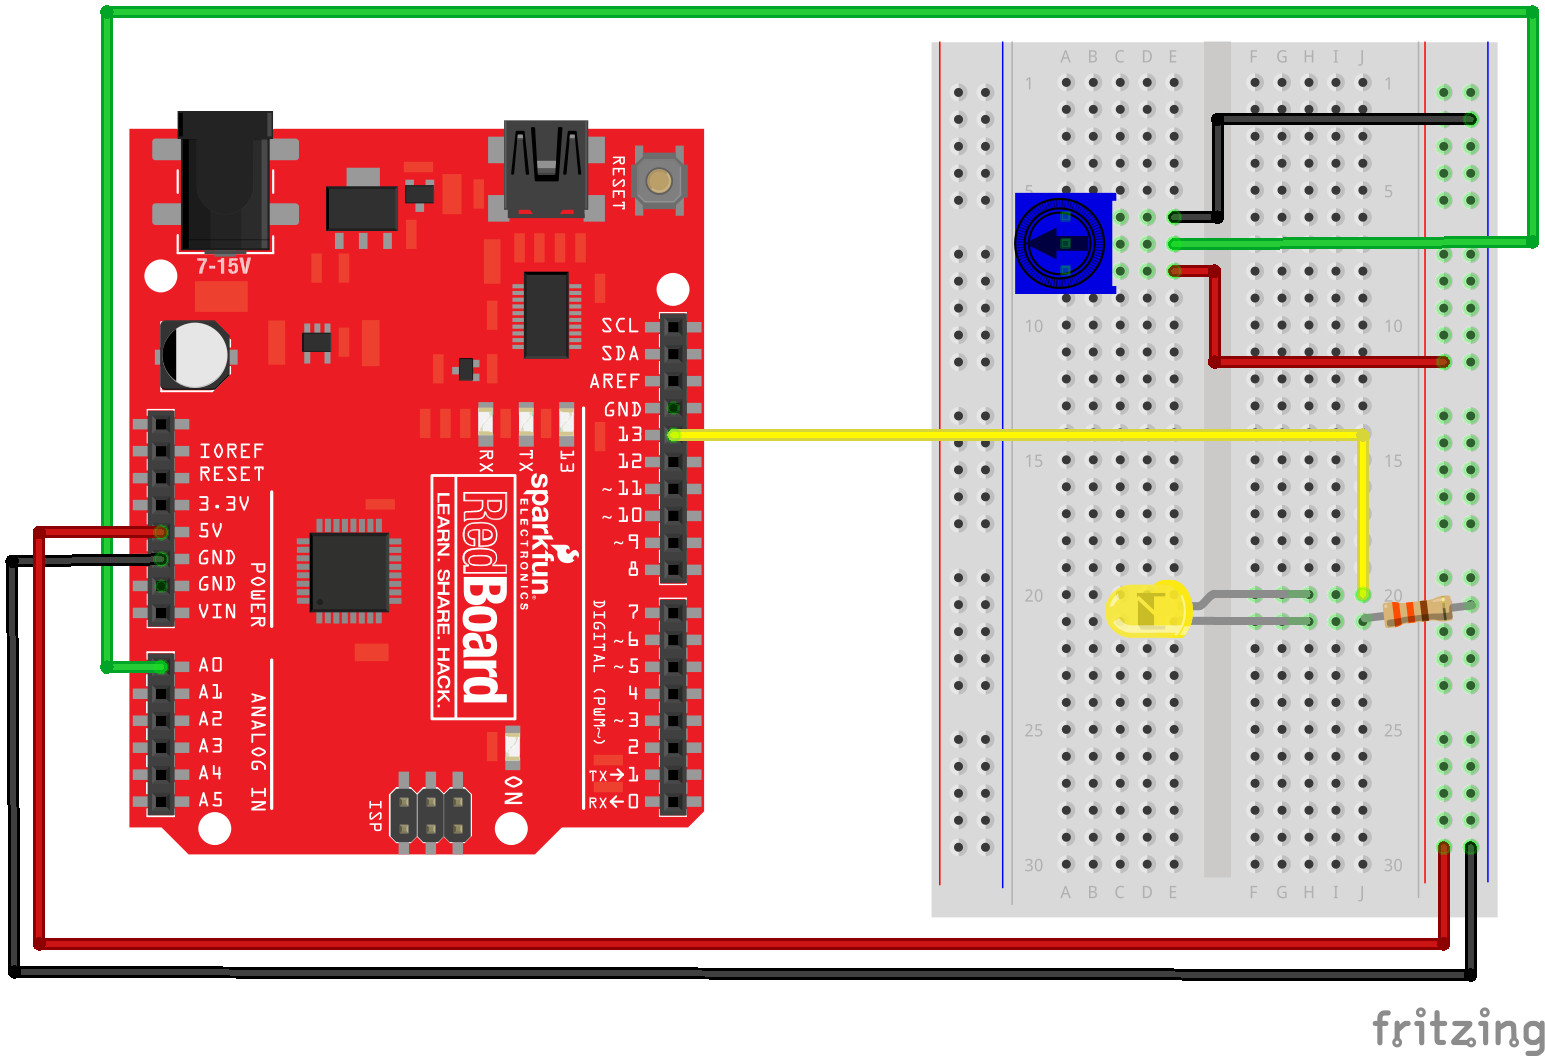
\includegraphics{images/redboard_pot_led_fritzing.png}
\caption{Arduino with potentiometer}
\end{figure}
    




    
        \subsection{Upload code to the
Arduino}\label{upload-code-to-the-arduino}
    




    
        Once the LED and potentiometer is hooked up the the Arduino, upload the
following code to the Arduino using the Arduino IDE. Note that Arduinos
don't use the Python programming language. The programming language used
by Arduinos is a varient of the C programming language.

The Arduino sketch (an Arduino program is called a sketch) below
accomplishes a couple things. First the Arduino reads the sensor value
and stores the sensor value to the variable \lstinline!sensorValue!.
Then the Arduino sends the sensor value over the serial line (as a byte
sting). Next, the sensor value is compared to 500. If the sensor value
is less than 500, the LED stays off. If the sensor value is greater than
500, the LED turn on. This process repeats in a loop.
    




    
        \begin{lstlisting}
// potentiometer_read.ino
// reads a potentiometer and sends value over serial
int sensorPin = A0;    // The potentiometer is connected to analog pin 0                  
int ledPin = 13;      // The LED is connected to digital pin 13
int sensorValue;     // an integer variable to store the potentiometer reading

void setup() // this function runs once when the sketch starts
{
  // make the LED pin (pin 13) an output pin
  pinMode(ledPin, OUTPUT);

  // initialize serial communication
  Serial.begin(9600);
}

void loop() // this function runs repeatedly after setup() finishes
{
  sensorValue = analogRead(sensorPin);  // read the voltage at pin A0   
  Serial.println(sensorValue);         // Output sensor value to Serial Monitor
  
  if (sensorValue < 500) {            // if sensor reading is less than 500,
    digitalWrite(ledPin, LOW); }     // Turn the LED off
  
  else {                               // if sensor reading is greater than 500
    digitalWrite(ledPin, HIGH); }     // Keep the LED on
  
  delay(100);             // Pause 100 milliseconds before next sensor reading
}
\end{lstlisting}
    




    
        \subsection{Connect the Arduino to the computer and Upload the
Sketch}\label{connect-the-arduino-to-the-computer-and-upload-the-sketch}
    




    
        Connect the Arduino to the computer with a USB cable. Upload the sketch
to the Arduino. In the Arduino IDE, click the {[}check mark{]} to verify
and the {[}arrow{]} to upload. If the sketch does not upload, check
which \lstinline!COM port! is selected in Tools --\textgreater{} Ports.

\begin{figure}
\centering

\includegraphics{images/Check_to_Verify.png}
\caption{Arduino IDE Check to Verify}
\end{figure}

\begin{figure}
\centering
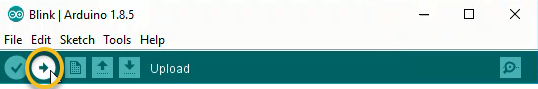
\includegraphics{images/Arrow_to_Upload.png}
\caption{Arduino IDE Arrow to Upload}
\end{figure}
    




    
        \subsection{Check the Sensor Signal}\label{check-the-sensor-signal}
    




    
        To verify the Arduino sketch is working correctly, the sensor signal can
be checked in three ways:

\begin{itemize}
\tightlist
\item
  The LED turns on and off as the potentiometer dial is turned
\item
  In the Arudino \textbf{Serial Monitor}, numbers change as the
  potentiometer dial is turned
\item
  In the Arduino \textbf{Seral Plotter}, the line moves as the
  potentiometer dial is turned
\end{itemize}
    




    
        \subsubsection{LED turns ON and OFF}\label{led-turns-on-and-off}

The LED should turn on and off as the potentiometer is turned. If the
LED does note turn on and off when the poteniometer is turned, make sure
the potentiometer is turned back and forth through it's full range of
rotation. Ensure the USB cable is plugged in to both the Arudino and the
computer.
    




    
        \subsubsection{Arudino Serial Monitor}\label{arudino-serial-monitor}

Access the Arduino \textbf{Serial Monitor} using Tools --\textgreater{}
Serial Monitor.

\begin{figure}
\centering
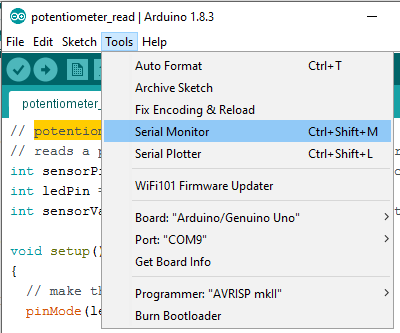
\includegraphics{images/Tools_SerialMonitor.png}
\caption{Select the Arudino Serial Monitor from the Tools Menus}
\end{figure}
    




    
        If the sketch is working correctly, a running list of numbers is shown
in the Arduino \textbf{Serial Monitor}. The output in the Serial Monitor
should be a running list of numbers between \lstinline!0! and
\lstinline!1024!. When the potentiometer is dialed back and forth, the
numbers streaming down the \textbf{Serial Monitor} should change. If
output can't be seen in the \textbf{Serial Monitor}, ensure {[}Auto
Scroll{]}, {[}Both NL \& CR{]} and {[}9600 baud{]} are selected. Also
make sure the \lstinline!Port! is set correctly in Tools
--\textgreater{} Port.

\begin{figure}
\centering
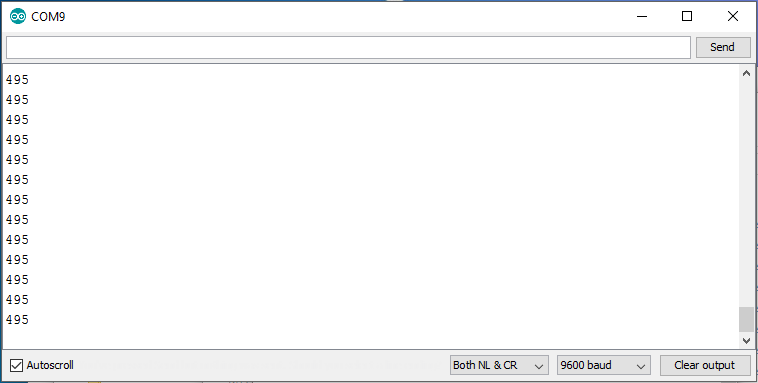
\includegraphics{images/serial_monitor_output.png}
\caption{Arduino Serial Monitor Ouput}
\end{figure}
    




    
        \subsubsection{Arduino Serial Plotter}\label{arduino-serial-plotter}

To access the Arduino Serial Plotter, use Tools --\textgreater{} Serial
Monitor. Note the Serial Monitor needs to be closed before the Serial
Plotter can be opened. If the sketch is working correctly, potentiometer
rotation produces a moving line on the Arduino Serial Plotter .

\begin{figure}
\centering
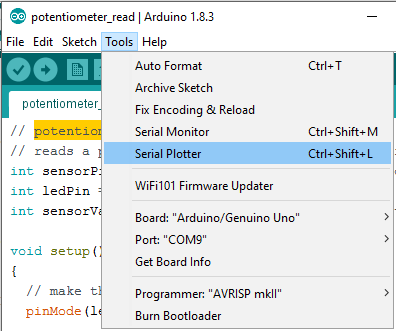
\includegraphics{images/Tools_SerialPlotter.png}
\caption{Arduino Serial Plotter Menu}
\end{figure}

The output of the Serial Plotter should be a running line graph. The
height of the line on the graph should change as the potentiometer is
dialed back and forth. If the Serial Plotter is blank, make sure {[}9600
baud{]} is selected in the lower right corner of the Serial Plotter.
Also make sure the \lstinline!Port! has been set correctly in Tools
--\textgreater{} Port.

\begin{figure}
\centering
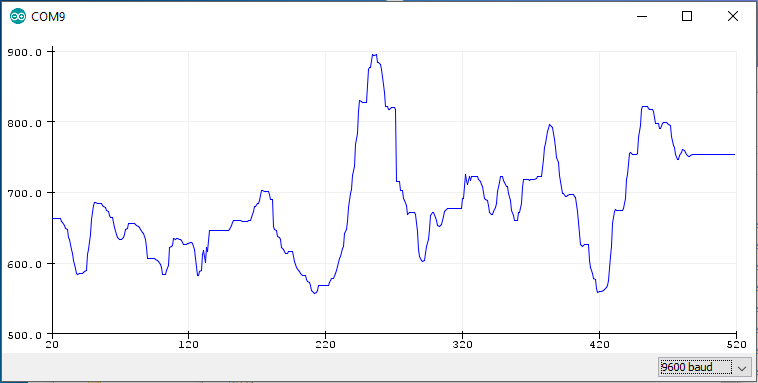
\includegraphics{images/serial_plotter_output.png}
\caption{Arudino Serial Plotter}
\end{figure}
    




    
        \subsection{Write a Pyton script to read the
sensor}\label{write-a-pyton-script-to-read-the-sensor}
    




    
        Once the hardware is connected and the Arduino sketch is working
properly, a Python script can be constructed to read the sensor value.

Communication between the Python script and the Arduino an be
accomplished using the \textbf{PySerial} package. Make sure
\textbf{PySerial} is installed before the script is run. At the top of
the Python script, import the \textbf{PySerial} module. Note that
although the package is called \textbf{PySerial}, use
\lstinline!import serial! to import the package.
    




    
        \begin{lstlisting}[language=Python]
import serial
import time
\end{lstlisting}
    




    
        Next, code a loop that will run for about 5 seconds while data is
collected from the sensor. If it seems like the loop is stuck, press
{[}Ctrl{]} + {[}c{]}.
    




    
        \begin{lstlisting}[language=Python]
data = [] # create an empty list to store the data
for i in range(50):
    with serial.Serial('COM4', 9800, timeout=1) as ser:
        line = ser.readline()   # read a '\n' terminated line
        string = line.decode()  # convert the byte string to a unicode string
        data.append(float(string)) # convert the unicode string to a float and add to the data list
        time.sleep(0.1) # wait 0.1 seconds before reading the next line
\end{lstlisting}
    




    
        After the data has been collected, it can be displayed with the
\lstinline!print()! function and a \lstinline!for! loop. The output
should look like the numbers in the Arduino \textbf{Serial Monitor}.
    




    
        \begin{lstlisting}[language=Python]
for line in data:
    print(line)
\end{lstlisting}
    




    
        The data can also be plotted with \textbf{matplotlib}. The plot should
look like the line plot in the Arduino \textbf{Serial Plotter}.
    




    
        \begin{lstlisting}[language=Python]
import matplotlib.pyplot as plt
# if using a jupyter notebook include, comment out if using a .py file
%matplotlib inline

plt.plot(data)
plt.show()
\end{lstlisting}
    




    
        \section{Controlling an LED with
Python}\label{controlling-an-led-with-python}
    




    
        In this section you will learn how to control an LED connected to an
external piece of hardware (an Arduino) using Python. To accomplish this
task the following hardware is required:

\begin{itemize}
\tightlist
\item
  A computer running Python
\item
  An Arduino
\item
  An LED
\item
  Wires, a resistor and a breadboard to connect the LED to the Arduino
\item
  A USB cable to connect the Arduino to the computer
\end{itemize}
    




    
        \subsection{Set up the LED}\label{set-up-the-led}
    




    
        Connect the LED to the Arduino using a resistor, wires and a breadboard.
Note the short leg of the resistor is connected to ground and the long
leg of the resistor is through a resistor to PIN 13. A resistor is
needed to prevent too much current from flowing through the LED. This
type of resistor is called a \emph{pull up resistor}.
    




    
        \begin{figure}
\centering
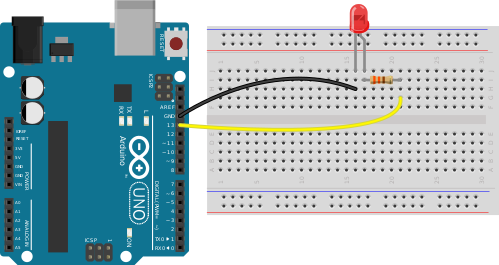
\includegraphics{images/arduino_LED.png}
\caption{Arduino with LED}
\end{figure}
    




    
        \subsection{Upload code to the
Arduino}\label{upload-code-to-the-arduino}
    




    
        Upload the following code to the Arduino using the Arduino IDE. This is
the example sketch called \lstinline!Physical Pixel!. The
\lstinline!Physical Pixel! sketch can be found in the Arduino IDE by
going to File --\textgreater{} Examples --\textgreater{}
04.Communication --\textgreater{} PhysicalPixel

\begin{figure}
\centering
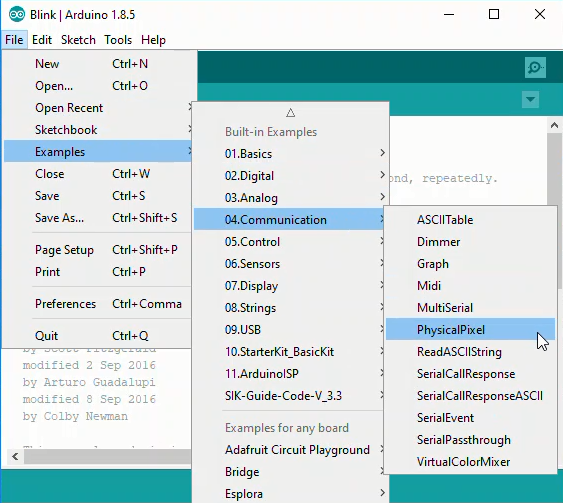
\includegraphics{images/file-examples-communication-physicalpixel.png}
\caption{Physical Pixel Example Sketch in the Arduino IDE}
\end{figure}

The code for the Physical Pixel Sketch is shown below. Note that
Arduinos don't use the Python programming language.
    




    
        \begin{lstlisting}
//  Arduino IDE: File --> Examples --> 04.Communication --> PhysicalPixel

const int ledPin = 13; // the pin that the LED is attached to
int incomingByte;      // a variable to read incoming serial data into

void setup() {
  // initialize serial communication:
  Serial.begin(9600);
  // initialize the LED pin as an output:
  pinMode(ledPin, OUTPUT);
}

void loop() {
  // see if there's incoming serial data:
  if (Serial.available() > 0) {
    // read the oldest byte in the serial buffer:
    incomingByte = Serial.read();
    // if it's a capital H (ASCII 72), turn on the LED:
    if (incomingByte == 'H') {
      digitalWrite(ledPin, HIGH);
    }
    // if it's an L (ASCII 76) turn off the LED:
    if (incomingByte == 'L') {
      digitalWrite(ledPin, LOW);
    }
  }
}
\end{lstlisting}
    




    
        \subsection{Connect the Arduino to the
Computer}\label{connect-the-arduino-to-the-computer}
    




    
        Connect the Arduino to the computer using a USB cable. Make sure the
\lstinline!Port! is selected properly in the Arduino IDE under Tools
--\textgreater{} Port.

In the Arduino IDE, click the {[}checkmark{]} to verify and the
{[}arrow{]} to upload. If the sketch does not upload, check which COM
port is selected in Tools --\textgreater{} Port.

\begin{figure}
\centering

\includegraphics{images/Check_to_Verify.png}
\caption{Arduino IDE Check to Verify}
\end{figure}

\begin{figure}
\centering
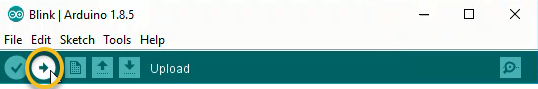
\includegraphics{images/Arrow_to_Upload.png}
\caption{Arduino IDE Arrow to Upload}
\end{figure}
    




    
        \subsection{Turn the LED on and off with the Arduino Serial
Monitor}\label{turn-the-led-on-and-off-with-the-arduino-serial-monitor}
    




    
        Bring up the Arduino Serial Monitor and type \lstinline!L! or
\lstinline!H! and click {[}Send{]} and observe the LED turn on and off.

\begin{figure}
\centering
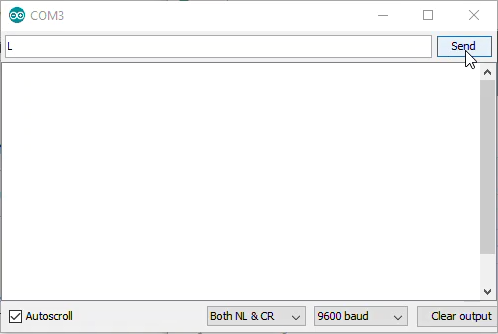
\includegraphics{images/serial_monitor_L.png}
\caption{Arduino Serial Monitor}
\end{figure}
    




    
        \subsection{Write a Pyton Script to turn the LED on and
off}\label{write-a-pyton-script-to-turn-the-led-on-and-off}
    




    
        After the LED turns on and off based on input at the Arduino Serial
Monitor, it is time to write a Python script to turn the LED on and off.
This can be accomplished using the \textbf{PySerial} package. Make sure
\textbf{PySerial} is installed before script is run.

At the top of the script, import the \textbf{PySerial} module. Note that
even though the package is called \textbf{PySerial} the line
\lstinline!import serial! is used. The \textbf{time} module is also
imported as the \lstinline!time.sleep()! function will be used in the
script.
    




    
        \begin{lstlisting}[language=Python]
import serial
import time
\end{lstlisting}
    




    
        In the next part of the Python script, create a loop that will blink the
LED on and off for about 5 seconds. Note the byte string
\lstinline!b'H'! need to be sent to the Arduino, not the unicode string
\lstinline!'H'!. The unicode string \lstinline!'H'! is pre-pended with
the letter \lstinline!b! in \lstinline!ser.writelines(b'H')!.
    




    
        \begin{lstlisting}[language=Python]
data = []
for i in range(10):
    with serial.Serial('COM4', 9800, timeout=1) as ser:
        ser.writelines(b'H')   # send a byte
        time.sleep(0.5)        # wait 0.5 seconds before reading the next line
        ser.writelines(b'L')   # send a byte
\end{lstlisting}
    




    
        \subsection{Write a Python script to allow a user to turn the LED on and
off}\label{write-a-python-script-to-allow-a-user-to-turn-the-led-on-and-off}
    




    
        Once the LED blinks on and off successfully using a Python script, it is
time to write a new Python script that will allow a user to turn the LED
on and off. At the top of the new Python script import the
\textbf{PySerial} and \textbf{time} modules.
    




    
        \begin{lstlisting}[language=Python]
import serial
import time
\end{lstlisting}
    




    
        Next, give the user instructions. If the user types \lstinline!H!, the
LED will turn on. If the user types \lstinline!L! the LED will turn off.
If the user types \lstinline!q!, the program will quit.
    




    
        \begin{lstlisting}[language=Python]
print('This is a program that allows a user to turn an LED on and off')
print('type H to turn the LED on')
print('type L to turn the LED off')
print('type q to quit')
\end{lstlisting}
    




    
        Finally, the script needs a while loop to ask the user for an
\lstinline!H! or \lstinline!L! character. Once the user enters the
letter, the letter needs to be converted to a byte string. Then the byte
string is sent over the serial line to the Arduino. A delay is added so
that the Arduino can process the previous command before dealing with
the next one.
    




    
        \begin{lstlisting}[language=Python]
user_input = input('H = on, L = off, q = quit' : )
while user_input != 'q':
    with serial.Serial('COM4', 9800, timeout=1) as ser:
        byte_command = encode(user_input)
        ser.writelines(byte_command)   # send a byte
        time.sleep(0.1) # wait 0.5 seconds before reading the next line
        user_input = input('H = on, L = off, q = quit' : )
print('q entered. Exiting the program')
\end{lstlisting}
    




    
        When the script is running, type \lstinline!H! and \lstinline!L! and
observe the LED blink on and off.
    




    
        \newpage
        \section{Summary}\label{summary}

    




    
        \subsection{Key Terms and Concepts}\label{key-terms-and-concepts}
    




    
        \begin{key_terms}
        External Hardware

Sensor

LED

Resistor

breadboard

Arduino

Serial Communication

USB

Unicode

Unicode String

UTF-8

Byte code

ASCII

ASCII Character
        \end{key_terms}

    




    
        \section{Review Questions}\label{review-questions}
    




    
        \begin{problems}
        \begin{enumerate}
\def\labelenumi{\arabic{enumi}.}
\item
\item
\item
\item
\item
\item
\item
\item
\item
\item
\end{enumerate}
        \end{problems}

    




    
        \chapter{MicroPython}\label{micropython}
    




    
        \section{Introduction}\label{introduction}
    




    
        By the end of this chapter you will be able to:

\begin{itemize}
\item
  Install MicroPython on a microcontroller
\item
  Run Python commands on a microcontroller using the MicroPython REPL
\item
  Save module files and run Python scripts on a microcontroller
\item
  Use MicroPython to read sensor data using a microcontroller
\item
  Use MicroPython to activate a relay using a microcontroller
\end{itemize}
        \newpage



    




    
        \section{What is MicroPython?}\label{what-is-micropython}
    




    
        \subsection{What is MicroPython?}\label{what-is-micropython}
    




    
        \href{http://micropython.org/}{MicroPython} is a port, or version of
Python designed to run on small, inexpensive, low-power
microcontrollers. Examples of microcontrollers that Micropython can run
on include the \href{https://store.micropython.org/}{pyboard}, the
\href{https://pycom.io/development-boards}{WiPy} and ESP8266 boards like
the
\href{https://learn.adafruit.com/adafruit-feather-huzzah-esp8266}{Adafruit
Feather Huzzah}. Normally, Python is run on a desktop or laptop computer
(also on big servers at server farms). Compared to a desktop or laptop,
microcontrollers are much smaller, cheaper and less powerful. A
``regular'' version of Python can't run on small, cheap microcontrollers
because Python is too resouce intensive. Regular Python takes up too
much hard disk space, runs on too much RAM and requires a more powerful
processor than microcontrollers have.

It is pretty amazing that a version of Python (MicroPython) runs on
these small, cheap microcontrollers like the ESP8266. To get MicroPython
to run at all on these small boards, MicroPython only contains a subset
of all the standard library modules included with ``regular'' Python.
Some of the libraries that are included with MicroPython don't have the
full set of functions and classes that come with the full version of
Python. This allows MicroPython to be compact (around 600 kB for the
ESP8266 port) and only use a small amount of RAM (down to 16k according
to the \href{https://micropython.org/}{Micropython main page})

You can try using MicroPython online with this neat
\href{https://micropython.org/unicorn/}{MicroPython online emulator}.
The emulator allows you to run commands at a MicroPython Prompt and see
the result on a virtual pyboard.
    




    
        \subsection{What is Micropython used
for?}\label{what-is-micropython-used-for}
    




    
        MicroPython is installed on small, cheap microcontrollers like the
\href{https://learn.adafruit.com/adafruit-feather-huzzah-esp8266}{ESP8266}.
Anything these small microcontrollers can do, MicroPython can do. This
includes using the microcontroller as a remote sensor to measure things
like temperature, humidity and light level. MicroPython can also be used
to blink LED's, control arrays of LED's, or run small displays.
MicroPython can control servo motors, stepper motors and solenoids.
Civil Engineers could use MicroPython to monitor water levels.
Michanical Engineers could use MicroPython to drive robots. Electrical
Engineers could use microPython to measure voltage levels in embedded
systems. In the later posts in this series, we will use MicroPython,
running on a small cheap ESP8266 board, to create a remote
Internet-connected weather station. The last posts in the series will
use MicroPython, running on a \textbf{really cheap} (around \$2) ESP-01
module to turn on and off an LED from any computer connected to the
Internet anywhere in the world.
    




    
        \subsection{Why should problem solvers learn
MircoPython?}\label{why-should-problem-solvers-learn-mircopython}
    




    
        Using Python to solve engineering problems such as calculations,
statistics, modeling and visualization is really useful for
undergraduate Engineers. But Python on it's own is fairly limited in
controlling devices outside the computer it's running on. You don't want
to leave a laptop in a remote estuary to measure water temperature, but
you could leave a little microcontroller and low-cost temperature
sensor. A small robot can't carry around a heavy laptop, but a small,
light, low-power board could run a simple robot. You don't want to use a
laptop for every small electrical measurement or embedded system
control, but a \$2 WiFi module would work.

In addition, learning how to use MicroPython on small, cheap
microcontrller can help undergraduates Engineers understand how
programming works. It is a different kind of feedback and excitement
seeing a motor whirl around compared to seeing a picture of a motor with
the speed displayed as text. There is a different kind of wonder seeing
an array of LED's light up compared to a 2-D plot on a computer screen.
Plus MicroPython is just fun! It's as easy to program MicroPython as it
is to program regular Python. The little projects you can do with
MicroPython running on a small, low-cost board are almost unlimited. We
could send MicroPython to space in a micro-satellite, or bury
MicroPython underground in a small boring machine, or launch MicorPython
into the sky on a weather balloon.
    




    
        \section{Installing MicroPython}\label{installing-micropython}
    




    
        MicroPython is a port of the Python programming language that runs on
small, inexpensive microcontrollers. In this section, you will learn how
to install MicroPython on an Adafruit Feather Huzzah ESP8266
microcontroller using Python and a package called \textbf{esptool}. In
subsequent sections, you will learn how to blink an LED and read a
sensor using MicroPython.
    




    
        To install MicroPython on an ESP8266-based microcontroller, like the
Adafruit Feather Huzzah ESP8266, we need the following hardware:

\begin{longtable}[]{@{}ll@{}}
\toprule
Hardware & Purpose\tabularnewline
\midrule
\endhead
Windows 10 & install Micropython on the microcontroller\tabularnewline
Adafruit Feather Huzzah ESP8266 & microcontroller running
MicroPython\tabularnewline
microUSB cable & connect microcontroller to computer\tabularnewline
\bottomrule
\end{longtable}

To install MicroPython we will use the following software and tools:

\begin{longtable}[]{@{}ll@{}}
\toprule
Software & Purpose\tabularnewline
\midrule
\endhead
Windows 10 & download MicroPython\tabularnewline
Anaconda distribution of Python & run \textbf{esptool} that installs
MicroPython\tabularnewline
Anaconda Prompt & Install the \textbf{esptool} package using
\textbf{pip}\tabularnewline
\textbf{esptool} & A \textbf{pip} installable package used to install
MicroPython\tabularnewline
firmware \textbf{\emph{.bin}} file & Version of MicroPython run on the
microcontroller\tabularnewline
\bottomrule
\end{longtable}
    




    
        \subsection{Summary of Steps:}\label{summary-of-steps}
    




    
        \begin{enumerate}
\def\labelenumi{\arabic{enumi}.}
\tightlist
\item
  Install the \href{https://www.anaconda.com/download/}{Anaconda
  distribution} of Python
\item
  Create a new conda environment and \lstinline!pip install esptool!
\item
  Download the \href{http://micropython.org/download\#esp8266}{latest
  MicroPython .bin firmware file}
\item
  Install the
  \href{https://www.silabs.com/products/development-tools/software/usb-to-uart-bridge-vcp-drivers}{SiLabs
  driver} for the Adafruit Feather Huzzah ESP8266
\item
  Connect the Adafruit Feather Huzzah ESP8266 board to the laptop using
  a microUSB cable
\item
  Determine which serial port the Feather Huzzah is connected to
\item
  Run the esptool to upload the .bin firmware file to the Feather Huzzah
\item
  Download and install \href{https://www.putty.org/}{Putty}, a serial
  monitor
\item
  Use Putty to connect to the Feather Huzzah and run commands in the
  MicroPython REPL
\end{enumerate}
    




    
        \subsection{Install the Anaconda distribution of
Python}\label{install-the-anaconda-distribution-of-python}
    




    
        If you don't have Anaconda installed already, go to
\href{https://www.anaconda.com/download/}{Anaconda.com/download} and
install the latest version.
    




    
        \subsection{\texorpdfstring{Create a new conda environment and install
\textbf{esptool}}{Create a new conda environment and install esptool}}\label{create-a-new-conda-environment-and-install-esptool}
    




    
        It's best practice when using Python to work in virtual environments.
We'll create a new virtual environment with conda to use with our
MicroPython projects. Open the Anaconda prompt and create a new virtual
environment named \lstinline!micropython!. Activate the environment with
the \lstinline!conda activate! command. After activating the virtual
environment you should see \lstinline!(micropython)! before the Anaconda
Prompt. Once inside the virtual environment, use \lstinline!pip! to
install \lstinline!esptool!. The \lstinline!esptool! will be used to
upload the MicroPython .bin firmware file onto the Adafruit Feather
Huzzah board. Confirm that \lstinline!esptool! is installed in the
\lstinline!(micropython)! virtual environment with
\lstinline!conda list!. I also created a new directory in the
\textbf{Documents} folder called \textbf{micropython} to store all the
project files.

\begin{lstlisting}
> conda create -n micropython python=3.6
> conda activate micropython
(micropython) > pip install esptool
(micropython) > conda list
(micropython) > cd Documents
(micropython) > mkdir micropthon
(micropython) > cd micropython
\end{lstlisting}
    




    
        \subsection{Download the latest MicroPython firmware .bin
file}\label{download-the-latest-micropython-firmware-.bin-file}
    




    
        Go to github.com and
\href{https://micropython.org/download\#esp8266}{download the latest
.bin firmware} file at micropython.org/download\#esp8266. Move the
\textbf{\emph{.bin}} firmware file to a new \textbf{micropython}
directory. The \textbf{\emph{.bin}} firmware file is the version of
Micropython that will run on the Adafruit Feather Huzzah ESP8266.
Straight from Adafruit, the Feather Huzzah microcontroller does not have
Micropyton installed, so we need to install Micropython ourselves. After
installing the Micropython .bin firmware file onto the board, we will be
able to bring up the Micropython REPL prompt, type commands into the
Micropython REPL and run Micropython \textbf{\emph{.py}} scripts on the
board.

\begin{figure}
\centering
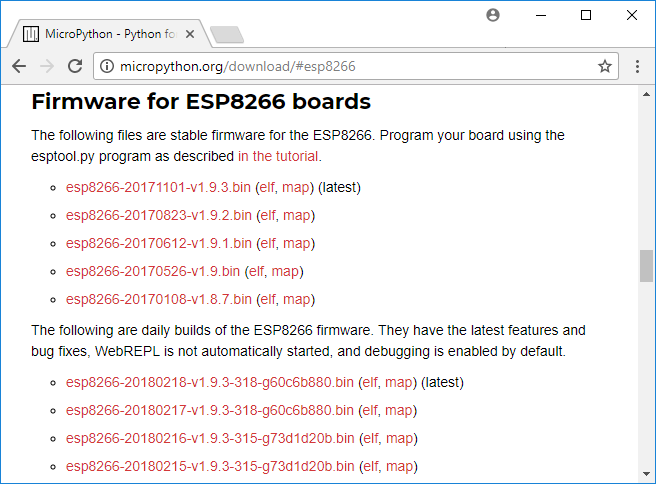
\includegraphics{images/firmware_download_page.PNG}
\caption{MicroPython Firmware}
\end{figure}
    




    
        \subsection{Install the SiLabs driver for the Adafruit Feather Huzzah
ESP8266}\label{install-the-silabs-driver-for-the-adafruit-feather-huzzah-esp8266}
    




    
        Before we can connect the Adafruit Feather Huzzah to the computer, we
need a specific driver installed. For my Windows 10 laptop to see the
Adafruit Feather Huzzah board, the
\href{https://www.silabs.com/products/development-tools/software/usb-to-uart-bridge-vcp-drivers}{CP210x
USB to UART Bridge VCP driver} needs to be downloaded from SiLabs and
installed. This is quick and easy, but does require admin privileges.

\begin{figure}
\centering
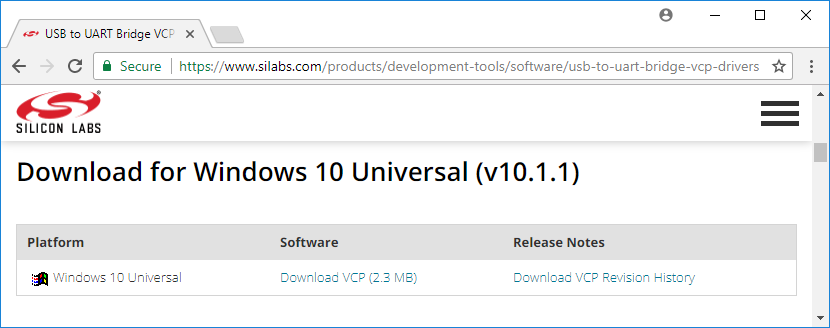
\includegraphics{images/download_silabs_driver.PNG}
\caption{SiLabs Driver Download Page}
\end{figure}
    




    
        \subsection{Connect the Adafruit Feather Huzzah ESP8266 board to the
laptop}\label{connect-the-adafruit-feather-huzzah-esp8266-board-to-the-laptop}
    




    
        Use a microUSB cable (the same kind of cable that charges many mobile
phones) to connect the Feather Huzzah to the computer. Make sure that
the microUSB cable is a full USB \textbf{data cable} and not just a
simple power cable. If you have trouble getting the Feather Huzzah to
work, one reason might be the micoUSB cable is only a charging cable and
can not transfer data.
    




    
        \subsection{Determine which serial port the Feather Huzzah is connected
to}\label{determine-which-serial-port-the-feather-huzzah-is-connected-to}
    




    
        Use Windows Device Manager to determine which serial port the Feather
Huzzah board is connected to. The serial port is one of the parameters
that needs to be defined when the .bin firmware file is upload on the
board. Look for something like \textbf{Silicon Labs CP210x USB to UART
Bridge (COM4)} in the \textbf{Ports (COM \& LPT)} menu. The USB to UART
bridge is actually the Feather Huzzah board. CP210x refers to the chip
that handles serial communication on the Feather Huzzah, not the ESP8266
chip itself. Make note of the number after \textbf{(COM )}. It often
comes up as \textbf{(COM4)} but it may be different on your machine.

\begin{figure}
\centering
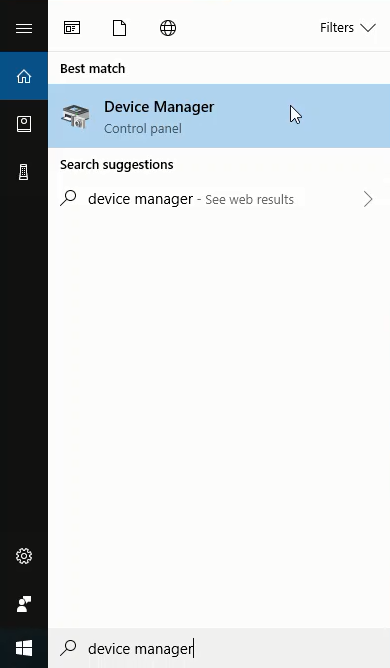
\includegraphics{images/find_device_manager.png}
\caption{Find Windows 10 Device Manager}
\end{figure}

\begin{figure}
\centering
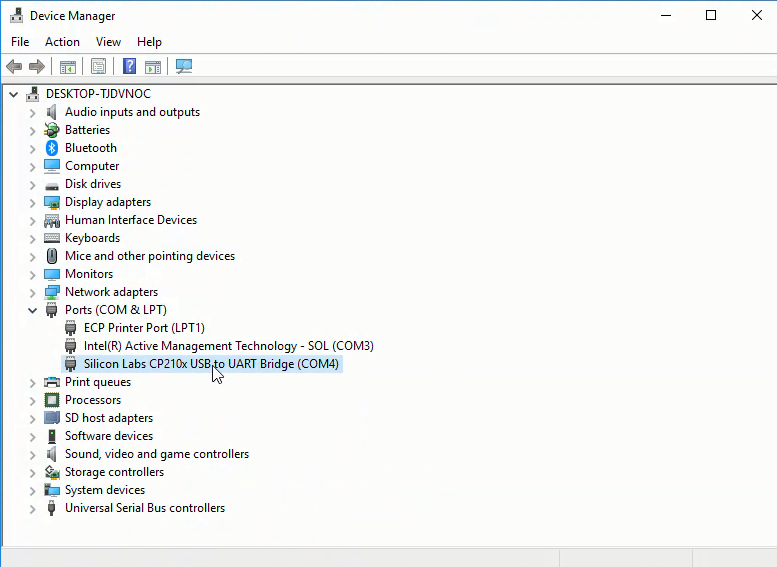
\includegraphics{images/device_manager_menu.png}
\caption{Windows 10 Device Manager Menu}
\end{figure}
    




    
        \subsection{Run esptool to upload the .bin file to the Feather
Huzzah}\label{run-esptool-to-upload-the-.bin-file-to-the-feather-huzzah}
    




    
        Open the Anaconda Prompt and \lstinline!cd! into the
\textbf{micropython} directory with the .bin file. You can use the
\lstinline!dir! command to see the directory contents. Make sure the
.bin firmware file is in the directory. It will be called something like
\lstinline!esp8266-20171101-v1.9.3.bin!. Activate the micropython
environment with \lstinline!conda activate micropython!. Run
\lstinline!esptool --help! to ensure esptool is installed properly. Note
there is no \textbf{.py} extension after \lstinline!esptool!. On my
Windows laptop, the command \lstinline!esptool! worked, but the command
\lstinline!esptool.py! did not (this is different than the commands
shown on the
\href{https://docs.micropython.org/en/latest/esp8266/esp8266/tutorial/intro.html\#deploying-the-firmware}{MicroPython
docs}). If you try to run esptool and you are not in the
\lstinline!(micropython)! virtual environment, you will get an error.

\begin{lstlisting}
> cd Documents
> cd micropython
> pwd
Documents/micropython
> dir
> conda activate micropython
(micropython) > esptool --help
\end{lstlisting}

\begin{figure}
\centering
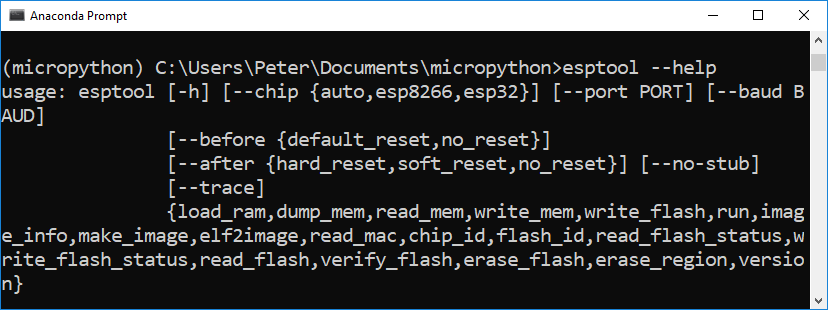
\includegraphics{images/esptool_help.PNG}
\caption{esptool help}
\end{figure}

Before we write the .bin firmware file to the board, we should first
erase the flash memory on the Feather Huzzah using the
\lstinline!esptool erase_flash! command. Make sure to specify the
\lstinline!--port!. This is the \lstinline!COM! port you found in the
Windows Device Manager. In my case the port was \lstinline!COM4!.

\begin{lstlisting}
(micropython) esptool --port COM4 erase_flash
\end{lstlisting}

\begin{figure}
\centering
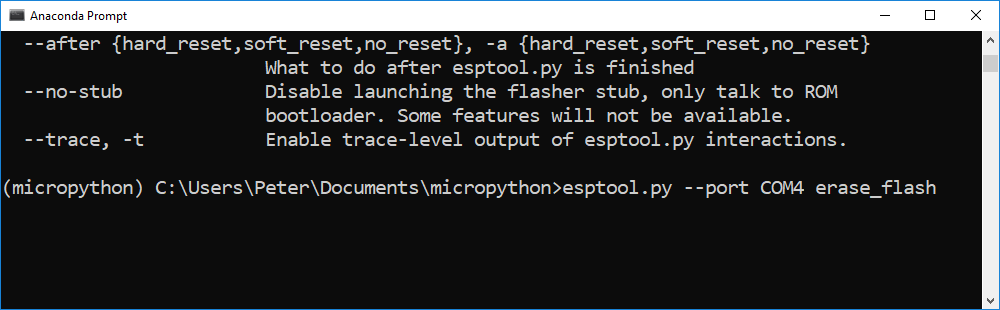
\includegraphics{images/esptool_erase_flash.PNG}
\caption{esptool erase flash}
\end{figure}

Now it's time to write the .bin firmware file to the flash memory on the
board using the \lstinline!esptool write_flash! command. Make sure to
use the exact .bin firmware file name you see sitting in the
\textbf{micropython} directory. The port has to be set as the port you
found in the Windows Device Manager. \lstinline!---baud! is the baud
rate, or upload speed. I found that \lstinline!--baud 460800! worked,
but you could also specify \lstinline!--baud 115200! which is slower.
The upload time was a matter of seconds with either baud rate. The
\lstinline!0! after \lstinline!--flash_size=dectect! means we want the
firmware to be written at the start of the flash memory (the 0th
position) on the board. Again, make sure the .bin firmware file name is
correct. It is easy to mistype. Another issue I ran into was that I
tried to use the command \lstinline!esptool.py! instead of
\lstinline!esptool! as shown on the
\href{https://docs.micropython.org/en/latest/esp8266/esp8266/tutorial/intro.html\#deploying-the-firmware}{MicroPython
docs}. The documentation for
\href{https://docs.micropython.org/en/latest/esp8266/esp8266/tutorial/intro.html\#deploying-the-firmware}{MicroPython
on the ESP8266} specifies the command \lstinline!esptool.py! (including
the \textbf{\emph{.py}} file extension). This did work on my Windows 10
machine. Omitting the \textbf{\emph{.py}} file extension, and running
\lstinline!esptool! worked instead.

\begin{lstlisting}
(micropython) > esptool --port COM4 --baud 460800 write_flash --flash_size=detect 0 esp8266-20171101-v1.9.3.bin
\end{lstlisting}

\begin{figure}
\centering
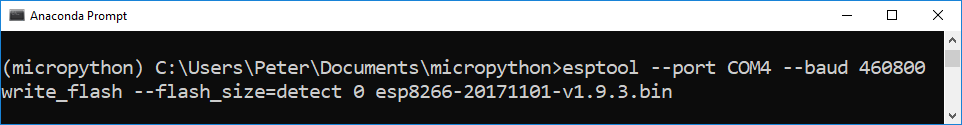
\includegraphics{images/esptool_write_flash.PNG}
\caption{Use esptool to upload MicroPython firmware}
\end{figure}
    




    
        \subsection{Download and install PuTTY, a serial
monitor}\label{download-and-install-putty-a-serial-monitor}
    




    
        Now that MicroPython is installed on the board, we need to talk to our
board over a serial connection. Windows 10 doesn't have a built-in
serial monitor (like screen on OSX and Linux). So we need to download
and install \textbf{PuTTY}. PuTTY is a lightweight SSH and serial client
for Windows. PuTTY will allow us to communicate with the Adafruit
Feather Huzzah board. \href{https://www.putty.org/}{PuTTY can be
downloaded here}. PUTTY is pretty small and the download and install
should be pretty quick.

\begin{figure}
\centering
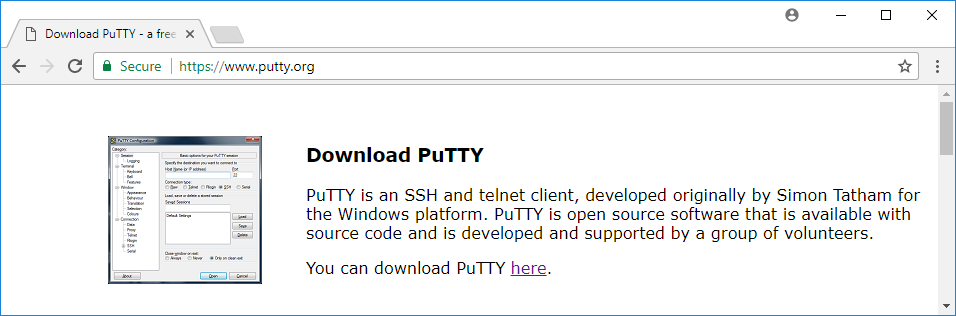
\includegraphics{images/download_putty.PNG}
\caption{PuTTY Downloads Page}
\end{figure}
    




    
        \subsection{Use PuTTY to connect to the Feather
Huzzah}\label{use-putty-to-connect-to-the-feather-huzzah}
    




    
        Ensure the Feather board is connected to the computer with a USB cable
and ensure you can see the board in the Windows Device Manager. Then use
Putty to connect to the board over serial. Make sure you specify the
correct serial port in the \textbf{Serial line} box and \textbf{115200}
baud in the Speed box. \textbf{Micropython is set to run at 115200
baud}, other baud rates will lead to junk characters in the serial
monitor. I had trouble finding the serial connection option in Putty.
When I opened Putty, the default was an SSH connection. We can't connect
to the Feather Huzzah over SSH. You need to select the \textbf{Serial}
radio button below the header \textbf{Connection type:} near the top of
the Putty window.

\begin{figure}
\centering
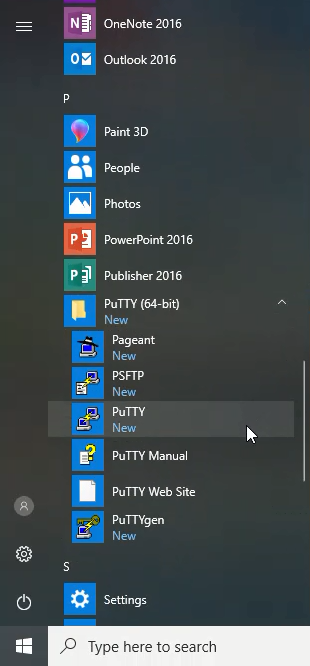
\includegraphics{images/putty_in_start_menu.png}
\caption{PuTTY in Windows 10 Start Menu}
\end{figure}

\begin{figure}
\centering
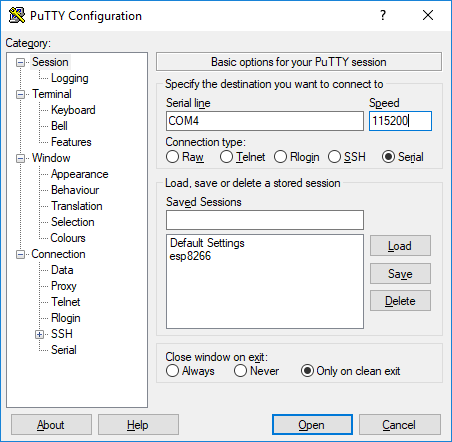
\includegraphics{images/putty_config.PNG}
\caption{PuTTY Configuration}
\end{figure}

If you see \lstinline!>>>! the MicroPython REPL (the MicroPython prompt)
is running and the Adafruit Feather Huzzah ESP8266 is working! This
version of Python isn't running on your computer, it's MicroPython
running on the little microcontroller! Sometimes I had to type
{[}Enter{]} or Ctrl-D to get the \lstinline!>>>! REPL prompt to show up.
A few times I needed to close Putty, unplug then replug the board and
try Putty again. The Feather Huzzah also has a tiny little black RESET
button that can be pressed to restart the board.

\begin{figure}
\centering
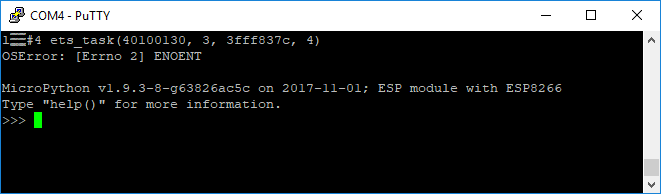
\includegraphics{images/REPL_prompt.PNG}
\caption{The MicroPython REPL Prompt}
\end{figure}

At the \lstinline!>>>! MicroPython REPL prompt try the following
commands:

\begin{lstlisting}
>>> print('MicroPython for Engineers!')
MicroPython for Engineers

>>> import sys
>>> sys.platform
'esp8266'
\end{lstlisting}

\begin{figure}
\centering
\includegraphics{images/sys_dot_platform.PNG}
\caption{result of commands typed in the MicroPython REPL}
\end{figure}
    




    
        \section{MicroPython REPL}\label{micropython-repl}
    




    
        The last section detailed the installation of MicroPython on an Adafruit
Feather Huzzah ESP8266 microcontroller using Python and a package called
\textbf{esptool}. In this section, you will learn how to write commands
to the MicroPython REPL (the Micropython prompt) to turn an LED on and
off.

Before you can use the MicroPython REPL (the MicroPython prompt) running
on the Adafruit Feather Huzzah ESP8266, MicroPython needs to be
installed on the board and PuTTY needs to be installed the Windows 10
computer to communicate with the board over serial. The previous section
detailed how to install MicroPython on an ESP8266 microcontroller and
how to install \href{https://www.putty.org/}{PuTTY} on a Windows 10
machine.
    




    
        \subsection{Summary of Steps}\label{summary-of-steps}
    




    
        \begin{enumerate}
\def\labelenumi{\arabic{enumi}.}
\tightlist
\item
  Connect the Adafruit Feather Huzzah ESP8266 using a USB cable
\item
  Determine which COM port the board is connected to using the Windows
  Device Manager
\item
  Open PuTTY and connect to the board at 115200 baud
\item
  Run commands at the prompt to turn the built-in LED on the Adafruit
  Feather Huzzah ESP8266 on and off
\end{enumerate}
    




    
        \subsection{Connect the Adafruit Feather Huzzah ESP8266 board to the
laptop}\label{connect-the-adafruit-feather-huzzah-esp8266-board-to-the-laptop}
    




    
        Use a microUSB cable to connect the microcontroller to the computer.
Make sure that the microUSB cable is a full USB data cable and not just
a simple power cable. Cables that are just used to charge phones may
only be power cables and may not be capable of transmitting data.
    




    
        \subsection{Determine which serial port the Feather Huzzah is connected
to}\label{determine-which-serial-port-the-feather-huzzah-is-connected-to}
    




    
        Use Windows Device Manager to determine which serial port the Feather
Huzzah is connected to. O Windows 10, the microcontroller usually comes
up as \lstinline!COM4!. You can find the serial port by looking in the
Ports (COM \& LPT) category of the Windows Device Manager. Look for
something like \textbf{Silicon Labs CP210x USB to UART Bridge (COM4)} in
the \textbf{Ports (COM \& LPT)} menu. It is the \textbf{COM\#} that you
are looking for.

\begin{figure}
\centering
\includegraphics{images/find_device_manager.png}
\caption{Find the Windows 10 Device Manager}
\end{figure}

\begin{figure}
\centering
\includegraphics{images/device_manager_menu.png}
\caption{Device Manager Menu on Windows 10}
\end{figure}
    




    
        \subsection{Use Putty to connect to the Feather
Huzzah}\label{use-putty-to-connect-to-the-feather-huzzah}
    




    
        Ensure the Feather Huzzah board is connected with a USB cable, then
connect to it with PuTTY using the proper serial port (COM\#) and 115200
baud. Remember to use the \textbf{Serial} radio button under
\textbf{Connection Type:} to select serial communication or you will be
trying to communicate with the Feather Huzzah over SSH which won't work.

\begin{figure}
\centering
\includegraphics{images/putty_in_start_menu.png}
\caption{PuTTY in Windows 10 start menu}
\end{figure}

\begin{figure}
\centering
\includegraphics{images/putty_config.PNG}
\caption{PuTTY configuration}
\end{figure}

This should bring up the MicroPython REPL prompt \lstinline!>>>!. If you
can't see the \lstinline!>>>! prompt, try typing {[}Enter{]}, Ctrl-D,
pushing the RESET button on the Feather Huzzah or unplugging then
replugging the USB cable.

\begin{figure}
\centering
\includegraphics{images/REPL_prompt.PNG}
\caption{MicroPython REPL prompt}
\end{figure}
    




    
        \subsection{Run commands at the prompt to turn the built-in LED on the
Adafruit Feather Huzzah ESP8266 on and
off}\label{run-commands-at-the-prompt-to-turn-the-built-in-led-on-the-adafruit-feather-huzzah-esp8266-on-and-off}
    




    
        At the MicroPython REPL (the MicroPython command prompt \lstinline!>>>!)
try the following commands:

\begin{lstlisting}
>>> print('MicroPython for Engineers!')
MicroPython for Engineers
\end{lstlisting}

If we import the \lstinline!sys! module, we can see the MicroPython
implementation and platform.

\begin{lstlisting}
>>> import sys
>>> sys.implementation
(name='micropython', version=(1, 9, 3))
>>> sys.platform
'esp8266'
\end{lstlisting}

\begin{figure}
\centering
\includegraphics{images/sys_dot_implementation_and_platform.PNG}
\caption{Results of running sys commands at the MicroPython REPL prompt}
\end{figure}

If you see similar output, that means MicroPython is working on the
Feather Huzzah. We can also view the flash memory size of our Feather
Huzzah and the size of the MicroPython firmware we installed. Try this
at the MicroPython prompt:

\begin{lstlisting}
>>> import port_diag
\end{lstlisting}

\begin{figure}
\centering
\includegraphics{images/import_port_diag.PNG}
\caption{Results of running import port\_diag at the MicroPython REPL
prompt}
\end{figure}

We can see the flash memory size is 4 MB. Below the label
\lstinline!Firmware checksum:! we can see a line for
\lstinline!size: 600872!. This means the size of our Micropythpon
installation is about 600 KB or 0.6 MB. Just over half a megabyte and we
are running a working version of Python!

Now let's turn the Feather Huzzah's built-in LED on and off. The Feather
Huzzah has a built-in red LED connected to Pin 0. We can access this LED
with MicroPython's \lstinline!machine! module.

First, we use the \lstinline!machine! module to create a \lstinline!Pin!
object. The first argument when we instantiate the \lstinline!Pin!
object is the pin number on the board (in this case \lstinline!0!). Pin
0 on the Feather Huzzah is connected to the built-in red LED. The second
argument is the pin type. We want Pin 0 to act as an output pin
(\lstinline!machine.Pin.OUT!). We are going to assign our
\lstinline!pin! the attribute \lstinline!.on()! or \lstinline!.off()!.
This will cause the Feather board to output a positive voltage or no
voltage to Pin 0 to turn the built-in red LED on and off. You can also
connect Pin 0 to an external LED through a resistor then to ground and
have this external LED turn on and off.

\begin{lstlisting}
>>> import machine
>>> pin = machine.Pin(0, machine.Pin.OUT)
\end{lstlisting}

Note that Pin 0 on the Adafruit Feather Huzzah is kind of wired
``backwards''. We call \lstinline!pin.off()! and the built-in LED turns
\textbf{on} and call \lstinline!pin.on()! and the built-in LED turns
\textbf{off}.

\begin{lstlisting}
>>> pin.on()
>>> pin.off()
>>> pin.on()
>>> pin.off()
\end{lstlisting}

Now let's see if we can make the LED blink. We'll do this with a simple
\lstinline!for! loop. At the MicroPython REPL, initiating a loop will
automatically indent the next line, so a tab is not needed before the
\lstinline!pin.on()! statement. To run the loop, type backspace on an
empty line (to backspace from an indented line) and hit {[}Enter{]}.

\begin{lstlisting}
>>> import time
>>> for i in range(10):
...     pin.on()
...     time.sleep(1)
...     pin.off()
...     time.sleep(1)
...
\end{lstlisting}

This will blink the LED on and off for a total of 20 seconds.
    




    
        \section{Blinking a LED}\label{blinking-a-led}
    




    
        In this section, you will learn how to blink the built-in LED on to an
Adafruit Feather Huzzah ESP8266 microcontroller using the MicroPython
REPL.

Before the LED on the Adafruit Feather Huzzah ESP8266 can be blinked,
MicroPython needs to be installed on the Feather Huzzah board and PuTTY
needs to be installed (if using Windows 10) to facilitate communication
between the Feather Huzzah board and the computer. Alternatively, the
MacOS or Linux terminal and \textbf{screen} can be used for serial
communication.
    




    
        The Feather Huzzah as a built-in red LED mounted on the board close to
the USB cable input. MicroPython can be used to blink this LED on and
off.
    




    
        \subsection{Connect the Adafruit Feather Huzzah to the computer with a
USB cable and bring up the MicroPython REPL using
PuTTY.}\label{connect-the-adafruit-feather-huzzah-to-the-computer-with-a-usb-cable-and-bring-up-the-micropython-repl-using-putty.}
    




    
        Connect the Adafruit Feather Huzzah ESP8266 to the computer with a
microUSB cable. Ensure this is a USB data cable, not just a charging
cable. Open Putty and connect to the Feather Huzzah using the proper
serial port (COM\#) and 115200 baud. (Remember to use the
\textbf{Serial} radio button under \textbf{Connection Type:})

\begin{figure}
\centering
\includegraphics{images/putty_in_start_menu.png}
\caption{PuTTY in the Windows 10 Start Menu}
\end{figure}

\begin{figure}
\centering
\includegraphics{images/putty_config.PNG}
\caption{PuTTY Configuration}
\end{figure}

This will bring up the MicroPython REPL prompt \lstinline!>>>!. If you
can't see the \lstinline!>>>! prompt, try typing {[}Enter{]} or Ctrl-D
or push the RESET button on the Feather Huzzah. If none of these methods
work, try closing Putty and unplugging then replugging in the USB cable.
    




    
        \subsection{Run code at the MicroPython REPL to turn the LED on and
off}\label{run-code-at-the-micropython-repl-to-turn-the-led-on-and-off}
    




    
        In the PuTTY serial window, test to see if the MicroPython REPL is
functioning with a basic \emph{Hello World} program.

\begin{lstlisting}
>>> print("Hello World")
Hello World
\end{lstlisting}

Next, we will blink the Feather Huzzah's built-in LED. The Feather
Huzzah has a built-in LED connected to Pin 0. If we control the current
going to Pin 0, we control the built-in LED. To control a Pin using
MicroPython, first the \textbf{machine} module needs to be imported.
Next a \lstinline!Pin! object needs to be created. The integer passed
into \lstinline!machine.Pin()! determines the pin number assigned to the
\lstinline!Pin! object.

\begin{lstlisting}
>>> import machine
>>> pin = machine.Pin(0)
\end{lstlisting}

The value (on or off) of Pin 0 can be returned using

\begin{lstlisting}
>>> pin.value
1
\end{lstlisting}

To assign a value to Pin 0, the \lstinline!Pin! object must be created
as an \emph{output} pin. An output pin is a pin where a program or user
determines the pin output. An input pin is a pin set up to read input,
like the input from a sensor. In this case we want to assign Pin 0 as an
output pin.

\begin{lstlisting}
>>> pin = machine.Pin(0, machine.Pin.OUT)

# turn the LED on
>>> pin.value(0)

# turn the LED off
>>> pin.value(1)
\end{lstlisting}
    




    
        \subsection{Run code at the MicroPython REPL to blink the
LED}\label{run-code-at-the-micropython-repl-to-blink-the-led}
    




    
        Now we can write a for loop at the MicroPython REPL to blink the LED on
and off. In order to do this, we need to import the \textbf{machine}
module and the \textbf{time} module.
    




    
        \begin{lstlisting}
>>> import machine
>>> import time
>>> pin = machine.Pin(0, machine.Pin.OUT)
>>> for i in range(10):
...     pin.value(1)
...     time.sleep(0.5)
...     pin.value(0)
...     time.sleep(0.5)
# backspace to exit loop indent and execute the loop.
.... 
\end{lstlisting}
    




    
        \section{Reading a Sensor}\label{reading-a-sensor}
    




    
        In this section, you will learn how to connect a temperature sensor to
an Adafruit Feather Huzzah ESP8266 and use the MicroPython REPL to read
the temperature.

Before we can use the
\href{https://www.adafruit.com/product/1782}{MCP9808 temperature
sensor}, MicroPython needs to be installed on the board and PuTTY needs
to be installed on Windows 10 (on MacOS and Linux, use a terminal and
\lstinline!screen!) to communicate with the board over serial.
    




    
        \subsection{Summary of Steps}\label{summary-of-steps}
    




    
        \begin{enumerate}
\def\labelenumi{\arabic{enumi}.}
\tightlist
\item
  Connect the temperature sensor to the Adafruit Feather Huzzah ESP8266
\item
  Connect the Adafruit Feather Huzzah ESP8266 to the computer with a USB
  cable and bring up the MicroPython REPL using PuTTY.
\item
  Run code at the MicroPython REPL to read the temperature
\end{enumerate}
    




    
        \subsection{Connect the MCP9808 temperature sensor to the Adafruit
Feather Huzzah
board}\label{connect-the-mcp9808-temperature-sensor-to-the-adafruit-feather-huzzah-board}
    




    
        Connect the \href{https://www.adafruit.com/product/1782}{MCP9808
temperature sensor} breakout board to the Feather Huzzah board with
jumper wires. There are four connections: A 3V power line from the
Feather Huzzah to the MCP9808 Vdd pin, GND connected between both
boards, and the I2C data and clock lines connected between the two
boards. On the Feather Huzzah ESP8266, the I2C data line is SDA (pin 4)
and the I2C clock line is SCL (pin 5). These connect with the MPC9808
I2C data line SDA and the MPC9808 I2C clock line SCL. Unlike Serial
communication where RX connects to TX, in I2C communication SDA connects
to SDA and SCL connects to SCL.

\begin{longtable}[]{@{}lll@{}}
\toprule
Feather Huzzah & wire & MCP9808\tabularnewline
\midrule
\endhead
3V & red & Vdd\tabularnewline
GND & black & GND\tabularnewline
SDA (pin 4) & green & SDA\tabularnewline
SCL (pin 5) & yellow & SCL\tabularnewline
\bottomrule
\end{longtable}

\begin{figure}
\centering
\includegraphics{images/feather_huzzah_temp_sensor_fritzing.png}
\caption{MCP9808 temp sensor connected to an Adafruit Feather Huzzah
ESP8266}
\end{figure}
    




    
        \subsection{Connect the Adafruit Feather Huzzah to the computer with a
USB cable and bring up the MicroPython REPL using
PuTTY.}\label{connect-the-adafruit-feather-huzzah-to-the-computer-with-a-usb-cable-and-bring-up-the-micropython-repl-using-putty.}
    




    
        Connect the Adafruit Feather Huzzah ESP8266 to the computer with a
microUSB cable. Ensure this is a USB data cable, not just a charging
cable. Open Putty and connect to the Feather Huzzah using the proper
serial port (COM\#) and 115200 baud. (Remember to use the
\textbf{Serial} radio button under \textbf{Connection Type:})

\begin{figure}
\centering
\includegraphics{images/putty_in_start_menu.png}
\caption{PuTTY in the Windows 10 Start Menu}
\end{figure}

\begin{figure}
\centering
\includegraphics{images/putty_config.PNG}
\caption{PuTTY Configuration}
\end{figure}

This will bring up the MicroPython REPL prompt \lstinline!>>>!. If you
can't see the \lstinline!>>>! prompt, try typing {[}Enter{]} or Ctrl-D
or push the RESET button on the Feather Huzzah. If none of these methods
work, try closing Putty and unplugging then replugging in the USB cable.
    




    
        \subsection{Run code at the MicroPython REPL to read the
temperature}\label{run-code-at-the-micropython-repl-to-read-the-temperature}
    




    
        In the PuTTY serial window, import the \lstinline!machine! module and
then create an instance of the \lstinline!machine.I2C! class with the
\lstinline!scl! and \lstinline!sda! parameters set as
\lstinline!scl=machine.Pin(5)! and \lstinline!sda=machine.Pin(4)!. Then
create an empty \lstinline!bytearray! which will store the data coming
in from the MCP9808 temperature sensor. As strings in Micropython are
UTF-8 encoded by default (like in Python 3), a \emph{bytearray} needs to
be used to read the raw output from the MCP9808 chip registers. The
command \lstinline!i2c.readfrom_mem_into()! method brings in the data
from the sensor and saves it to the \lstinline!byte_data! variable. The
arguments inside the \lstinline!i2c.readfrom_mem_into()! method
\lstinline!24! and \lstinline!5! correspond to the I2C memory address
and registry address of the temperature data stored in the MCP9808
temperature sensor.

\begin{lstlisting}
>>> import machine
>>> i2c = machine.I2C(scl=machine.Pin(5), sda=machine.Pin(4))
>>> byte_data = bytearray(2)
>>> i2c.readfrom_mem_into(24, 5, byte_data)
>>> value = byte_data[0] << 8 | byte_data[1]
>>> temp = (value & 0xFFF) / 16.0
>>> if value & 0x1000:
...     temp -= 256.0
.....   print(temp)
\end{lstlisting}
    




    
        \section{Uploading code}\label{uploading-code}
    




    
        In this section, you will learn how to create a working WiFi weather
station built using an Adafruit Feather Huzzah ESP9266, and a
temperature sensor. The working WiFi weather station will post the
temperature to \href{https://thingspeak.com/}{ThingSpeak.com}

Before the MicroPython REPL (the Python prompt) running on the Adafruit
Feather Huzzah ESP8266 can be used, MicroPython needs to be installed on
the board. PuTTY also needs to be installed on a computer in order for
the computer to communicate with Feather Huzzah over a serial
connection. See the previous section on how to install MicroPython on an
Adafruit Feather Huzzah ESP9266 and how to install PuTTY on a Windows
computer.
    




    
        \subsection{Summary of Steps}\label{summary-of-steps}
    




    
        \begin{enumerate}
\def\labelenumi{\arabic{enumi}.}
\tightlist
\item
  Install \textbf{ampy} with \textbf{pip}
\item
  Write python code
\item
  Put the code on the board with \textbf{ampy}
\item
  Run functions from the MicroPython REPL
\item
  Run a program
\end{enumerate}
    




    
        \subsection{Install ampy with pip}\label{install-ampy-with-pip}

\textbf{Ampy} is a Python package developed by Adafruit, the company
that makes the Feather Huzzah board. \textbf{Ampy} is used to push code
stored on a computer to the Feather Huzzah board. \textbf{Ampy} can be
installed using the \textbf{Anaconda Prompt}. Alternatively,
\textbf{pip} can be used to install \textbf{ampy}. If using a virtual
environment, active the virtual environment first before proceeding with
the \textbf{ampy} package installation.
    




    
        \begin{lstlisting}
> conda activate micropython
(micropython) > pip install ampy-adafruit
(micropython) > ampy --help
\end{lstlisting}
    




    
        \subsection{Write Python Code}\label{write-python-code}
    




    
        Now write the Python code that will be put on the board. The Feather
Huzzah board has two main Python files: \textbf{boot.py} and
\textbf{main.py}. Additional files can also be added to the board.
\textbf{boot.py} is the file that runs first when the board is powered
up. After \textbf{boot.py} runs, then \textbf{main.py} will run. Another
\textbf{.py} file can be added to the board to provide \textbf{main.py}
with some functions and classes to work with.

Two general things need to be accomplished on the Feather Huzzah board
to turn it into a WiFi weather station: read the temperature and post
the temperature to ThingSpeak.com. Two different \textbf{.py} files will
be constructed, one \textbf{.py} file for each of these general
functionalities (reading the temperature and posting the temperature).

The first \textbf{MCP9808.py} file will simplify reading temperature
data off of the Adafruit MCP9808 temperature breakout. A function that
parses out the temperature data from the I2C bus and return it as the
output for the \textbf{readtemp} function will be created. The function
needs to import the \lstinline!machine! module to use the I2C bus. The
machine module provides the class to create a new i2c object. When the
i2c object is instantiated, the \lstinline!scl! and \lstinline!sda! pins
that the sensor is connected to need to be specified. \lstinline!scl! is
the i2c clock line and \lstinline!sda! is the i2c data line. These are
pins 5 and 4 on the Adafruit Feather Huzzah. Then a new byte array
variable needs to be created, so that later data from the sensor can be
saved into it. Next read the sensor data using the
\lstinline!i2c.readfrom_mem_into()! function. The first argument is the
I2C bus address for the sensor. In this case the sensor is at I2C bus
address \lstinline!24!. The line \lstinline!>>> i2c.scan()! typed into
the MicroPython REPL will show the I2C bus address. The next function
argument is the register on the MCP9808 temperature sensor where the
temperature value is stored, which happens to be register \lstinline!5!.
If register \lstinline!5! is accessed on the MCP, the temperature can be
recorded. The third arguments is the variable to store the temperature
data into. The \lstinline!i2c.readfrom_mem_into()! method changes the
variable that is a method argument, rather than changing a variable
which is the method output as most methods do. This is why the
\lstinline!byte_data! variable needs to be created before calling the
\lstinline!i2c.readfrom_mem_into()! method. Next some post processing is
needed to convert the byte array into a temperature in degrees C.

\begin{lstlisting}[language=Python]
# MCP9808.py

# Functions for the  MCP9808 temperature sensor
# learn.adafruit.com/micropython-hardware-i2c-devices/i2c-master

def readtemp():
    import machine
    i2c = machine.I2C(scl=machine.Pin(5), sda=machine.Pin(4))
    byte_data = bytearray(2)
    i2c.readfrom_mem_into(24, 5, byte_data)
    value = byte_data[0] << 8 | byte_data[1]
    temp = (value & 0xFFF) / 16.0
    if value & 0x1000:
        temp -= 256.0
    return temp
\end{lstlisting}

Now build a Python file for the set of WiFi functions.

\begin{lstlisting}[language=Python]
# wifitools.py

def connect(SSID,password):
    import network
    sta_if = network.WLAN(network.STA_IF)
    if not sta_if.isconnected():
        print('connecting to network...')
        sta_if.active(True)
        sta_if.connect(SSID, password)
        while not sta_if.isconnected():
            pass
    print('network config:', sta_if.ifconfig())

        
def http_get(url):
    import socket
    _, _, host, path = url.split('/', 3)
    addr = socket.getaddrinfo(host, 80)[0][-1]
    s = socket.socket()
    s.connect(addr)
    str_send = 'GET /%s HTTP/1.0\r\nHost: %s\r\n\r\n' % (path, host)
    s.send(bytes(str_send,'utf8'))
    while True:
        data = s.recv(100)
        if data:
            print(str(data, 'utf8'), end='')
        else:
            break

def thingspeak_post(API_key,data):
    if not isinstance(data, str):
        data = str(data)
    base_url = 'https://api.thingspeak.com/update?api_key='
    mid_url = '&field1='
    url = base_url + API_key + mid_url + data
    http_get(url)
\end{lstlisting}

Now we will construct a MicroPython script called
\textbf{\emph{main.py}} which will use the functions stored in
\textbf{\emph{MCP9808.py}}. The \textbf{\emph{main.py}} script will
import the \textbf{\emph{MCP9808.py}} and \textbf{\emph{wifitools}}
functions then use the \lstinline!wifitools.connect()! function to
connect to the WiFi network. A \lstinline!time.sleep(5)! line to allows
time for the Feather Huzzah board to connect to the WiFi network. Next
we'll run a loop for a total of 8 hours at 60 minutes each hour. Inside
the loop, we'll read in the temperature from the MCP9808 using the
\lstinline!MCP9808.readtemp()! function and post it to ThingSpeak.com
using the \lstinline!wifitools.thingspeak_post()! function. To take the
temperature once a minute, we need to \lstinline!time.sleep(60)! (wait
60 seconds) between each measurement.

\begin{lstlisting}[language=Python]
# main.py
# ESP8266 Feather Huzzah Weather Station

import wifitools
import MCP9808
import time
import config

api_key = config.API_KEY
ssid = config.SSID
password = config.WIFI_PASSWORD

wifitools.connect(ssid,password)
time.sleep(5)

for i in range(8*60):
    data = MCP9808.readtemp()
    wifitools.thingspeak_post(api_key,data)
    time.sleep(60)
\end{lstlisting}
    




    
        \subsection{\texorpdfstring{Upload Python Code to the Feather Huzzah
with
\textbf{ampy}}{Upload Python Code to the Feather Huzzah with ampy}}\label{upload-python-code-to-the-feather-huzzah-with-ampy}
    




    
        Once all the \textbf{\emph{.py}} files are created, ensure the Feather
Huzzah board is connected with a USB cable, and be aware of which serial
port the Feather Huzzah is connected to. Upload the code files to the
board using \textbf{ampy}. Make sure you are in the directory with the
\textbf{\emph{.py}} files and that you are working in a virtual
environment that has \lstinline!ampy! installed in it. In the example
code below, the \lstinline!(micropython)! virtual environment is active.

\begin{lstlisting}
(micropython) > ampy --port COM4 put MCP9808.py
(micropython) > ampy --port COM4 put wifitools.py
(micropython) > ampy --port COM4 put main.py
(micropython) > ampy --port COM4 ls
boot.py
wifitools.py
MCP9808.py
config.py
main.py
\end{lstlisting}
    




    
        \subsection{Unplug and power up the Feather Huzzah and watch the data on
ThingSpeak.com}\label{unplug-and-power-up-the-feather-huzzah-and-watch-the-data-on-thingspeak.com}
    




    
        The Feather Huzzah needs to be restarted to run the code uploaded with
\textbf{ampy}. To restart the board, unplug and then replug in the
board's power (the USB cable). Once power is restored, the board will
run through the \textbf{\emph{boot.py}} script then start the
\textbf{\emph{main.py}} script. When the board runs the
\textbf{\emph{main.py}} script, the board will will connect to the WiFi
network, read the temperature then upload the temperature to
ThingSpeak.com. When ThingSpeak.com is viewed, you will see the
temperature plotted on the Thinkspeak.com Channel's page.
    




    
        \newpage
        \section{Summary}\label{summary}

    




    
        \subsection{Key Terms and Concepts}\label{key-terms-and-concepts}
    




    
        \begin{key_terms}
        MicroPython

Microcontroller

MicroPython REPL

Baud Rate
        \end{key_terms}

    




    
        \section{Review Questions}\label{review-questions}
    




    
        \begin{problems}
        \begin{enumerate}
\def\labelenumi{\arabic{enumi}.}
\item
\item
\item
\item
\item
\item
\item
\item
\item
\end{enumerate}
        \end{problems}

    




    
        \chapter{Appendix}\label{appendix}
    




    
        \section{Contents}\label{contents}
    




    
        The following will be detailed in the appendix:

\begin{itemize}
\item
  Reserved and Key Words in Python
\item
  ACII character codes
\item
  Virtual Environments
\item
  Git and GitHub
\item
  LaTeX math
\item
  Problem Solving with Python book construction
\item
  About the author
\end{itemize}
    




    
        \section{Reserved and Key Words in
Python}\label{reserved-and-key-words-in-python}
    




    
        The following are reserved and key words in Python. These words should
not be used as the names for user-defined functions, classes, methods or
modules. The key words can be accessed with the following code:
    



    \begin{Verbatim}[commandchars=\\\{\}]
{\color{incolor}In [{\color{incolor}1}]:} \PY{k+kn}{import} \PY{n+nn}{keyword}
        \PY{n+nb}{print}\PY{p}{(}\PY{n}{f}\PY{l+s+s1}{\PYZsq{}}\PY{l+s+s1}{There are }\PY{l+s+s1}{\PYZob{}}\PY{l+s+s1}{len(keyword.kwlist)\PYZcb{} key words}\PY{l+s+s1}{\PYZsq{}}\PY{p}{)}
        \PY{k}{for} \PY{n}{keywrd} \PY{o+ow}{in} \PY{n}{keyword}\PY{o}{.}\PY{n}{kwlist}\PY{p}{:}
            \PY{n+nb}{print}\PY{p}{(}\PY{n}{keywrd}\PY{p}{)}
\end{Verbatim}


    \begin{Verbatim}[commandchars=\\\{\}]
There are 33 key words
False
None
True
and
as
assert
break
class
continue
def
del
elif
else
except
finally
for
from
global
if
import
in
is
lambda
nonlocal
not
or
pass
raise
return
try
while
with
yield

    \end{Verbatim}


    
        \subsection{Logical Key Words}\label{logical-key-words}
    




    
        \begin{lstlisting}
True
False
not
and
or
is
None
in
\end{lstlisting}
    




    
        \subsection{Control Flow Key Words}\label{control-flow-key-words}
    




    
        \begin{lstlisting}
if
else
elif
for
while
break
continue
pass
try
except
finally
raise
return
yield
\end{lstlisting}
    




    
        \subsection{Definition Key Words}\label{definition-key-words}
    




    
        \begin{lstlisting}
def
global
nonlocal
class
lambda
with
assert
del
\end{lstlisting}
    




    
        \subsection{Module Key Words}\label{module-key-words}
    




    
        \begin{lstlisting}
import
from
as
with
\end{lstlisting}
    




    
        \section{ASCII Character Codes}\label{ascii-character-codes}
    




    
        The following is a list of ASCII character codes. These character codes
can also be acccessed using the following code:
    



    \begin{Verbatim}[commandchars=\\\{\}]
{\color{incolor}In [{\color{incolor}1}]:} \PY{k}{for} \PY{n}{ASCIIcode} \PY{o+ow}{in} \PY{n+nb}{range}\PY{p}{(}\PY{l+m+mi}{32}\PY{p}{,}\PY{l+m+mi}{127}\PY{p}{)}\PY{p}{:}
            \PY{n+nb}{print}\PY{p}{(}\PY{n}{f}\PY{l+s+s1}{\PYZsq{}}\PY{l+s+s1}{ASCII code: }\PY{l+s+si}{\PYZob{}ASCIIcode\PYZcb{}}\PY{l+s+s1}{    Character: }\PY{l+s+s1}{\PYZob{}}\PY{l+s+s1}{chr(ASCIIcode)\PYZcb{}}\PY{l+s+s1}{\PYZsq{}}\PY{p}{)}
\end{Verbatim}


    \begin{Verbatim}[commandchars=\\\{\}]
ASCII code: 32    Character:  
ASCII code: 33    Character: !
ASCII code: 34    Character: "
ASCII code: 35    Character: \#
ASCII code: 36    Character: \$
ASCII code: 37    Character: \%
ASCII code: 38    Character: \&
ASCII code: 39    Character: '
ASCII code: 40    Character: (
ASCII code: 41    Character: )
ASCII code: 42    Character: *
ASCII code: 43    Character: +
ASCII code: 44    Character: ,
ASCII code: 45    Character: -
ASCII code: 46    Character: .
ASCII code: 47    Character: /
ASCII code: 48    Character: 0
ASCII code: 49    Character: 1
ASCII code: 50    Character: 2
ASCII code: 51    Character: 3
ASCII code: 52    Character: 4
ASCII code: 53    Character: 5
ASCII code: 54    Character: 6
ASCII code: 55    Character: 7
ASCII code: 56    Character: 8
ASCII code: 57    Character: 9
ASCII code: 58    Character: :
ASCII code: 59    Character: ;
ASCII code: 60    Character: <
ASCII code: 61    Character: =
ASCII code: 62    Character: >
ASCII code: 63    Character: ?
ASCII code: 64    Character: @
ASCII code: 65    Character: A
ASCII code: 66    Character: B
ASCII code: 67    Character: C
ASCII code: 68    Character: D
ASCII code: 69    Character: E
ASCII code: 70    Character: F
ASCII code: 71    Character: G
ASCII code: 72    Character: H
ASCII code: 73    Character: I
ASCII code: 74    Character: J
ASCII code: 75    Character: K
ASCII code: 76    Character: L
ASCII code: 77    Character: M
ASCII code: 78    Character: N
ASCII code: 79    Character: O
ASCII code: 80    Character: P
ASCII code: 81    Character: Q
ASCII code: 82    Character: R
ASCII code: 83    Character: S
ASCII code: 84    Character: T
ASCII code: 85    Character: U
ASCII code: 86    Character: V
ASCII code: 87    Character: W
ASCII code: 88    Character: X
ASCII code: 89    Character: Y
ASCII code: 90    Character: Z
ASCII code: 91    Character: [
ASCII code: 92    Character: \textbackslash{}
ASCII code: 93    Character: ]
ASCII code: 94    Character: \^{}
ASCII code: 95    Character: \_
ASCII code: 96    Character: `
ASCII code: 97    Character: a
ASCII code: 98    Character: b
ASCII code: 99    Character: c
ASCII code: 100    Character: d
ASCII code: 101    Character: e
ASCII code: 102    Character: f
ASCII code: 103    Character: g
ASCII code: 104    Character: h
ASCII code: 105    Character: i
ASCII code: 106    Character: j
ASCII code: 107    Character: k
ASCII code: 108    Character: l
ASCII code: 109    Character: m
ASCII code: 110    Character: n
ASCII code: 111    Character: o
ASCII code: 112    Character: p
ASCII code: 113    Character: q
ASCII code: 114    Character: r
ASCII code: 115    Character: s
ASCII code: 116    Character: t
ASCII code: 117    Character: u
ASCII code: 118    Character: v
ASCII code: 119    Character: w
ASCII code: 120    Character: x
ASCII code: 121    Character: y
ASCII code: 122    Character: z
ASCII code: 123    Character: \{
ASCII code: 124    Character: |
ASCII code: 125    Character: \}
ASCII code: 126    Character: \textasciitilde{}

    \end{Verbatim}


    
        \section{Virtual Environments}\label{virtual-environments}
    




    
        Using \textbf{virtual environments} is good standard of practice in
Python. A virtual environment is an isolated installation of Python with
associated packages.
    




    
        \subsection{Create a virtual environment with the Anaconda
Prompt}\label{create-a-virtual-environment-with-the-anaconda-prompt}

To create the new virtual environment, open the \textbf{Anaconda Prompt}
and issue the command:

\begin{lstlisting}
> conda create --name env_name python=3.7
\end{lstlisting}

The \lstinline!conda create! command builds the new virtual environment.
The \lstinline!--name env_name! flag gives our new virtual environment
the name \lstinline!env_name!. Including \lstinline!python=3.6! ensures
the virtual environment has a current version of Python.

The following output or something similar will result:

\begin{lstlisting}
The following NEW packages will be INSTALLED:

    certifi:        2016.2.28-py36_0
    pip:            9.0.1-py36_1
    python:         3.7.1-0
    setuptools:     36.4.0-py36_0
    vs2015_runtime: 14.0.25420-0
    wheel:          0.29.0-py36_0
    wincertstore:   0.2-py36_0

Proceed ([y]/n)? y
\end{lstlisting}

Type \lstinline!y! to confirm and create the new virtual environment.
    




    
        \subsection{Activate the virtual
environment}\label{activate-the-virtual-environment}

To use the new virtual environment \lstinline!env_name!, it first needs
to be activated:

\begin{lstlisting}
> conda activate env_name
\end{lstlisting}

The virtual environment is active when you see \lstinline!(env_name)! in
parenthesis at the start of the prompt:

\begin{lstlisting}
(env_name) > 
\end{lstlisting}

\subsection{Install packages in the virtual
environment}\label{install-packages-in-the-virtual-environment}

When a new virtual environment is created, no packages will be
installed. If you have the Anaconda distribution of Python, the
\lstinline!base! environment contains all 200+ packages that come with
Anaconda. But a fresh new virtual environment will just have the version
of Python installed, no other packages.

To install a package into the virtual environment, first make sure the
environment is active (\lstinline!(env_name)! before the prompt).
Package installation is accomplished with the \lstinline!conda install!
command followed by the package name. To install matplotlib into the
virtual environment type:

\begin{lstlisting}
(env_name) > conda install matplotlib
\end{lstlisting}

Multiple packages can be installed with the same command. To install
both \textbf{numpy} and \textbf{jupyter} use:

\begin{lstlisting}
(env_name) > conda install numpy jupyter
\end{lstlisting}
    




    
        \subsection{Decative the virtual
environment}\label{decative-the-virtual-environment}

To deactivate an active environment, use:

\begin{lstlisting}
(env_name) > conda deactivate
>
\end{lstlisting}

When the virtual environment is deactivated, the prompt looks normal
\lstinline!>!, with no environment name in parenthesis before it.
    




    
        \subsection{List your virtual
environments}\label{list-your-virtual-environments}

View a list of your virtual environments using the command
\lstinline!conda info --envs! or \lstinline!conda env list!.

\begin{lstlisting}
> conda activate env_name
(env_name) > conda info --envs

# conda environments:
#
matplotlib               /home/tribilium/anaconda3/envs/matplotlib
env_name               * /home/tribilium/anaconda3/envs/env_name
root                     /home/tribilium/anaconda3
\end{lstlisting}

Notice the \lstinline!*! asterisk on the line with \lstinline!env_name!.
The virtual environment with the \lstinline!*! is currently active.

To exit the virtual environment, use the command
\lstinline!conda deactivate!.

\begin{lstlisting}
(env_name) > conda deactive
\end{lstlisting}

If you run \lstinline!conda env list! again, there is no \lstinline!*!
in front of \lstinline!env_name!. That's because the
\lstinline!env_name! virtual environment is no longer active.

\begin{lstlisting}
> conda env list

# conda environments:
#
matplotlib               /home/tribilium/anaconda3/envs/matplotlib
webscrape                /home/tribilium/anaconda3/envs/pelican
root                  *  /home/tribilium/anaconda3
\end{lstlisting}
    




    
        \section{Numpy Math Functions}\label{numpy-math-functions}
    




    
        The code below will print out all of the numpy functions and methods:
    




    
        \begin{lstlisting}[language=Python]
import numpy as np
for func in dir(np):
    print(func)
\end{lstlisting}
    




    
        \subsection{Numpy Statistics Fuctions and
Methods}\label{numpy-statistics-fuctions-and-methods}
    




    
        \begin{lstlisting}
np.mean
np.median
np.std
np.var
np.erf
\end{lstlisting}
    




    
        \subsection{Numpy Trigonometric Functions and
Methods}\label{numpy-trigonometric-functions-and-methods}
    




    
        \begin{lstlisting}
np.pi
np.sin
np.cos
np.tan
np.arcsin
np.arccos
np.arctan
np.arcsinh
np.arccosh
np.arctanh
np.arctan2
np.radians
np.rad2deg
np.deg2rad
np.radians

np.sinc
np.sinh
np.tanh

np.angle
\end{lstlisting}
    




    
        Numpy Exponential and Logrithmic Functions and Methods
    




    
        \begin{lstlisting}
np.log
np.log10
np.log1p
np.log2
np.logaddexp
np.logaddexp2
np.exp
np.exp2
np.sqrt
np.power
np.e
\end{lstlisting}
    




    
        \subsection{Numpy Matrix Creation and Manipulation Functions and
Methods}\label{numpy-matrix-creation-and-manipulation-functions-and-methods}
    




    
        \begin{lstlisting}
np.linspace
np.zeros
np.ones
np.ndarray
np.matrix
np.traspose
np.size
np.shape
np.reshape
np.meshgrid
np.dot
np.asmatrix
np.asarray
np.arange
np.array
\end{lstlisting}
    




    
        \section{Git and GitHub}\label{git-and-github}
    




    
        \textbf{Git} is a common \emph{version control} tool used by computer
program developers to save code and work on code collaboratively as a
team. \textbf{Git} is a program run from the command line or
\textbf{Anaconda Prompt}. \textbf{Git} was created by Linus Torvalds,
who also created the Linux operating system.
    




    
        \href{https://github.com/}{github.com} run by the company GitHub is a
website and service used by programmers and open source projects to
share code and allow contributers to propose changes to existing code.
    




    
        Both \textbf{git} and \textbf{github.com} are useful for problemsolvers
working in teams.
    




    
        Before using git and GitHub, it is helpful to understand a couple terms:

\begin{itemize}
\tightlist
\item
  \textbf{git} - a command line program used to track file changes and
  collaborate on code with others.
\item
  \textbf{repo} - short name for ``repository''. A repo is a directory
  and its contents.
\item
  \textbf{local repo} - a directory and its contents on your computer
  that git knows about.
\item
  \textbf{remote repo} - a directory and its contents stored in the
  cloud that git knows about.
\end{itemize}
    




    
        Useful git commands are summarized below:

\begin{longtable}[]{@{}ll@{}}
\toprule
\begin{minipage}[b]{0.05\columnwidth}\raggedright\strut
command\strut
\end{minipage} & \begin{minipage}[b]{0.05\columnwidth}\raggedright\strut
description\strut
\end{minipage}\tabularnewline
\midrule
\endhead
\begin{minipage}[t]{0.05\columnwidth}\raggedright\strut
\lstinline!git init!\strut
\end{minipage} & \begin{minipage}[t]{0.05\columnwidth}\raggedright\strut
initialize a new repository\strut
\end{minipage}\tabularnewline
\begin{minipage}[t]{0.05\columnwidth}\raggedright\strut
\lstinline!git remote add origin https://github.com/user/repo.git!\strut
\end{minipage} & \begin{minipage}[t]{0.05\columnwidth}\raggedright\strut
links a local repo with a remote repo on github.com\strut
\end{minipage}\tabularnewline
\begin{minipage}[t]{0.05\columnwidth}\raggedright\strut
\lstinline!git add .!\strut
\end{minipage} & \begin{minipage}[t]{0.05\columnwidth}\raggedright\strut
adds all the files and changes to the local git repo\strut
\end{minipage}\tabularnewline
\begin{minipage}[t]{0.05\columnwidth}\raggedright\strut
\lstinline!git commit -m "commit message"!\strut
\end{minipage} & \begin{minipage}[t]{0.05\columnwidth}\raggedright\strut
commits the changes in the local repo\strut
\end{minipage}\tabularnewline
\begin{minipage}[t]{0.05\columnwidth}\raggedright\strut
\lstinline!git push origin master!\strut
\end{minipage} & \begin{minipage}[t]{0.05\columnwidth}\raggedright\strut
pushes the changes up to the remote repo on github.com\strut
\end{minipage}\tabularnewline
\begin{minipage}[t]{0.05\columnwidth}\raggedright\strut
\lstinline!git pull origin master!\strut
\end{minipage} & \begin{minipage}[t]{0.05\columnwidth}\raggedright\strut
pulls the version in the remote repo down to the local repo\strut
\end{minipage}\tabularnewline
\begin{minipage}[t]{0.05\columnwidth}\raggedright\strut
\lstinline!git clone https://github.com/user/repo.git!\strut
\end{minipage} & \begin{minipage}[t]{0.05\columnwidth}\raggedright\strut
copies a remote repo on github.com to a local directory\strut
\end{minipage}\tabularnewline
\bottomrule
\end{longtable}
    




    
        \subsection{Cloning a repo}\label{cloning-a-repo}
    




    
        One common task to complete with \textbf{git} is to clone a repo from
github.com and save it locally. This means saving all the files stored
in a remote repo on your local computer. Cloning a repo is accomplished
with:

\begin{lstlisting}
$ git clone https://github.com/user/repo.git
\end{lstlisting}

This command will copy the repo named \lstinline!repo! from the user
\lstinline!user!. To clone the repo for this book, use:

\begin{lstlisting}
$ git clone https:github.com/ProfessorKazarinoff/Problem-Solving-with-Python.git
\end{lstlisting}
    




    
        \subsection{Creating and synching a remote repo on github.com with a
local
repo}\label{creating-and-synching-a-remote-repo-on-github.com-with-a-local-repo}
    




    
        Another common task to complete with \textbf{git} is to synch a remote
repo on github.com with a local repo on your local computer. This is
useful for one person if they want to keep the files in a particular
project synched accross multiple computers. Synched remote and local
repos are also useful for a group of problem solvers working on the same
project. Each team member has access to the same remote repo on
github.com and each team member has the same local repo on all of their
computers.

\subsubsection{Create a the remote repo on
GitHub}\label{create-a-the-remote-repo-on-github}

First, go to github.com and create a new account. Log on and create a
new repo. It is a good idea to include a license and a .gitignore file.
For a Python project, the .gitignore file for Python is a good start.
Two common licenses for open source projects you are willing to share
with others is \emph{GNU General Public License v3.0} and the \emph{MIT
License}.

\subsubsection{Make a new local repo and link it to the remote repo on
GitHub}\label{make-a-new-local-repo-and-link-it-to-the-remote-repo-on-github}

Second, create a local directory and \lstinline!cd! into it. Initialize
a git repo locally in that directory. Then synch the local folder with
the remote repo on github.com.

\begin{lstlisting}
$ mkdir newproject
$ cd newproject
$ git init
$ git remote add origin https://github.com/user/repo.git
$ git pull origin master
\end{lstlisting}

\subsubsection{Add, commit and push any
changes}\label{add-commit-and-push-any-changes}

Third, work on the project locally. For example, you could edit one of
the files or create a new file.

Finally, save your work and commit the changes you made with git. Push
those changes up to the remote repo on github.com

\begin{lstlisting}
$ git add .
$ git commit -m "commit message"
$ git push origin master
\end{lstlisting}

\subsubsection{Pull the most recent version before each work
session}\label{pull-the-most-recent-version-before-each-work-session}

If using git and GitHub, remember to pull the most recent version of the
repo down from GitHub before making any changes locally. If changes are
made locally before the version of the repo on GitHub is synched, the
local and remote repos will be out of synch.

\begin{lstlisting}
$ git pull origin master
\end{lstlisting}

After local changes are made, save them and push to GitHub

\begin{lstlisting}
$ git add .
$ git commit -m "commit message"
$ git push orign master
\end{lstlisting}
    




    
        \section{LaTeX Math}\label{latex-math}
    




    
        LaTeX math can be included in Jupyter notebook markdown cells. LaTeX
math can also be included in parts of \textbf{matplotlib plots} like
axis labels and text fields.

Inline LaTeX math commands need to be enclosed by the dollar signs.

\begin{lstlisting}
angle is $2\pi$ radians
\end{lstlisting}

The markup above will be rendered as:

angle is \(2\pi\) radians

A table of useful LaTeX commands and the associated output is below:

\begin{longtable}[]{@{}ll@{}}
\toprule
LaTex Command & Output\tabularnewline
\midrule
\endhead
\lstinline!2^{3}! & \(2^{3}\)\tabularnewline
\lstinline!H_{2}! & \(H_{2}\)\tabularnewline
\lstinline!\frac{3}{4}! & \(\frac{3}{4}\)\tabularnewline
\lstinline!\pi! & \(\pi\)\tabularnewline
\lstinline!\Delta! & \(\Delta\)\tabularnewline
\lstinline!\epsilon! & \(\epsilon\)\tabularnewline
\lstinline!\sigma! & \(\sigma\)\tabularnewline
\lstinline!2 \times 3! & \(2 \times 3\)\tabularnewline
\lstinline!\int_{a}^{b} x^2 dx! & \(\int_{a}^{b} x^2 dx\)\tabularnewline
\lstinline!\sum! & \(\sum\)\tabularnewline
\lstinline!\vec{F}! & \(\vec{F}\)\tabularnewline
\lstinline!\hat{k}! & \(\hat{k}\)\tabularnewline
\lstinline!\bar{x}! & \(\bar{x}\)\tabularnewline
\lstinline!15 \%! & \(15 \%\)\tabularnewline
\bottomrule
\end{longtable}
    




    
        \section{Problem Solving with Python Book
Construction}\label{problem-solving-with-python-book-construction}
    




    
        \subsection{Jupyter Notebooks}\label{jupyter-notebooks}
    




    
        This book was constructed using \textbf{jupyter notebooks}. The GitHub
repo for the books can be found at:

\url{https://github.com/ProfessorKazarinoff/Problem-Solving-with-Python}
    




    
        The directory structure of the github repo contains all the
\textbf{jupyter notebooks} used the write the book. The repo also
contains a set of custom conversion scripts and templates which convert
the jupyuter notebooks into \textbf{\emph{.html}} and
\textbf{\emph{.tex}} files.
    




    
        \begin{lstlisting}
Problem-Solving-with-Python/
|-- conversion_tools/
|-- notebooks/
|-- LICENSE
|-- notebooks/
|-- pdf/
|-- README.md
|-- website/
\end{lstlisting}
    




    
        The notebooks directory contains a directory for each chapter of the
book:
    




    
        \begin{lstlisting}
notebooks/
|-- 00-Preface/
|-- 01-Orientation/
|-- 02-The-Python-REPL/
|-- 03-Data-Types-and-Variables/
|-- 04-Jupyter-Notebooks/
|-- 05-Functions-and-Modules/
|-- 06-Plotting-with-Matplotlib/
|-- 07-If-Else-Try-Except/
|-- 08-Loops/
|-- 09-Linear-Algebra/
|-- 10-Symbolic-Math/
|-- 11-Python-and-External-Hardware/
|-- 12-MicroPython/
|-- 99-Appendix/
|-- figures/
`-- TOC.ipynb
\end{lstlisting}
    




    
        Within each chapter directory, there is a \textbf{jupyter notebook} for
each section, and an images directory for any images used in the
markdown sections of the notebooks.

\begin{lstlisting}
01-Orientation/
|-- 01.00-Welcome.ipynb
|-- 01.01-Why-Python.ipynb
|-- 01.02-Installing-Python.ipynb
|-- 01.03-Installing-Anaconda.ipynb
|-- 01.04-Installing-Anaconda-on-OSX.ipynb
|-- 01.05-Summary.ipynb
|-- 01.06-Review-Questions.ipynb
`-- images/
\end{lstlisting}
    




    
        \subsection{Website}\label{website}
    




    
        The website for the book was constructed using \textbf{mkdocs} and the
\textbf{Material for MkDocs} theme. Jupyter noteboks were exported to
\textbf{\emph{.html}} files with markdown cells unformatted.
    




    
        \subsection{Hardcopy}\label{hardcopy}
    




    
        The hard copy of the book was constructed using \textbf{LateX},
\textbf{nbconvert} and a set of custom scripts and templates. One
conversion script combined all of the notebooks into one BIG notebook.
This BIG notebook was then converted into \textbf{LaTeX} using
\textbf{nbconvert} and a custom template. Outside of the Python
ecosystem, a separate installation of TeXworks compiled the LaTeX
\textbf{\emph{.tex}} to \textbf{\emph{.pdf}}.
    




    
        \section{About the Author}\label{about-the-author}
    




    
        Peter D. Kazarinoff, PhD is a full-time faculty member in Engineering
and Engineering Technology at Portland Community College in Portland,
OR. Peter earned a PhD in Materials Science and Engineering from the
University of Washington and a BA from Cornell University. He teaches
courses in Engineering Programming, Materials Science, Manufacturing and
others at Portland Community College.

Peter lives in Portland, OR with his wife and two kids.
    




    % Add a bibliography block to the postdoc
    
    
    
    \end{document}
